\newcommand{\name}{Renaka Agusta}
\newcommand{\authorname}{Agusta, Renaka}
\newcommand{\nickname}{Renaka}
\newcommand{\advisor}{Mochamad Hariadi, S.T., M.Sc., Ph.D.}
\newcommand{\coadvisor}{Dr. Surya Sumpeno, S.T., M.Sc.}
\newcommand{\nrp}{0721 19 4000 0011}
\newcommand{\advisornip}{19691209 199703 1 002}
\newcommand{\coadvisornip}{19690613 199702 1 003}
\newcommand{\tatitle}{\emph{MARKETPLACE NFT} UNTUK \emph{METAVERSE} BERBASIS \emph{SMART CONTRACT} \emph{BLOCKCHAIN ETHEREUM}}
\newcommand{\engtatitle}{\emph{MARKETPLACE NFT} FOR \emph{METAVERSE} BASED ON \emph{SMART CONTRACT} OF \emph{ETHEREUM BLOCKCHAIN}}
\newcommand{\place}{Surabaya}
\newcommand{\studyprogram}{Teknik Komputer}
\newcommand{\engstudyprogram}{Computer Engineering}
\newcommand{\faculty}{Teknologi Elektro dan Informatika Cerdas}
\newcommand{\facultyshort}{FTEIC}
\newcommand{\engfacultyshort}{ELECTICS}
\newcommand{\engfaculty}{Intelligent Electrical and Informatics Technology}
\newcommand{\department}{Teknik Komputer}
\newcommand{\engdepartment}{Computer Engineering}
\newcommand{\coursecode}{EC224801}

% Judul dokumen
\title{Buku Tugas Akhir ITS}
\author{Agusta, Renaka}

% Pengaturan ukuran teks dan bentuk halaman dua sisi
\documentclass[12pt,twoside]{report}

% Pengaturan ukuran halaman dan margin
\usepackage[a4paper,top=30mm,left=30mm,right=20mm,bottom=25mm]{geometry}

% Pengaturan ukuran spasi
\usepackage[singlespacing]{setspace}

% Pengaturan detail pada file PDF
\usepackage[pdfauthor={\@author},bookmarksnumbered,pdfborder={0 0 0}]{hyperref}

% Pengaturan jenis karakter
\usepackage[utf8]{inputenc}

% Pengaturan pewarnaan
\usepackage[table,xcdraw]{xcolor}

% Pengaturan kutipan artikel
\usepackage[style=apa, backend=biber]{biblatex}

% Package lainnya
\usepackage{changepage}
\usepackage{enumitem}
\usepackage{eso-pic}
\usepackage{txfonts} % Font times
\usepackage{etoolbox}
\usepackage{graphicx}
\usepackage{lipsum}
\usepackage{longtable}
\usepackage{tabularx}
\usepackage{wrapfig}
\usepackage{float}

% Definisi untuk "Hati ini sengaja dikosongkan"
\patchcmd{\cleardoublepage}{\hbox{}}{
  \thispagestyle{empty}
  \vspace*{\fill}
  \begin{center}\textit{[Halaman ini sengaja dikosongkan]}\end{center}
  \vfill}{}{}

% Pengaturan penomoran halaman
\usepackage{fancyhdr}
\fancyhf{}
\renewcommand{\headrulewidth}{0pt}
\pagestyle{fancy}
\fancyfoot[LE,RO]{\thepage}
\patchcmd{\chapter}{plain}{fancy}{}{}
\patchcmd{\chapter}{empty}{plain}{}{}

% Pengaturan format judul bab
\usepackage{titlesec}
\titleformat{\chapter}[display]{\bfseries\Large}{BAB \centering\Roman{chapter}}{0ex}{\vspace{0ex}\centering}
\titleformat{\section}{\bfseries\large}{\MakeUppercase{\thesection}}{1ex}{\vspace{1ex}}
\titleformat{\subsection}{\bfseries\large}{\MakeUppercase{\thesubsection}}{1ex}{}
\titleformat{\subsubsection}{\bfseries\large}{\MakeUppercase{\thesubsubsection}}{1ex}{}
\titlespacing{\chapter}{0ex}{0ex}{4ex}
\titlespacing{\section}{0ex}{1ex}{0ex}
\titlespacing{\subsection}{0ex}{0.5ex}{0ex}
\titlespacing{\subsubsection}{0ex}{0.5ex}{0ex}

% Tambahkan format tanda hubung yang benar di sini
\hyphenation{
  ro-ket
  me-ngem-bang-kan
  per-hi-tu-ngan
  tek-no-lo-gi
  me-la-ku-kan
  ber-so-si-al-i-sa-si
  block-chain
  trans-pa-ran
  ka-re-na
  lo-ka-si
  pe-ngem-ba-ngan
  trans-pa-ran-si
  da-ta-base
  tran-sak-si
  men-ja-lan-kan
  me-mi-li-ki
  pe-nga-la-man
  be-be-ra-pa
  se-ca-ra
  kon-trak
  pin-tar
  cang-gih
  pe-mi-lik
  ber-har-ga
  et-he-re-um
  kon-trak
  to-ken
}

% Menambahkan resource daftar pustaka
\addbibresource{pustaka/pustaka.bib}

% Pengaturan format potongan kode
\usepackage{listings}
\definecolor{comment}{RGB}{0,128,0}
\definecolor{string}{RGB}{255,0,0}
\definecolor{keyword}{RGB}{0,0,255}
\lstdefinestyle{codestyle}{
  commentstyle=\color{comment},
  stringstyle=\color{string},
  keywordstyle=\color{keyword},
  basicstyle=\footnotesize\ttfamily,
  numbers=left,
  numberstyle=\tiny,
  numbersep=5pt,
  frame=lines,
  breaklines=true,
  prebreak=\raisebox{0ex}[0ex][0ex]{\ensuremath{\hookleftarrow}},
  showstringspaces=false,
  upquote=true,
  tabsize=2,
}
\lstset{style=codestyle}

\colorlet{punct}{red!60!black}
\definecolor{background}{HTML}{EEEEEE}
\definecolor{delim}{RGB}{20,105,176}
\colorlet{numb}{magenta!60!black}

\lstdefinelanguage{json}{
    basicstyle=\normalfont\ttfamily,
    numbers=left,
    numberstyle=\scriptsize,
    stepnumber=1,
    numbersep=8pt,
    showstringspaces=false,
    breaklines=true,
    frame=lines,
    backgroundcolor=\color{background},
    literate=
     *{0}{{{\color{numb}0}}}{1}
      {1}{{{\color{numb}1}}}{1}
      {2}{{{\color{numb}2}}}{1}
      {3}{{{\color{numb}3}}}{1}
      {4}{{{\color{numb}4}}}{1}
      {5}{{{\color{numb}5}}}{1}
      {6}{{{\color{numb}6}}}{1}
      {7}{{{\color{numb}7}}}{1}
      {8}{{{\color{numb}8}}}{1}
      {9}{{{\color{numb}9}}}{1}
      {:}{{{\color{punct}{:}}}}{1}
      {,}{{{\color{punct}{,}}}}{1}
      {\{}{{{\color{delim}{\{}}}}{1}
      {\}}{{{\color{delim}{\}}}}}{1}
      {[}{{{\color{delim}{[}}}}{1}
      {]}{{{\color{delim}{]}}}}{1},
}

% Isi keseluruhan dokumen
\begin{document}

% Copyright 2017 Sergei Tikhomirov, MIT License
% https://github.com/s-tikhomirov/solidity-latex-highlighting/

\definecolor{verylightgray}{rgb}{.97,.97,.97}

\lstdefinelanguage{Solidity}{
	keywords=[1]{anonymous, assembly, assert, balance, break, call, callcode, case, catch, class, constant, continue, constructor, contract, debugger, default, delegatecall, delete, do, else, emit, event, experimental, export, external, false, finally, for, function, gas, if, implements, import, in, indexed, instanceof, interface, internal, is, length, library, log0, log1, log2, log3, log4, memory, modifier, new, payable, pragma, private, protected, public, pure, push, require, return, returns, revert, selfdestruct, send, solidity, storage, struct, suicide, super, switch, then, this, throw, transfer, true, try, typeof, using, value, view, while, with, addmod, ecrecover, keccak256, mulmod, ripemd160, sha256, sha3}, % generic keywords including crypto operations
	keywordstyle=[1]\color{blue}\bfseries,
	keywords=[2]{address, bool, byte, bytes, bytes1, bytes2, bytes3, bytes4, bytes5, bytes6, bytes7, bytes8, bytes9, bytes10, bytes11, bytes12, bytes13, bytes14, bytes15, bytes16, bytes17, bytes18, bytes19, bytes20, bytes21, bytes22, bytes23, bytes24, bytes25, bytes26, bytes27, bytes28, bytes29, bytes30, bytes31, bytes32, enum, int, int8, int16, int24, int32, int40, int48, int56, int64, int72, int80, int88, int96, int104, int112, int120, int128, int136, int144, int152, int160, int168, int176, int184, int192, int200, int208, int216, int224, int232, int240, int248, int256, mapping, string, uint, uint8, uint16, uint24, uint32, uint40, uint48, uint56, uint64, uint72, uint80, uint88, uint96, uint104, uint112, uint120, uint128, uint136, uint144, uint152, uint160, uint168, uint176, uint184, uint192, uint200, uint208, uint216, uint224, uint232, uint240, uint248, uint256, var, void, ether, finney, szabo, wei, days, hours, minutes, seconds, weeks, years},	% types; money and time units
	keywordstyle=[2]\color{teal}\bfseries,
	keywords=[3]{block, blockhash, coinbase, difficulty, gaslimit, number, timestamp, msg, data, gas, sender, sig, value, now, tx, gasprice, origin},	% environment variables
	keywordstyle=[3]\color{violet}\bfseries,
	identifierstyle=\color{black},
	sensitive=true,
	comment=[l]{//},
	morecomment=[s]{/*}{*/},
	commentstyle=\color{gray}\ttfamily,
	stringstyle=\color{red}\ttfamily,
	morestring=[b]',
	morestring=[b]"
}

\lstset{
	language=Solidity,
	backgroundcolor=\color{verylightgray},
	extendedchars=true,
	basicstyle=\footnotesize\ttfamily,
	showstringspaces=false,
	showspaces=false,
	numbers=left,
	numberstyle=\footnotesize,
	numbersep=9pt,
	tabsize=2,
	breaklines=true,
	showtabs=false,
	captionpos=b
}

% Sampul luar Bahasa Indonesia
\newcommand\covercontents{sampul/konten-id.tex}
\AddToShipoutPictureBG*{
  \AtPageLowerLeft{
    % Ubah nilai berikut jika posisi horizontal background tidak sesuai
    \hspace{-3.25mm}

    % Ubah nilai berikut jika posisi vertikal background tidak sesuai
    \raisebox{0mm}{
      
\includegraphics[width=\paperwidth,height=\paperheight]{sampul/gambar/sampul-luar.png}
    }
  }
}

% Menyembunyikan nomor halaman
\thispagestyle{empty}

% Pengaturan margin untuk menyesuaikan konten sampul
\newgeometry{
  top=55mm,
  left=30mm,
  right=20mm,
  bottom=20mm
}

\begin{flushleft}

  % Pemilihan font sans serif
  \sffamily

  % Pemilihan warna font putih
  \color{white}

  % Pemilihan font bold
  \fontseries{bx}
  \selectfont
  \begin{spacing}{1.5}
    \input{\covercontents}
  \end{spacing}

\end{flushleft}

\restoregeometry

% Atur ulang penomoran halaman
\setcounter{page}{1}

% Sampul dalam Bahasa Indonesia
\renewcommand\covercontents{sampul/konten-id.tex}
\AddToShipoutPictureBG*{
  \AtPageLowerLeft{
    % Ubah nilai berikut jika posisi horizontal background tidak sesuai
    \hspace{-4mm}

    % Ubah nilai berikut jika posisi vertikal background tidak sesuai
    \raisebox{0mm}{
      
\includegraphics[width=\paperwidth,height=\paperheight]{sampul/gambar/sampul-luar-tipis.png}
    }
  }
}

% Menyembunyikan nomor halaman
\thispagestyle{empty}

% Pengaturan margin untuk menyesuaikan konten sampul
\newgeometry{
  top=65mm,
  left=30mm,
  right=30mm,
  bottom=20mm
}

\begin{flushleft}

  % Pemilihan font sans serif
  \sffamily

  % Pemilihan font bold
  \fontseries{bx}
  \selectfont
  \begin{spacing}{1.5}
    \input{\covercontents}
  \end{spacing}

\end{flushleft}

\restoregeometry

\clearpage
\cleardoublepage

% Sampul dalam Bahasa Inggris
\renewcommand\covercontents{sampul/konten-en.tex}
\AddToShipoutPictureBG*{
  \AtPageLowerLeft{
    % Ubah nilai berikut jika posisi horizontal background tidak sesuai
    \hspace{-4mm}

    % Ubah nilai berikut jika posisi vertikal background tidak sesuai
    \raisebox{0mm}{
      
\includegraphics[width=\paperwidth,height=\paperheight]{sampul/gambar/sampul-luar-tipis.png}
    }
  }
}

% Menyembunyikan nomor halaman
\thispagestyle{empty}

% Pengaturan margin untuk menyesuaikan konten sampul
\newgeometry{
  top=65mm,
  left=30mm,
  right=30mm,
  bottom=20mm
}

\begin{flushleft}

  % Pemilihan font sans serif
  \sffamily

  % Pemilihan font bold
  \fontseries{bx}
  \selectfont
  \begin{spacing}{1.5}
    \input{\covercontents}
  \end{spacing}

\end{flushleft}

\restoregeometry

\cleardoublepage

% Pengaturan ukuran indentasi paragraf
\setlength{\parindent}{2em}

% Pengaturan ukuran spasi paragraf
\setlength{\parskip}{1ex}

% Lembar pengesahan
\begin{center}
	\large
  \textbf{LEMBAR PENGESAHAN}
\end{center}

% Menyembunyikan nomor halaman
\thispagestyle{empty}

\begin{center}
  % Ubah kalimat berikut dengan judul tugas akhir
  \textbf{\emph{MARKETPLACE NFT} UNTUK \emph{METAVERSE} BERBASIS \emph{SMART CONTRACT} \emph{BLOCKCHAIN ETHEREUM}}
\end{center}

\begingroup
  % Pemilihan font ukuran small
  \small

  \begin{center}
    % Ubah kalimat berikut dengan pernyataan untuk lembar pengesahan
    \textbf{PROPOSAL TUGAS AKHIR} \\
    Diajukan untuk memenuhi salah satu syarat memperoleh gelar
    Sarjana Teknik pada 
    Program Studi S-1 Teknik Komputer \\
    Departemen Teknik Komputer \\
    Fakultas Teknik Elektro dan Informatika Cerdas \\
    Institut Teknologi Sepuluh Nopember
  \end{center}

  \begin{center}
    % Ubah kalimat berikut dengan nama dan NRP mahasiswa
    Oleh: \textbf{Renaka Agusta} \\
    NRP. 0721 19 4000 0011
  \end{center}

  \begin{center}
    Disetujui oleh:
  \end{center}

  \begingroup
    % Menghilangkan padding
    \setlength{\tabcolsep}{0pt}

    \noindent
    \begin{tabularx}{\textwidth}{X c}
      &  \\
      &  \\
      &  \\
      &  \\
      % Ubah kalimat-kalimat berikut dengan nama dan NIP dosen pembimbing pertama
      Mochamad Hariadi, S.T., M.Sc., Ph.D.        & (Pembimbing) \\
      NIP: 19691209 199703 1 002        & \\
      &  \\
      &  \\ 
      &  \\
      &  \\
      % Ubah kalimat-kalimat berikut dengan nama dan NIP dosen pembimbing kedua
      Dr. Surya Sumpeno, S.T., M.Sc.     & (Ko-Pembimbing) \\
      NIP: 19690613 199702 1 003       & \\
      &  \\
      &  \\
      % Ubah kalimat-kalimat berikut dengan nama dan NIP dosen penguji pertama
      % Nama dosen penguji I  & (Penguji I) \\
      % NIP: -        & \\
      % &  \\
      % &  \\
      % % Ubah kalimat-kalimat berikut dengan nama dan NIP dosen penguji kedua
      % Nama dosen penguji II  & (Penguji II) \\
      % NIP: -        & \\
      % &  \\
      % &  \\
      % % Ubah kalimat-kalimat berikut dengan nama dan NIP dosen penguji ketiga
      % Nama dosen penguji III            & (Penguji III) \\
      % NIP: -       & \\
    \end{tabularx}
  \endgroup

  \vspace{4ex}

  \begin{center}
    % Ubah text dibawah menjadi tempat dan tanggal
    \textbf{SURABAYA} \\
    \textbf{Juli, 2023}
  \end{center}
\endgroup

\cleardoublepage
\begin{center}
  \large
  \textbf{APPROVAL SHEET}
\end{center}

% Menyembunyikan nomor halaman
\thispagestyle{empty}

\begin{center}
  % Ubah kalimat berikut dengan judul tugas akhir
  \textbf{\emph{MARKETPLACE NFT} FOR \emph{METAVERSE} BASED ON \emph{SMART CONTRACT} OF \emph{ETHEREUM BLOCKCHAIN}}
\end{center}

\begingroup
% Pemilihan font ukuran small
\small

% \vspace{3ex}

\begin{center}
  \textbf{FINAL PROJECT}
  \\Submitted to fullfill one of the requirements for obtaining Engineering degree at Undergraduate Study Program of Computer Engineering Department of Computer Engineering Faculty of Intelligent Electrical and Informatics Technology Sepuluh Nopember Institute of Technology
\end{center}

% \vspace{3ex}

\begin{center}
  % Ubah kalimat berikut dengan nama dan NRP mahasiswa
  By: \name{}
  \\NRP. \nrp{}
\end{center}

% \vspace{3ex}

% \begin{center}
% Ubah kalimat-kalimat berikut dengan tanggal ujian dan periode wisuda
%   Tanggal Ujian : 1 Juni 2021\\
%   Periode Wisuda : September 2021
% \end{center}

\begin{center}
  Approved by Final Project Examiner Team:
\end{center}

% \vspace{4ex}

\begingroup
% Menghilangkan padding
\setlength{\tabcolsep}{0pt}

\noindent
\begin{tabularx}{\textwidth}{X c}
  &  \\
  &  \\
  &  \\
  &  \\
  % Ubah kalimat-kalimat berikut dengan nama dan NIP dosen pembimbing pertama
  Mochamad Hariadi, S.T., M.Sc., Ph.D.        & (Advisor) \\
  NIP: 19691209 199703 1 002        & \\
  &  \\
  &  \\ 
  &  \\
  &  \\
  % Ubah kalimat-kalimat berikut dengan nama dan NIP dosen pembimbing kedua
  Dr. Surya Sumpeno, S.T., M.Sc.     & (Co-Advisor) \\
  NIP: 19690613 199702 1 003       & \\
  &  \\
  &  \\
  % Ubah kalimat-kalimat berikut dengan nama dan NIP dosen penguji pertama
  % Nama dosen penguji I  & (Penguji I) \\
  % NIP: -        & \\
  % &  \\
  % &  \\
  % % Ubah kalimat-kalimat berikut dengan nama dan NIP dosen penguji kedua
  % Nama dosen penguji II  & (Penguji II) \\
  % NIP: -        & \\
  % &  \\
  % &  \\
  % % Ubah kalimat-kalimat berikut dengan nama dan NIP dosen penguji ketiga
  % Nama dosen penguji III            & (Penguji III) \\
  % NIP: -       & \\
\end{tabularx}
\endgroup

% \vspace{2ex}

\begin{center}
  % Ubah kalimat berikut dengan jabatan kepala departemen
  Acknowledged, \\
  Head of \engdepartment{} Department \engfacultyshort{} - ITS \\

  \vspace{8ex}

  % Ubah kalimat-kalimat berikut dengan nama dan NIP kepala departemen
  \underline{Dr. Supeno Mardi Susiki Nugroho, S.T., M.T.} \\
  NIP. 19700313 199512 1 001
\end{center}

\begin{center}
  \textbf{\MakeUppercase{\place{}}\\July, \the\year{}}
\end{center}
\endgroup

\cleardoublepage

% Pernyataan keaslian
\begin{center}
  \large
  \textbf{PERNYATAAN ORISINALITAS}
\end{center}

% Menyembunyikan nomor halaman
\thispagestyle{empty}

\vspace{2ex}

% Ubah paragraf-paragraf berikut sesuai dengan yang ingin diisi pada pernyataan keaslian

\noindent Yang bertanda tangan dibawah ini:

\noindent\begin{tabularx}{\textwidth}{l l X}
                         &   &                            \\
  Nama Mahasiswa / NRP   & : & \name{} / \nrp{}           \\
  Departemen             & : & \department{}              \\
  Dosen Pembimbing / NIP & : & \advisor{} / \advisornip{} \\
                         &   &                            \\
\end{tabularx}

Dengan ini menyatakan bahwa Tugas Akhir dengan judul "\tatitle{}" adalah hasil karya sendiri, berfsifat orisinal, dan ditulis dengan mengikuti kaidah penulisan ilmiah.

Bilamana di kemudian hari ditemukan ketidaksesuaian dengan pernyataan ini, maka saya bersedia menerima sanksi sesuai dengan ketentuan yang berlaku di Institut Teknologi Sepuluh Nopember.

\vspace{8ex}

\noindent\begin{tabularx}{\textwidth}{X l}
  % Ubah kalimat berikut sesuai dengan tempat, bulan, dan tahun penulisan
                     & \place{}, Mei 2021 \\
                     &                    \\
  Mengetahui         &                    \\
  Dosen Pembimbing   & Mahasiswa          \\
                     &                    \\
                     &                    \\
                     &                    \\
                     &                    \\
                     &                    \\
  \advisor{}         & \name{}            \\
  NIP. \advisornip{} & NRP. \nrp{}        \\
\end{tabularx}

\cleardoublepage
\begin{center}
  \large
  \textbf{STATEMENT OF ORIGINALITY}
\end{center}

% Menyembunyikan nomor halaman
\thispagestyle{empty}

\vspace{2ex}

% Ubah paragraf-paragraf berikut sesuai dengan yang ingin diisi pada pernyataan keaslian

\noindent The undersigned below:

\noindent\begin{tabularx}{\textwidth}{l l X}
                        &   &                            \\
  Name of student / NRP & : & \name{} / \nrp{}           \\
  Department            & : & \engdepartment{}           \\
  Advisor / NIP         & : & \advisor{} / \advisornip{} \\
                        &   &                            \\
\end{tabularx}

Hereby declared that the Final Project with the title of "\engtatitle{}" is the result of my own work, is original, and is written by following the rules of scientific writing.

If in future there is a discrepancy with this statement, then I am willing to accept sanctions in accordance with provisions that apply at Sepuluh Nopember Institute of Technology.

\vspace{8ex}

\noindent\begin{tabularx}{\textwidth}{X l}
  % Ubah kalimat berikut sesuai dengan tempat, bulan, dan tahun penulisan
                     & \place{}, Mei 2021 \\
                     &                    \\
  Acknowledged       &                    \\
  Advisor            & Student            \\
                     &                    \\
                     &                    \\
                     &                    \\
                     &                    \\
                     &                    \\
  \advisor{}         & \name{}            \\
  NIP. \advisornip{} & NRP. \nrp{}        \\
\end{tabularx}
\cleardoublepage

% Nomor halaman pembuka dimulai dari sini
\pagenumbering{roman}

% Abstrak Bahasa Indonesia
\begin{center}
  \large
  \textbf{\emph{MARKETPLACE NFT} UNTUK \emph{METAVERSE} BERBASIS \emph{SMART CONTRACT} \emph{BLOCKCHAIN ETHEREUM}}
\end{center}
\addcontentsline{toc}{chapter}{ABSTRAK}
% Menyembunyikan nomor halaman
\thispagestyle{empty}

\begin{flushleft}
  \setlength{\tabcolsep}{0pt}
  \bfseries
  \begin{tabular}{ll@{\hspace{6pt}}l}
  Nama Mahasiswa / NRP&:& Renaka Agusta / 07211940000011\\
  Departemen&:& Teknik Komputer FTEIC - ITS\\
  Dosen Pembimbing&:& 1. Mochamad Hariadi, S.T., M.Sc., Ph.D.\\
  & & 2. Dr. Surya Sumpeno, S.T, M.Sc.\\
  \end{tabular}
  \vspace{4ex}
\end{flushleft}
\textbf{Abstrak}

% Isi Abstrak
\emph{Non Fungible Token} (NFT) adalah jenis token dalam \emph{blockchain} yang merepresentasikan kepemilikan dari suatu aset digital. 
Pada awal kemunculannya NFT sering digunakan untuk menjamin keorisinalitasan suatu karya seni digital. 
Akan tetapi, penggunaan NFT sudah mulai meluas menjadi berbagai hal seperti contohnya adalah aset dalam game yang mengusung konsep \emph{metaverse}. 
\emph{Metaverse} sendiri secadara sederhana merupakan suatu konsep yang menghubungkan realitas dan dengan dunia digital. 
Implementasi NFT dan \emph{blockchain} pada \emph{metaverse} didasarkan pada keuntungan yang diperoleh seperti contohnya adalah adanya mata uang yang bersifat universal dengan \emph{cryptocurrency}, keamanan sistem, desentralisasi, orisinalitas suatu aset dan sebagainya. 
Meskipun banyak keuntungan yang diperoleh, terdapat berbagai hal yang menjadi kekurangan dimana fitur-fitur \emph{NFT Marketplace} yang ada saat ini masih sangat terbatas dengan implmentasi fungsi-fungsi dasar yang disediakan oleh \emph{smart contract} ERC-721 sehingga menyebabkan potensi pemanfaatan \emph{NFT} atas suatu kepemilikan aset juga terbatas seperti pemilik hanya dapat memperoleh keuntungan melalui penjualan dimana hal ini berbeda dengan kepemilikan atas aset di dunia nyata dimana pemilik dapat menyewakan aset yang dimiliki atau bahkan membagi kepemilikannya dengan orang lain. Tentunya hal ini bertentangan dengan konsep \emph{metaverse} yang berupaya untuk membawa dunia nyata ke dunia digital. Selain itu hal ini juga menyebabkan likuiditas dari \emph{NFT} rendah dikarenakan hanya dapat diperjual belikan dan dimiliki kalangan tertentu. Likuiditas menjadi hal yang penting dikarenakan likuiditas merupakan salah satu faktor pembentukan harga aset tak terkecuali \emph{NFT} sebagai aset digital dalam \emph{metaverse}.  
Dikarenakan hal tersebut dibutuhkan suatu \emph{NFT Marketplace} yang menghadirkan berbagai fitur yang mampu meningkatkan potensi keuntungan atas kepemilikan aset dan likuiditas layaknya di dunia nyata yang sejalan dengan konsep \emph{metaverse} seperti sistem sewa dan kepemilikan bersama.

\vspace{2ex}
\noindent
\textbf{Kata Kunci: \emph{Blockchain, Ethereum, NFT, NFT Marketplace, Smart Contract, Metaverse}}
\cleardoublepage

% Abstrak Bahasa Inggris
\begin{center}
  \large
  \textbf{\emph{MARKETPLACE NFT} FOR \emph{METAVERSE} BASED ON \emph{SMART CONTRACT} OF \emph{ETHEREUM BLOCKCHAIN}}
\end{center}
% Menyembunyikan nomor halaman
\thispagestyle{empty}

\begin{flushleft}
  \setlength{\tabcolsep}{0pt}
  \bfseries
  \begin{tabular}{lc@{\hspace{6pt}}l}
  Student Name / NRP&: &Renaka Agusta / 07211940000011\\
  Department&: &Computer Engineering FTEIC - ITS\\
  Advisor&: &1. Mochamad Hariadi, S.T., M.Sc., Ph.D.\\
  & & 2. Dr. Surya Sumpeno, S.T, M.Sc.\\
  \end{tabular}
  \vspace{4ex}
\end{flushleft}
\textbf{Abstract}

% Isi Abstrak
Non Fungible Token (NFT) is type of token in blockchain that represents ownership of digital asset. In the beginning of NFT emergence, NFT is used to ensure the originality of digital arts. 
After that the use case of NFT is wider, the example is the use of NFT as assets in games that bring metaverse concept. 
Metaverse is concept that brings reality into digital environment. The implementation of Blockchain and NFT into metaverse is developed cause some reasons such as the existence of universal currency with cryptocurrency, system security, decentralization, and guarantee of asset originality. 
Although brings some advantages, there are some bad effects that appears of NFT implementation into metaverse.  Recently most of NFT Marketplace implement basic functions of ERC-721 Smart Contract that have limited features. This implementation makes potential of revenue of ownership is limited where the owner can only get revenue from sale their assets which is in this case is NFT. In reality owners not only get revenue from sale their asset but also  from rent their assets even share their ownership. Of course this bad effect against the metaverse concept that wants bring real world to digital world. Not only that, this condition also makes the liquidity of asset lower. The liquidity of asset is importance thing because this one can be importance factor to pricing movement of its asset.
Because of that there is a need a NFT Marketplace that can ensure the potential revenue of asset ownership and liquidity like in real world that is line with metaverse concept.

\vspace{2ex}
\noindent
\textbf{Keywords: \emph{Rocket, Anti-gravity, Meong}}
\cleardoublepage

% Label tabel dan gambar dalam bahasa indonesia
\renewcommand{\figurename}{Gambar}
\renewcommand{\tablename}{Tabel}

% Kata pengantar
\begin{center}
  \Large
  \textbf{KATA PENGANTAR}
\end{center}

\addcontentsline{toc}{chapter}{KATA PENGANTAR}

\vspace{2ex}

% Ubah paragraf-paragraf berikut dengan isi dari kata pengantar

Puji dan syukur kehadirat \lipsum[1][1-5]

Penelitian ini disusun dalam rangka \lipsum[2][1-5]
Oleh karena itu, penulis mengucapkan terima kasih kepada:

\begin{enumerate}[nolistsep]

  \item Keluarga, Ibu, Bapak dan Saudara tercinta yang telah \lipsum[3][1-2]

  \item Bapak Nikola Tesla, S.T., M.T., selaku \lipsum[4][1-2]

  \item \lipsum[5][1-3]

\end{enumerate}

Akhir kata, semoga \lipsum[6][1-8]

\begin{flushright}
  \begin{tabular}[b]{c}
    % Ubah kalimat berikut dengan tempat, bulan, dan tahun penulisan
    \place{}, Mei \the\year{} \\
    \\
    \\
    \\
    \\
    % Ubah kalimat berikut dengan nama mahasiswa
    \name{}
  \end{tabular}
\end{flushright}

\cleardoublepage

% Daftar isi
\renewcommand*\contentsname{DAFTAR ISI}
\addcontentsline{toc}{chapter}{\contentsname}
\tableofcontents
\cleardoublepage

% Daftar gambar
\renewcommand*\listfigurename{DAFTAR GAMBAR}
\addcontentsline{toc}{chapter}{\listfigurename}
\listoffigures
\cleardoublepage

% Daftar tabel
\renewcommand*\listtablename{DAFTAR TABEL}
\addcontentsline{toc}{chapter}{\listtablename}
\listoftables
\cleardoublepage

% Nomor halaman isi dimulai dari sini
\pagenumbering{arabic}

% Bab 1 pendahuluan
\chapter{PENDAHULUAN}

\section{Latar Belakang}

\emph{Non Fungible Token} (\emph{NFT}) adalah identitas digital yang tidak dapat diduplikasi, digantikan, dan dibagikan yang tersimpan di dalam \emph{blockchain} \parencite{BakerBradley}. 
Dengan karakteristiknya tersebut, \emph{NFT} dapat digunakan untuk memvalidasi orisinalitas dan kepemilikan seseorang atas aset digital tertentu. Pada awal kemunculannya \emph{NFT} banyak digunakan pada bidang untuk karya seni digital.  \emph{NFT} sendiri hanya merepresentasikan kepemilikan suatu aset digital tetapi tidak merepresentasikan hak intelektual atau hak cipta dari aset tersebut. 

Dalam perkembangannya \emph{NFT} mengalami perubahan bentuk dari yang awalnya berupa gambar 2 dimensi menjadi 3 dimensi bahkan terdapat NFT dalam bentuk audio dan juga file lain. 
Selain itu \emph{NFT} juga dimanfaatkan dalam hal lain selain dalam karya seni digital seperti contohnya pada \emph{game} dari \emph{game} yang sederhana hingga \emph{game} yang mengusung konsep \emph{metaverse}. Istilah \emph{Metaverse} sendiri merupakan konsep dunia berbasiskan 3D \emph{virtual reality} yang memungkinkan para pengguna dapat saling terhubung, berkomunikasi, beraktivitas bersama, hingga melakukan kegiatan ekonomi layaknya di dunia nyata \parencite{YohanHwang}. 
Dalam praktiknya para pengguna akan memiliki \emph{avatar} sebagai representasi mereka di \emph{metaverse}, seluruh data akan disimpan ke dalam jaringan \emph{blockchain}, mata uang yang berlaku di \emph{metaverse} adalah \emph{cryptocurrency}, dan barang-barang yang ada pada \emph{metaverse} pada dasarnya adalah suatu NFT.

Meskipun menghadirkan berbagai potensi keuntungan, \emph{NFT Markeplace} yang awalnya digunakan lebih sebagai \emph{platform} jual beli karya seni digital masih memiliki berbagai keterbatasan dalam implementasinya sebagai \emph{platform} jual beli dari \emph{game} yang mengusung konsep \emph{metaverse}. Hal ini dikarenakan masih minimnya kemampuan integrasi dengan \emph{platform} luar sehingga mengakibatkan potensi penggunaan dan kemanfaatan dari \emph{NFT} menjadi tidak optimal. Mayoritas \emph{game} yang mengusup konsep \emph{metaverse} seperti \emph{The Sandbox} dan \emph{Decentraland} mengembangkan \emph{NFT marketplace} mereka sendiri. 
Selain itu, \emph{NFT marketplace} yang ada saat ini memiliki masih sangat terbatas dengan implementasi fungsi-fungsi dasar yang disediakan oleh \emph{smart contract} ERC-721 sehingga menyebabkan potensi penggunaan dan keuntungan \emph{NFT} atas suatu kepemilikan aset juga tidak maksimal. Contoh konkretnya adalah pemilik hanya dapat memperoleh keuntungan melalui penjualan asetnya. 
Hal ini tentunya berbeda dengan kepemilikan aset di dunia nyata dimana pemilik dapat memperoleh keuntungan dengan menyewakan aset yang dimiliki atau bahkan menjual sebagian kepemilikannya dengan orang lain.
Tentunya hal ini bertentangan dengan konsep \emph{metaverse} yang berupaya untuk membawa pengalaman di dunia nyata semirip mungkin ke dunia digital. 
Dengan fitur yang masih sederhana ini menyebabkan likuiditas dari \emph{NFT} sebagai aset dalam \emph{metaverse} rendah dikarenakan hanya dapat diperjual belikan dan dimiliki kalangan tertentu. 
Likuiditas sendiri menjadi penting dikarenakan likuiditas merupakan salah satu faktor pembentukan harga aset tak terkecuali \emph{NFT} sebagai aset digital dalam \emph{metaverse}.  

\begin{figure} [H] \centering
  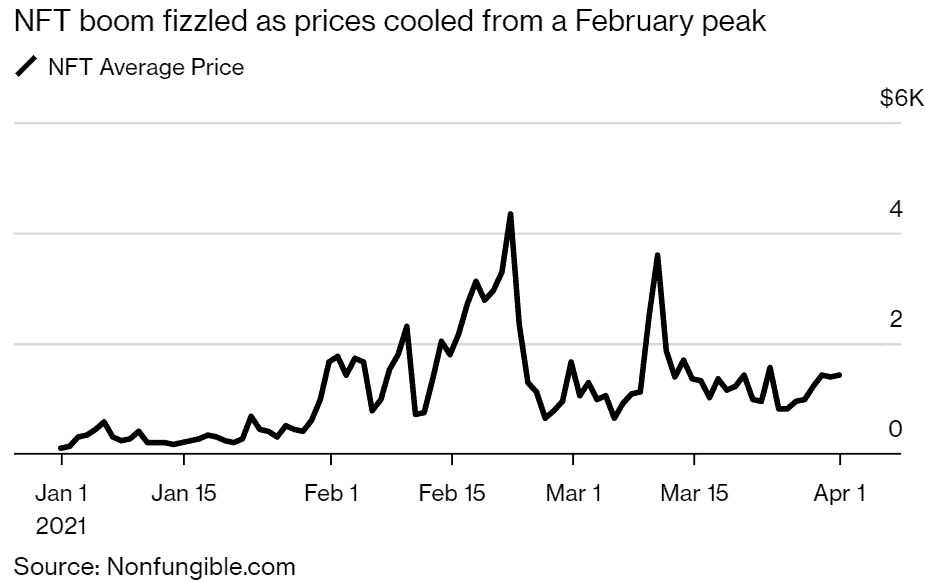
\includegraphics[scale=0.45]{gambar/img-nft-price-history.png}
  \caption{Pergerakan Harga NFT}
  \label{fig:Architecture}
\end{figure}

Grafik diatas merupakan salah satu contoh pergerakan harga rata-rata NFT dalam kurun waktu 4 bulan pada awal tahun 2021. Pada grafik tersebut terlihat bahwa pergerakan harga NFT cenderung fluktuatif, berbeda dengan aset layaknya di dunia nyata yang lebih stabil. Hal ini disebabkan oleh faktor potensi penggunaan dan keuntungan atas kepemilikan yang masih sangat minim yaitu hanya sebagai karya seni dan juga likuiditas yang rendah. 
Hal ini mengakibatkan pergerakan harganya tidak stabil dan hanya ditentukan oleh isu yang sedang tren di masyarakat.

Berangkat dari permasalahan tersebut penulis memiliki keinginan untuk mengembangkan suatu platform NFT marketplace yang memiliki fitur-fitur yang dapat memperluas potensi penggunaan \emph{NFT}, meningkatkan keuntungan atas kepemilikan NFT, dan meningkatkan likuiditas dari aset NFT sehingga dapat meningkatkan aspek ekonomi dari \emph{metaverse} layaknya di dunia nyata. 

\section{Rumusan Masalah}
Berdasarkan latar belakang yang telah dipaparkan dapat diketahui bahwa terdapat permasalahan pada penggunaan \emph{NFT} pada \emph{metaverse} disamping keuntungan yang diperoleh yaitu keterbatasan fitur \emph{NFT Marketaplce} sehingga mengakibatkan NFT yang digunakan sebagai aset dalam \emph{metaverse}
\begin{itemize}
  \item Kemampuan integrasi dengan platform lain yang terbatas
  \item Potensi penggunaan dan keuntungan atas kepemilikan \emph{NFT} yang tidak optimal
  \item Likuiditas yang rendah
  \item Harga yang tidak stabil
\end{itemize}

\section{Batasan Masalah atau Ruang Lingkup}

Adapun batasan masalah agar pembahasan topik ini dapat terarah dan mencapai tujuan. Batasan-batasan masalah tersebut adalah sebagai berikut:
\begin{enumerate}
  \item Pembuatan NFT marketplace berbasis \emph{blockchain} Ethereum.
  \item Target pengguna ialah seluruh pengguna yang terlibat dalam \emph{metaverse}.
  \item Pengujian transaksi dilakukan melalui jaringan \emph{Hardhat} sehingga penelitian berbentuk eksperimen, tidak menggunakan nominal real \emph{Ether}.
  \item Fitur yang akan dikembangkan pada NFT \emph{marketplace} ini adalah sistem sewa dan pembagian kepemilikan aset NFT.
\end{enumerate}

\section{Tujuan}

Berdasarkan permasalahan yang sudah dijelaskan, tujuan dari tugas akhir ini adalah untuk mengembangkan suatu platform \emph{NFT Marketplace} yang memiliki fitur sistem penyewaan NFT dan pembagian kepemilikan sehingga dapat meningkatan likuiditas aset dan aspek ekonomi dari suatu \emph{metaverse}.

\section{Manfaat}

\begin{enumerate}
  \item Bagi para pengguna \emph{metaverse} yaitu meningkatan potensi kemampuan pengguna untuk dapat menggunakan suatu aset bahkan memiliki suatu aset.
  \item Bagi para pengguna \emph{metaverse} yang memiliki aset NFT dapat meningkatan potensi keuntungan yang diperoleh dari aset yang dimiliki.
  \item Meningkatkan aspek ekonomi pada \emph{metaverse}.
\end{enumerate}

\cleardoublepage

% Bab 2 tinjauan pustaka
\chapter{TINJAUAN PUSTAKA}

% Ubah konten-konten berikut sesuai dengan isi dari tinjauan pustaka
\section{Hasil penelitian/perancangan terdahulu}

\subsection{\emph{Ether Wallet} Menggunakan Ethereum Berbasis \emph{Multi Signature} }

Penulis pada \parencite{IdaBagus} menggunakan \emph{multisignature wallet} dengan harapan untuk menghindari kasus penipuan perseorangan yang memiliki wallet digital khususnya dengan teknik \emph{social engineering} seperti \emph{phising}, kemudian dapat bermanfaat dalam meningkatkan keamanan serta kepercayaan untuk lingkup kerjasama seperti diperusahaan karena untuk mengakses dompet membutuhkan konfirmasi dari kedua belah pihak. \emph{Multi Signature Wallet} sendiri merupakan dompet yang dapat dijalankan ketika telah mendapatkan persetujuan dari alamat dompet lainnya yang dimiliki oleh pengguna. 

% Contoh input gambar dengan format *.jpg
\begin{figure} [ht] \centering
  % Nama dari file gambar yang diinputkan
  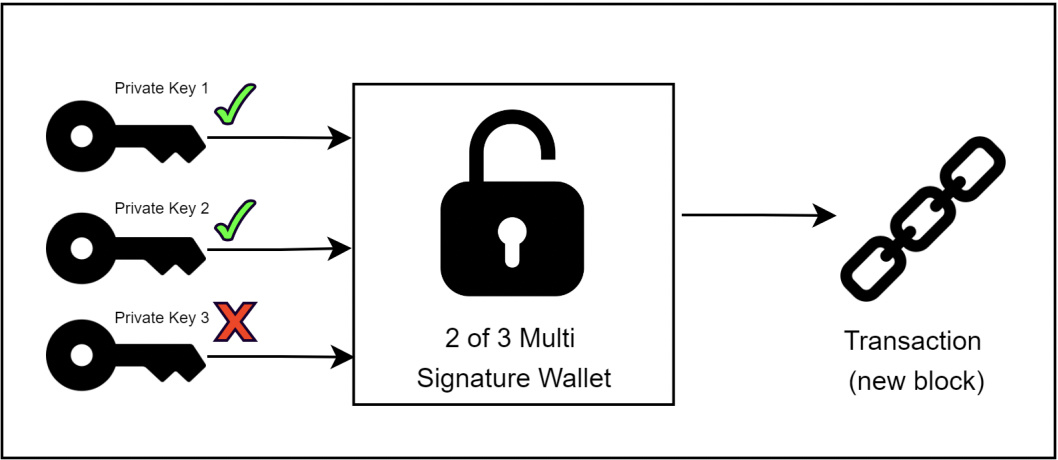
\includegraphics[scale=0.6]{gambar/img-multisignature-wallet.png}
  % Keterangan gambar yang diinputkan
  \caption{Multi Sig Wallet Konfirmasi 2 Akun}
  % Label referensi dari gambar yang diinputkan
  \label{fig:Multisignature Wallet}
\end{figure}

Walaupun begitu, dalam kasus penggunaan \emph{shared ownership}, \emph{multisignature wallet} memiliki berbagai kekurangan dalam praktiknya. Jika dibandingkan dengan pembagian kepemilikan dalam kasus suatu pembelian saham perusahaan, pembeli saham tidak perlu berhubungan langsung dengan pemilik-pemilik lainnya. Akan tetapi penggunaan \emph{multisignature wallet} ini seorang pembeli saham tersebut harus berkomunikasi dengan pemilik lain untuk menambahkan \emph{private key} yang tentunya hal ini lah yang cukup menyulitkan bagi calon pembeli saham baru tersebut. 

\section{Teori/Konsep Dasar}

\subsection{Blockchain}

% Contoh input gambar dengan format *.jpg
\begin{figure} [ht] \centering
  % Nama dari file gambar yang diinputkan
  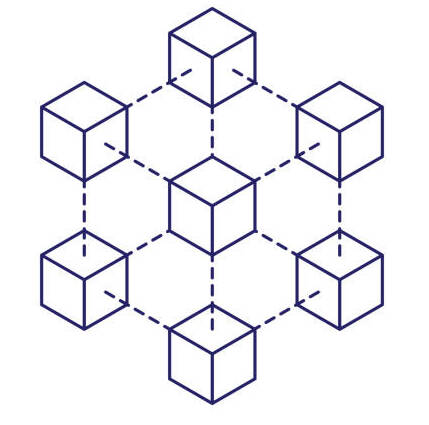
\includegraphics[scale=1.2]{gambar/img-blockchain-illustration.jpg}
  % Keterangan gambar yang diinputkan
  \caption{Ilustrasi \emph{Blockchain}}
  % Label referensi dari gambar yang diinputkan
  \label{fig:Metaverse}
\end{figure}

% Contoh penggunaan referensi dari pustaka
\emph{Blockchain} adalah \emph{ledger} atau buku besar terdistribusi yang dibagikan diantara node-node dalam jaringan komputer \parencite{LouiseAxon}. Ledger atau buku besar ini didistribusikan antar \emph{node}-\emph{node} dalam \emph{Blockchain} secara \emph{peer-to-peer} dengan teknik kriptografi. Data-data yang berada di dalam \emph{Blockchain} tidak dapat diubah hanya dapat ditambahkan. 

\emph{Blockchain} juga merupakan suatu \emph{Database}. Walaupun begitu, \emph{Blockchain} memiliki perbedaan yaitu data-data pada \emph{Blockchain} tidak disimpan oleh pihak tinggal melainkan didistribusikan antar \emph{node}-\emph{node}. Selain itu perbedaan \emph{Blockchain} dengan \emph{Database} umumnya adalah bagaimana data di dalam \emph{Blockchain} dibentuk. Sebuah \emph{Blockchain} menyimpan berbagai informasi bersama dalam suatu kelompok yang dinamakan \emph{Block}. \emph{Block} memiliki penyimpanannya sendiri, dimana ketika kapasitas penyimpanannya terpenuhi maka \emph{Block} tersebut akan tertutup dan dihubungkan dengan blok sebelumnya.
Hal tersebut berbeda dengan \emph{Database} yang umumnya menyimpan data-data dalam suatu table. Setiap \emph{Block} properti khusus selain data yang disimpan seperti contohnya adalah \emph{timestamp} yang menandakan kapan \emph{Block} tersebut dibuat.

Data di dalam \emph{Blockchain} bersifat \emph{immutable} yang berarti bahwa sekali data ditambahkan kedalam \emph{Blockchain}, hampir tidak mungkin
untuk mengubah data itu dan data sebelumnya pun praktis tidak berubah. Dengan kata
lain, blok yang ditambahkan ke Blockchain tidak dapat diubah, yang memungkinkan Blockchain menjadi buku besar transaksi yang tidak dapat dirusak maupun diubah. Namun,
hal itu dapat saja berbeda, bahwa Blockhain dapat diubah dalam skenario langka di mana
kerjasama mengubah jaringan Blockchain oleh peretas berhasil mendapatkan lebih dari
51 persen kekuatan jaringan dalam waktu yang relatif singkat. Hal ini lah yang menjadikan \emph{Blockchain} lebih aman dari model penyimpanan data pada umumnya. 

Di dalam \emph{Blockchain} tidak ada pihak sentral yang memiliki otoritas lebih tinggi dari yang lain sehingga jika terjadi perubahan bagaimana \emph{Blockchain} bekerja ditentukan oleh kesepakatan \emph{node}-\emph{node} di dalam \emph{Blockchain} tersebut. Kesepakatan ini juga sering dikenal dengan istilah konsensus dan tiap \emph{Blockchain} memiliki konsensusnya masing-masing.
Konsensu menjadi hal yang paling penting untuk mengubah sistem dari suatu \emph{Blockchain}, sehingga
Blockchain ini juga digambarkan seperangkat aturan konsensus, yang mengatur transaksi
mulai dari transaksi apa yang dilakukan hingga apa yang membuat transaksi tersebut
kemudian dapat divalidasi, inilah yang membuatnya menjadi terdesentralisasi. \emph{Blockchain}
dapat dikatakan sebuah mesin yang memproses aturan sesuai dengan konsensus tersusun
dari rantai blok yang diamankan secara kriptografis. Konsensus pada \emph{Blockchain} ini bersifat memaksa terhadap penambang untuk mengikuti dan bekerjasama dalam penegakan
aturannya. \parencite{antonopoulos2018mastering}

Secara ringkas \emph{Blockchain} memiliki berbagai keunggulan diantaranya adalah sebagai berikut
\begin{itemize}
    \item \emph{Transparant}, dalam \emph{blockchain} menerapkan sistem yang transparan sehingga dapat dilihat oleh berbagai orang.
    \item \emph{Immutability}, data yang dibuat didalam \emph{blockchain} tidak dapat ubah setelah dibuat.
    \item \emph{Secure}, dengan adanya implementasi kriptografi seperti validasi dengan fungsi hash membuat data yang ada pada Blockchain lebih aman.
    \item \emph{Traceability}, pada setiap blok dalam \emph{blockchain} menyimpan hash dari blok sebelumnya sehingga data pada Blockchain dapat dilacak dengan mudah.
    \item \emph{Anonymous}, setiap transaksi yang dibuat dapat dilihat oleh orang lain akan tetapi identitasnya tidak dapat diketahui dikarenakan yang ditampilkan adalah alamat \emph{wallet} atau yang merupakan \emph{public key}.
  \end{itemize}

\subsection{\emph{Node}}

\emph{Node} di dalam \emph{Blockchain} memiliki tanggung jawab untuk bertindak sebagai titik komunikasi yang dapat membuat, menerima, mengirim, dan mengyimpan data di dalam jaringan \emph{Blockchain}. Node pada dasarnya merupakan komputer yang berisi salinan dari riwayat transaksi dan data \emph{Blockchain}. \emph{Node} memiliki jenis dan fungsinya masing-masing. \parentext{DouglasTjokrostetio}

\subsubsection{\emph{Node} Penuh (\emph{Full Node})}

\emph{Node} penuh merupakan \emph{Node} yang berperan vital dalam \emph{Blockchain} dikarenakn bertindak sebagai \emph{fully validating node} atau \emph{Node} yang sepenuhnya melakukan validasi setiap transaksi yang dilakukan. \emph{Node} penuh pada awalnya akan mengunduh seluruh salinan \emph{Blockchain}. Untuk \emph{Bitcoin} sendiri pada tahun 2021 suatu \emph{Full Node} membutuhkan ruang penyimpanan 350 \emph{gigabyte} (GB) untuk mengunduh seluruh data \emph{Blockchain}.

\subsubsection{\emph{Node} Listening (\emph{Supernode})} dan Node Tersembunyi (Non-Listening Node)

\emph{Node Listeng} atau \emph{supernode} adalah \emph{Full Node} yang terlihat oleh publik. Ketika suatu \emph{Node} melakukan komunikasi dengan \emph{Node} listening, node ini akan mengomunikasikan dengan memberikan informasi ke \emph{Node} tersebut. Berbeda dengan \emph{Node listening} , \emph{Node non-listening} tidak terlihat oleh publik. \emph{Node} ini beroperasi di belakng \emph{firewall} atau dikonfigurasi supaya tidak mendengarkan komunikasi dari luar.

\subsubsection{\emph{Node Miner}}

Ekosistem \emph{Blockchain} yang menggunakan konsensus tertentu seperti \emph{proof-of-work} yang diterapkan oleh \emph{Bitcoin} membutuhkan \emph{Full Node} yang berperan sebagai \emph{Miner}. \emph{Node} ini berperan dalam menambahkan data transaksi ke \emph{Blockhain} dan akan menerima \emph{reward} seperti kripto.

\subsubsection{\emph{Lightweight Node}}

\emph{Node} ringan yang juga dikenal sebagai klien \emph{SPV} (\emph{Simplified Payment Verification}), adalah node yang menggunakan jaringan \emph{Blockchain} tapi tidak sepenuhnya bertindak layaknya \emph{Full Node}. Klien SPV tidak berkontribusi dalam keamanan suatu \emph{Blockchain} dikarenakan tidak menyimpan salinan \emph{Blockchain} dan melakukan proses validasi transaksi. Klien SPV hanya melakukan pemeriksaan apakah suatu informasi dapat ditermukan dalam jaringan \emph{Blockchain}.

\subsection{\emph{Block}}

% Contoh input gambar dengan format *.jpg
\begin{figure} [ht] \centering
  % Nama dari file gambar yang diinputkan
  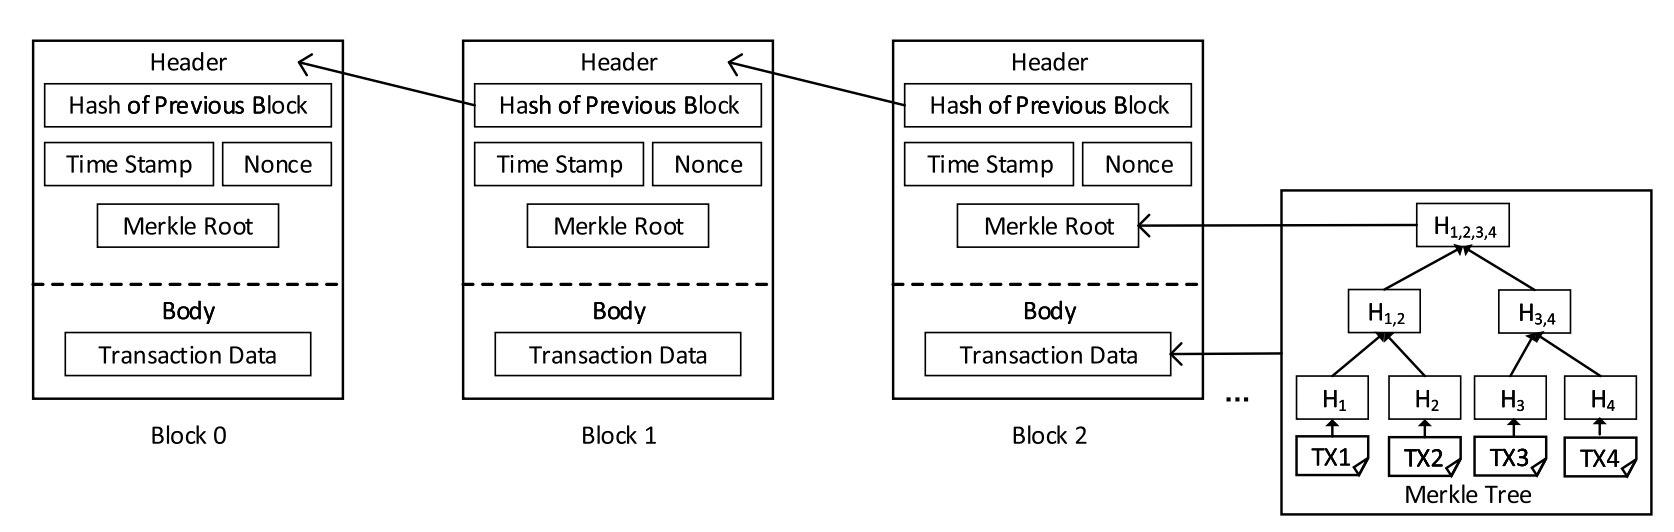
\includegraphics[scale=0.55]{gambar/img-block-structure.png}
  % Keterangan gambar yang diinputkan
  \caption{Struktur \emph{Block} pada \emph{Blockchain}}
  % Label referensi dari gambar yang diinputkan
  \label{fig:Metaverse}
\end{figure}

Di dalam jaringan \emph{Blockchain} suatu transaksi yang telah divalidasi oleh \emph{Node} akan disimpan ke dalam \emph{Block}. \emph{Block} sendiri tersusun dari \emph{Header} dan \emph{Body}. \emph{Header Block} tersusun dari \emph{Hash} dari \emph{Block} sebelumnya, \emph{timestamp}, \emph{Nonce}, dan \emph{Merkle Tree}. Nilai dari \emph{hash} diperoleh dari \emph{Header Block} sebelumnya yang telah dilakukan \emph{Hashing}. Memasukan \emph{Header Block} sebelumnya ke \emph{Block} saat ini membuat \emph{Block}-\emph{Block} dalam \emph{Blockchain} sehingga menciptakan suatu ikatan (\emph{chain}) dan terntunya menjadikannya saling terhubung antar satu \emph{Block} dengan \emph{Block} lainnya. Hal ini pun yang membuat \emph{Blockchain} aman dikarenakan jika akan melakukan pengubahan pada satu \emph{Block} maka seluruh \emph{Block} juga perlu diubah jika tidak akan dapat divalidasi melalui nilai \emph{Hash}-nya. \emph{Timestamp} sendiri berisi informasi kapan waktu \emph{Block} tersebut dibuat. \emph{Nonce} (number only used once) adalah angka yang dipecahakn oleh \emph{miner}. Angka ini diubah oleh \emph{miner} untuk memperoleh \emph{Merkle tree root hash} yang berdada di bawah nilai target. \emph{Merkle tree root hash} sendiri merupakan suatu data yang meringkas seluruh transaksi dalam \emph{Block} tersebut dan digunakan untuk memudahkan proses validasi. \emph{Body} pada suatu \emph{Block} sendiri berisi daftar transaksi yang disimpan.     
\parencite{LiangYiangBlockchainDynamicSpectrum}

\subsection{\emph{Wallet}}

\emph{Wallet} yang digunakan dalam transaksi pada \emph{Blockchain} merupakan suatu perangkat lunak yang memungkinkan antar pengguna untuk bertransaksi satu dengan yang lainnya dan merekam saldo dari pengguna. Berbeda dengan uang fiat, \emph{cryptocurrency} dalam \emph{Blockchain} tidak disimpan secara fisik. Di dalam \emph{Wallet} terdapat \emph{public key} dan \emph{private key}. Kedua \emph{Key} ini merupakan pasangan yang diperoleh dari algoritma asimetris dalam kriptografi. \emph{Public key} digunakan sebagai identifikasi dalam melakukan penerimaan atau pengiriman layaknya nomor rekening bank. Sedangkan \emph{Private key} digunakan untuk melakukan proses \emph{Authorization} dalam mengakses \emph{Wallet} tersebut. Selain itu juga terdapat \emph{address} dalam \emph{wallet} yang berfungsi sebagai pengenal unik yang digunakan untuk memfasilitasi proses pembayaran. \emph{Address} sendiri lebih singkat dibandingkan \emph{Public key} dikarenakan diperoleh dari melakukan \emph{hash} terhadap \emph{Public key}. 
\parencite{JokicStevo}

Terdapat dua jenis utama \emph{Wallet} dalam \emph{Blockchain} yaitu \emph{hot wallet} dan \emph{cold storage}. \emph{Hot wallet} adalah \emph{wallet} kripto yang biasanya terkoneksi dengan internet. \emph{Hot wallet} tidak harus selalu terhubung dengan internet. Dengan melakukan pengunduhan data, pengguna dapat menyimpan informasi milik mereka di perangkat pribadi. Wallet jenis ini umumnya memiliki tingkat kerentanan yang tinggi. Di lain sisi \emph{Cold storage} adalah \emph{Wallet} yang tidak terhubung ke inernet.

\subsection{Ethereum}

Ethereum adalah salah contoh dari \emph{Blockchain} yang diciptakan setelah \emph{Bitcoin}. Namun \emph{Ethereum} lebih dari sekedar \emph{Bitcoin} yang mendistribusikan catatan, \emph{Ethereum} adalah jaringan mesin virtual terdistribusi sehingga selain memiliki kemampuan untuk menyimpan suatu catatan dan mendistribusikannya, \emph{Ethereum} juga memiliki kemampuan untuk mengeksekusi suatu program yang berada di dalamnya. Hal tersebut berkat adanya \emph{EVM (Ethereum Virtual Machine)} yang mampu mengeksekusi program yang berada dalam \emph{node-node} pada \emph{Blockchain} \emph{Ethereum} sehingga \emph{Blockchain} ini tidak hanya sebagai \emph{Blockchain} catatan berjalan tetapi juga sebagai mesin virtual berjalan. Program yang berjalan di atas \emph{EVM} dikenal juga sebagai \emph{Smart Contract} dimana suatu fungsi di dalam \emph{Smart Contract} akan dieksekusi ketika suatu kondisi tertentu terpenuhi. Dengan kemampuan mengeksekusi \emph{Smart Contract} \emph{Ethereum} menciptakan era baru pada perkembangan \emph{Blockchain} yang memungkinkan para pengembang dapat menjalankan aplikasi terdistribusi atau juga dikenal sebagai \emph{DApps}.  Jaringan komputer terdistribusi \emph{Ethereum} dengan mudah menyediakan keamanan, keandalan, dan daya komputasi yang
diperlukan untuk melaksanakan pengaturan yang dirancang. Blockchain Ethereum pun
juga dapat dicari secara publik (Jani, 2017)

Ethereum dikembangan pada tahun 2013 oleh Vitalik Buterin, seorang programmer yang memiliki minat pada perkembangan \emph{Blockchain} dan \emph{Bitcoin}.
Vitalik berpikir untuk memperluas kemampuan dari Bitcoin dan Mastercoin. Pada bulan Okteber di tahun tersebut, Vitalik mengusulkan pendekatan yang lebih umum kepada tim
Mastercoin, yang memungkinkan kontrak fleksibel dan dapat ditulis untuk menggantikan
bahasa kontrak khusus Mastercoin. Tim Mastercoin terkesan namun belum bisa menerima usulan dalam bentuk proposal tersebut karena masih terkesan ’kasaran’. Maka dari
itu, Vitalik yang juga salah satu pendiri Bitcoin Magazine, pada bulan Desember menerbitkan whitepaper yang mengusulkan implementasi Blockchain baru yang lebih fungsional.
Proposal baru ini kemudian dinamakan Blockhain Ethereum. Setelah mendapatkan minat
dan menarik teknis dan finansial dukungan, Yayasan Ethereum, sebuah organisasi nirlaba
Swiss, didirikan dan menjadi pengembang Ethereum. Proses pengembangan ini berlangsung sejak saat itu, hingga pada tanggal 30 Juli 2015, Ethereum blok pertama berhasil
di tambang (Antonopoulos Wood, 2018). Ethereum ini kemudian dinamakan Frontier.
serta saat bersamaan Wallet Ethereum versi beta juga dibentuk. Pengembangan sampai saat ini sudah ada 2 kali pembaharuan project Ethereum, yaitu Homestead ditahun
2016, dan Byzantium di tahun 2018 (Infante, 2019). Kemudian perubahan versi keempat,
direncanakan di release tahun ini dengan nama Theta.

\subsection{\emph{EVM (Ethereum Virtual Machine)}}

% Contoh input gambar dengan format *.jpg
\begin{figure} [ht] \centering
  % Nama dari file gambar yang diinputkan
  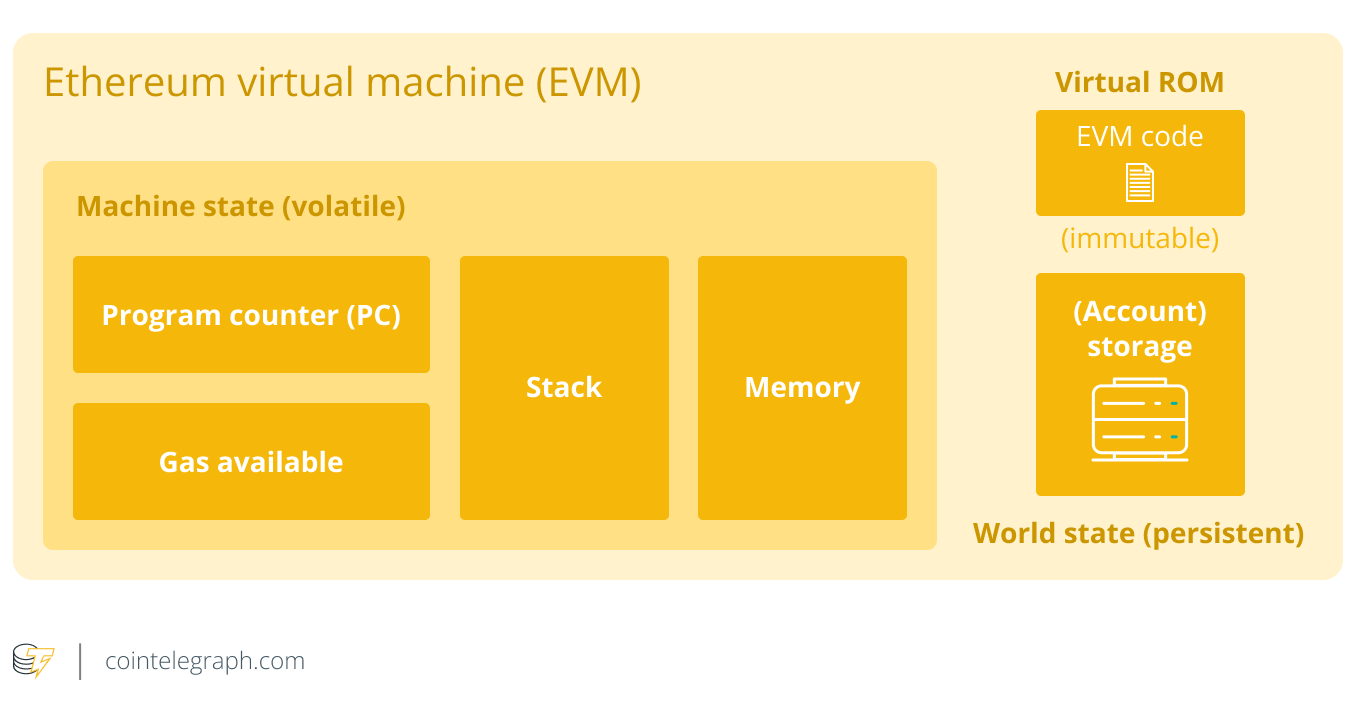
\includegraphics[scale=0.3]{gambar/img-evm.png}
  % Keterangan gambar yang diinputkan
  \caption{Ethereum Virtual Machine}
  % Label referensi dari gambar yang diinputkan
  \label{fig:Metaverse}
\end{figure}

\emph{EVM (Ethereum Virtual Machine)} adalah mesin komputasi virtual yang memiliki kemampuan untuk mengeksekusi suatu perintah atau fungsi pada \emph{Smart Contract}. \emph{EVM} terisolasi dari lingkungan di luarnya sehingga kode \emph{Smart Contract} yang berjalan di atasnya tidak memiliki kemampuan untuk mengakses jaringan, sistem berkas, atau proses lainnya. Ethereum sendiri memiliki dua jenis akun yaitu EOA (Externally-owned account) yang dikendalikan oleh siapapun yang memiliki \emph{private key} dan \emph{Contract account} yang dikendalikan oleh perintah-perintah yang berada di dalam \emph{Smart Contract}. Setiap \emph{Smart Contract} yang di \emph{deploy} pada jaringan \emph{Ethereum} memiliki alamat yang merupakan bagian dari \emph{Contract Account}. Kedua jenis akun hanya dapat berinteraksi dalam \emph{Smart Contract} yang dieksekusi oleh EVM.

\subsection{\emph{Ethereum Account}}

% Contoh input gambar dengan format *.jpg
\begin{figure} [ht] \centering
  % Nama dari file gambar yang diinputkan
  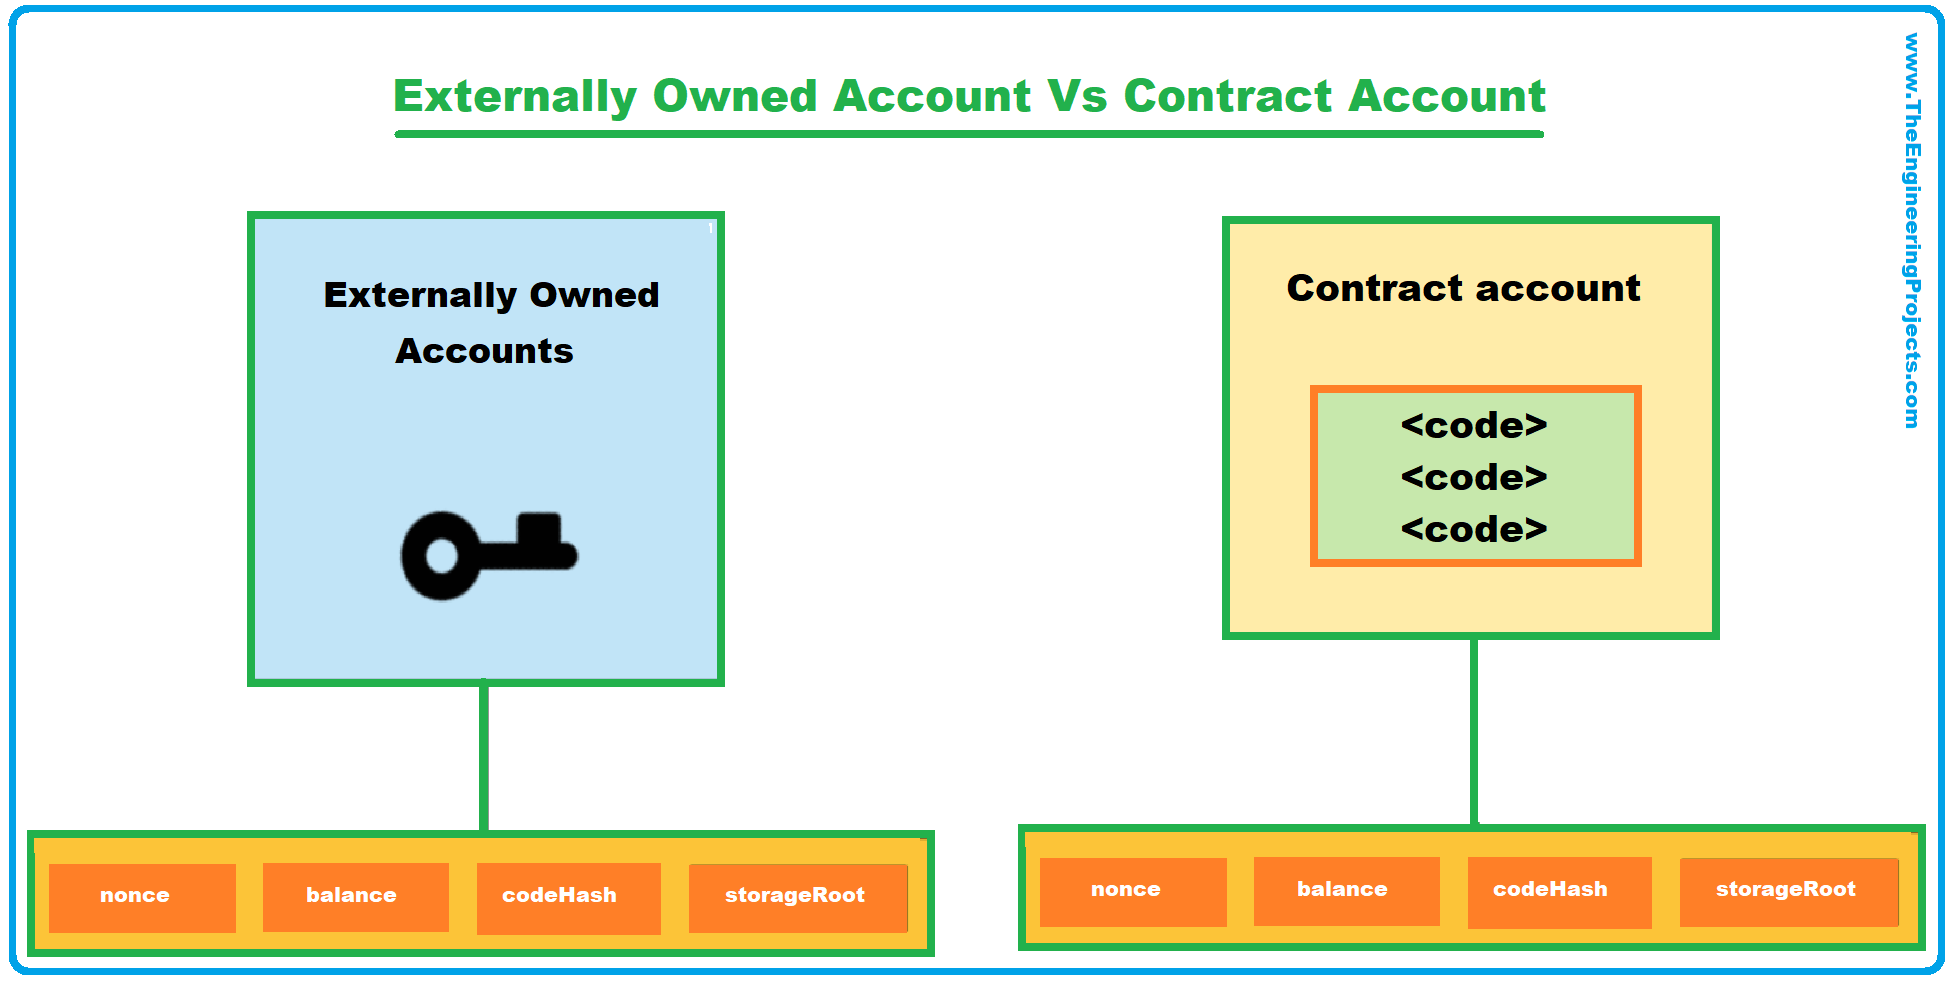
\includegraphics[scale=0.2]{gambar/img-ethereum-account.png}
  % Keterangan gambar yang diinputkan
  \caption{\emph{Account Ethereum}}
  % Label referensi dari gambar yang diinputkan
  \label{fig:Metaverse}
\end{figure}

Dalam melakukan transaksi dalam \emph{Blockchain Ethereum} pengguna memerlukan \emph{account}. \emph{Account} pada \emph{Blockchain Ethereum} sendiri terbagi menjadi dua jenis yaitu EOA (Externally Owned Account) dan \emph{Contract Account}. EOA adalah akun yang dikendalikan dan dimiliki masing-masing individu. Jenis akun ini dapat mengirim transaksi ke sesama \emph{EOA} ataupun akun kontrak. Akun ini memiliki \emph{Public key} dan \emph{Private key} yang terkait. Selain itu juga memiliki \emph{address} yang dihasilkan dari \emph{Public key} yang dimiliki. Ketika EOA dibuat, \emph{Private key} dienkripsi dengan kata sandi yang diberikan dalam pembuatan akun. Untuk mengakses dan melakukan transaksi pada EOA, \emph{Private key} dan kata sandi akan diperlukan. Akun kontrak sendiri dihasilkan dari proses \emph{deployment smart contract} oleh \emph{EOA} dan dikendalikan oleh kode-kode di dalamnya dalam melakukan transaksi. Kode-kode di dalam akun kontrak dieksekusi ketika dipanggil oleh EOA ataupun kontrak lain.  
\parencite{BahgaArshdeep}

\subsection{\emph{Transaction}}

% Contoh input gambar dengan format *.jpg
\begin{figure} [ht] \centering
  % Nama dari file gambar yang diinputkan
  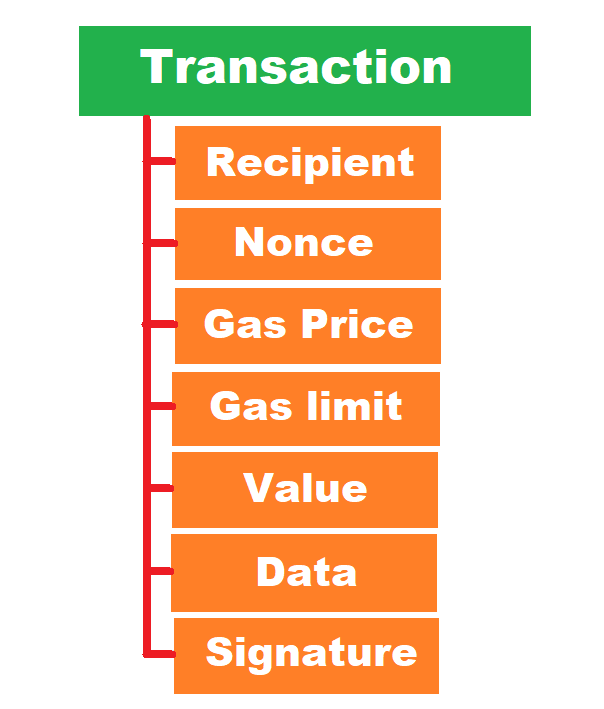
\includegraphics[scale=0.4]{gambar/img-transaction-structure.png}
  % Keterangan gambar yang diinputkan
  \caption{Struktur Transaksi}
  % Label referensi dari gambar yang diinputkan
  \label{fig:Metaverse}
\end{figure}

Transaksi adalah paket data yang telah ditandatangani untuk mengirim sejumlah \emph{ether} dari satu akun ke akun yang lain. Transaksi akan ditandatangi menggunakan \emph{ECDSA} (\emph{Elliptic Curve Digital Signature Alghoritm}) yang mana merupakan tanda tangan yang didasarkan pada \emph{ECC}. Sebuah transaksi berisi penerima pesan, tanda tangan pengirim dan tujuan pengiriman, jumlah \emph{Ether} yang akan dikirimkan, jumlah maksimum langkah komputasi yang dilakukan, dan biaya yang bersedia dibayarkan oleh pengirim. Jika transaksi berisi pemanggilan suatu \emph{function} dalam kontrak akan terdapat data parameter dari \emph{function} yang dipanggil.  
\parencite{PrustyBuilding}

\subsection{\emph{Gas}}

\emph{Gas} adalah satuan unit kerja yang digunakan dalam menilai seberapa mahal komputasi yang diperlukan. \emph{Gas} diperlukan sebagai bentuk \emph{reward} kepada \emph{miner} yang melakukan verfikasi transaksi. Biaya \emph{gas} memastikan bahwa \emph{miner} yang telah melakukan proses komputasi mendapat imbalan yang sesuai dengan upaya yang telah dilakukan. Biaya \emph{gas} dapat menjadi ditentukan berdasarkan kode dari \emph{Smart Contract} yang dieksekusi. Pada \emph{Blockchain Ethereum}, biaya \emph{gas} dapat diestimasi sebelum melakukan transaksi. Secara umum, biaya \emph{gas} dibagi menjadi tiga kategori yaitu cepat, sedang, dan lambat. Kategori cepat memakan waktu hingga 15 detik, kategori sedang hingga 30 detik, dan kategori lambat di atas 30 detik. Semakin cepat waktu yang diperlukan maka biaya gas akan semakin mahal.  
\parencite{DannenChris}

\subsection{Token}

Token, secara umum, adalah suatu unit nilai digital yang terdaftar dalam \emph{blockchain}  \parencite{PierluigiFreni}. Token dalam \emph{blockchain} memiliki berbagai bentuk berbagai kategori berdasarkan karakteristiknya. Secara garis token dalam Blockchain dibagi menjadi dua berdasarkan basisnya yaitu berbasis klaim dan berbasis objek. Token berbasis objek adalah token yang memiliki nilai intrinsik tersendiri dimana umumnya nilai tersebut ditentukan oleh permintaan dan penawaran. Contoh token berbasis klaim diantaranya adalah
\begin{itemize}
  \item Mata uang transaksional, adalah token yang umumnya digunakan sebagai alat pembayaran dan transaksi. Contoh dari token ini adalah Bitcoin (BTC) dan Litecoin (LTC).
  \item Koin privasi, token ini mampu melakukan transaksi dimana jumlah penukaran hanya akan diketahui oleh pengirim dan penerima.
  \item Mata uang \emph{Blockchain}, token ini dapat digunakan sebagai transaksi dan juga memungkinan pengguna untuk membuat aset digital dalam jaringan \emph{Blockchain} tersebut. Contoh token ini adalah Ether (ETH), Solana (SOL), dan Tron (TRX).
  \item Token utilitas, digunakan untuk menjalankan jaringan \emph{blockchain} dan membeli produk atau layanan dalam \emph{blockchain} tersebut. Contoh token ini adalah ERC-20
\end{itemize}
Sedangkan token berbasis klaim sendiri adalah token yang dirancang untuk mempertahankan nilainya. Dikaranekan hal tersebut lah token ini juga sering disebut sebagai \emph{stablecoin}. Nilai token ini dapat stabil dikarenakan nilainya dipatok dengan nilai aset yang liquid. Contoh dari token berbasis klaim adalah:
\begin{itemize}
  \item \emph{Stablecoin} yang diagunkan Fiat, \emph{stablecoin} ini memperoleh nilainya dari mata uang fiat seperti contoh nya dolar AS pada token Theter (USDT).
  \item \emph{Stablecoin} yang didukung asset, \emph{stablecoin} ini memperoleh nilainya dari suatu aset atau komoditas.
\end{itemize}
Dengan berbagai jenis token tersebut, dalam \emph{blockchain} Ethereum terdapat standar-standar yang diikuti supaya token tersebut dapat kompatibel dengan berbagai proyek aplikasi desentralisasi yang ada di dalam \emph{blockchain}. Contoh standar yang telah ditetapkan dalam pengembangan pada \emph{blockchain} Ethereum adalah sebagai berikut
\begin{itemize}
  \item ERC-20, \emph{interface} standar untuk \emph{fungible} token yaitu token yang nilainya setara sehingga dapat dipertukarkan dalam jumlah yang sama dikarenakan nilainya sama. \parencite{FabianVogelsteller}
  \item ERC-721, \emph{interface} standar untuk \emph{non-fungible} token yaitu token unik sehingga dalam jumlah yang sama nilai tokennya berbeda. \parencite{WilliamEntriken}
  \item ERC-1155 \emph{interface} standar untuk \emph{fungible} maupun \emph{non-fungible} token. \parencite{WitekRadomski}
  \item ERC-1633 \emph{interface} standar untuk pembagian kepemilikan NFT sehingga satu NFT dapat dimiliki lebih dari satu orang. \parencite{BillyRennekamp}
  \item ERC-4907 \emph{interface} standar yang menambahkan role baru pada NFT yaitu \emph{owner} yang merupakan pemilik NFT dan \emph{user} yang merupakan pihak yang mendapatkan akses tertentu pada NFT tersebut dengan waktu yang terbatas. \parencite{Anders}
\end{itemize}

\subsection{NFT}
NFT merupakan akronim dari \emph{Non-Fungible Token}. Sesuai namanya token ini bersifat \emph{non-fungible} atau unik sehingga satu NFT dengan yang lainnya berbeda dan tidak dapat ditukarkan. Hal ini berbeda dengan \emph{cryptocurrency} yang bersifat \emph{fungible} yang artinya token dengan jumlah yang sama dengan token dalam jumlah yang sama lainnya adalah sama sehingga dapat ditukarkan.

NFT adalah jenis token dalam \emph{blockchain} yang digunakan untuk merepresentasikan kepemilikan dari suatu asset yang unik \parencite{NavarroBlazquez}. NFT dapat melakukan tokenisasi berbagai hal seperti karya seni, barang koleksi, hingga real estate. Kepemilkan suatu aset diamankan dalam Blockchain sehingga tidak ada seorangpun yang dapat memanipulasi data kepemilkan dari suatu NFT.

\subsection{\emph{Smart Contract}}
\emph{Smart contract} adalah kontrak yang dieksekusi secara mandiri dengan ketentuan perjanjian yang ditulis ke dalam baris kode. Kode dan perjanjian yang terkandung di dalamnya ada di seluruh jaringan Blockchain. Kode tersebutlah berisi persyaratan yang harus dipenuhi supaya program dapat dieksekusi. Dengan adanya \emph{smart contract} perantara atau pihak ketiga saat menangani perjanian atau perselisihan tidak lagi diperlukan. \parencite{DouglasTjokrostetio}

Berikut merupakan karakteristik dari \emph{smart contract}:
\begin{itemize}
    \item \emph{Self executing}, program akan dieksekusi secara otomatis ketika syarat di dalam \emph{smart contract} terpenuhi.
    \item Tidak memerlukan hubungan berbasis kepercayaan, pihak-pihak dalam \emph{smart contract} dapat berinteraksi tanpa perlu saling mengenal dan percaya dikarenakan dieksekusi oleh sistem.
    \item Desentral, dikarenakan \emph{smart contract} berjalan diatas jaringan Blockchain kontrak akan diduplikasi dan dibagikan ke semua node dalam jaringan Blockchain.
    \item Dapat disesuaikan, kode dalam \emph{smart contract} dapat disesuaikan sesuai kebutuhan, hal ini lah yang menyebabkan berkembangnya aplikasi yang memanfaatkan \emph{smart contract} atau juga disebut Decentralized Applications (DApps). Contoh DApps pada ekosistem Blockchain antara lain adalah Decentralized Finance (DeFi), Game, hingga NFT Marketplace.
  \end{itemize}

% \subsubsection*{PEMBUATAN KODE SMART CONTRACT}

% Pembuatan kode \emph{smart contract} adalah proses membuat kode berdasarkan logic yang telah dibutuhkan dari perjanjian yang akan dibuat. Dalam pengembangan \emph{smart contract} umumnya bahasa pemrograman yang digunakan adalah Solidity. Pada bahasa pemrograman Solidity terdapat berbagai fungsi yang akan berguna dalam pengembangan \emph{smart contract} seperti \emph{function modifier}, \emph{function pure},\emph{logging event}, dan fungsi-fungsi lainnya.

% \subsection*{COMPILE SMART CONTRACT}

% Proses \emph{compile} kode dilakukan menggunakan bantuan Solidity \emph{Compiler}. Hasil dari proses \emph{compile} adalah ABI (\emph{Application Binary Interface}) dan \emph{byte code}. File ABI adalah file yang berisi mengenai fungsi-fungsi dan variabel yang ada dalam \emph{smart contract} dan ditulis dalam format \emph{Javascript Object Notation} (JSON). ABI berfungsi sebagai perantara dalam interaksi dengan jaringan \emph{blockchain}, baik dari luar \emph{blockchain} maupun dari satu \emph{smart contract} dengan \emph{smart contract} lainnya. Sedangkan \emph{byte code} adalah file yang berisi referensi fungsi yang kemudian akan dieksekusi oleh EVM (\emph{Ethereum Virtual Machine}). File \emph{bytecode} ini lah yang digunakan dalam proses \emph{}

% \subsection*{DEPLOY SMART CONTRACT}

% Proses \emph{deploy} adalah proses mengunggah \emph{smart contract} ke jaringan \emph{blockchain}. Setelah melakukan proses \emph{deployment} selesai akan menghasilkan \emph{address} dari \emph{smart contract} tersebut. \emph{Address} \emph{smart contract} digunakan sebagai tujuan dalam pengiriman data ketika suatu function dipanggil. 

\subsection{\emph{IPFS}}
\emph{IPFS} (\emph{InterPlanetary File System}) adalah sebuah protokol \emph{peer-to-peer} yang memungkinkan pengguna berbagi data dalam \emph{distributed file system}. Layaknya \emph{blockchain}, dalam IPFS juga terdapat \emph{node-node} yang terhubung untuk menyimpan suatu data. Sistem pada \emph{IPFS} menggunakan \emph{distributed hash table (DHT)} untuk memperoleh lokasi data. File yang diunggah di IPFS dibagi menjadi 5 bagian yang merupakan sebuah \emph{chunk} dan setiap \emph{chunk} memiliki \emph{link} yang menghubungkan ke \emph{chunk} yang lain. Di dalam IPFS juga terdapat \emph{versioning} sehingga pengguna dapat memperbarui file yang telah diupload dan merekan seluruh perubahan yang terjadi pada file tersebut. \parencite{MathisSteichen}

\subsection{\emph{Metaverse}}
\emph{Metaverse} secara sederhana didefinisikan sebagai realitas digital. Konsep ini menggambarkan ruang virtual yang menghubungkan dunia nyata dan dunia maya. Pengguna yang diwakili avatar atau suatu karakter dapat menjelajah dan berinteraksi dengan seluruh objek digital maupun pengguna lain dalam \emph{metaverse}. Pada awalnya game menjadi aktivitas yang terdekat yang dapat menawarkan pengalaman mirip \emph{metaverse}. Akan tetapi game saja tidaklah cukup dikatakan sebagai \emph{metaverse}, perlu adanya penggabungan dengan ekonomi, media sosial, identital digital dan lainnya untuk menciptakan pengalaman layaknya \emph{metaverse}. 

Layaknya di dunia nyata, dalam \emph{metaverse} seseorang juga dapat memiliki suatu aset dan memperjual belikan aset tersebut sehingga tercipta ekonomi baru dalam \emph{metaverse}. Untuk memungkinkan adanya hal tersebut namun juga mempertimbangkan aspek keamanan solusi yang banyak digunakan saat ini adalah Blockchain. Blockchain menjadi pilihan utama dalam pengembangan metaverse dikarenakan sebagai berikut:
\begin{itemize}
    \item Pembuktian kepemilikan sesorang terhadap aset tertentu dapat dengan mudah dilacak.
    \item Terkait dengan aspek ekonomi dalam metaverse, mata uang yang dapat diterima secara universal sangat diperlukan dimana hal ini dapat ditemukan pada \emph{cryptocurrency} dalam \emph{blockchain}.
    \item Aksesibilitas yang luas menggunakan \emph{wallet} \emph{blockhain} dilakukan dalam metaverse dikarenakan mudah untuk terhubung dalam berbagai platform di \emph{metaverse}.
    \item Aset dalam \emph{metaverse} yang memerlukan orisinalitas dapat diakomodasi dengan adanya NFT dalam \emph{blockchain}.
\end{itemize}\parencite{DouglasTjokrostetio}

% Contoh input gambar dengan format *.jpg
\begin{figure} [ht] \centering
  % Nama dari file gambar yang diinputkan
  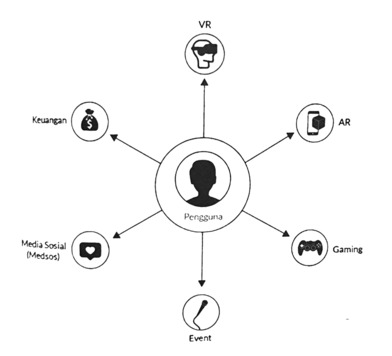
\includegraphics[scale=0.6]{gambar/img-metaverse-3.jpg}
  % Keterangan gambar yang diinputkan
  \caption{Metaverse tanpa \emph{blockchain}}
  % Label referensi dari gambar yang diinputkan
  \label{fig:Metaverse}
\end{figure}

% Contoh input gambar dengan format *.jpg
\begin{figure} [ht] \centering
  % Nama dari file gambar yang diinputkan
  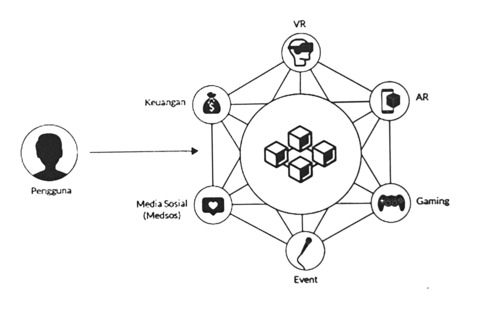
\includegraphics[scale=0.6]{gambar/img-metaverse-blockchain-4.jpg}
  % Keterangan gambar yang diinputkan
  \caption{Metaverse berbasis \emph{blockchain}}
  % Label referensi dari gambar yang diinputkan
  \label{fig:Metaverse Blockchain}
\end{figure}

\cleardoublepage

% Bab 3 desain dan implementasi
\chapter{METODOLOGI}

\section{DESKRIPSI SISTEM}

\subsection{Arsitektur Sistem}

\begin{figure} [ht] \centering
  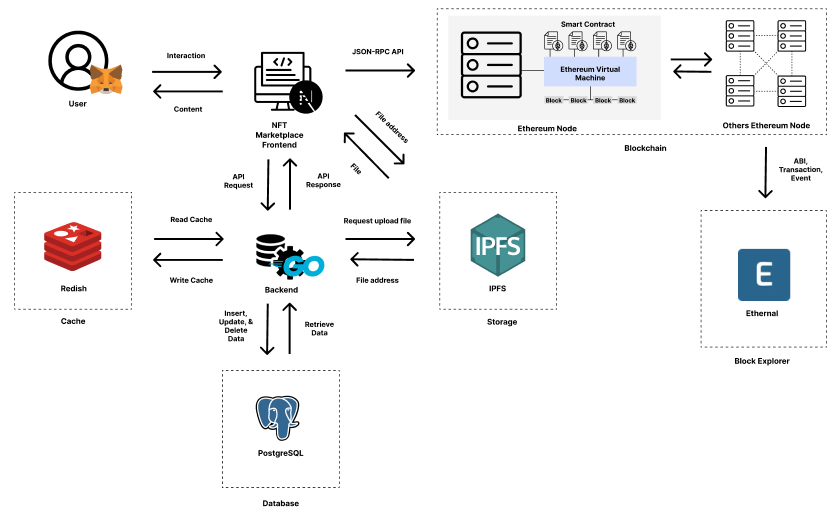
\includegraphics[scale=0.45]{gambar/img-architecture.png}
  \caption{Arsitektur NFT \emph{Marketplace}}
  \label{fig:Architecture}
\end{figure}

Dalam pengembangan suatu \emph{NFT Marketplace} ini diperlukan suatu arsitektur supaya sistem yang dikembangkan dapat bekerja sesuai dengan yang diharapkan. Pada \emph{NFT Marketplace} ini terdapat 2 \emph{role user} yaitu \emph{owner} yang merupakan pemilik dari suatu \emph{token} dan \emph{user} yang merupakan pihak yang memiliki akses terbatas terhadap suatu token dalam waktu yang telah ditentukan. Untuk dapat mengakses \emph{NFT Martketplace} baik \emph{owner} ataupun \emph{user} harus terhubung menggunakan \emph{wallet} dalam berinteraksi. 

Pengguna yang sudah terhubung dengan \emph{wallet} dapat berinteraksi dengan \emph{front end} aplikasi \emph{NFT Marketplace}. \emph{Frontend} akan terhungu dengan aplikasi \emph{backend} ketika pengguna melakukan \emph{Minting} dimana prosesnya pengguna mengunggah aset digital yang dimiliki dan diunggah ke \emph{IPFS} melakukan aplikasi \emph{backend} dan akan mengembalikan \emph{Content Identifier} (CID). \emph{CID} merupakan sebuah \emph{address} file dalam \emph{IPFS} yang digunakan untuk mengakses file tersebut. \emph{CID} yang diperoleh kemudian akan diunggah ke jaringan \emph{blockchain} dan menjadi suatu \emph{token}. Data-data mengenai \emph{NFT} yang tersedia dapat langsung diperoleh \emph{frontend} melalui \emph{smart contract} pada \emph{blockchain}. Selain itu dalam praktiknya aplikasi \emph{backend} juga akan menyediakan data-data seperti harga token melalui API yang disediakan oleh CoinMarketCap. Untuk memperoleh data mengenai estimasi \emph{gas fee} yang diperlukan aplikasi \emph{backend} juga terhubung dengan \emph{API ETH Gas Station}.

\subsection{\emph{Flow} Pembelian Token}

% Contoh input gambar dengan format *.jpg
\begin{figure} [H] \centering
  % Nama dari file gambar yang diinputkan
  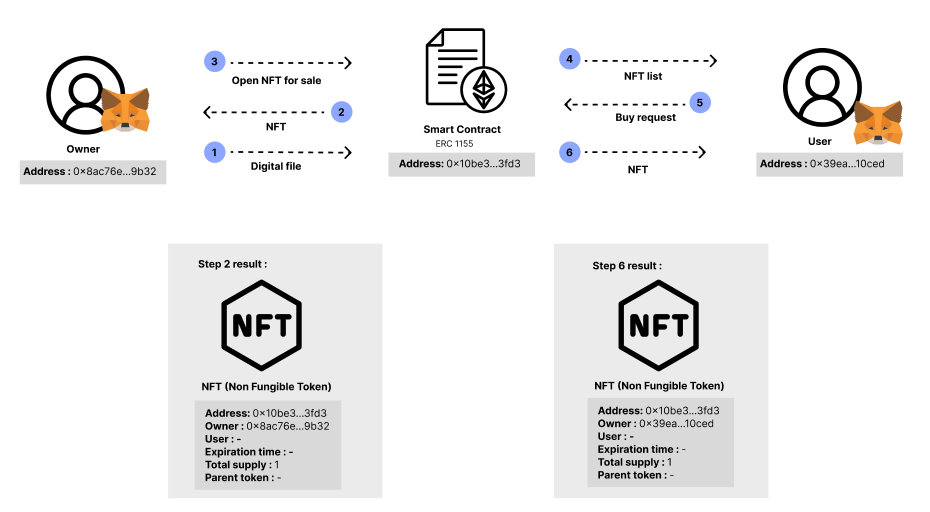
\includegraphics[scale=0.45]{gambar/img-nft-buy.png}
  % Keterangan gambar yang diinputkan
  \caption{\emph{Flow} pembelian \emph{Token}}
  % Label referensi dari gambar yang diinputkan
  \label{fig:Buy}
\end{figure}

Pembelian pada \emph{smart contract} yang akan dikembangkan menggunakan fungsi dari \emph{interface} \emph{ERC-1155}. \emph{Interface} ini memungkinkan \emph{token fungible} dan \emph{non-fungible} diperjual belikan dalam satu kontrak. Hal ini dimungkinkan dengan adanya penambahan properti \emph{supply} pada \emph{token}. Jika \emph{supply token} bernilai 1 maka \emph{token} tersebut akan diperlakukan sebagai \emph{NFT} sebaliknya maka token akan diperlakukan layaknya \emph{fungible token}.  

\subsection{\emph{Flow} Penyewaan NFT}

\begin{figure} [H] \centering
  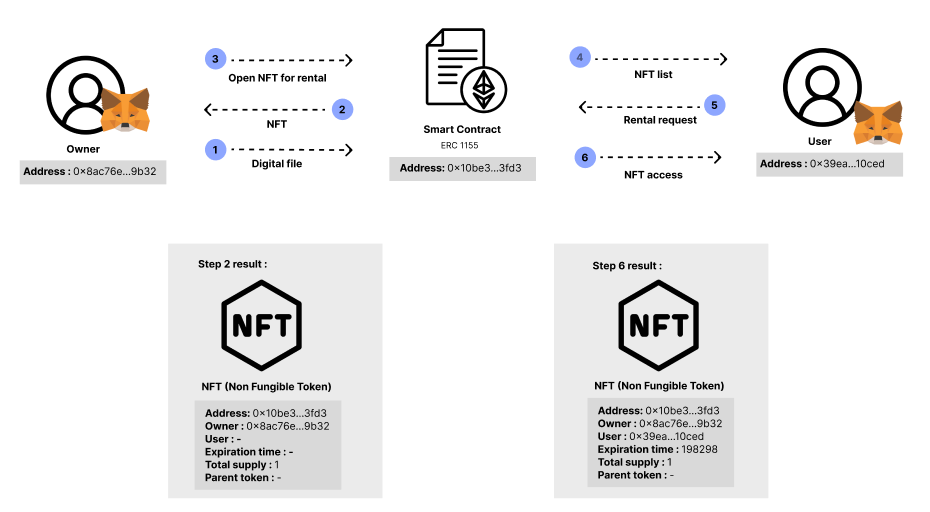
\includegraphics[scale=0.45]{gambar/img-nft-rental.png}
  \caption{\emph{Flow} penyewaan \emph{NFT}}
  \label{fig:Rental}
\end{figure}

Pemilik \emph{token} dapat menyewakan \emph{token} yang dimiliki kepada pengguna lain untuk memperoleh keuntungan selain melakukan penjual. Hal ini dimungkinan dengan adanya pemisahan \emph{role owner} dan \emph{user} pada \emph{token}. \emph{Owner} adalah pemilik token yang memiliki seluruh akses terhadap \emph{token} sedangkan \emph{user} adalah pihak yang memiliki akses terbatas terhadap token dan juga dibatasi dalam periode yang telah ditentukan.

\subsection{\emph{Flow} Pembagian Kepemilikan NFT}

% Contoh input gambar dengan format *.jpg
\begin{figure} [H] \centering
  % Nama dari file gambar yang diinputkan
  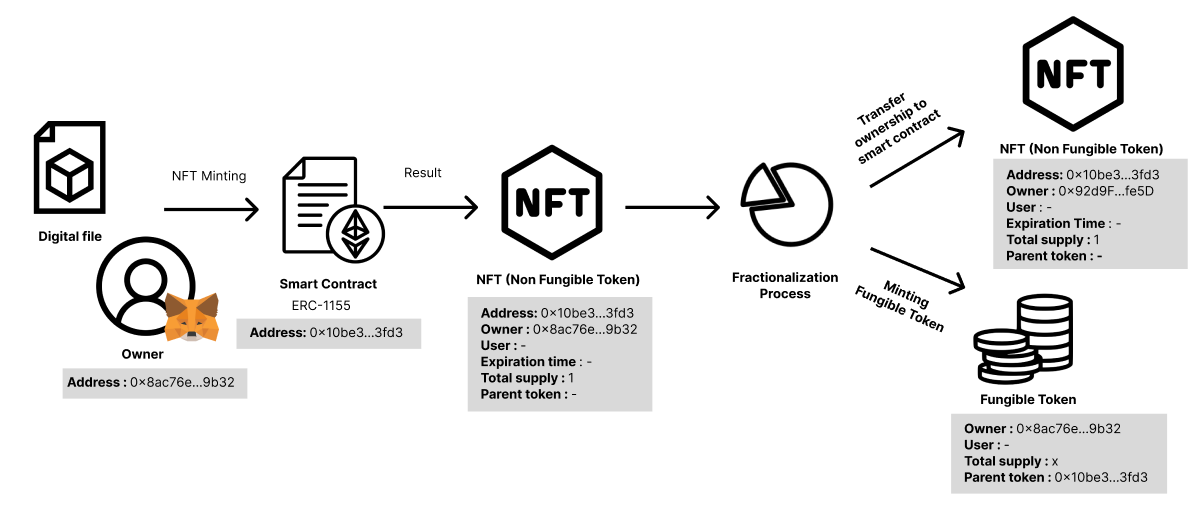
\includegraphics[scale=0.35]{gambar/img-fractional-nft.png}
  % Keterangan gambar yang diinputkan
  \caption{\emph{Flow} pembagian kepemilikan NFT}
  % Label referensi dari gambar yang diinputkan
  \label{fig:Fractional}
\end{figure}

Pembagian kepemilikan \emph{NFT} dilakukan melalui proses \emph{fractionalization}. Proses ini membuat \emph{NFT} ditransfer kepemilikannya ke pemilik \emph{smart contract}. Selain itu \emph{fungible token} dengan jumlah yang telah ditentukan akan di-\emph{minting}. \emph{Fungible token} ini lah yang akan merepresentasikan kepemilikan atasnya atas \emph{Parent Token}. Jika \emph{NFT} disewakan maka seluruh pemilik \emph{token fraction} akan memperoleh keuntungan sesuai dengan jumlah kepemilikannya atas \emph{token fraction}.

\subsection{\emph{Metadata}}

Berdasarkan \emph{interface} ERC-721 setiap NFT memiliki \emph{metadata}. \emph{Metadata} sendiri adalah data yang menyusun konten dari NFT tersebut dan biasanya dinyatakan dalam format JavaScript Object Notation (JSON). Data yang disimpan dalam \emph{metadata} biasanya meliputi nama, deskripsi, tautan ke gambar yang dapat disesuaikan dengan kebutuhan aplikasi desentral yang dibangun. Untuk menstandarisasi NFT maka \emph{metadata} yang ditetapkan pada \emph{project} NFT \emph{Marketplace} ini adalah sebagai berikut

\begin{figure} [H] \centering
  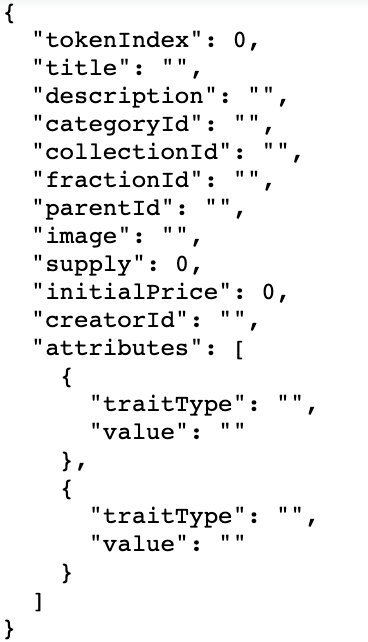
\includegraphics[height=7cm]{gambar/img-metadata.png}
  \caption{Metadata NFT}
  \label{fig:MetadataNFT}
\end{figure}

Atribut pada metadata di atas merupakan data-data yang terikat dengan \emph{NFT} yang dapat disesuaikan dengan kebutuhan masing-masing platform dimana data ini juga di simpan dalam format \emph{JSON (Javascript Object Notation)} berupa \emph{Array} dengan \emph{elemen object}. Setiap \emph{Object} tersebut memiliki dua \emph{field} yaitu \emph{traitType} yang merupakan nama data dan \emph{value} merupakan nilai dari data tersebut. Dengan adanya \emph{Attributes} membuat \emph{NFT} dapat \emph{compatible} dengan berbagai \emph{platform} lain.

\subsection{Integrasi Platform Lain}

Integrasi dengan platform lain menjadi hal yang penting dikarenakan \emph{NFT Marketplace} yang ingin dikembangkan diperuntukan supaya dapat digunakan oleh platform lain yang mengusung konsep \emph{metaverse}. Supaya \emph{platform} lain dapat terintegrasi dengan \emph{NFT Marketplace} yang dikembangkan terdapat \emph{API (Aplication Programming Interface)} yang disediakan. Langkah-langkah sebelum integrasi melalui \emph{API} adalah \emph{platform} tersebut perlu menyediakan fitur autentikasi melalui \emph{Wallet} atau menghubungkannya dan juga melakukan \emph{minting} melalui \emph{NFT Marketplace}. Berikut merupakan diagram tahapan dalam integrasi

\subsection{\emph{Minting}}

Hal pertama yang perlu dilakukan adalah platform lain melakukan proses \emph{minting} atau pembuatan \emph{NFT} baru. 
Pada saat melakukan \emph{minting} terdapat beberapa data yang diperlukan mengenai \emph{NFT} seperti nama, deskripsi, kategori, suplai, aset visual yang merepresentasikan \emph{NFT} dapat berupa 2D, 3D, dan video, harga awal, koleksi, hingga atribut. Setelah proses \emph{minting} selesai maka hasil akan diperoleh id token, id token ini lah yang harus disimpan ke dalam \emph{database} \emph{platform} lain untuk kemudian digunakan untuk mengakses data-data terkait \emph{NFT} tersebut seperti pemilik atau peminjam dari \emph{NFT} tersebut saat ini.

\begin{figure} [H]
  % Nama dari file gambar yang diinputkan
  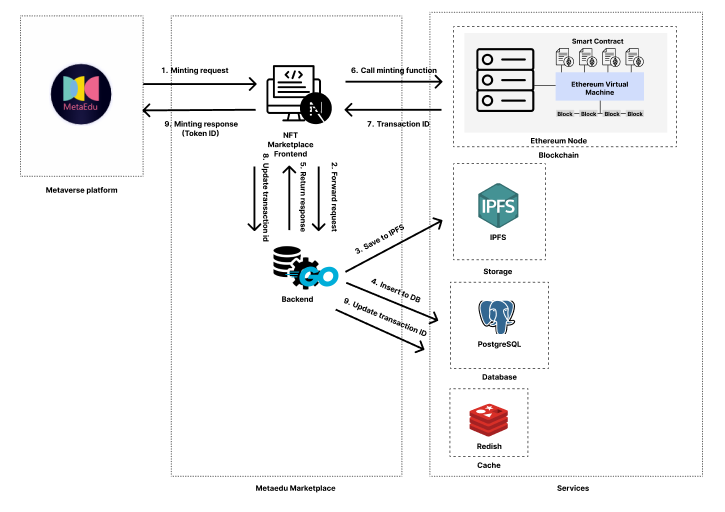
\includegraphics[width=\columnwidth,height=8cm]{gambar/img-integration-minting.png}
  % Keterangan gambar yang diinputkan
  \caption{\emph{Flow} pembagian kepemilikan NFT}
  % Label referensi dari gambar yang diinputkan
  \label{fig:Fractional}
\end{figure}

\subsection{\emph{Transaksi}}

\begin{figure} [H] \centering
  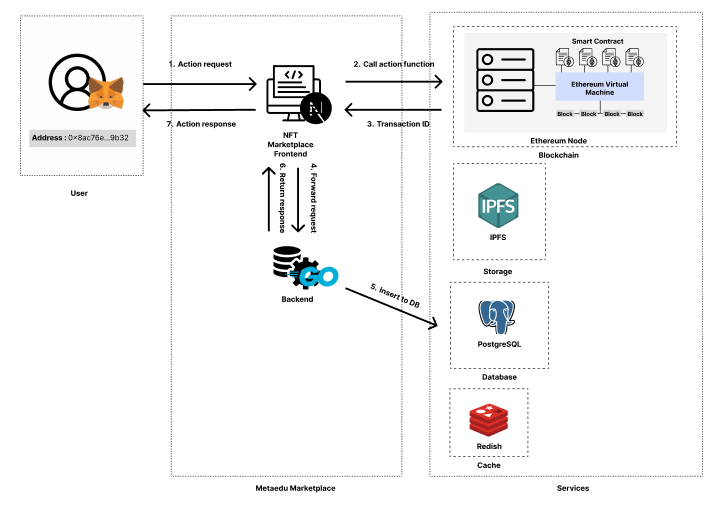
\includegraphics[scale=0.6]{gambar/img-integration-action.png}
  \caption{\emph{Flow} transaksi}
  \label{fig:ActionIntegration}
\end{figure}

Setelah melakukan proses \emph{minting} maka pengguna dapat melakukan transaksi berupa pembelian, peminjaman, ataupun pembagian kepemilikan terhadap \emph{NFT} baik antar pengguna maupun pengguna dengan \emph{platform} yang melakukan \emph{minting}.

\subsubsection{\emph{Fetching}}

\begin{figure} [H] \centering
  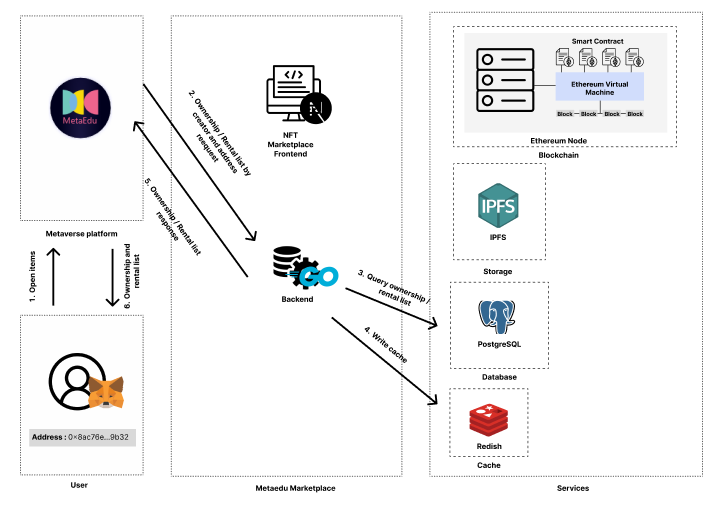
\includegraphics[scale=0.6]{gambar/img-integration-fetching.png}
  \caption{\emph{Flow fetching data}}
  \label{fig:FetchingIntegration}
\end{figure}

Tahap terakhir adalah proses \emph{fetching data}. Proses ini bertujuan supaya data \emph{NFT} yang di perjual belikan, disewakan, atau bahkan dibagikan kepemilikan dapat sinkron dengan \emph{platform metaverse}. Untuk melakukan hal tersebut pengguna platform yang terhubung dengan \emph{Wallet} memiliki \emph{Address}. Data berupa Address pengguna, ID creator token atau merupakan ID platform, dan ID token akan digunakan untuk mengakses \emph{endpoint} dari \emph{API} yang disediakan.

\begin{itemize}
  \item \emph{Endpoint} \emph{token} digunakan untuk memperoleh data \emph{NFT} yang di-\emph{minting} oleh \emph{platform} tersebut dengan menyertakan parameter \emph{id creator}.
   \item \emph{Endpoint} \emph{ownership} digunakan untuk memperoleh data kepemilikan atas suatu token dengan menyertakan parameter \emph{id token} atau data kepemilikan dari pengguna tertentu dengan menyertakan parameter \emph{Address} pengguna dan \emph{id creator}.
  \item \emph{Endpoint} \emph{rental} digunakan untuk memperoleh data peminjaman suatu \emph{token} dengan menyertakan parameter \emph{id token} atau data peminjaman pengguna dengan menyertakan parameter \emph{Address} pengguna dan \emph{id creator}.
  \item \emph{Endpoint} \emph{fraction} digunakan untuk memperoleh data mengenai pembagian kepemilikan suatu \emph{token} dengan menyertakan \emph{fraction token id} atau \emph{parent token id}
\end{itemize}

\section{Tools yang digunakan}

Dalam pengembangan \emph{NFT Marketplace} ini sesuai dengan arsitektu dan \emph{flow} yang dijelaskan sebelumnya diperlukan beberapa \emph{Software} dan \emph{Tools} dalam pengerjaannya. Dari sisi pengembangan \emph{Blockchain}-nya sendiri \emph{Software} yang digunakan adalah \emph{Solidity}, \emph{Hardhat}, \emph{Ehernal}, dan Metamask. Selain \emph{Blockchain} sendiri dibagi menjadi dua yaitu \emph{Frontend} dan \emph{Backend}. Pada sisi \emph{Frontend} yang menjadi tampilan muka dan tempat user berinteraksi adalah \emph{NextJS}, \emph{Typescript}, dan \emph{AntDesign}. Sedangkan pada sisi \emph{Backend} adalah \emph{Golang}, \emph{PostgreSQL}, \emph{Docker}, dan \emph{Redish}.

\begin{longtable}{|c|c|c|}
  \caption{\emph{Software} dan \emph{Tools} yang digunakan}
  \label{tb:EnergiKecepatan}                                   \\
  \hline
  \rowcolor[HTML]{C0C0C0}
  \textbf{\emph{Software/Tools}} & \textbf{Fungsi} \\
  \hline
  Solidity            & Bahasa pemrograman untuk mengembangkan \emph{smart contract}                                        \\
  Hardhat             & Simulasi \emph{blockchain} pada \emph{environment} lokal                                            \\
  Ethernal            & Melacak informasi pada \emph{blockchain}                                                            \\
  Metamask            & Sebagai \emph{Wallet} yang digunakan dalam bertransaksi                                             \\
  Golang              & Bahasa pemrograman untuk mengembangkan \emph{backend}                                               \\
  Redish              & Menyimpan \emph{cache}                                                                              \\
  PostgreSQL          & Menyimpan data-data                                                                                 \\
  Docker              & Memudahkan dalam melakukan proses \emph{setup} dan \emph{deployment}                                \\
  NextJS              & \emph{Framework} yang digunakan untuk mengembangkan \emph{frontend}                                 \\
  Typescript          & Bahasa pemrograman yang digunakan pada sisi \emph{frontend}                                         \\
  AntDesign           & \emph{Library} yang menyediakan berbagai komponen yang diperlukan pada \emph{frontend}              \\
  \hline
\end{longtable}

\subsection{\emph{Solidity}}

\emph{Solidity} merupakan bahasa pemrograman yang digunakan untuk mengembangkan \emph{smart contract} pada \emph{blockchain} \emph{Ethereum}. \emph{Solidity} termasuk ke dalam kategori \emph{multi bracket language}, artinya dibangun dengan beberapa bahasa pemrograman lain seperti C++, \emph{Python}, dan \emph{Javascript}, dan ditujukan supaya dapat berjalan pada \emph{EVM}. \emph{Smart contract} yang dibangun menggunakan \emph{Solidity} akan melakukan penyimpanan data dan pengiriman \emph{Ether} dari \emph{EOA} ke \emph{smart contract} maupun dari \emph{smart contract} ke EOA. 

\subsection{\emph{Hardhat}}

\emph{Hardhat} adalah lingkungan pengembangan \emph{Blockchain Ethereum}. \emph{Hardhat} mampu membuat dan mensimulasikan jaringan \emph{Ethereum} sehingga pengembang dapat mengembangkan \emph{Smart Contract} pada \emph{environment} lokalnya measing-masing. \emph{Software} ini juga akan membantu pengembang dalam \emph{compiling}, \emph{debugging}, \emph{deploying}, dan \emph{testing} pada \emph{Blockchain Ethereum}.
\begin{figure}[!h]
\centering 
  % Nama dari file gambar yang diinputkan
  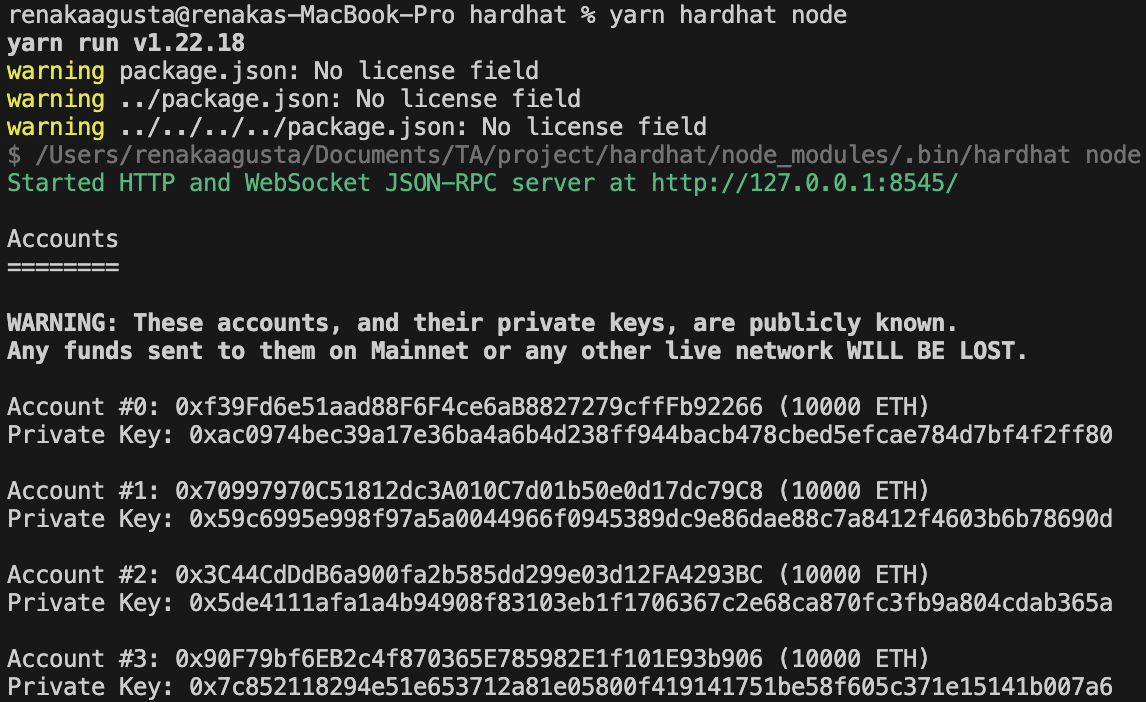
\includegraphics[scale=0.6]{gambar/img-hardhat.png}
  % Keterangan gambar yang diinputkan
  \caption{\emph{Hardhat}}
  % Label referensi dari gambar yang diinputkan
  \label{fig:Hardhat}
\end{figure}

\subsection{\emph{Ethernal}}

\emph{Ethernal} adalah \emph{Software Open Source} yang digunakan sebagai \emph{Blockchain Explorer} pada \emph{Blockchain Ethereum}. \emph{Block Explorer} membantu pengguna atau siapapun yang ingin mencari atau melacak informasi pada \emph{Blockchain} seperti transaksi, \emph{event}, akun, \emph{address}, dan sebagainya. Selain itu \emph{Ethernal} juga mendukung tampilan antarmuka dalam melakukan interaksi dengan \emph{Smart Contract} secara mudah. \emph{Software} ini juga tersedia sebagai \emph{plugin} dari \emph{hardhat} sehingga bagi pengembang yang telah menggunakan \emph{Hardhat} hanya perlu menambahkan \emph{plugin Ethernal} dan melakukan beberapa konfigurasi. Jika konfigurasi telah dilakukan, ketika proses \emph{compiling} dan \emph{deployment} \emph{ABI} akan diunggah ke \emph{Ethernal}.

\begin{figure}[H] 
  \centering
    % Nama dari file gambar yang diinputkan
    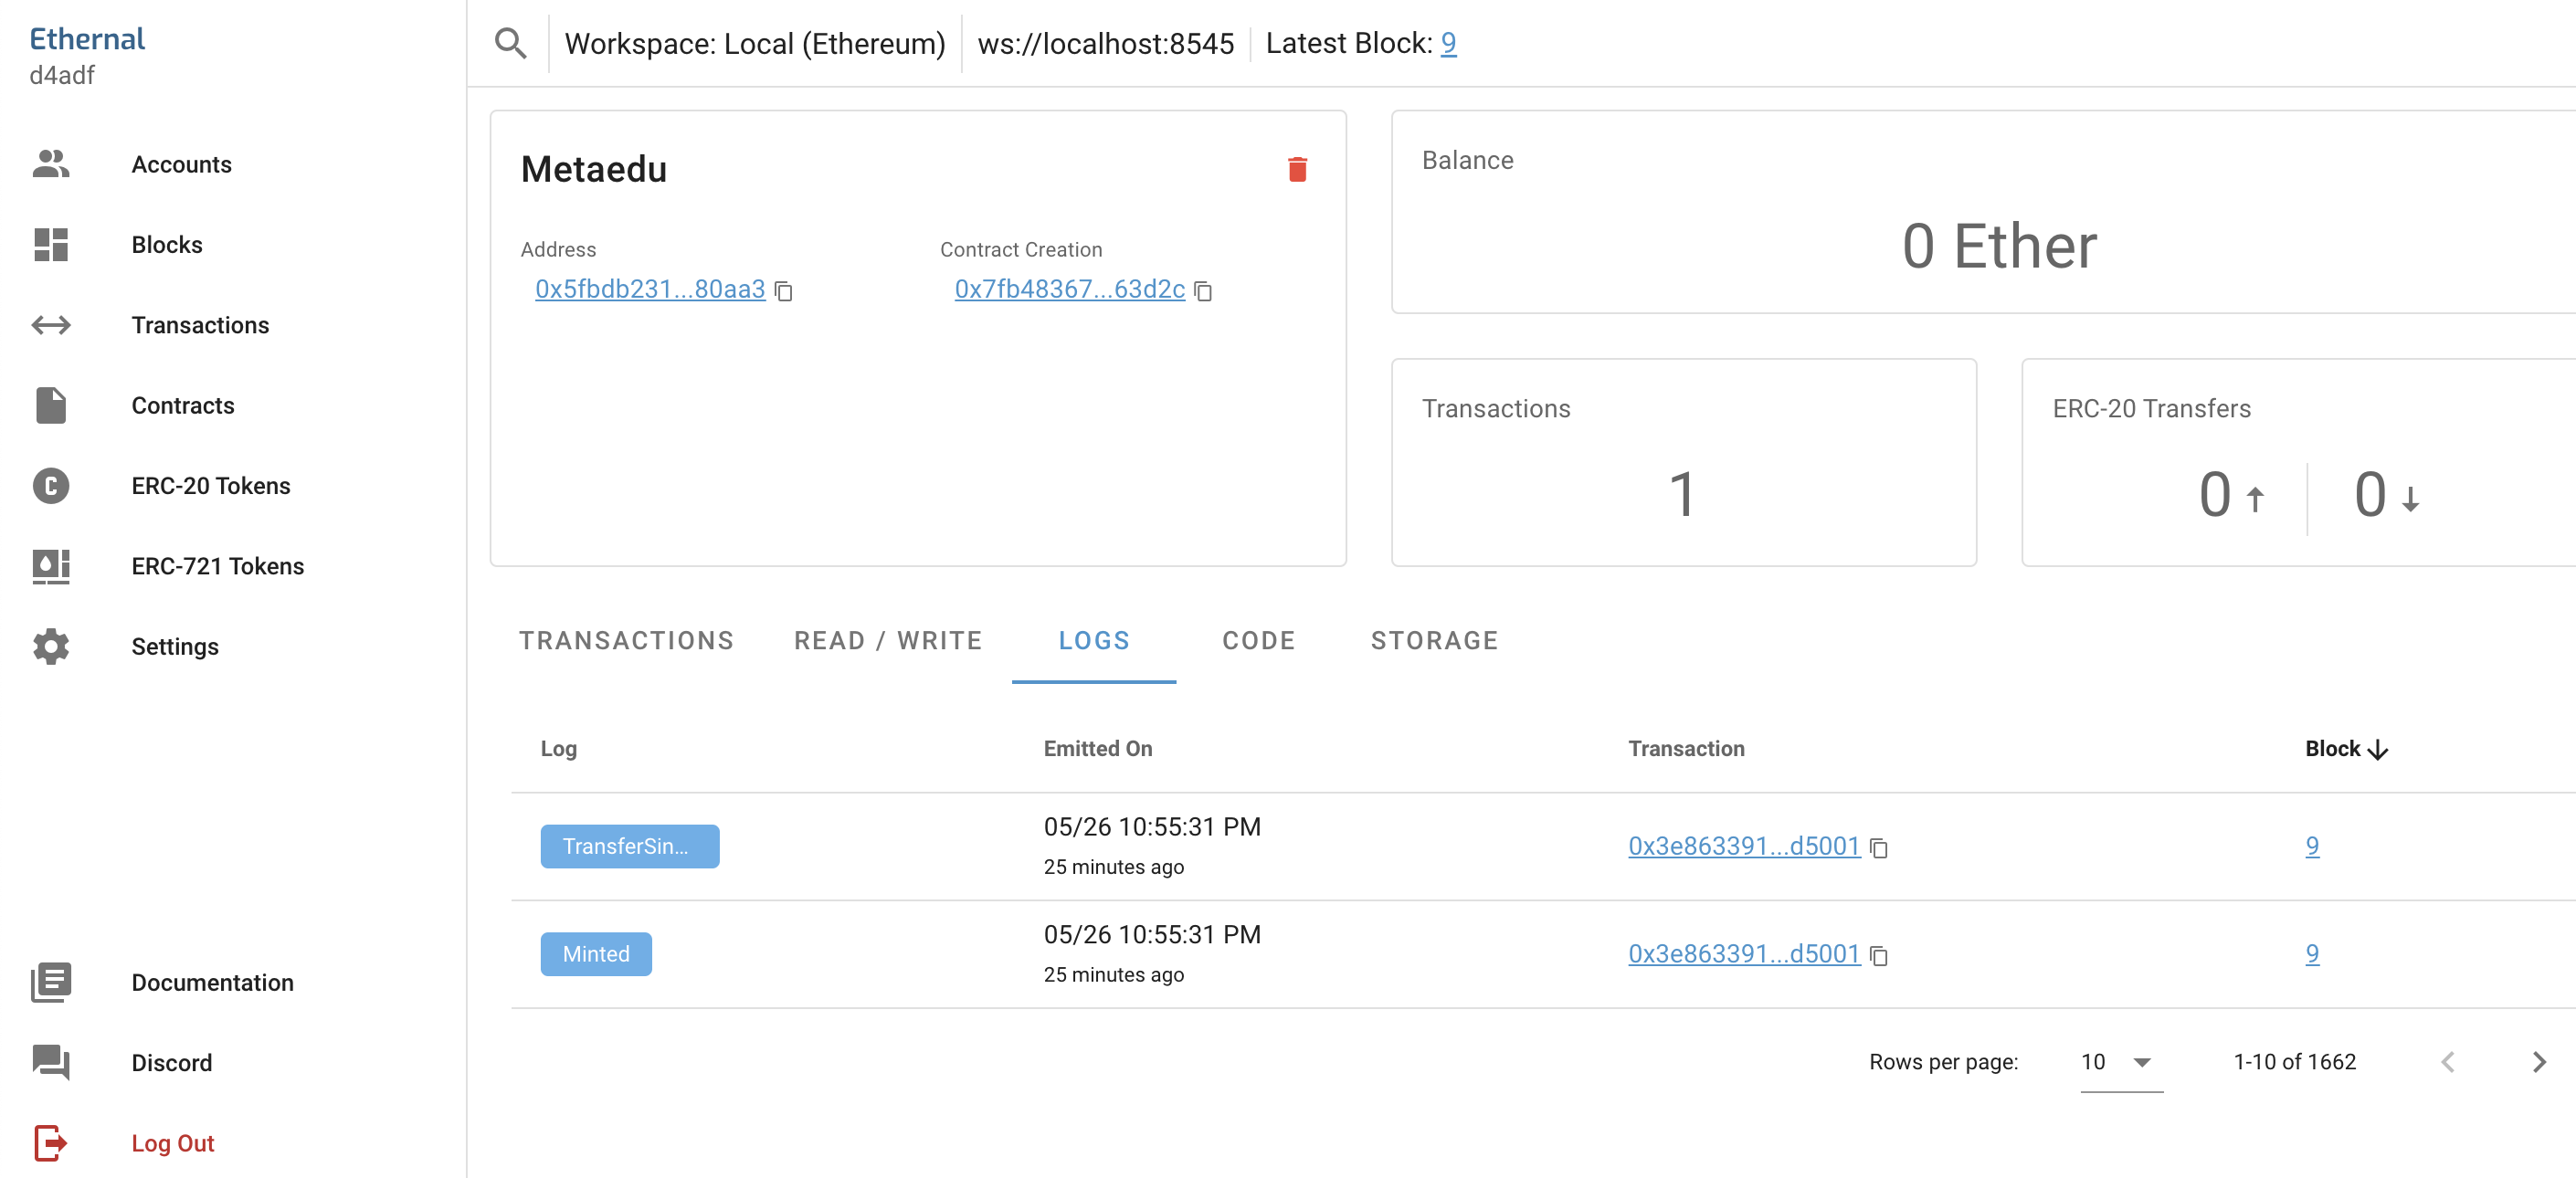
\includegraphics[scale=0.3]{gambar/img-ethernal.png}
    % Keterangan gambar yang diinputkan
    \caption{\emph{Ethernal}}
    % Label referensi dari gambar yang diinputkan
    \label{fig:Ethernal}
  \end{figure}

\subsection{\emph{Metamask}}

\emph{Metamask} adalah \emph{cold wallet} yang digunakan dalam melakukan menyimpan \emph{token}, bertransaksi dengan pengguna lain, dan berinteraksi dengan \emph{Smart Contract}. \emph{Metamask} hadir sebagai sebuah \emph{Extension} pada \emph{Browser}. Dengan menggunakan \emph{Metamask} pengguna tidak perlu memasukan \emph{Private key} setiap melakukan transaksi baik ketika membuat, menyimpan, ataupun menjual \emph{token}.

\begin{figure} [H] 
  \centering
  % Nama dari file gambar yang diinputkan
  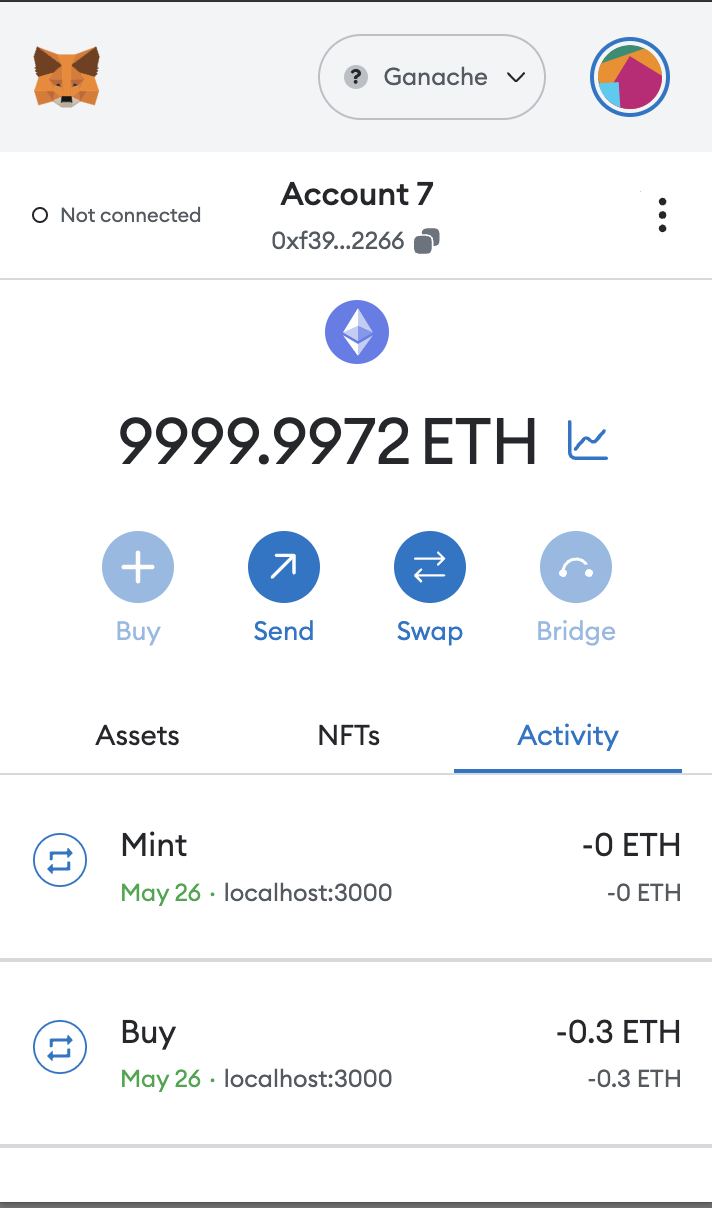
\includegraphics[scale=0.4]{gambar/img-metamask.png}
  % Keterangan gambar yang diinputkan
  \caption{\emph{Metamask}}
  % Label referensi dari gambar yang diinputkan
  \label{fig:Metamask}
\end{figure}

\section{Pengembangan \emph{Smart Contract}} 

Pada \emph{project} ini \emph{Smart Contract} dibuat untuk menjembatani dan memperoses \emph{request} dari yang dihasilkan dari interaksi pengguna ke jaringan \emph{Blockchain}. Untuk membuat \emph{NFT Marketplace} sesuai dengan \emph{Flow} yang telah ditentukan sebelumnya maka diperlukan \emph{Smart Contract} yang digunakan akan berisi berbagai \emph{variable} yang digunakan untuk menampung data-data yang dibutuhkan, \emph{function} untuk memproses data sesuai alur yang ditentukan, \emph{modifier} untuk memvalidasi parameter yang dikirim, serta \emph{event} yang digunakan untuk merekam suatu aktivitas yang terjadi pada \emph{smart contract}. 

\subsection{\emph{Variable}}

\emph{Variable} pada \emph{smart contract} berfungsi menyimpan data-data untuk kemudian diolah oleh \emph{function}. pada \emph{smart contract} ini ada beberapa \emph{variable} yang dibuat.

% Contoh pembuatan potongan kode
\begin{lstlisting}[
  language=C++,
  caption={Variable},
  label={lst:variable},
  basicstyle=\tiny,
]
  address public ownerAddress;

  Counters.Counter private tokenIds;
  mapping(uint256 => string) private uris;
  mapping(uint256 => uint256) private supplies;
  
  mapping(uint256 => mapping(address => ItemForSale)) public itemsForSale;
  mapping(uint256 => mapping(address => ItemForRent)) public itemsForRent;
  
  mapping(uint256 => uint256) private fractionsMapping;
\end{lstlisting}

\begin{itemize}
  \item \emph{ownerAddress} digunakan untuk menyimpan \emph{address} dari \emph{owner smart contract}. \emph{Variable} ini di \emph{set} ketika \emph{smart contract} di \emph{deploy}.
  \item \emph{tokenIds} digunakan untuk menyimpan index \emph{token} terakhir yang di-\emph{minting}.
  \item \emph{uris} digunakan untuk menyimpan data \emph{uri} dari setiap \emph{token} yang di-\emph{minting} dalam \emph{smart contract}. 
  \item \emph{supplies} digunakan untuk menyimpan data \emph{supply} atau jumlah dari masing-masing \emph{token}.
  \item \emph{itemsForSale} digunakan untuk menyimpan data \emph{token} yang dapat diperjual belikan.
  \item \emph{itemsForRent} digunakan untuk menyimpan data \emph{token} yang dapat disewakan.
\end{itemize}

\subsection{\emph{Event}}

\emph{Event} adalah suatu aktivitas tertentu terekam dalam \emph{Smart Contract}. Setiap pengembang dapat membuat \emph{Event}-nya sesuai dengan kebutuhan. Nantinya \emph{Event}-\emph{Event} ini dapat dilacak dan dilihat secara publik. 

% Contoh pembuatan potongan kode
\begin{lstlisting}[
  language=C++,
  caption={Program halo dunia.},
  label={lst:halodunia},
  basicstyle=\tiny,
]
event Minted(
  uint256 indexed tokenId,
  string uri,
  address indexed owner,
  address indexed nftAddress,
  uint256 supply
);
event ShareOwnership(
  uint256 indexed tokenId,
  address indexed owner,
  uint256 supply
);
event ItemAddedForSale(
  uint256 tokenId,
  address owner,
  uint256 supply,
  uint256 price
);
event ItemAddedForRent(
  uint256 tokenId,
  address owner,
  uint256 supply,
  uint256 price
);
event ItemBuy(
  address buyer,
  address seller,
  uint256 tokenId,
  uint256 price
); 
event ItemRent(
  address user,
  address owner,
  uint256 tokenId,
  uint256 price,
  uint256 day
); 
\end{lstlisting}

\begin{itemize}
  \item \emph{Minted} adalah aktivitas yang digunakan untuk menandai bahwa terdapat \emph{token} baru yang di-\emph{minting}.
  \item \emph{ShareOwnership} adalah aktivitas yang digunakan untuk menanandai bahwa terdapat \emph{NFT} yang di-\emph{fraction}.
  \item \emph{ItemAddedForSale} adalah aktivitas yang digunakan untuk menandai bahwa terdapat \emph{token} yang dapat diperjual belikan.
  \item \emph{ItemAddedForRent} adalah aktivitas yang digunakan untuk menandai bahwa terdapat \emph{token} yang dapat disewakan.
  \item \emph{ItemBuy} adalah aktivitas yang digunakan untuk menandai bahwa terdapat \emph{token} yang dibeli. 
  \item \emph{ItemRent} adalah aktivitas yang digunakan untuk menandadi bahwa terdapat \emph{token} yang disewa.
\end{itemize}

\subsection{\emph{Modifier}}

\emph{Modifier} adalah \emph{block code} yang digunakan untuk memvalidasi parameter yang diberikan dalam pemanggilan \emph{function} tertentu. \emph{Modifier} memastikan bahwa segala parameter telah valid sebelum diproses oleh suatu \emph{function}.

% Contoh pembuatan potongan kode
\begin{lstlisting}[
  language=C++,
  caption={Modifier},
  label={lst:modifier},
  basicstyle=\tiny,
]
modifier ItemIsNonFungible(uint256 _tokenId) {
  require(supplies[_tokenId] == 1, "Token is fungible");
}

modifier ItemIsAvailableForBuy(uint256 _tokenId, address _seller) {
  require(
      itemsForSale[_tokenId][_seller].isSold == false,
      "Token is sold"
  );
}

modifier ItemIsAvailableForRent(
  uint256 _tokenId,
  address _seller,
  uint256 datetime
) {
  require(
      itemsForRent[_tokenId][_seller].expirationTime <= datetime ||
          itemsForRent[_tokenId][_seller].expirationTime == 0,
      "Token is rented"
  );
}

modifier BuyerIsValid(uint256 _tokenId, address _seller) {
  require(msg.sender != _seller, "Buyer is not valid");
}

modifier UserIsValid(uint256 _tokenId, address _owner) {
  require(msg.sender != _owner, "Buyer is not valid");
}

modifier AmountForBuyIsValid(uint256 _price) {
  require(msg.value >= _price * 1000000000000, "Amount is not valid");
}

modifier AmountForRentIsValid(uint256 _price) {
  require(msg.value >= _price * 1000000000000, "Amount is not valid");
}

modifier ItemIsAvailableForSale(uint256 _tokenId, uint256 _supply) {
  uint256 itemSupply = balanceOf(msg.sender, _tokenId);
  uint256 sellItemSupply = itemsForSale[_tokenId][msg.sender].supply;
  uint256 availableItemSupply = itemSupply - sellItemSupply;
  require(
      availableItemSupply > _supply,
      "Item is not available for sale"
  );
}

modifier ItemIsNotInRentalPeriod(
  uint256 _tokenId,
  address _owner,
  uint256 _datetime
) {
  require(
      itemsForRent[_tokenId][_owner].expirationTime < _datetime,
      "Item is in rental period"
  );
}
\end{lstlisting}

\begin{itemize}
  \item \emph{ItemIsNonFungible} digunakan untuk memvalidasi bahwa \emph{token} merupakan \emph{NFT}.
  \item \emph{ItemIsAvailableForBuy} digunakan untuk memvalidasi bahwa \emph{token} dapat dibeli.
  \item \emph{ItemIsAvailableForRent} digunakan untuk memvalidasi bahwa \emph{token} dapat disewa.
  \item \emph{BuyerIsValid} digunakan untuk memvalidasi bahwa pembeli memiliki \emph{address} yang berbeda dengan \emph{seller} \emph{token}.
  \item \emph{UserIsValid} digunakan untuk memvalidasi bahwa penyewa memiliki \emph{address} yang berbeda dengan \emph{owner} \emph{token}.
  \item \emph{AmountForBuyIsValid} digunakan untuk memvalidasi bahwa \emph{ether} yang dikirim sesuai dengan harga dari \emph{token} yang dibeli.
  \item \emph{AmountForRentIsValid} digunakan untuk memvalidasi bahwa \emph{ether} yang dikirim sesuai dengan harga sewa dari \emph{token}.
  \item \emph{ItemIsNotInRentalperiod} digunakan untuk memvalidasi bahwa \emph{token} tidak sedang dalam masa penyewaan.
\end{itemize}

\subsection{\emph{Function}}

\emph{Function} adalah \emph{block code} berisi \emph{logic} untuk memperoses data sesuai dengan \emph{business logic} yang telah ditentutkan. \emph{Function}-\emph{function} utama dalam \emph{smart contract} yang dikembangkan diantaranya adalah \emph{mint}, \emph{putItemForSale}, \emph{putItemForRent}, \emph{buy}, \emph{rent}, \emph{shareOwnership}

\subsubsection{\emph{Mint}}

% Contoh pembuatan potongan kode
\begin{lstlisting}[
  language=C++,
  caption={Mint},
  label={lst:mint},
  basicstyle=\tiny,
]
function mint(
  uint256 _supply,
  string memory _uri
) public {
  tokenIds.increment();
  uint256 tokenId = tokenIds.current();
  _mint(msg.sender, tokenId, _supply, "");
  uris[tokenId] = _uri;
  supplies[tokenId] = _supply;
  emit Minted(tokenId, _uri, msg.sender, address(this), _supply);
}
\end{lstlisting}

\emph{Function} \emph{mint} digunakan untuk mendaftarkan \emph{token} baru dimana proses ini biasa dikenal sebagai \emph{minting}. Parameter pada funsi ini adalah \emph{supply} yang berisi jumlah \emph{token} yang beredar. Jika nilai \emph{supply} yang dikirimkan adalah 1 maka \emph{token} tersebut adalah NFT sebaliknya jika lebih dari 1 maka \emph{token} tersebut adalah \emph{token fungible}.

\subsubsection{\emph{PutItemForSale}}

% Contoh pembuatan potongan kode
\begin{lstlisting}[
  language=C++,
  caption={Mint},
  label={lst:mint},
  basicstyle=\tiny,
]
function putItemForSale(
  uint256 _tokenId,
  uint256 _price,
  uint256 _supply,
  uint256 _datetime
)
  external
  ItemIsNotInRentalPeriod(_tokenId, msg.sender, _datetime)
  OwnerIsValid(_tokenId)
{
  itemsForSale[_tokenId][msg.sender] = ItemForSale({
      tokenId: _tokenId,
      supply: _supply,
      seller: payable(msg.sender),
      price: _price,
      isSold: false
  });
  emit ItemAddedForSale(_tokenId, msg.sender, _supply, _price);
}
\end{lstlisting}

\emph{Function} \emph{putItemForSale} supaya pemilik \emph{token} dapat menjual \emph{token} yang dimiliki. \emph{Function} ini perlu dipanggil apabila pemilik menghendaki untuk menjual dikarenakan \emph{token} yang baru saja di-\emph{minting} tidak dapat langsung diperjual belikan.

\subsubsection{\emph{PutItemForRent}}

% Contoh pembuatan potongan kode
\begin{lstlisting}[
  language=C++,
  caption={Rent},
  label={lst:rent},
  basicstyle=\tiny,
]
function putItemForRent(
  uint256 _tokenId,
  uint256 _price,
  uint256 _supply,
  uint256 _datetime
)
  external
  ItemIsNotInRentalPeriod(_tokenId, msg.sender, _datetime)
  OwnerIsValid(_tokenId)
  ItemIsNonFungible(_tokenId)
{
  itemsForRent[_tokenId][msg.sender] = ItemForRent({
      tokenId: _tokenId,
      supply: _supply,
      owner: payable(msg.sender),
      user: msg.sender,
      price: _price,
      expirationTime: 0
  });
  emit ItemAddedForRent(_tokenId, msg.sender, _supply, _price);
}
\end{lstlisting}

\emph{Function} \emph{putItemForRent} supaya pemilik \emph{token} dapat menyewakan \emph{token} yang dimiliki. \emph{Function} ini perlu dipanggil apabila pemilik menghendaki untuk menyewakan \emph{token}-nya dikarenakan \emph{token} yang baru saja di-\emph{minting} tidak dapat langsung disewakan.

\subsubsection{\emph{Buy}}

% Contoh pembuatan potongan kode
\begin{lstlisting}[
  language=C++,
  caption={Buy},
  label={lst:buy},
  basicstyle=\tiny,
]
function buy(
  uint256 _tokenId,
  uint256 _quantity,
  address payable _seller,
  uint256 _datetime
)
  external
  payable
  BuyerIsValid(_tokenId, _seller)
  ItemIsNotInRentalPeriod(_tokenId, _seller, _datetime)
  AmountForBuyIsValid(itemsForSale[_tokenId][_seller].price)
  ItemIsAvailableForBuy(_tokenId, _seller)
{
  safeTransferFrom(_seller, msg.sender, _tokenId, _quantity, "0x0");
  itemsForSale[_tokenId][_seller].isSold = true;
  _seller.transfer(msg.value);
}
\end{lstlisting}

\emph{Function} \emph{buy} digunakan untuk memproses \emph{request}  pembelian \emph{token} oleh user.

\subsubsection{\emph{Rent}}

% Contoh pembuatan potongan kode
\begin{lstlisting}[
  language=C++,
  caption={Rent},
  label={lst:rent},
  basicstyle=\tiny,
]
function rent(
  uint256 _tokenId,
  uint256 _day,
  address payable _owner,
  uint256 _datetime
)
  external
  payable
  ItemIsNotInRentalPeriod(_tokenId, _owner, _datetime)
  UserIsValid(_tokenId, _owner)
  AmountForRentIsValid(itemsForRent[_tokenId][_owner].price * _day)
  ItemIsAvailableForRent(_tokenId, _owner, _datetime)
{
  itemsForRent[_tokenId][_owner].expirationTime = (_day * 86400000)+_datetime;
  itemsForRent[_tokenId][_owner].user = msg.sender;
  _owner.transfer(msg.value);
}
\end{lstlisting}

\emph{Function} \emph{rent} digunakan untuk memproses \emph{request} penyewaan \emph{token} yang belum di-\emph{fraction} oleh \emph{owner} dari \emph{token} tersebut.

\subsubsection{\emph{RentFraction}}

% Contoh pembuatan potongan kode
\begin{lstlisting}[
  language=C++,
  caption={RentFraction},
  label={lst:rentFraction},
  basicstyle=\tiny,
]
function rentFraction(
        uint256 _tokenId,
        uint256 _day,
        address payable[] memory _ownerList,
        uint256[] memory _shareList,
        uint256 _datetime
    )
        external
        payable
        ItemIsNotInRentalPeriod(_tokenId, ownerAddress, _datetime)
        UserIsValid(_tokenId, ownerAddress)
        AmountForRentIsValid(itemsForRent[_tokenId][ownerAddress].price * _day)
        ItemIsAvailableForRent(_tokenId, ownerAddress, _datetime)
    {
        ItemForRent memory itemForRent = itemsForRent[_tokenId][ownerAddress];
        itemForRent.expirationTime = (_day * 86400000) + _datetime;
        itemForRent.user = msg.sender;
        for (uint256 i = 0; i < _ownerList.length; i++) {
            if (
                balanceOf(_ownerList[i], fractionsMapping[_tokenId]) ==
                _shareList[i]
            ) {
                _ownerList[i].transfer(
                    (msg.value * _shareList[i]) /
                        supplies[fractionsMapping[_tokenId]]
                );
            }
        }
    }
\end{lstlisting}

\emph{Function} \emph{rentFraction} digunakan untuk memproses \emph{request} penyewaan \emph{token} yang telah di-\emph{fraction} oleh \emph{owner} dari \emph{token} tersebut. Perbedaan dari \emph{function} \emph{rent} sebelumnya adalah \emph{function} ini membagikan \emph{ether} yang dikirim kepada seluruh \emph{address} yang memiliki \emph{token} hasil \emph{fraction} sebanding dengan jumlah kepemilikannya.

\section{Penyiapan \emph{Database}}

\emph{Database} adalah kumpulan dari data-data yang dikelola berdasarkan sedemikan rupa berdasarkan ketentuan tertentu. Pada \emph{project} \emph{NFT Marketplace} ini digunakan untuk menyimpan berbagai data seperti data \emph{user}, \emph{token}, \emph{ownership}, \emph{rental}, \emph{fraction}, dan \emph{transaction}. Data-data ini juga disimpan pada \emph{Blockchain}, akan tetapi untuk mayoritas proses pengambilan data akan diperoleh dari \emph{database} supaya dapat memberikan kecepatan pemrosesan yang lebih cepat. Database yang digunakan adalah \emph{PostgreSQL} hal ini dikarenakan \emph{PostgreSQL} mampu memberikan keamanan dalam pemprosesan suatu transaksi dikarenakan telah \emph{comply} dengan prinsip \emph{ACID} (\emph{Atomicity, Consistency, Isolation, and Durability}). Hal ini menjadi penting untuk menghindari kerusakan data akibat adanya kegagalan sistem ketika transaksi antar \emph{user} sedang diproses. Selain itu, walaupun PostgreSQL merupakan \emph{SQL} (Structured query language), \emph{database} ini juga mampu menyimpan data yang \emph{semi-unstructured} seperti \emph{JSON} \emph{(JavaScript Object Notation)} yang digunakan untuk menyimpan \emph{metadata} \emph{token}.

\begin{figure} [H] \centering
  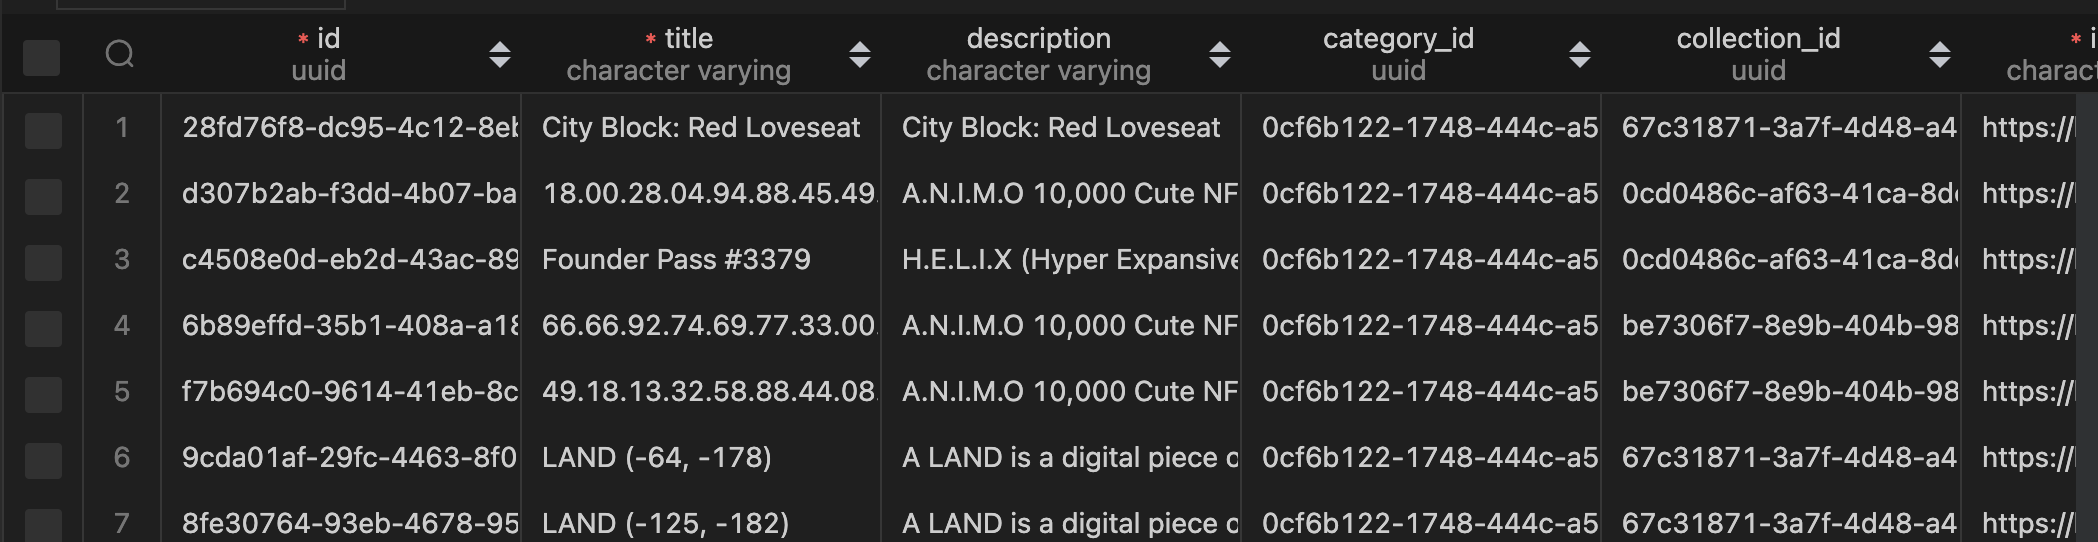
\includegraphics[scale=0.35]{gambar/img-table-tokens.png}
  \caption{Tabel \emph{token}}
  \label{fig:TokenTable}
\end{figure}

Digunakan untuk menyimpan data \emph{token} seperti nama, deskripsi, kategori, koleksi dan lainnya terkait dengan suatu \emph{token}.

\begin{figure} [H] \centering
  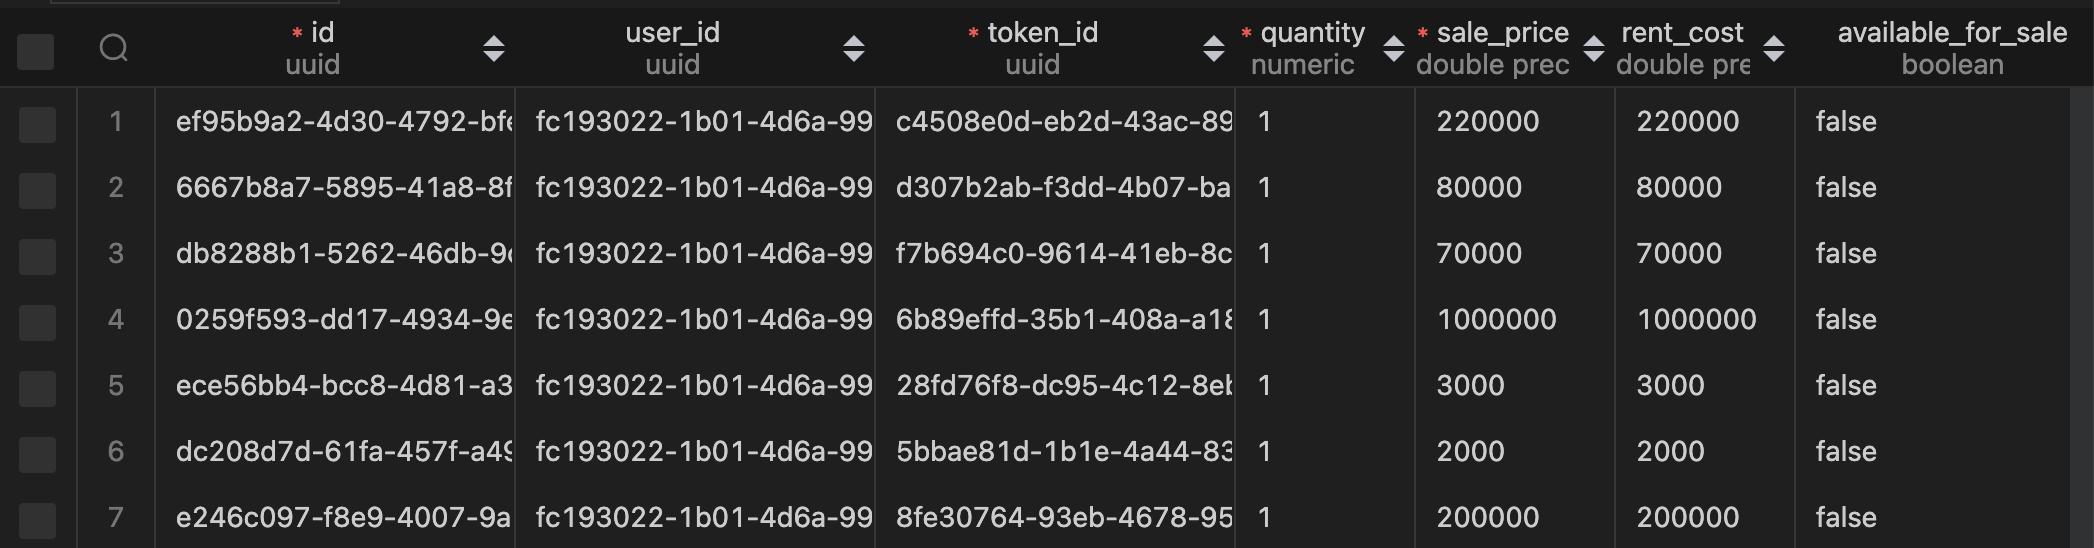
\includegraphics[scale=0.35]{gambar/img-table-ownerships.png}
  \caption{Tabel \emph{ownerships} }
  \label{fig:OwnershipTable}
\end{figure}

Digunakan untuk menyimpan data kepemilikan suatu token oleh pengguna meliputi id token, id pengguna, jumlah kepemilikan, status penjualan, dan status penyewaan.

\begin{figure} [H] \centering
  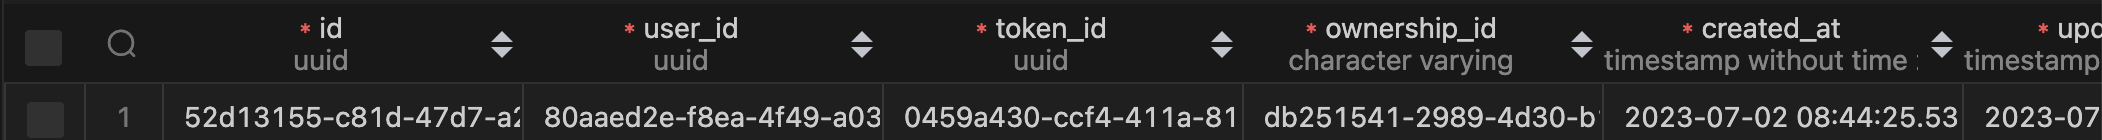
\includegraphics[scale=0.35]{gambar/img-table-rentals.png}
  \caption{Tabel \emph{rentals}}
  \label{fig:OwnershipTable}
\end{figure}

Digunakan untuk menyimpan data penyewaan suatu token oleh pengguna meliputi id token, id kepemilikan, id pengguna, dan lama penyewaan.

\begin{figure} [H] \centering
  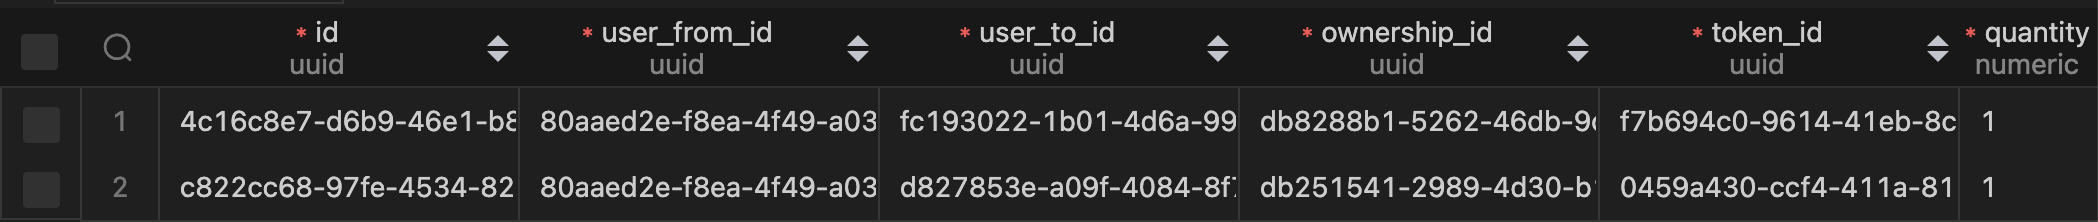
\includegraphics[scale=0.35]{gambar/img-table-transactions.png}
  \caption{Tabel \emph{rentals}}
  \label{fig:TransactionsTable}
\end{figure}

Digunakan untuk menyimpan data transaksi baik penjualan maupun penyewaan yang meliputi id pembeli, id penjual, id token, dan jumlah token yang dijual.

\begin{figure} [H] \centering
  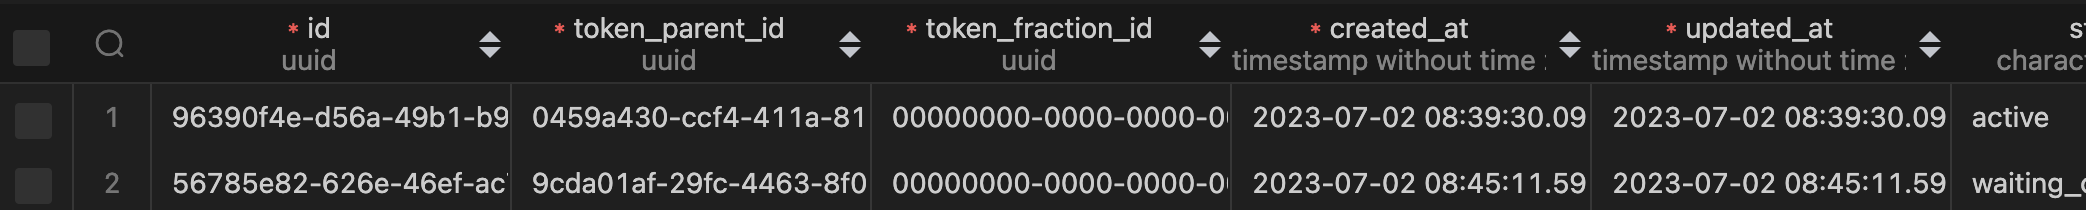
\includegraphics[scale=0.35]{gambar/img-table-fractions.png}
  \caption{Tabel \emph{fractions}}
  \label{fig:FractionsTable}
\end{figure}

Digunakan untuk menyimpan data \emph{fractionilalizations} suatu token hasil proses \emph{share ownership} oleh pengguna meliputi id token asal, id token pencahan, dan id pengguna.

\section{Pengembangan \emph{Back End}} 

\emph{Back End} adalah bagian dari aplikasi yang tidak terlihat oleh pengguna yang memproses seluruh data ketika \emph{request} dikirimkan oleh \emph{user}. Aplikasi \emph{Back End} dikembangkan menggunakan bahasa pemrograman \emph{Golang}. \emph{Golang} dipilih dikarenakan memiliki performat yang lebih cepat dari banyak bahasa pemrograman lain. Hal tersebut dikarenakan \emph{Golang} adalah \emph{Compiled language} bukan \emph{Interpreted language} sehingga dapat langsung dibaca oleh mesin. Selain itu \emph{Golang} juga memiliki fitur \emph{multithread} sehingga akan memaksimalkan potensi dari \emph{Server} yang digunakan. Aplikasi \emph{Back End} akan mengambil data dari \emph{Database} yang dalam hal ini adalah \emph{PostgreSQL} dan juga \emph{Redish} sebagai tempat penyimpanan \emph{Cache}. Ketika data yang butuhkan oleh \emph{user} tidak ada di \emph{Redish} maka \emph{aplikasi} akan mengambil data dari \emph{Database} kemudian data tersebut aplikasi melakukan proses \emph{write} \emph{cache} pada \emph{Redis} sehingga jika ada \emph{user} lain memerlukan data yang sama tidak perlu mengambil data kembali dari \emph{Database}.

Aplikasi \emph{Back End} yang dikembangkan berupa \emph{API} (\emph{Application Programming Interdace}) yang nantinya akan diakses oleh \emph{frontend} dan \emph{platform metaverse} melalui protokol \emph{HTTP/HTTPS}. 

\section{Pengembangan \emph{Front End}} 

\emph{Front End} adalah bagian dari aplikasi yang terlihat dan menjadi tempat berinteraksi \emph{user}. Pada pengembangan \emph{project} \emph{NFT Marketplace} ini dipilih \emph{NextJS} sebagai \emph{framework}-nya. \emph{NextJS} dipilih dikarenakan memiliki fitur \emph{server side rendering}. Hal ini berarti \emph{Server} mampu menghasilkan \emph{HTML} untuk sebuah halaman dan mengirimkannya langsung kepada \emph{client}. Sebaliknya \emph{framework} lain layaknya \emph{ReactJS} mengirimkan \emph{Javascript} kepada \emph{Client} kemudian \emph{Client} sendiri lah yang akan memproses nya untuk memperoleh \emph{HTML}. Dengan fitur tersebut mampu meningkatkan aspek \emph{SEO} dari \emph{web} yang dikembangkan. Selain itu pengembangan aplikasi \emph{Front End} juga dikolaborasikan dengan \emph{framework} lain seperti \emph{tailwind} dan \emph{AntDesign} untuk memberikan tampilan yang lebih konsisten.  


\cleardoublepage

% Bab 4 pengujian dan analisis
\chapter{HASIL DAN PEMBAHASAN}
\label{chap:pengujiananalisis}

Pada bab ini akan dipaparkan hasil pengerjaan tugas akhir berupa \emph{Web NFT Marketplace}, \emph{API}, \emph{Smart Contract}, dan \emph{Metaverse}. 

Hasil penelitian adalah sebagai berikut:

\subsection{\emph{Web NFT Marketplace}}
\label{sec:webnftmarketplace}

\subsection{Halaman Awal \emph{NFT Marketplace}} 

\begin{figure} [H] \centering
  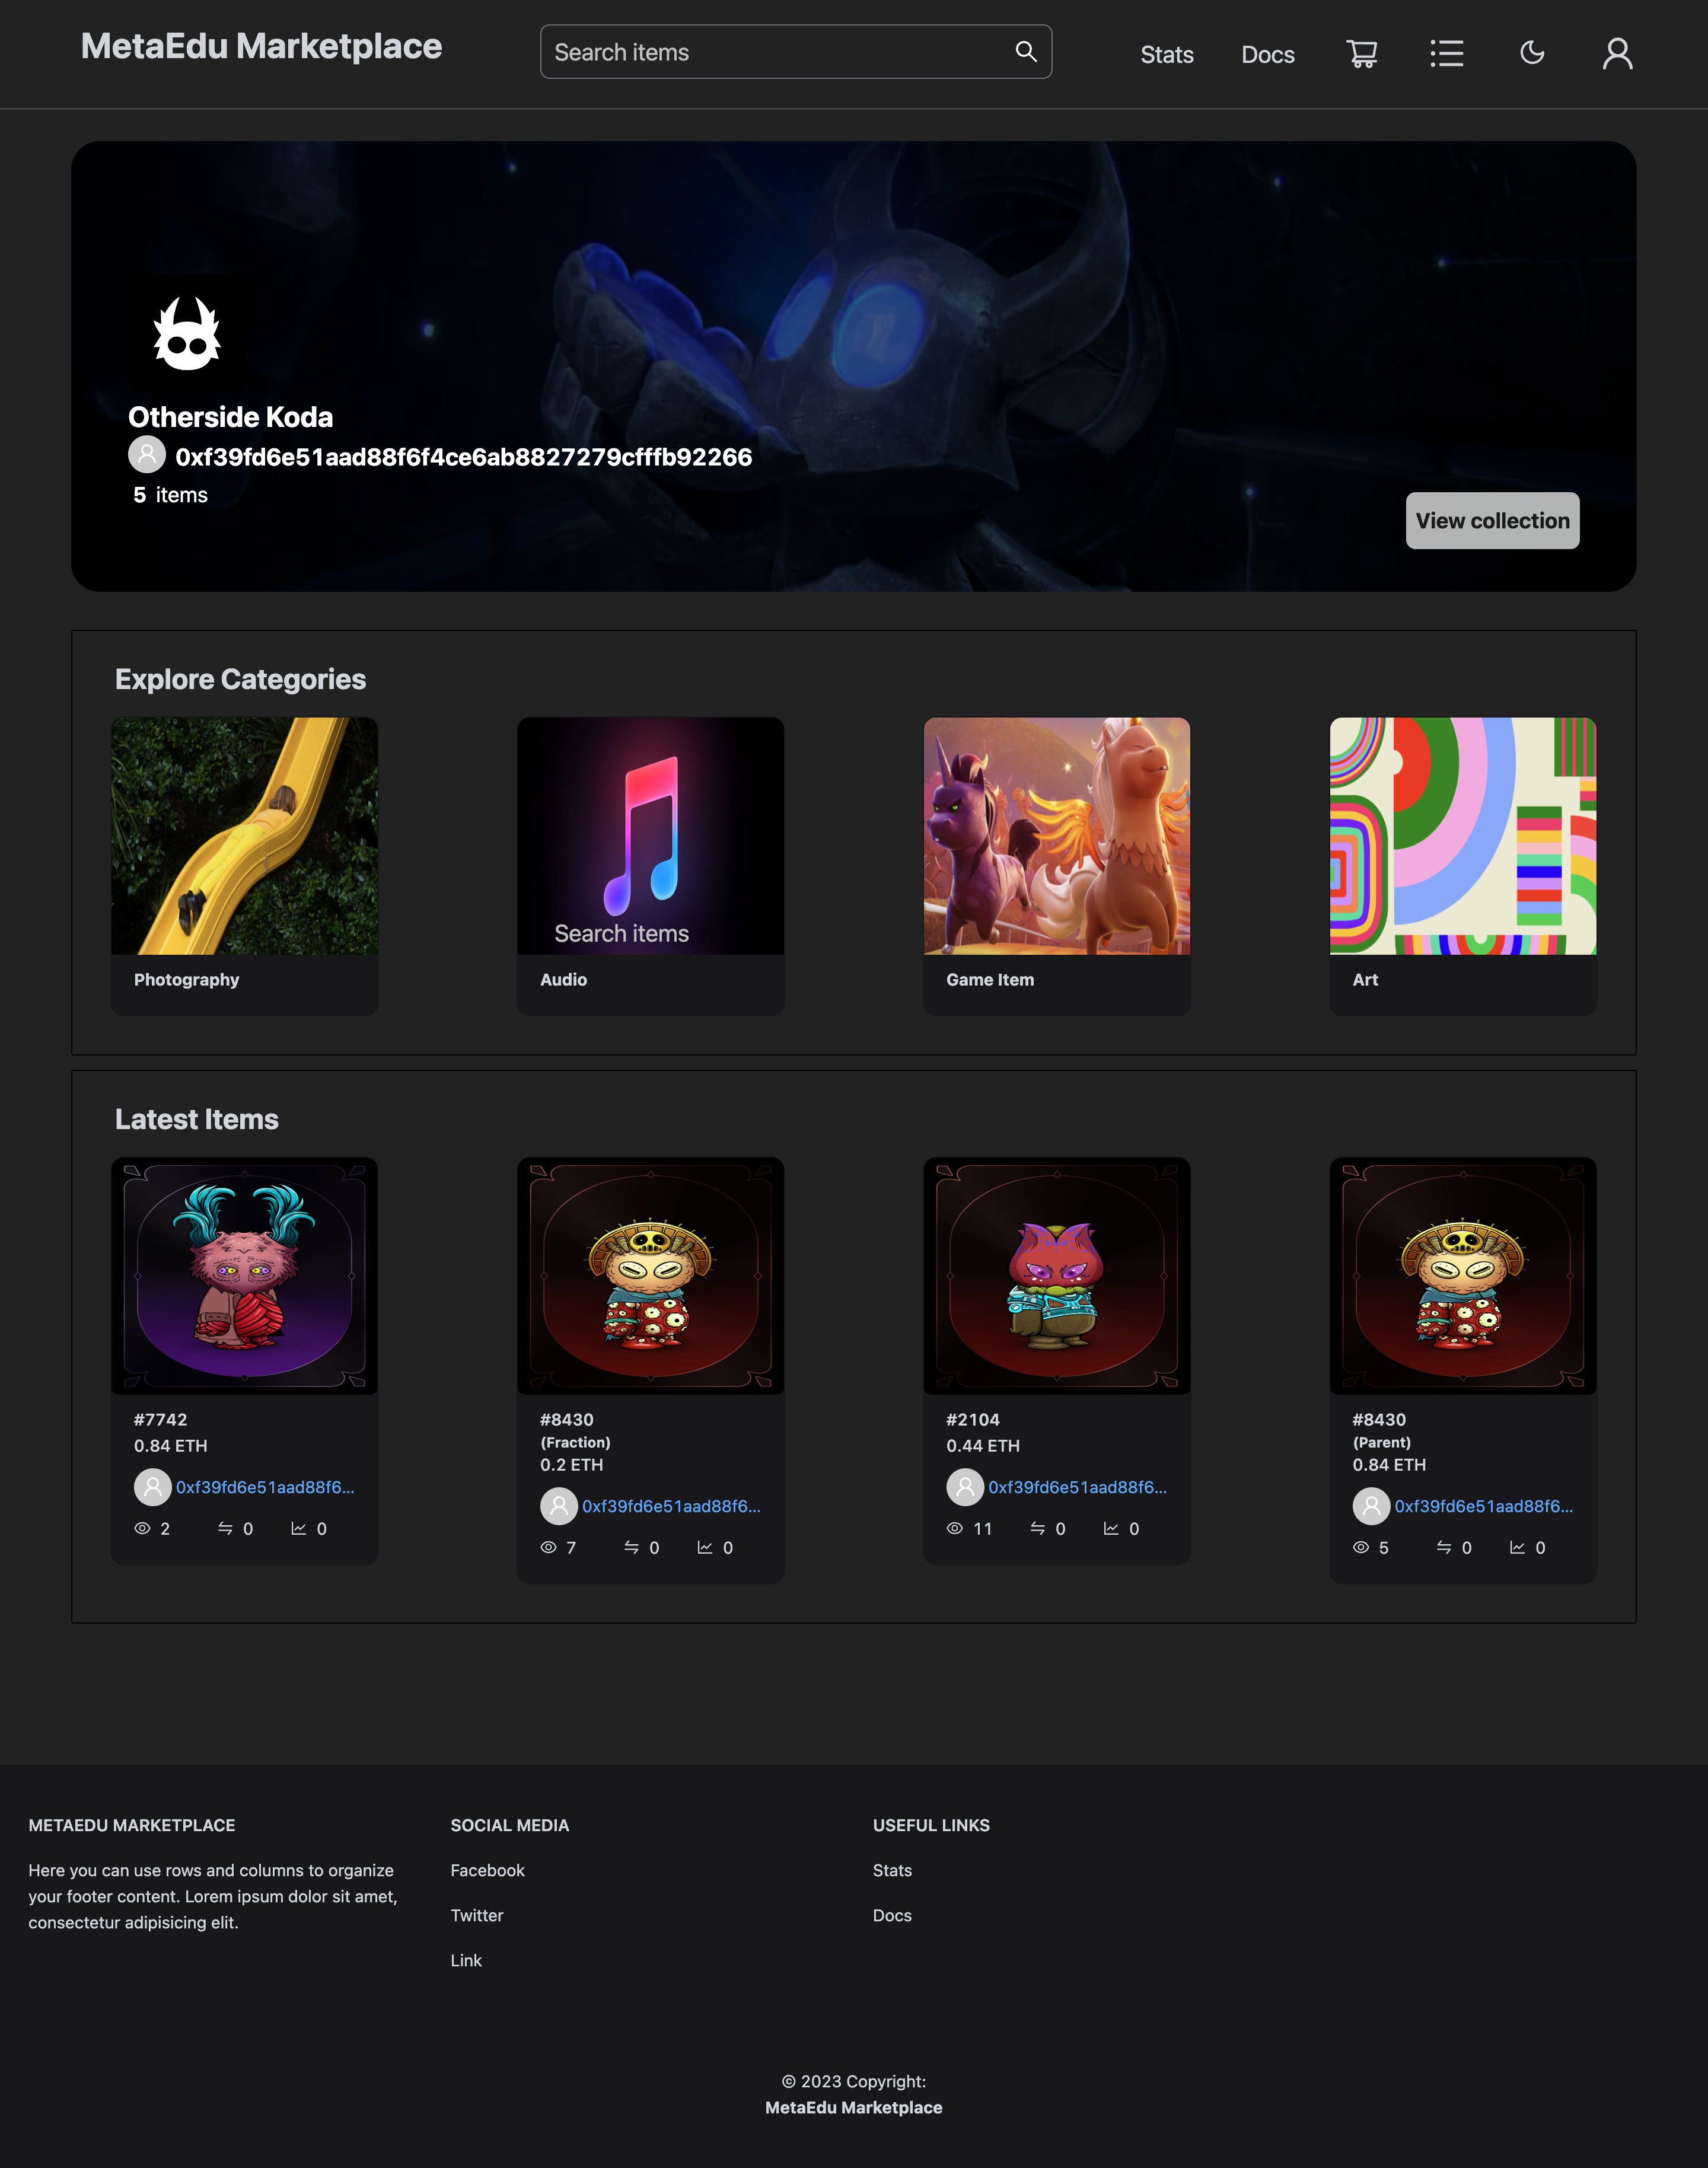
\includegraphics[scale=0.12]{gambar/img-frontend-index.png}
  \caption{Halaman awal \emph{NFT Marketplace}}
  \label{fig:NFTMarketplace}
\end{figure}

Tampilan awal \emph{NFT Marketplace}, menampilkan koleksi \emph{token}, kategori \emph{token}, dan \emph{token} terbaru.

\subsection{Halaman \emph{Minting Token}}

\begin{figure} [H] \centering
  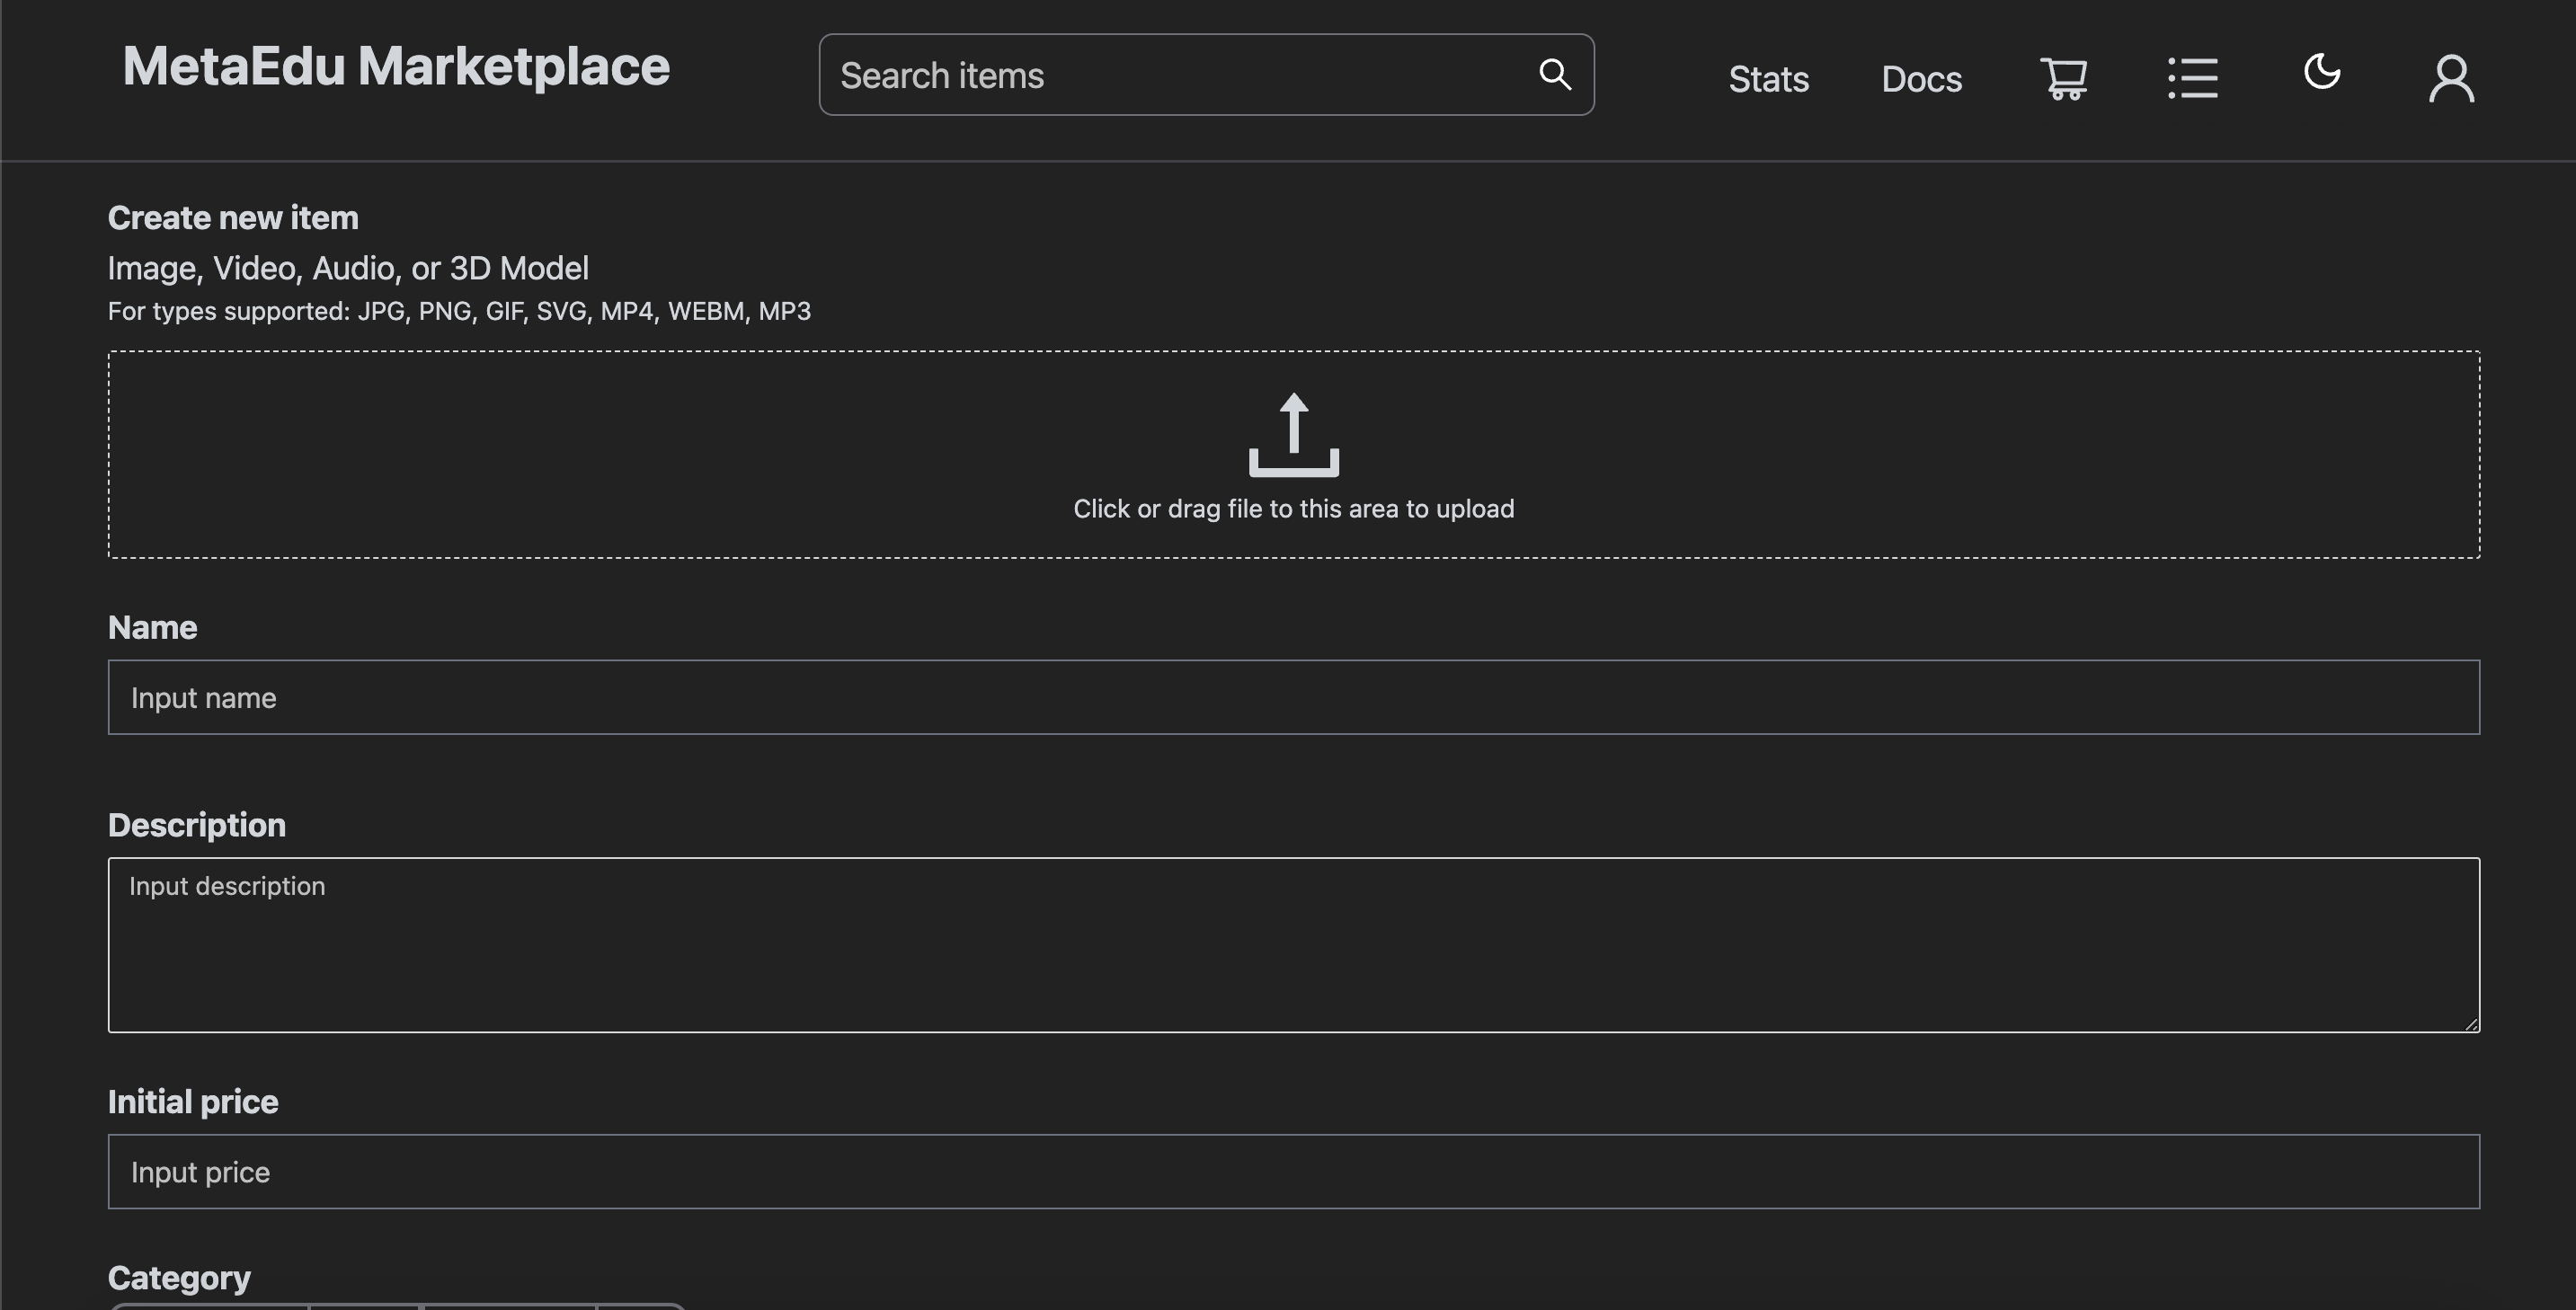
\includegraphics[scale=0.3]{gambar/img-frontend-add-token.png}
  \caption{Halaman \emph{Minting Token}}
  \label{fig:TokenMinting}
\end{figure}

Halaman \emph{Minting token} merupakan halaman yang digunakan \emph{user} untuk membuat \emph{token} baru. Untuk membuat \emph{token} baru, \emph{user} perlu memasukan \emph{image} \emph{token}, nama \emph{token}, harga awal, suplai, dan koleksi. 

\subsection{Halaman Detail \emph{Token}}

\begin{figure} [H] \centering
  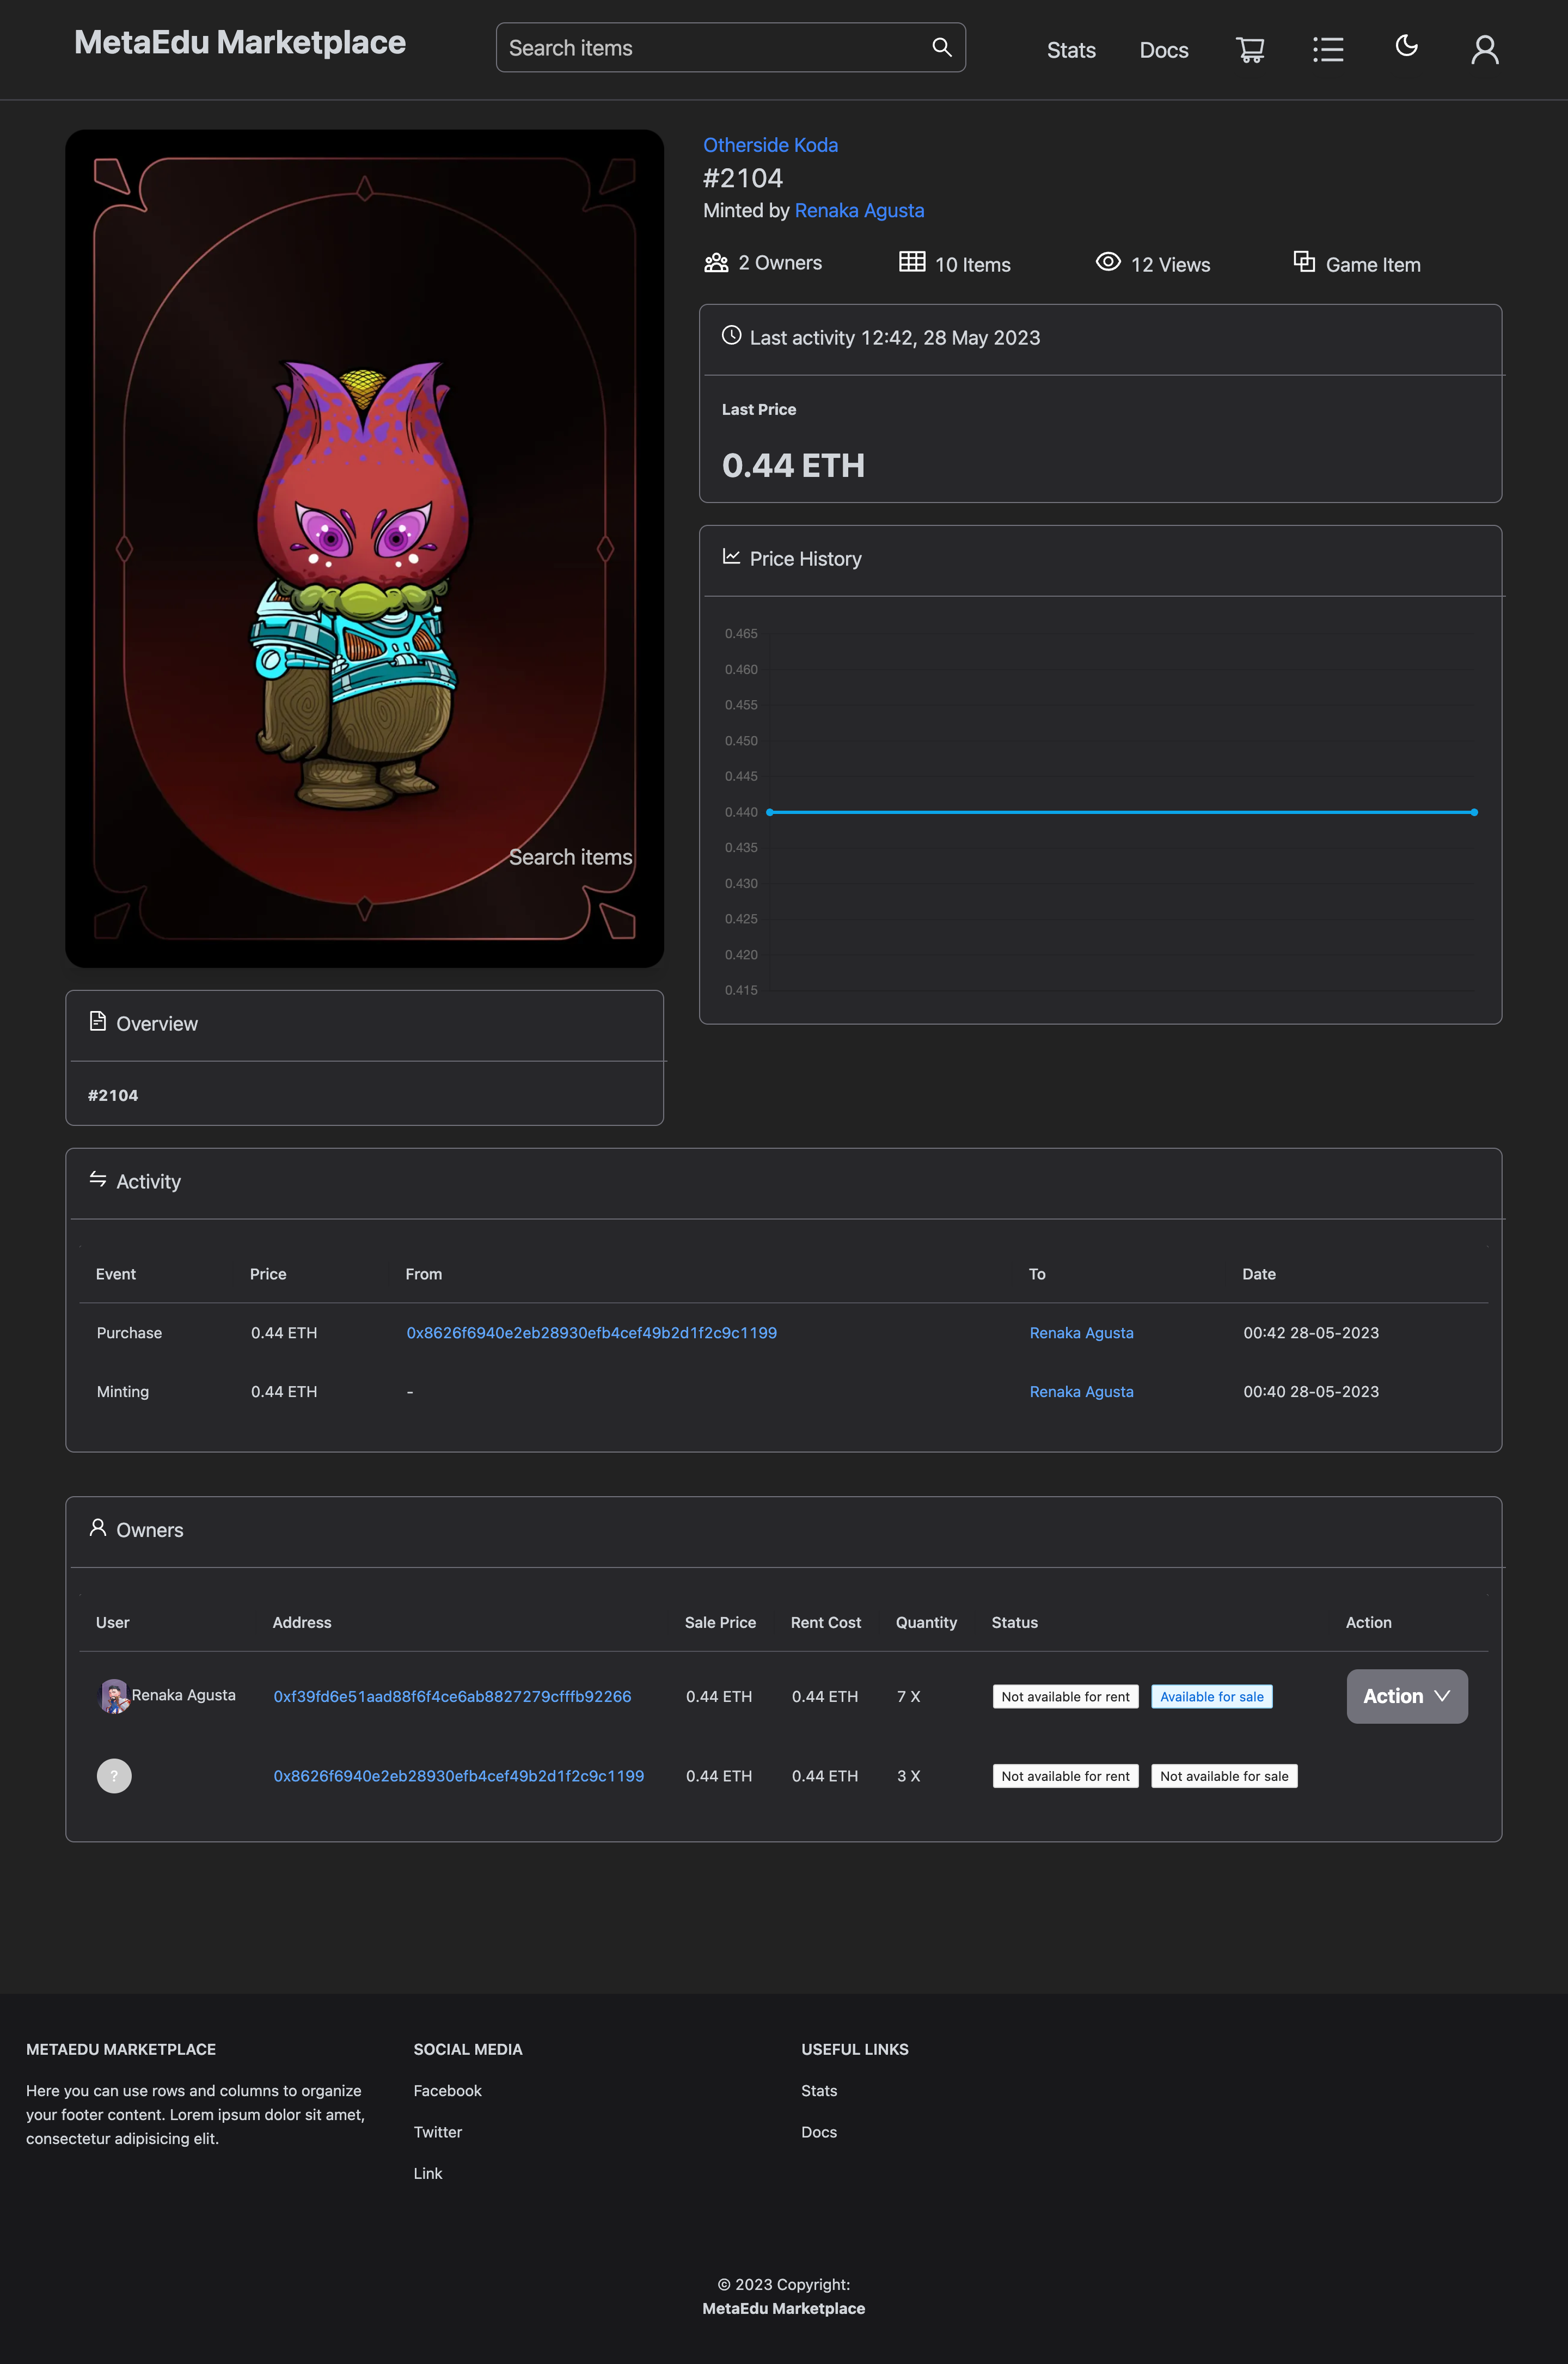
\includegraphics[scale=0.1]{gambar/img-frontend-token-detail.png}
  \caption{Halaman detail \emph{Token}}
  \label{fig:TokenDetail}
\end{figure}

Halaman detail \emph{token} menampilkan informasi-informasi mengenai nama \emph{token}, harga terakhir, pergerakan harga, riwayat transaksi, daftar kepemilkan dan lainnya. 

\subsection{Halaman Pencarian \emph{Token}}
\begin{figure} [H] \centering
  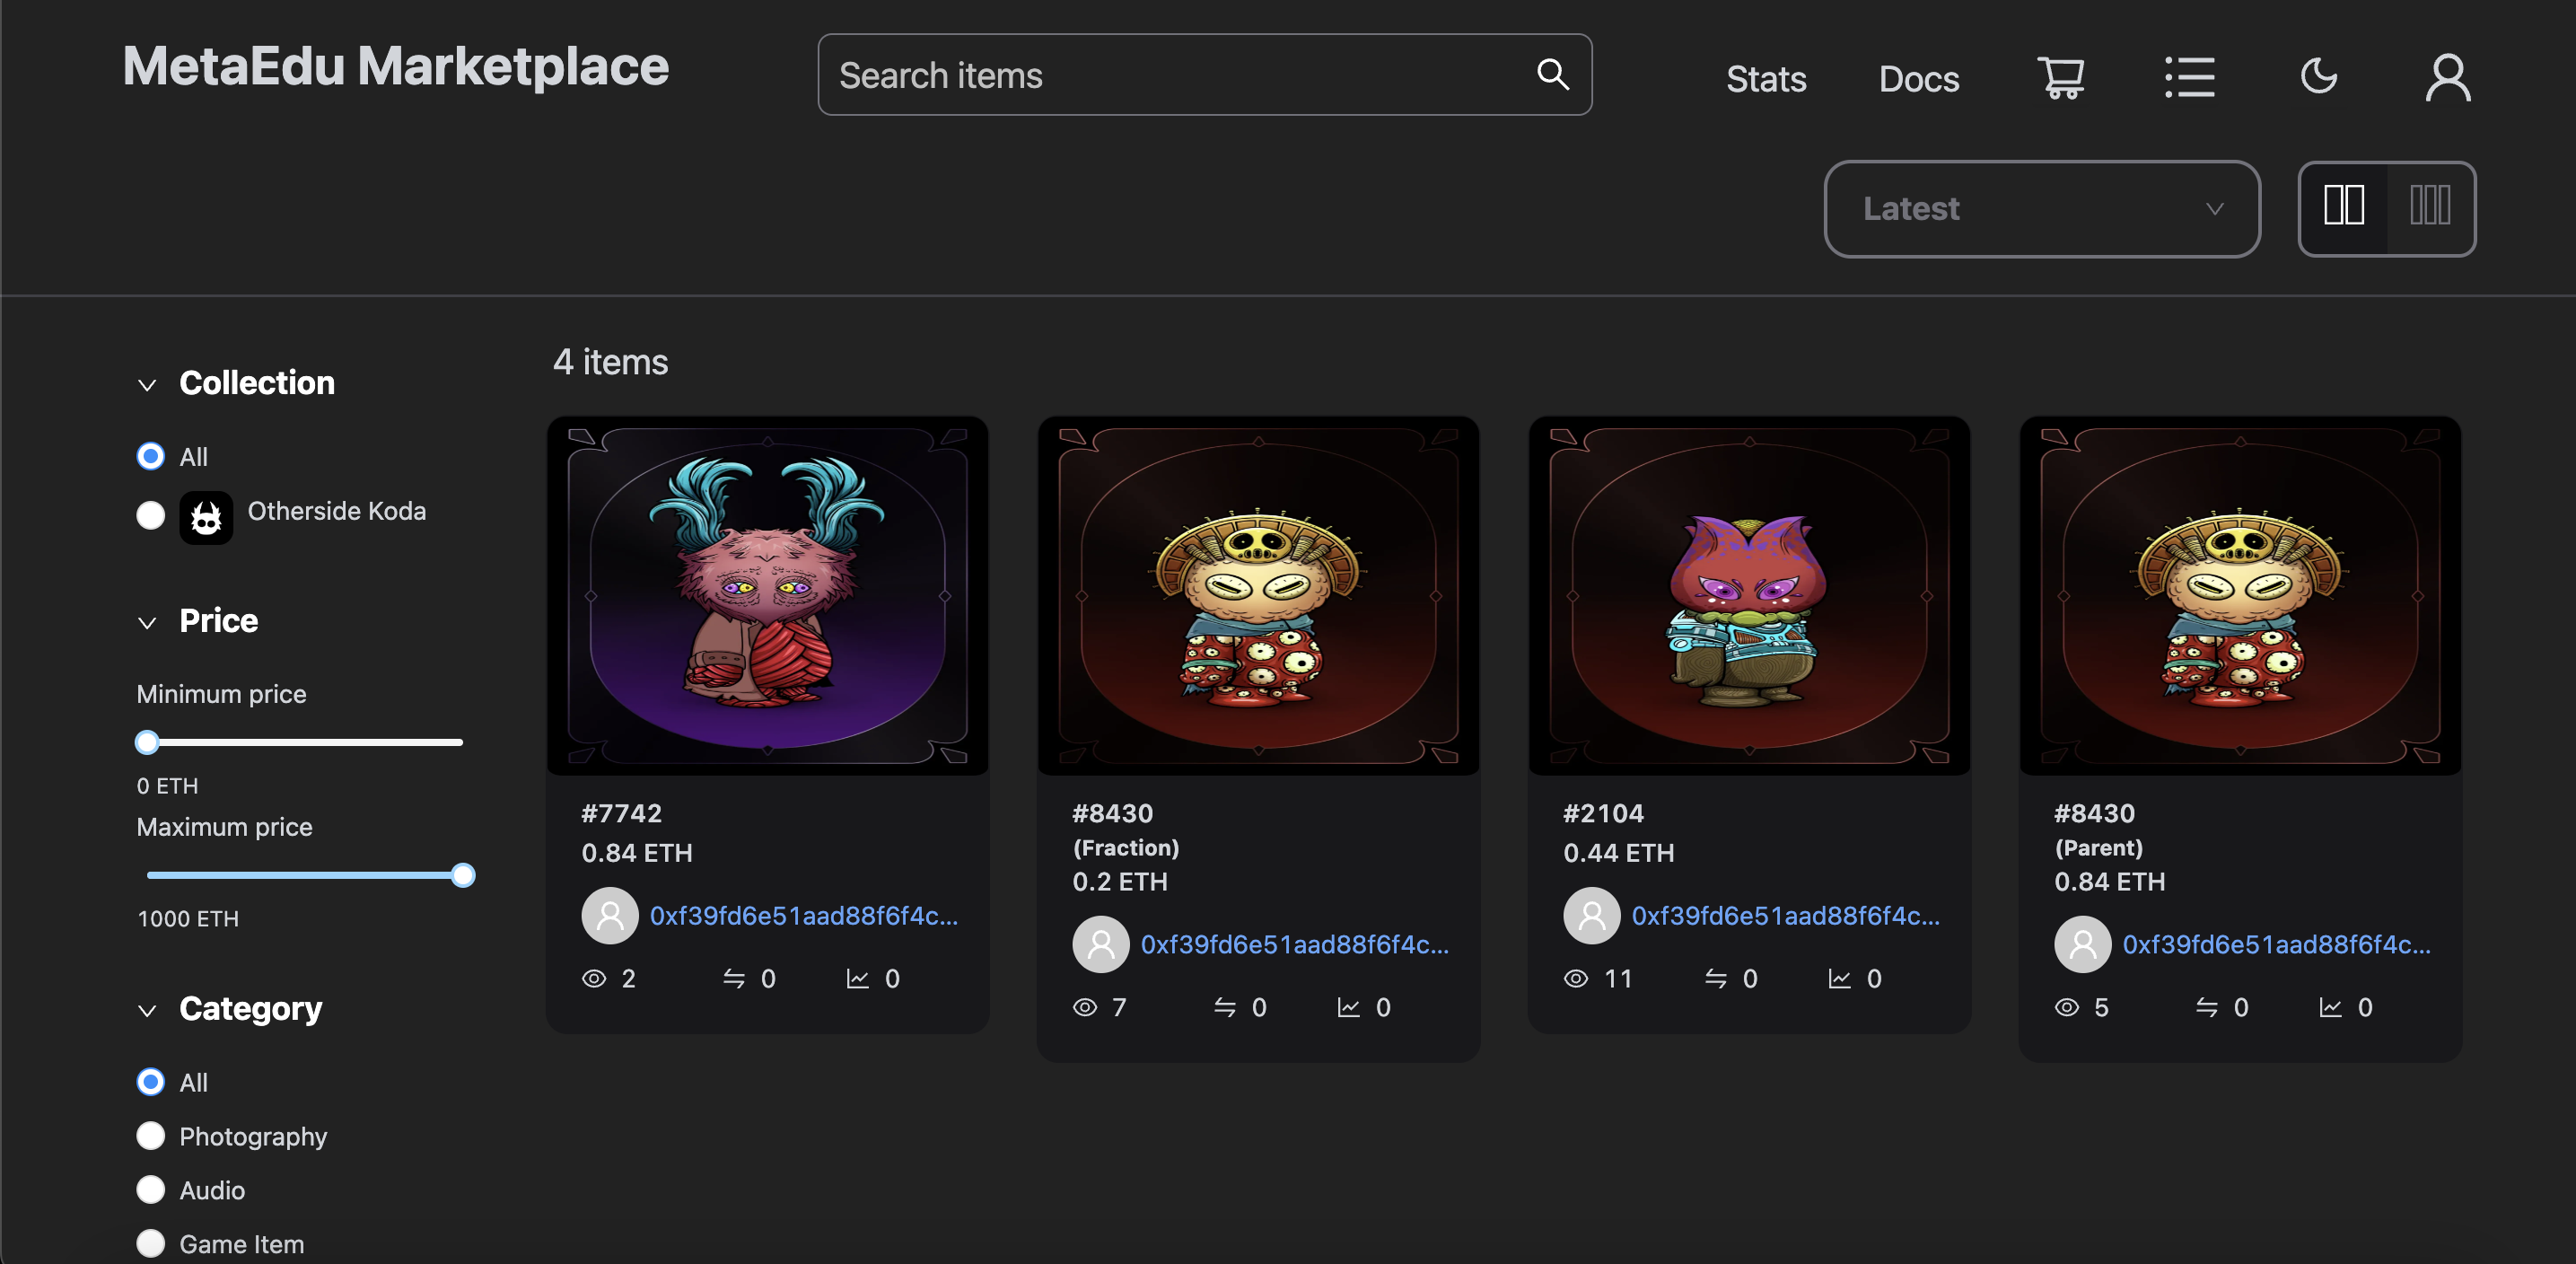
\includegraphics[scale=0.3]{gambar/img-frontend-search.png}
  \caption{Halaman pencarian \emph{Token}}
  \label{fig:TokenSearch}
\end{figure}

Halaman pencarian \emph{token} digunakan oleh \emph{user} untuk mencari \emph{token} tertentu berdasarkan nama, kategori, harga, dan koleksi.

\subsection{Halaman Detail Koleksi}
\begin{figure} [H] \centering
  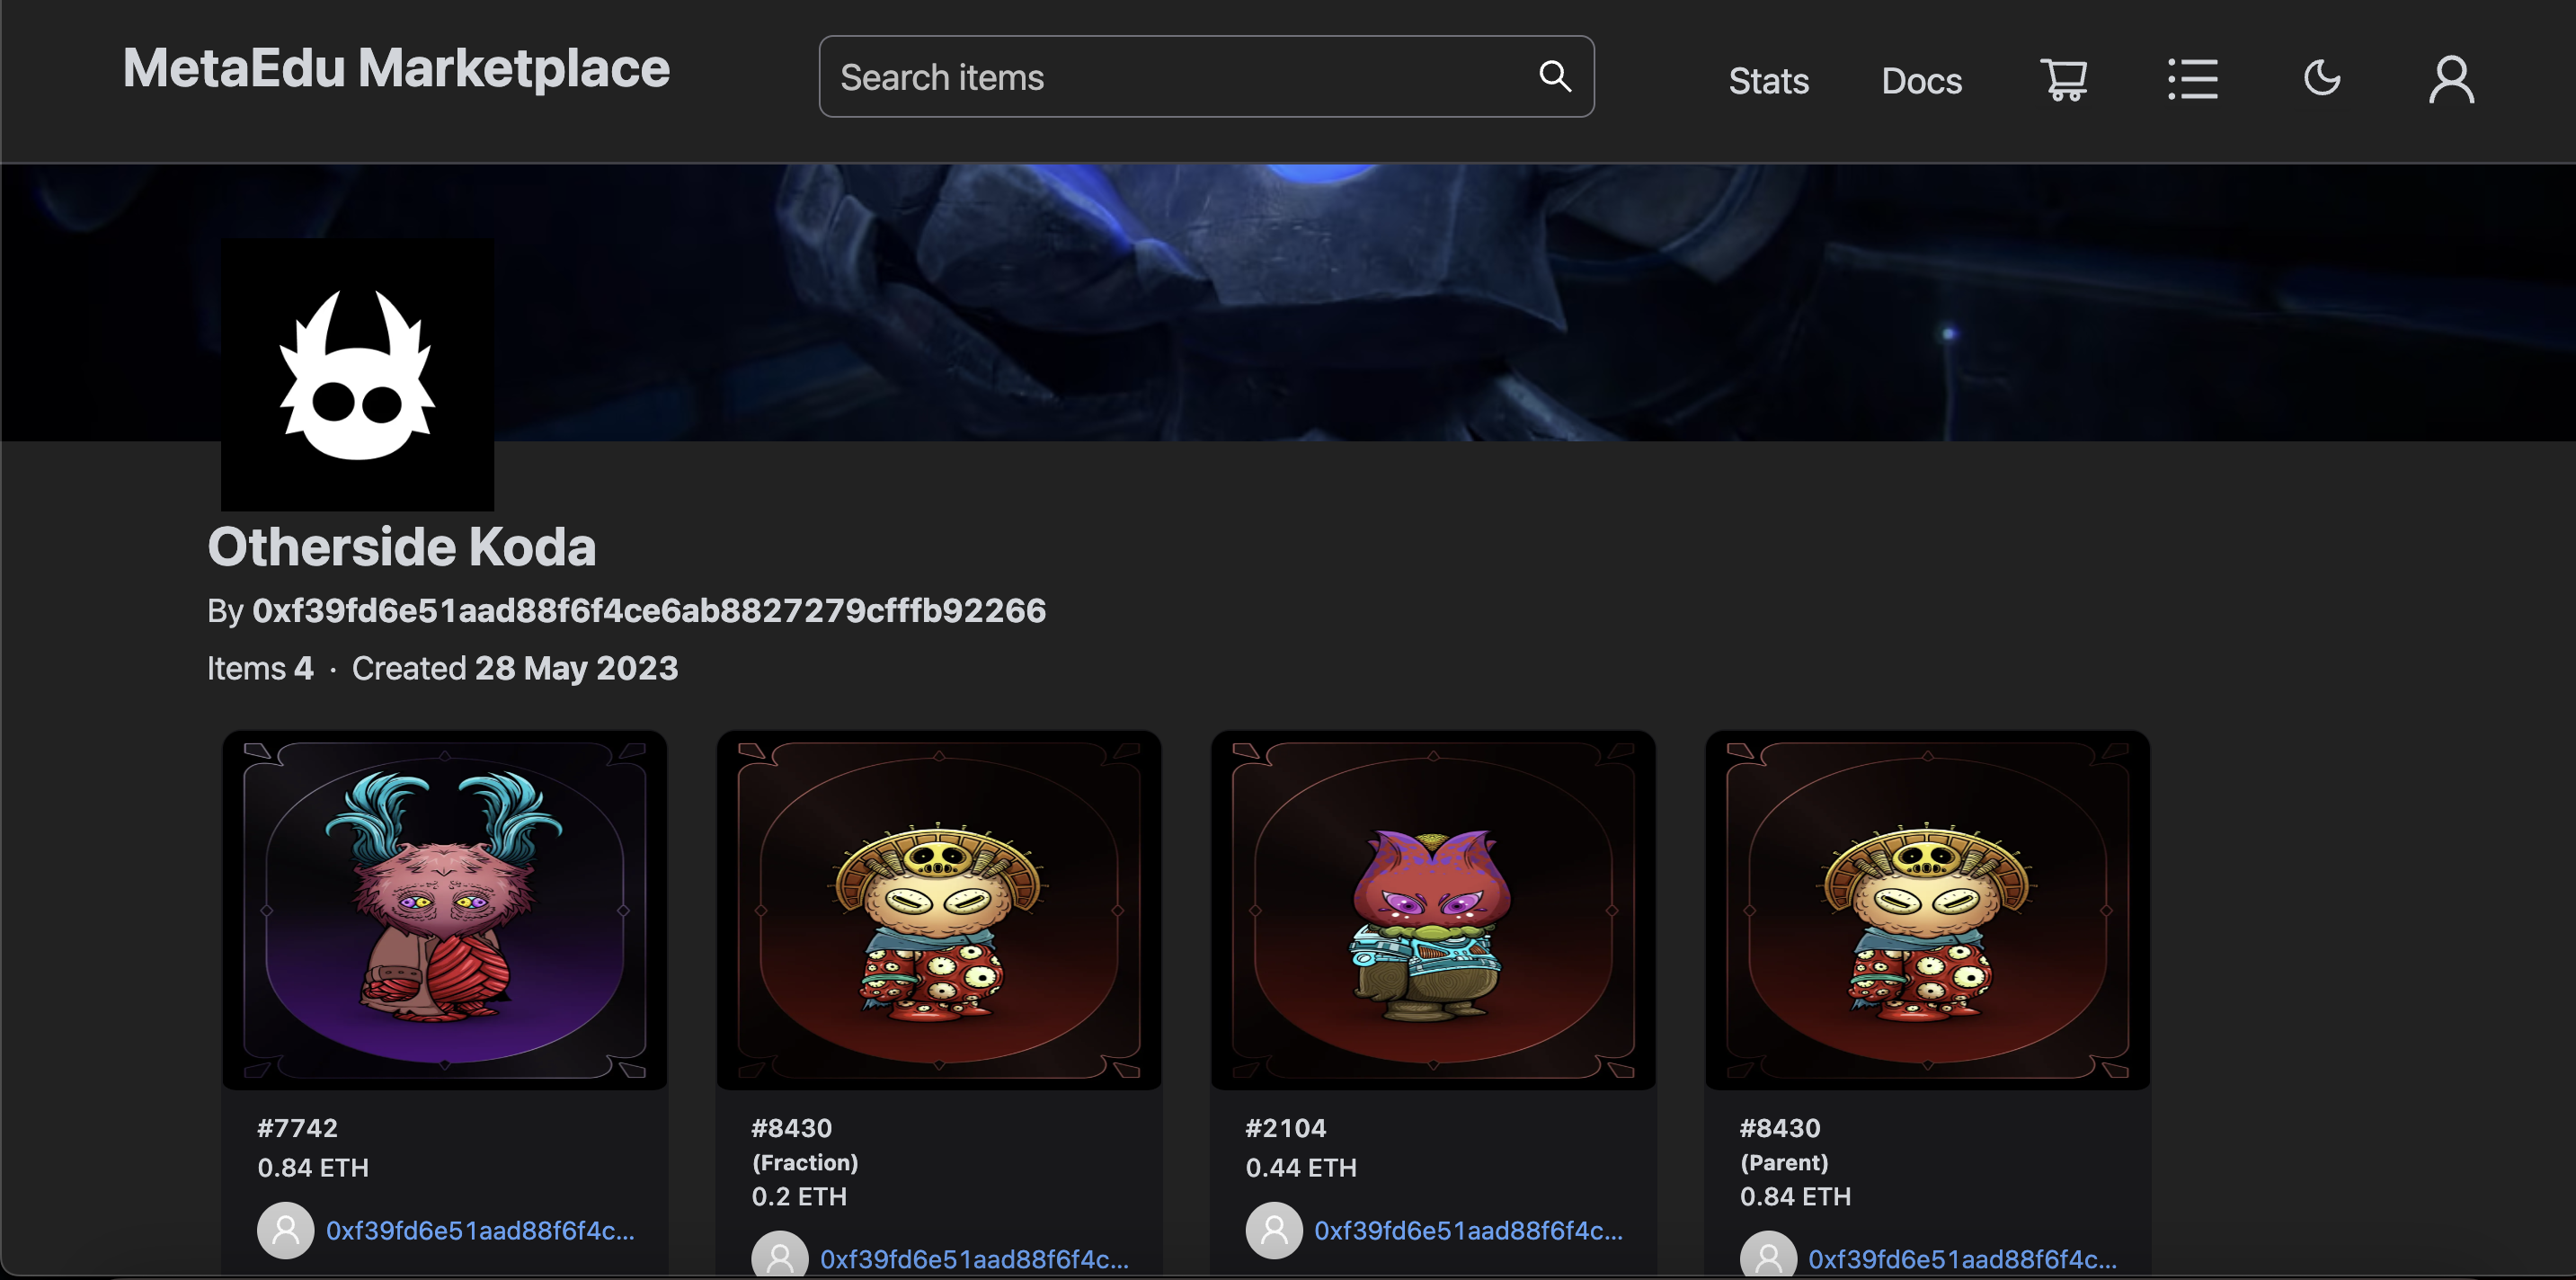
\includegraphics[scale=0.3]{gambar/img-frontend-collection.png}
  \caption{Halaman detail koleksi}
  \label{fig:CollectionDetail}
\end{figure}

Halaman detail koleksi berisi daftar token yang terkait dengan kolesi tersebut.

\subsection{Halaman Statistik}
\begin{figure} [H] \centering
  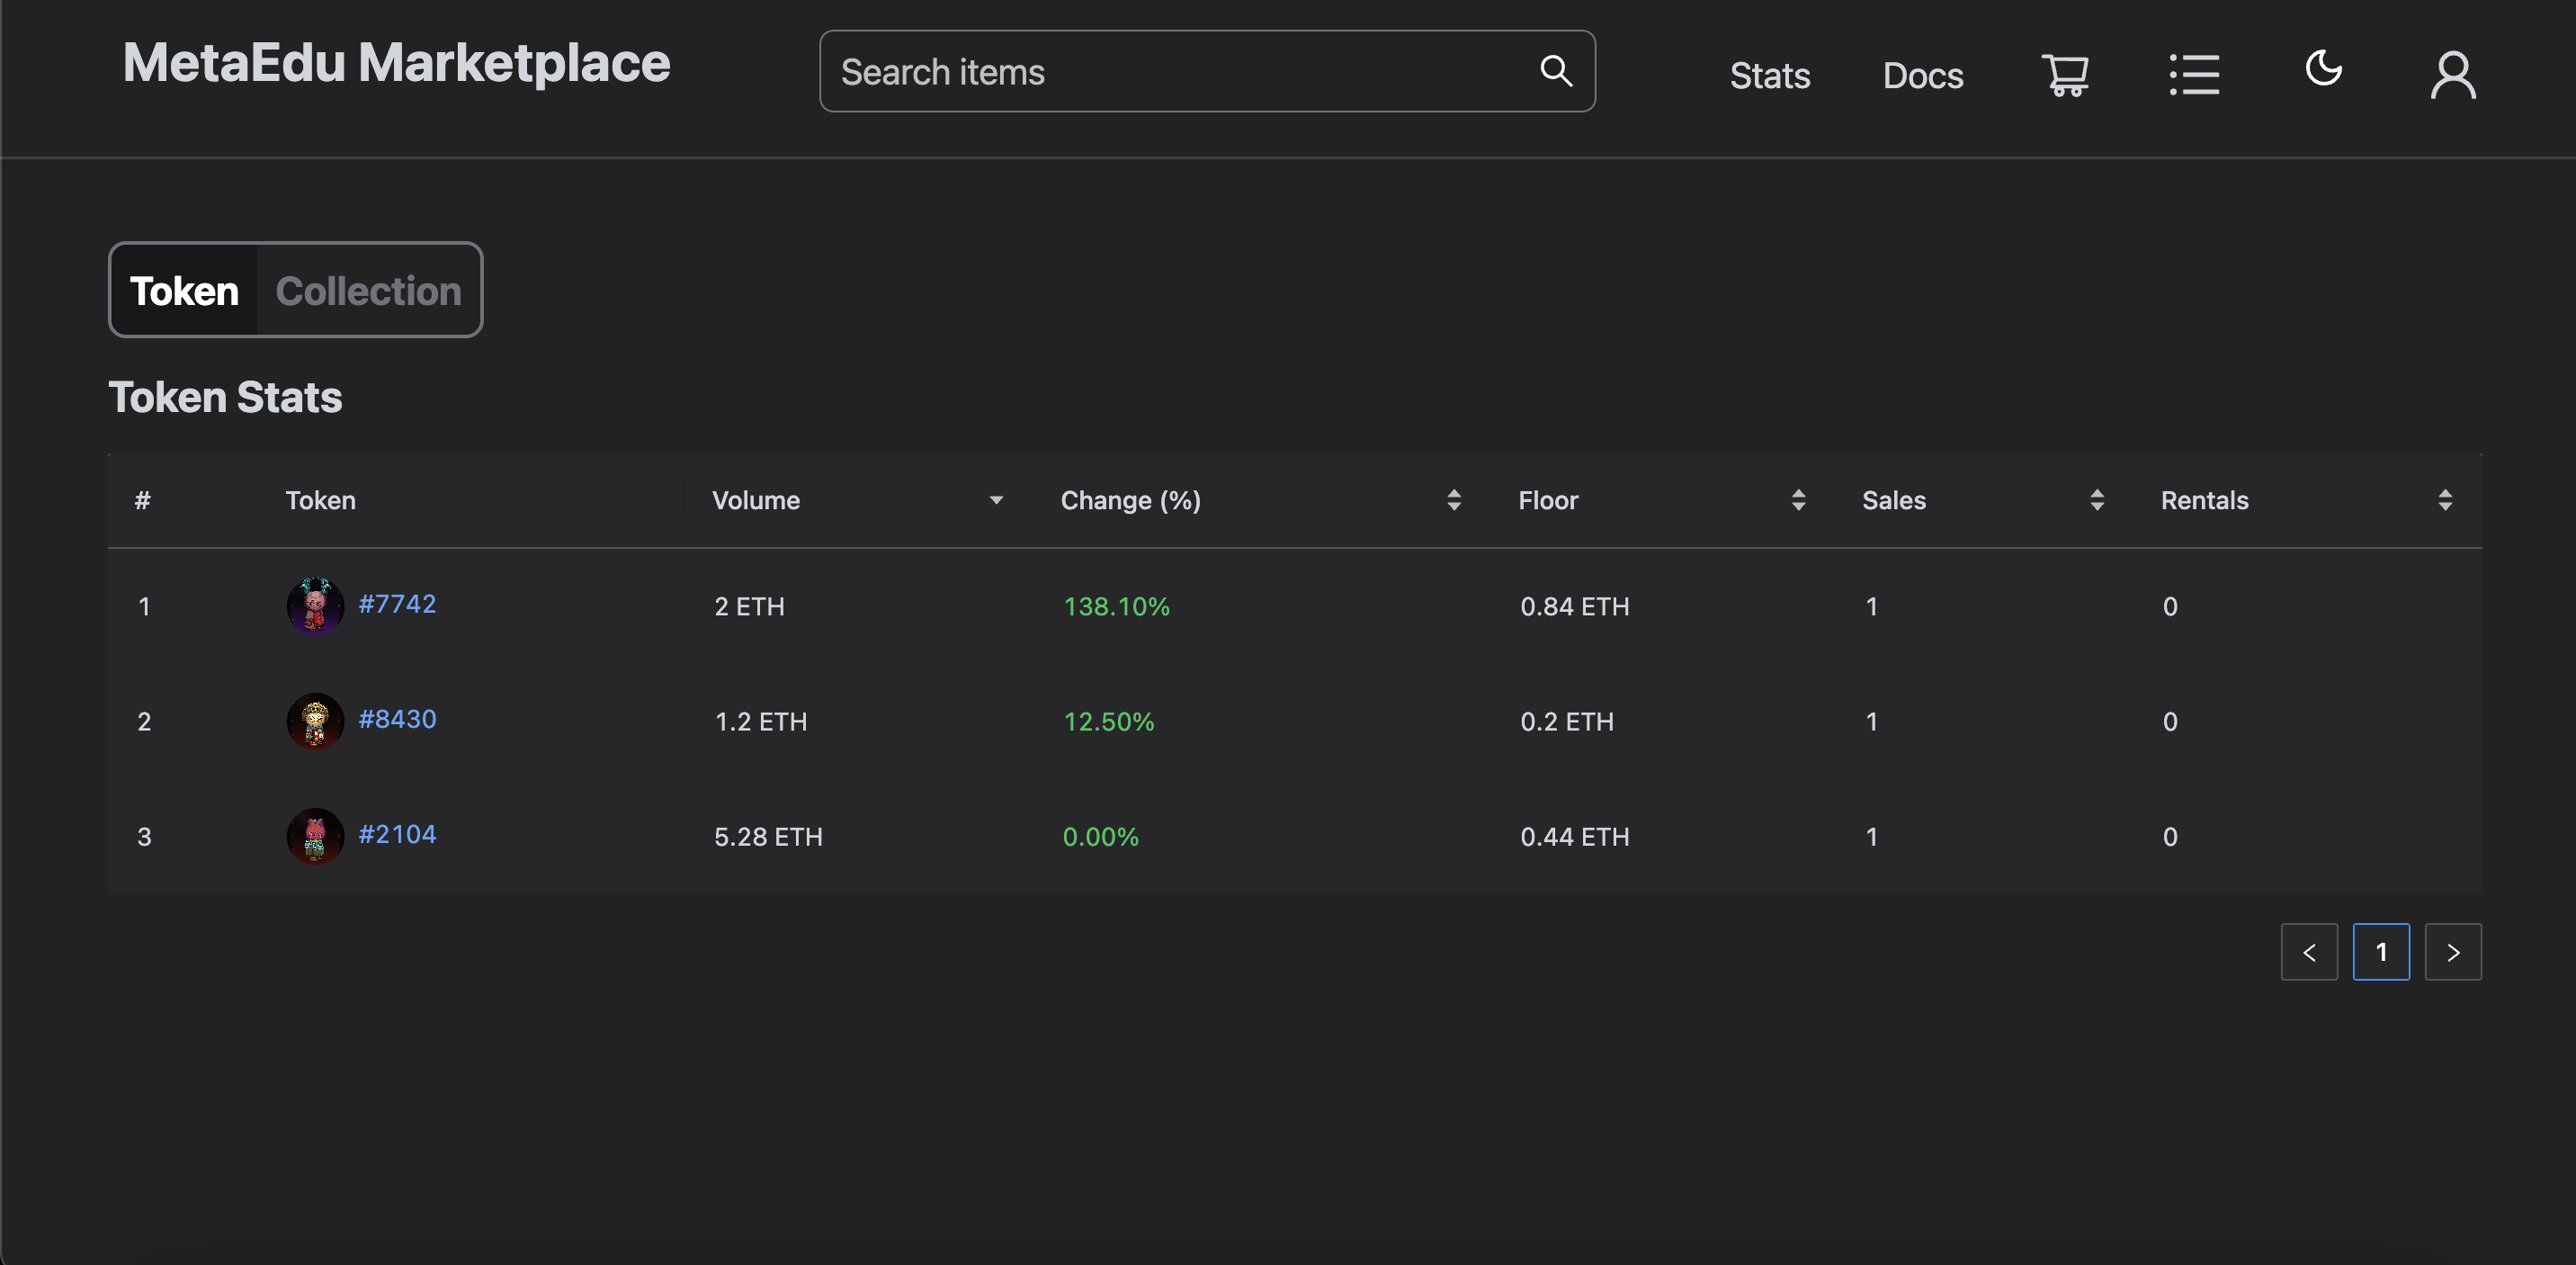
\includegraphics[scale=0.3]{gambar/img-frontend-stats.png}
  \caption{Halaman statistik}
  \label{fig:TokenStats}
\end{figure}

Halaman statistik berisi daftar token dan koleksi yang diurutkan berdasarkan parameter seperti \emph{Volume}, perubahan harga, \emph{floor} / harga terbawah, jumlah penjualan dan jumlah penyewaan.

\subsection{Halaman Dokumentasi}
\begin{figure} [H] \centering
  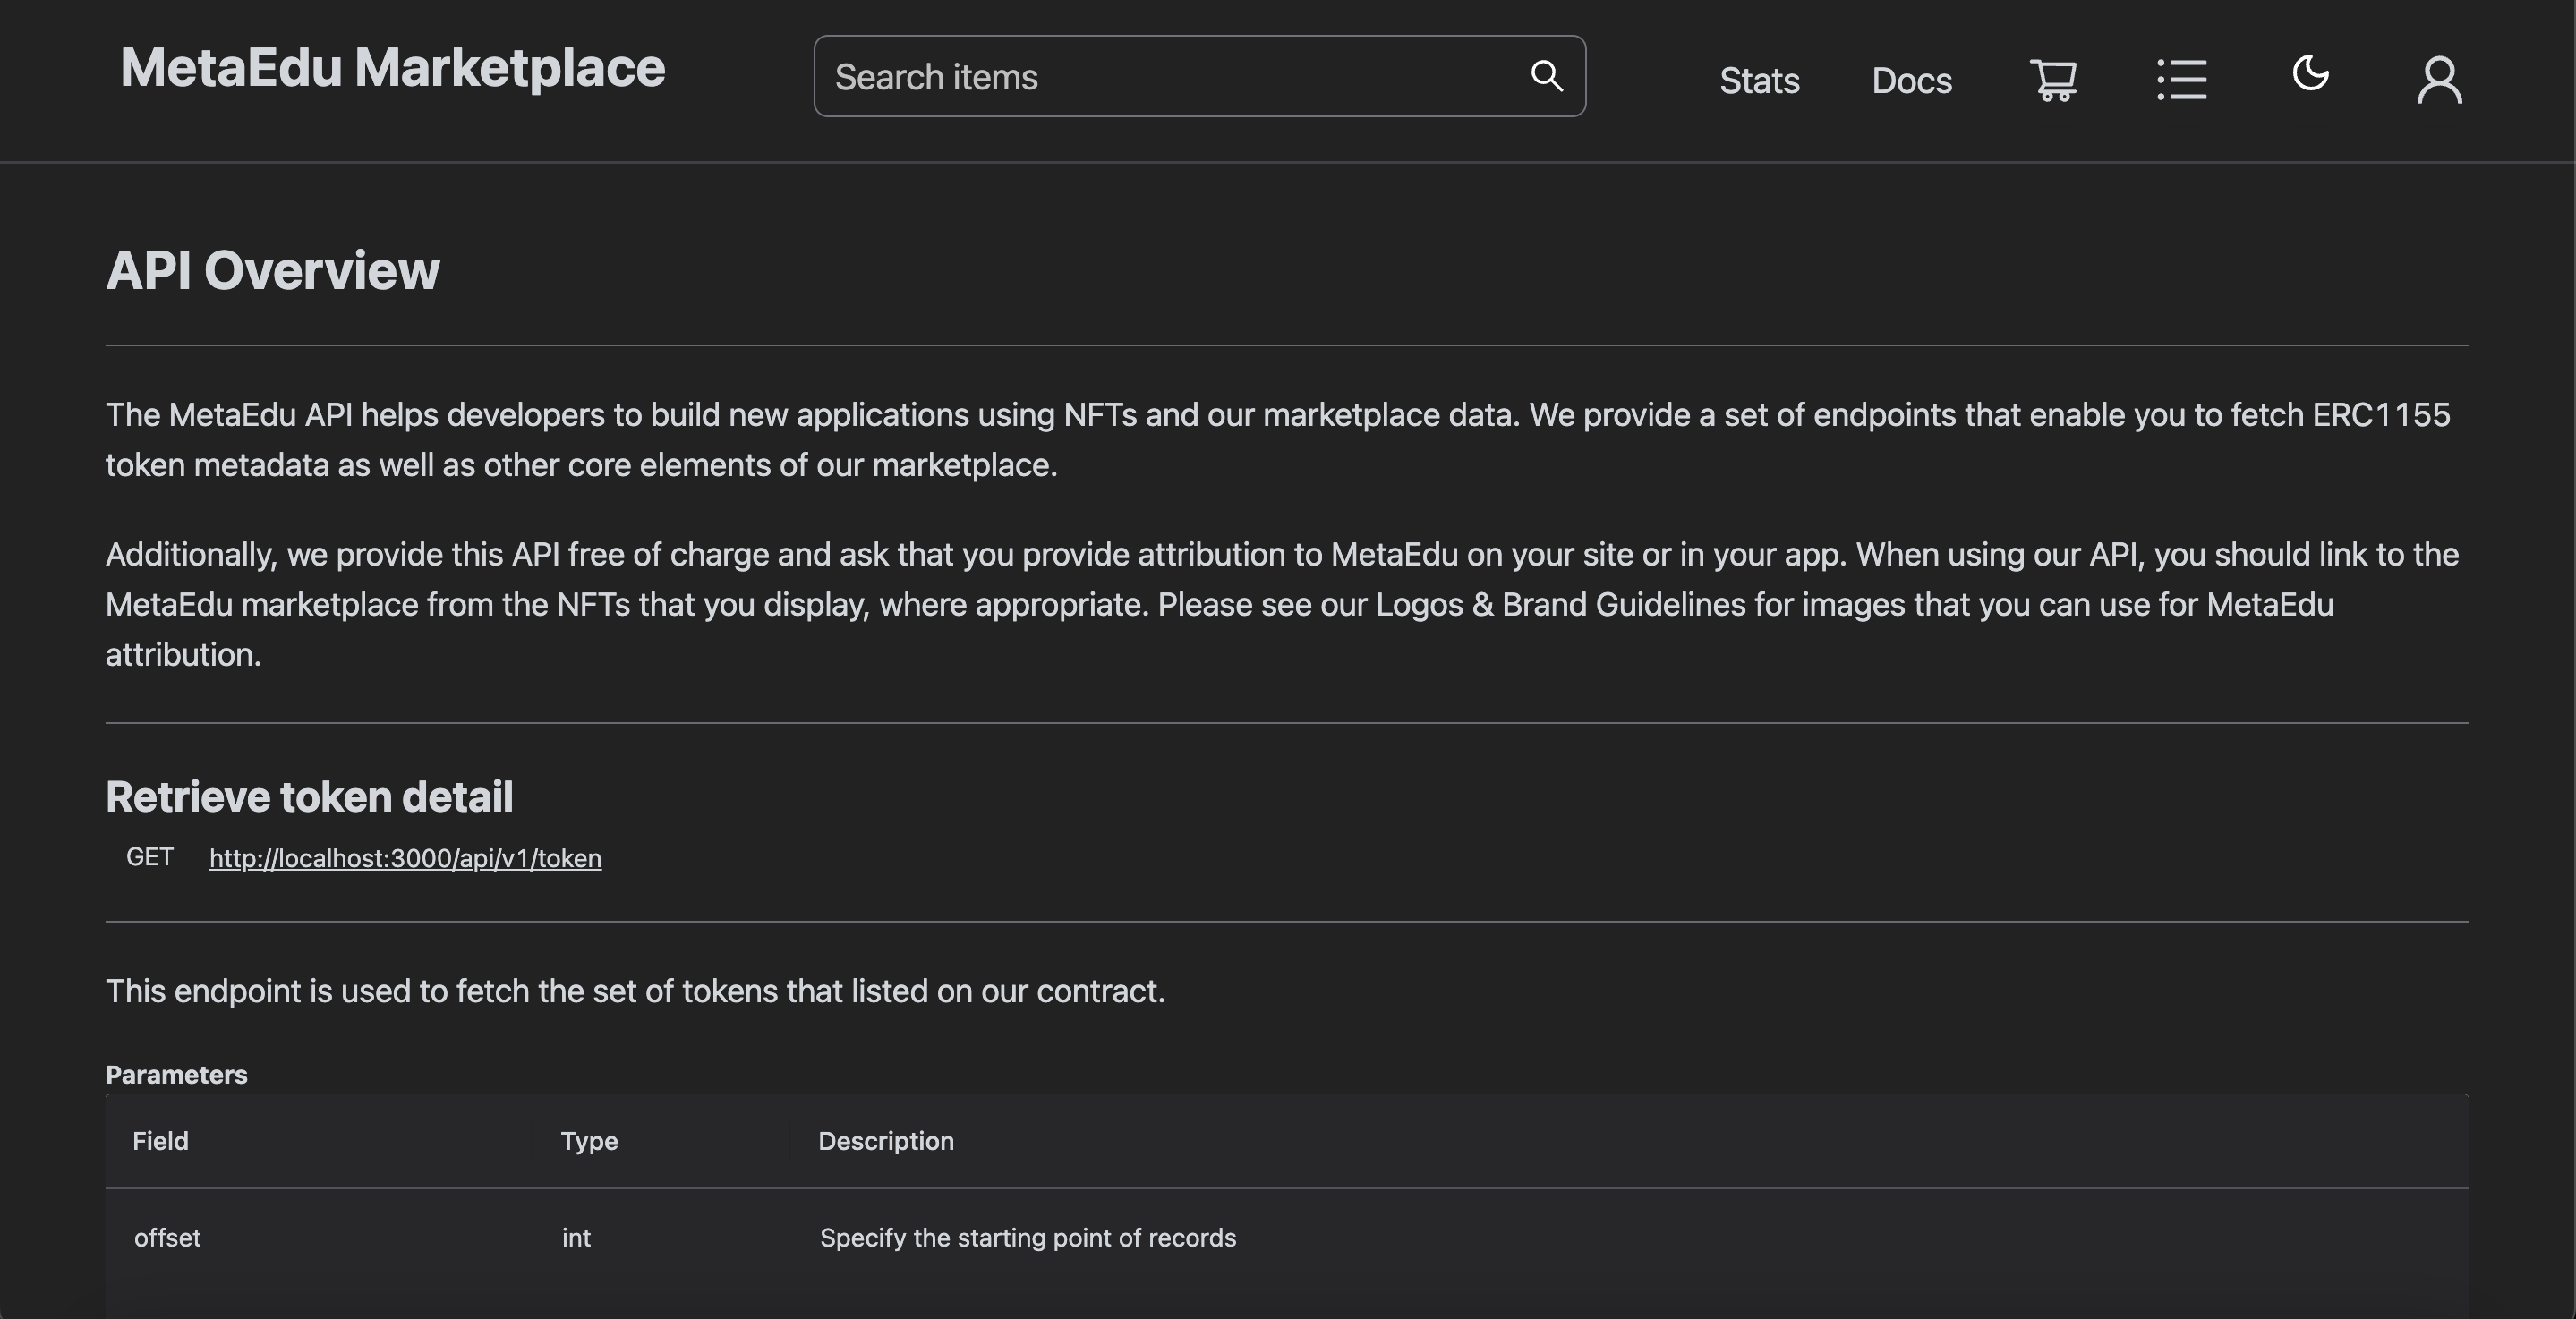
\includegraphics[scale=0.3]{gambar/img-frontend-api.png}
  \caption{Halaman dokumentasi}
  \label{fig:Docs}
\end{figure}

Halaman dokumentasi berisi informasi mengenai \emph{API} yang disedikan untuk \emph{platform} lain dapat memanfaatkan data dari \emph{NFT Marketplace} ini seperti data token, kepemilikan, dan penyewaan.

\section{Pengembangan \emph{Metaverse}} 

\emph{Metaverse} yang dikembangkan digunakan untuk menguji apakah API yang telah dikembangkan dapat diintegrasikan ke dalam \emph{metaverse} tersebut. Software yang digunakan untuk mengembangkan \emph{metaverse} ini adalah Unity. Untuk melakukan proses autentikasi mengunakan \emph{metamask} digunakan \emph{library} \emph{Web3Unity}. 

\subsection{Halaman Autentikas} 

\begin{figure} [H] \centering
  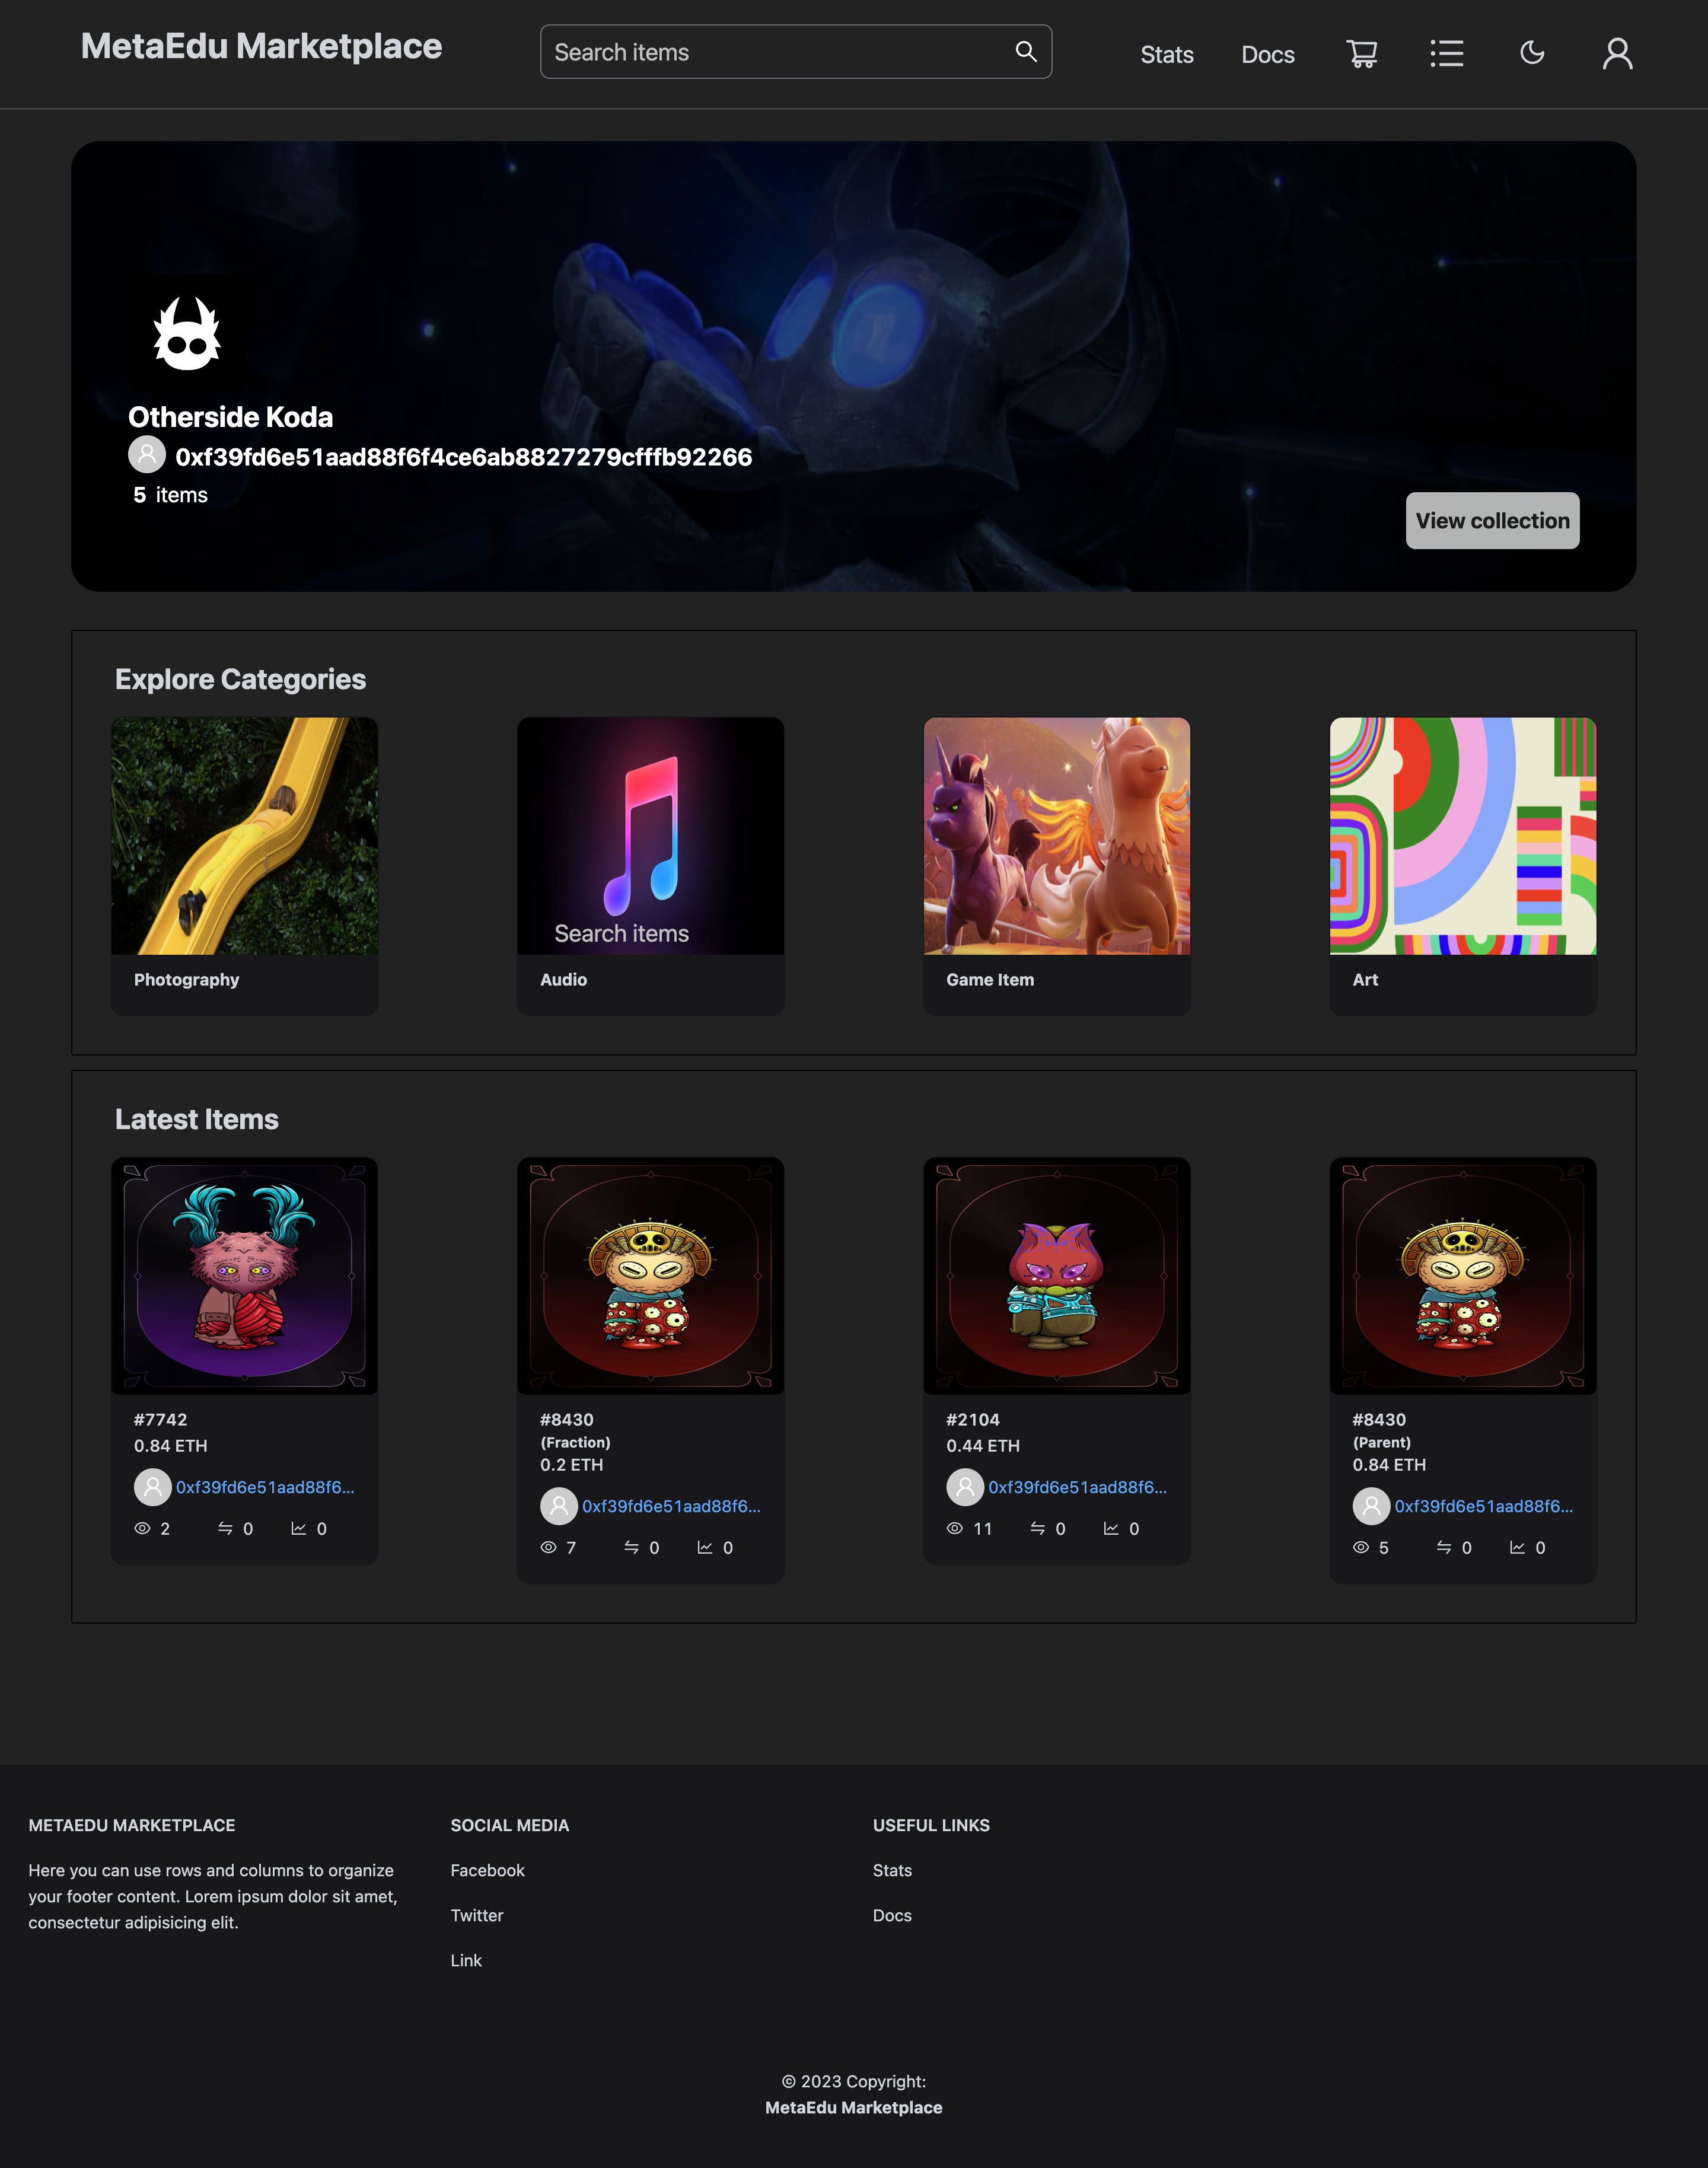
\includegraphics[scale=0.12]{gambar/img-frontend-index.png}
  \caption{Halaman awal \emph{NFT Marketplace}}
  \label{fig:NFTMarketplace}
\end{figure}

Tampilan awal \emph{NFT Marketplace}, menampilkan koleksi \emph{token}, kategori \emph{token}, dan \emph{token} terbaru.

\begin{figure} [H] \centering
  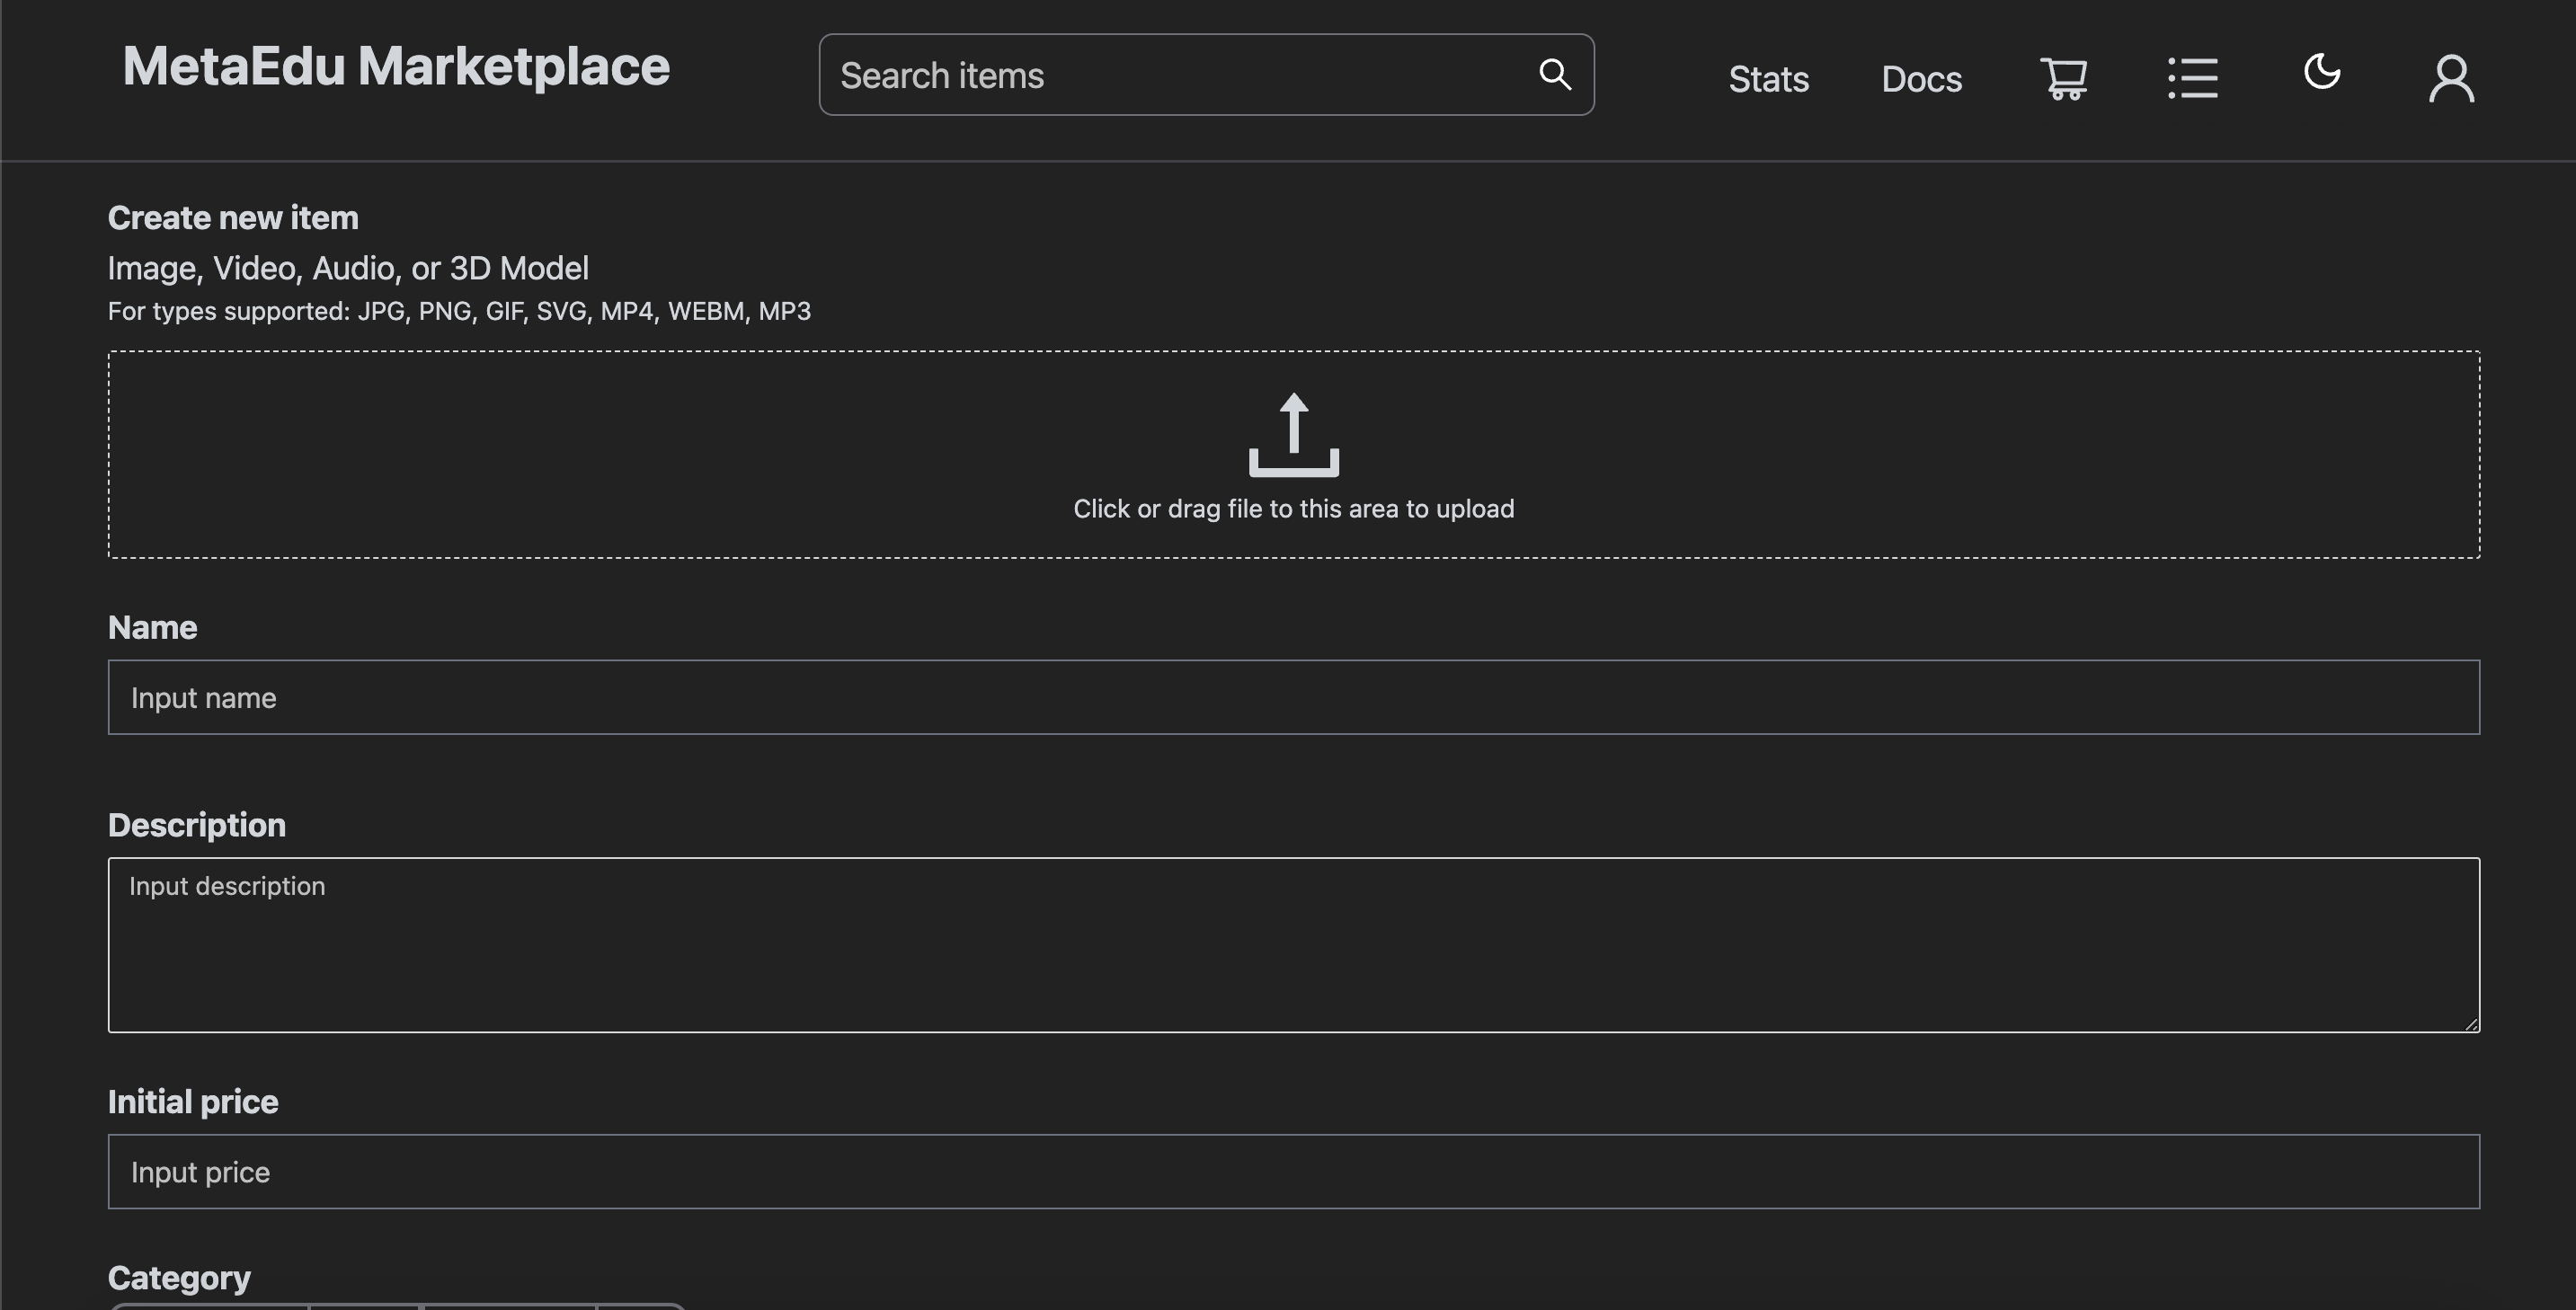
\includegraphics[scale=0.3]{gambar/img-frontend-add-token.png}
  \caption{Halaman \emph{Minting Token}}
  \label{fig:TokenMinting}
\end{figure}

Halaman \emph{Minting token} merupakan halaman yang digunakan \emph{user} untuk membuat \emph{token} baru. Untuk membuat \emph{token} baru, \emph{user} perlu memasukan \emph{image} \emph{token}, nama \emph{token}, harga awal, suplai, dan koleksi. 

\subsection{Halaman Detail \emph{Token}}

\begin{figure} [H] \centering
  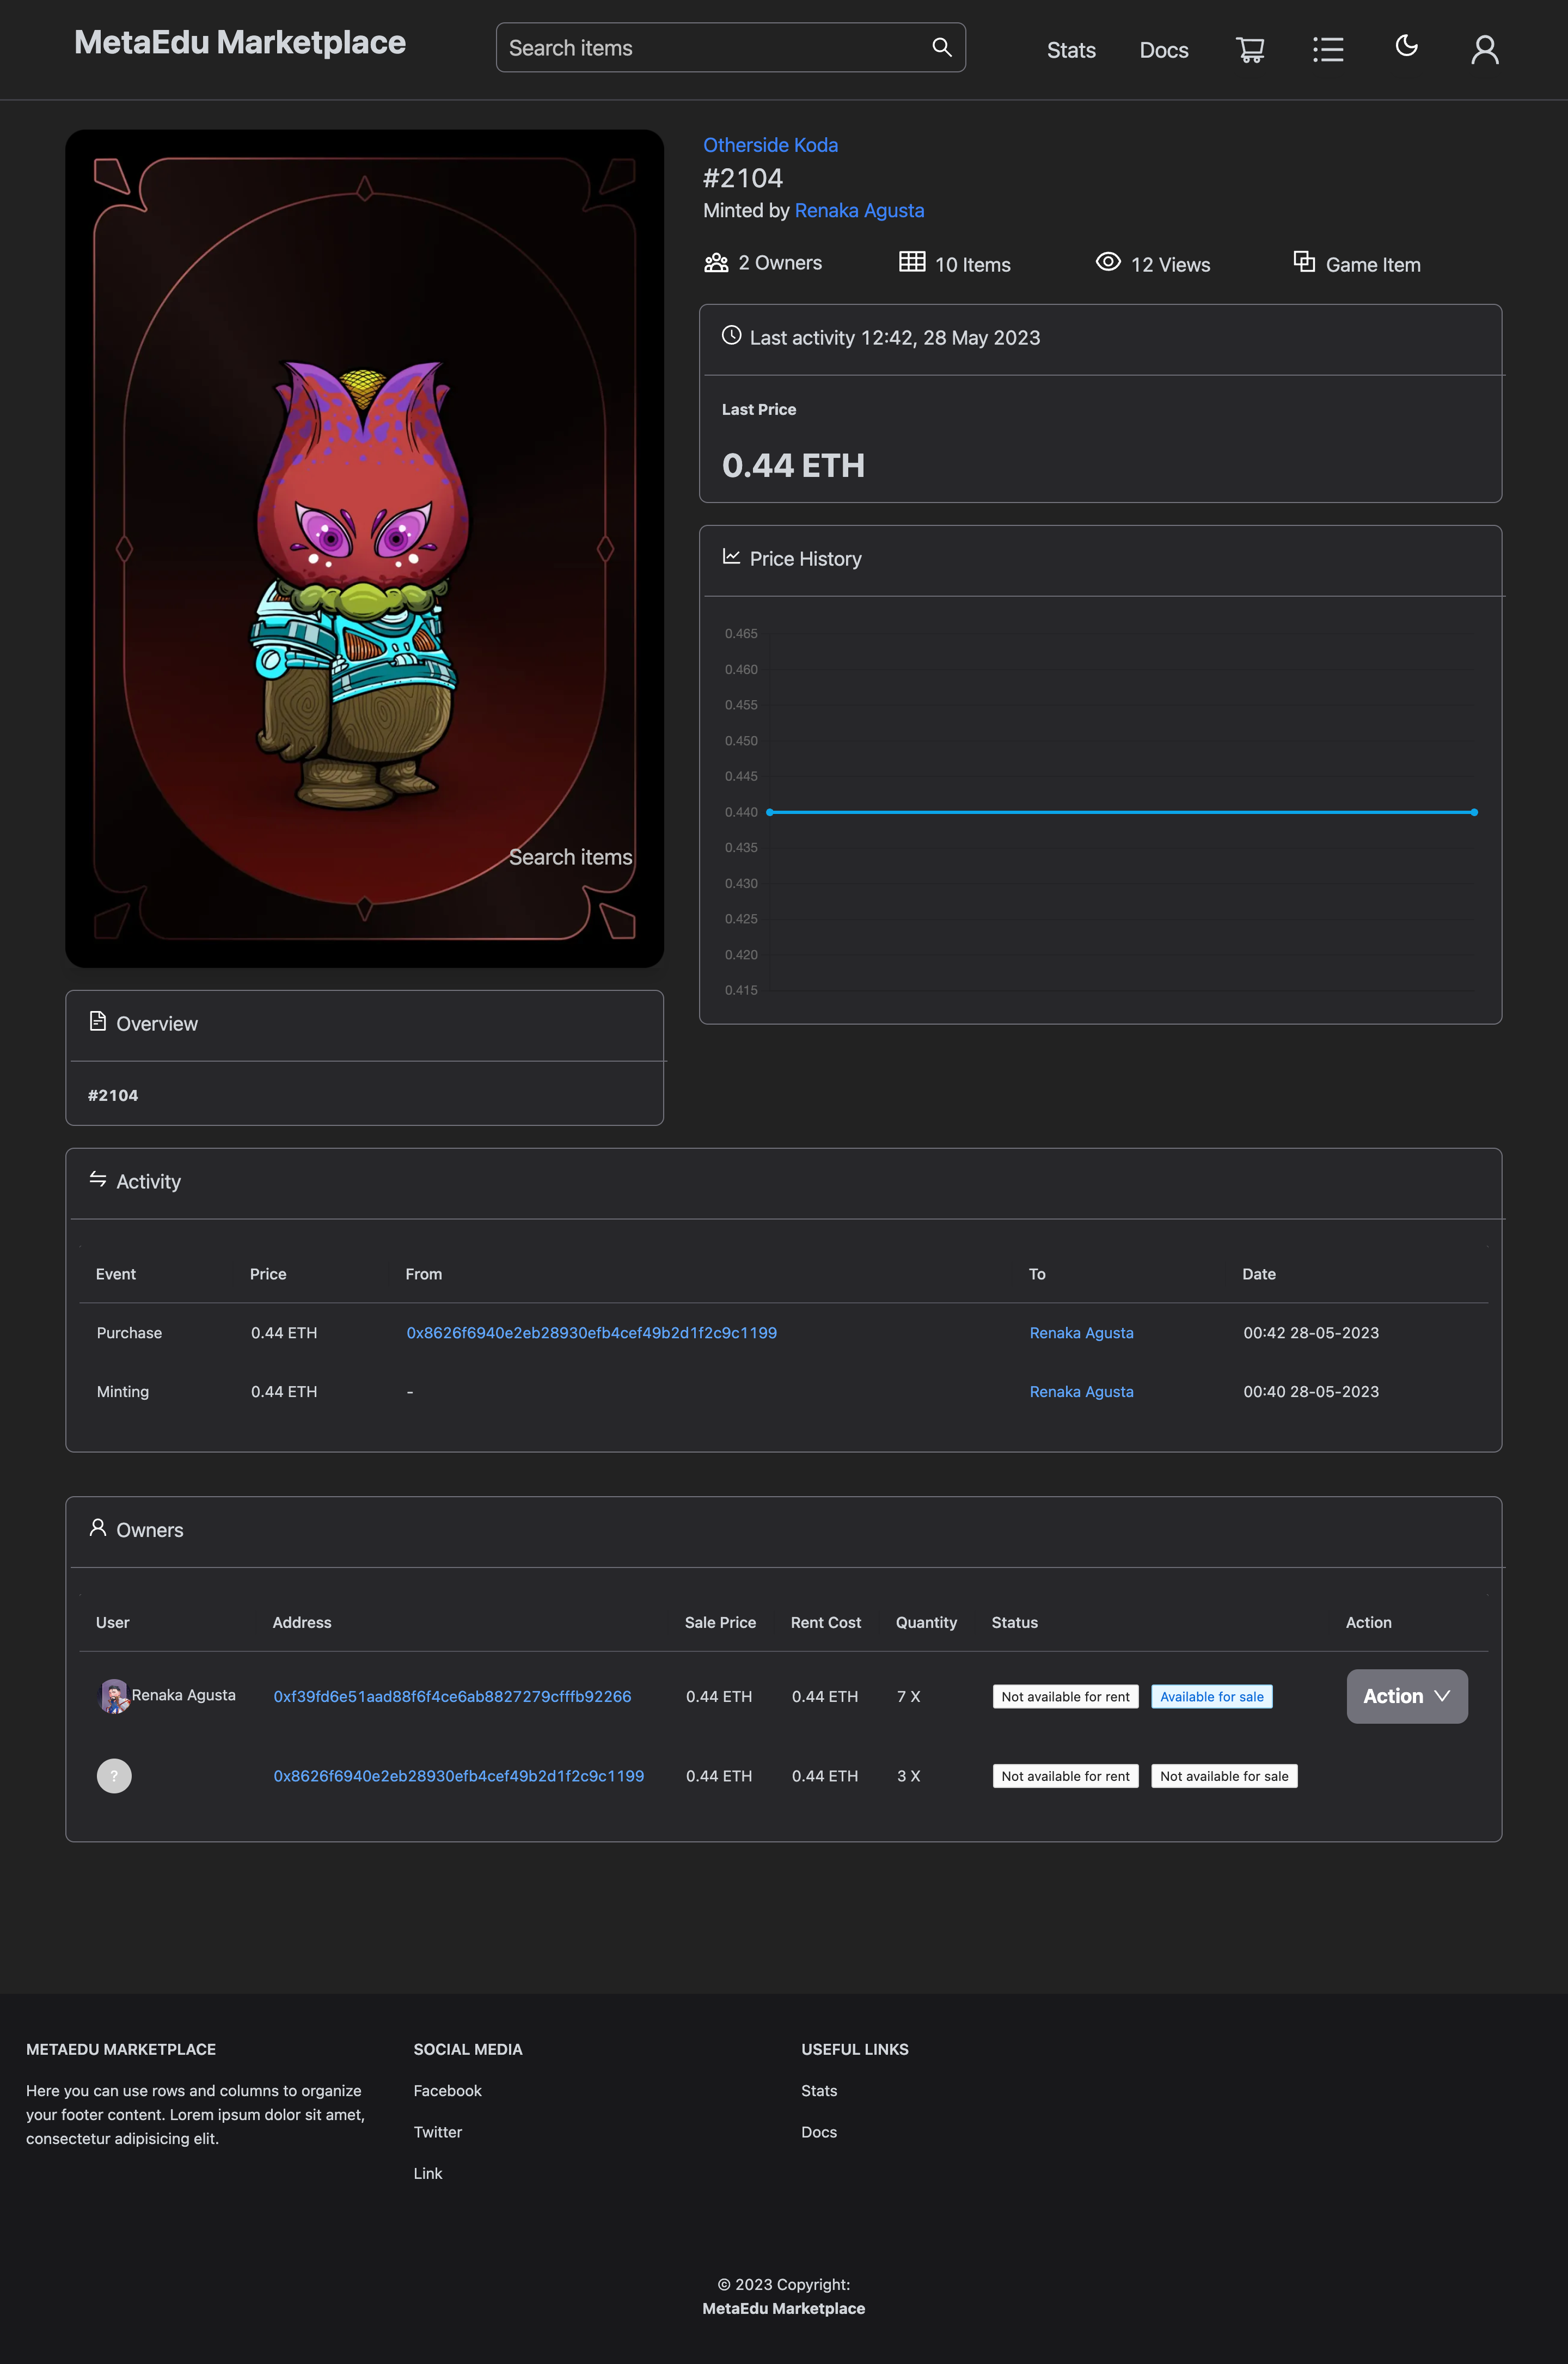
\includegraphics[scale=0.1]{gambar/img-frontend-token-detail.png}
  \caption{Halaman detail \emph{Token}}
  \label{fig:TokenDetail}
\end{figure}

Halaman detail \emph{token} menampilkan informasi-informasi mengenai nama \emph{token}, harga terakhir, pergerakan harga, riwayat transaksi, daftar kepemilkan dan lainnya. 

\subsection{Halaman Pencarian \emph{Token}}
\begin{figure} [H] \centering
  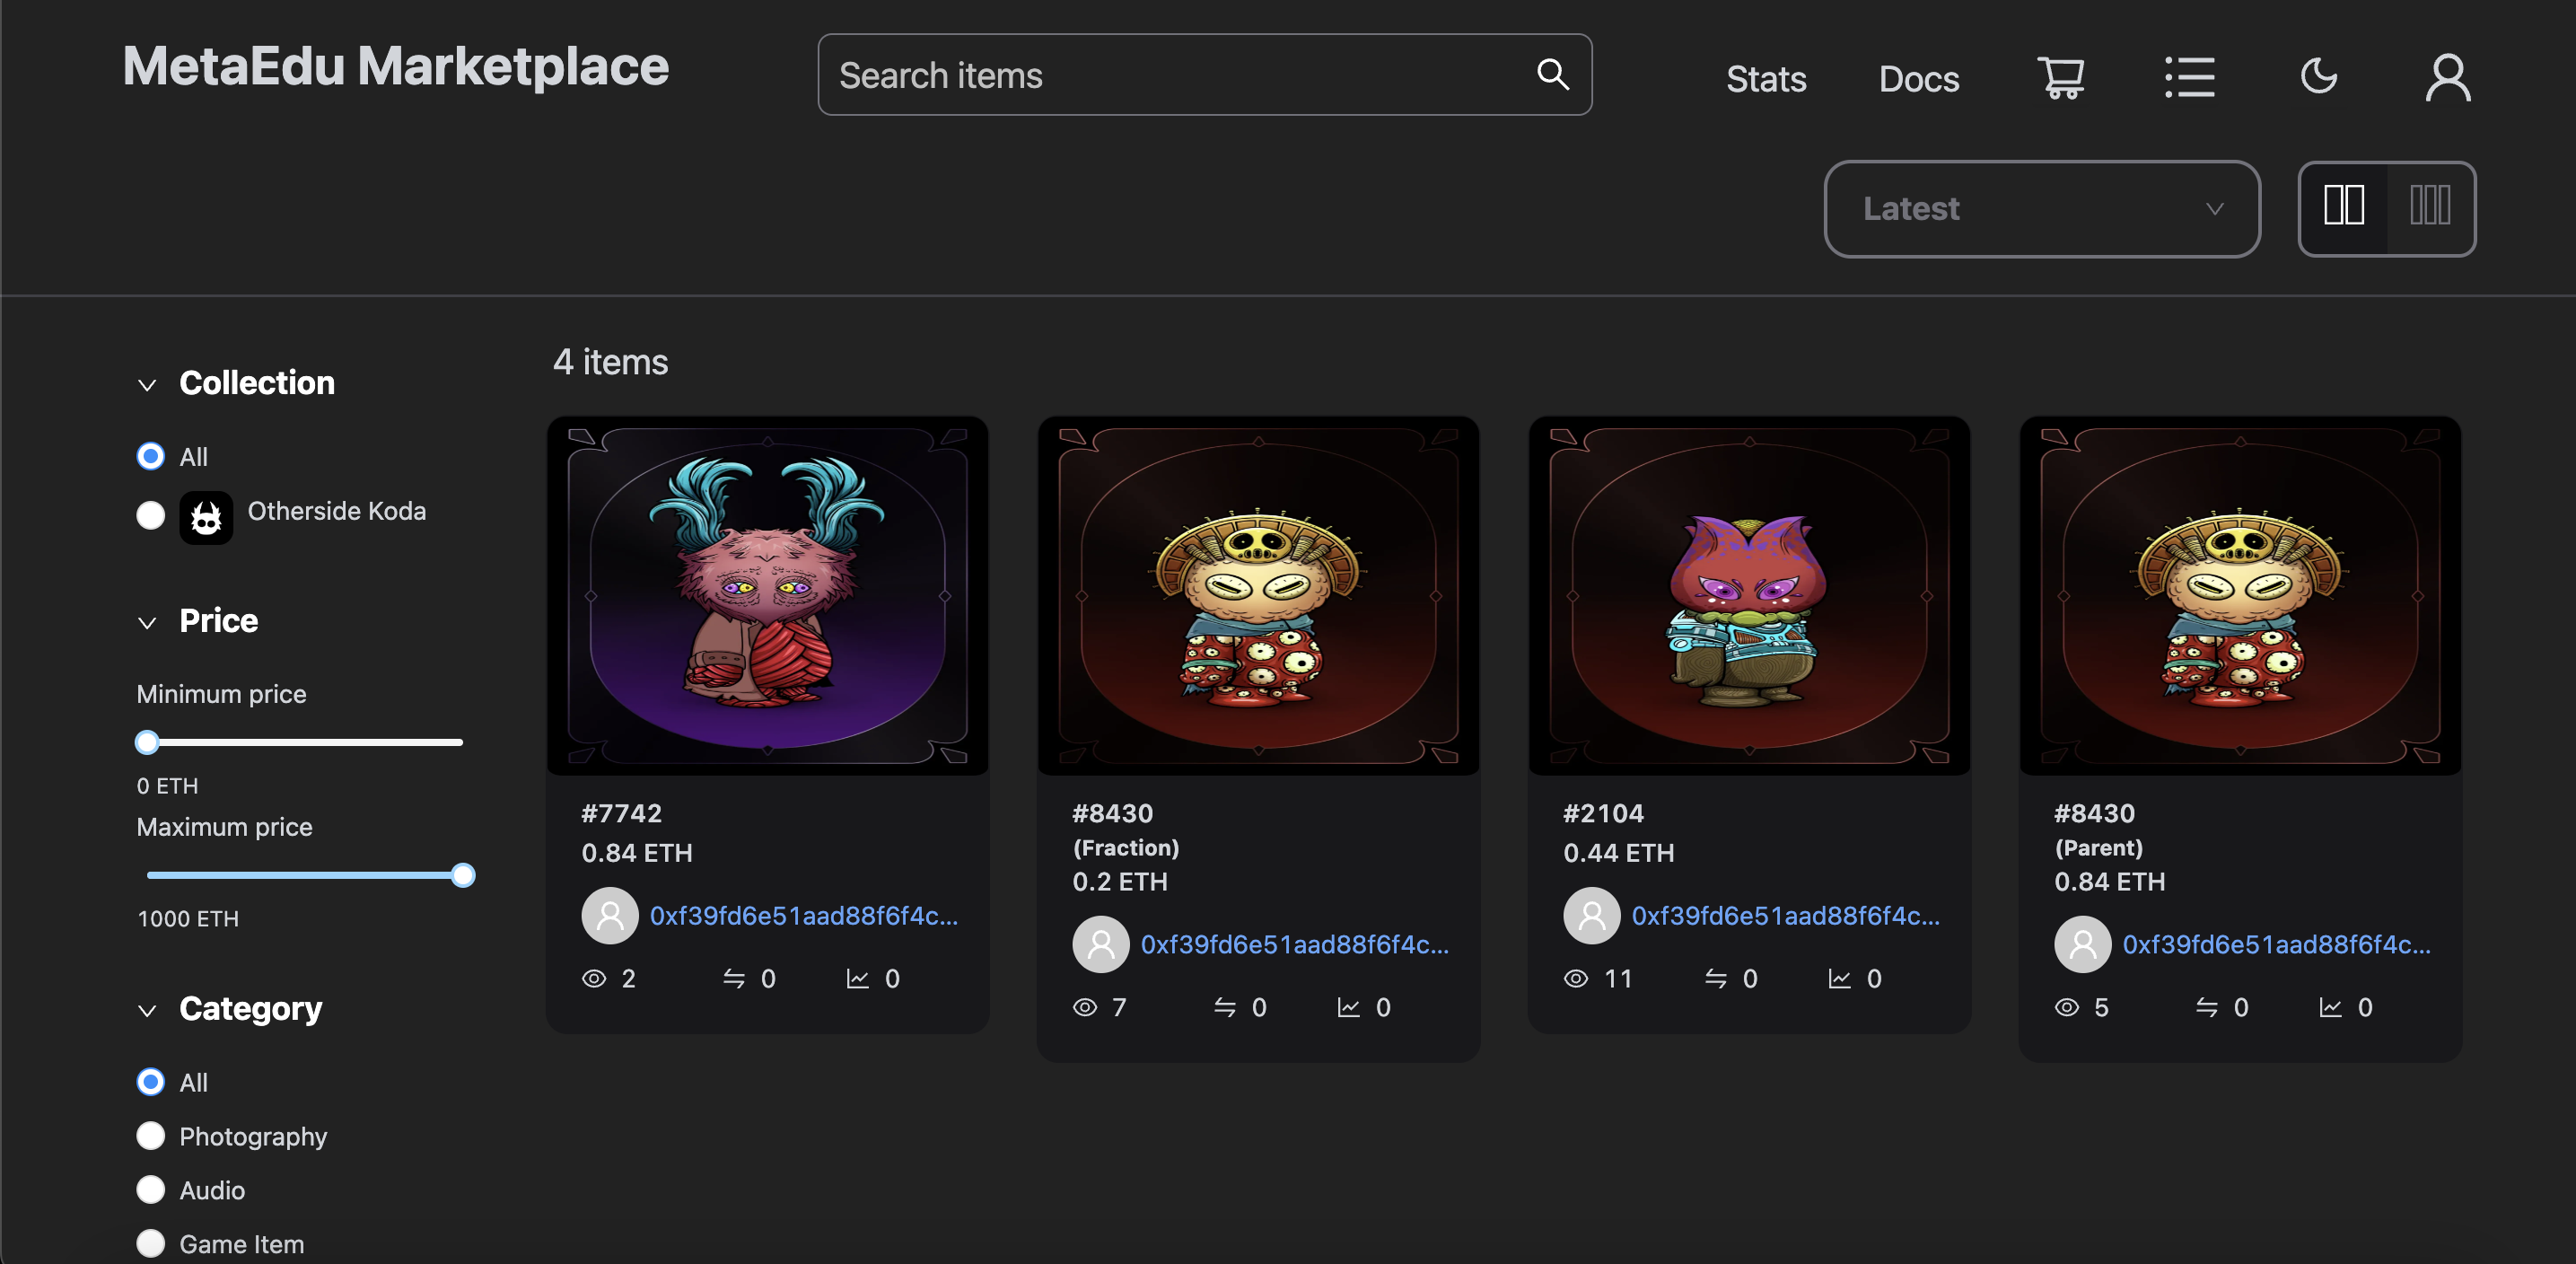
\includegraphics[scale=0.3]{gambar/img-frontend-search.png}
  \caption{Halaman pencarian \emph{Token}}
  \label{fig:TokenSearch}
\end{figure}

Halaman pencarian \emph{token} digunakan oleh \emph{user} untuk mencari \emph{token} tertentu berdasarkan nama, kategori, harga, dan koleksi.

\subsection{Halaman Detail Koleksi}
\begin{figure} [H] \centering
  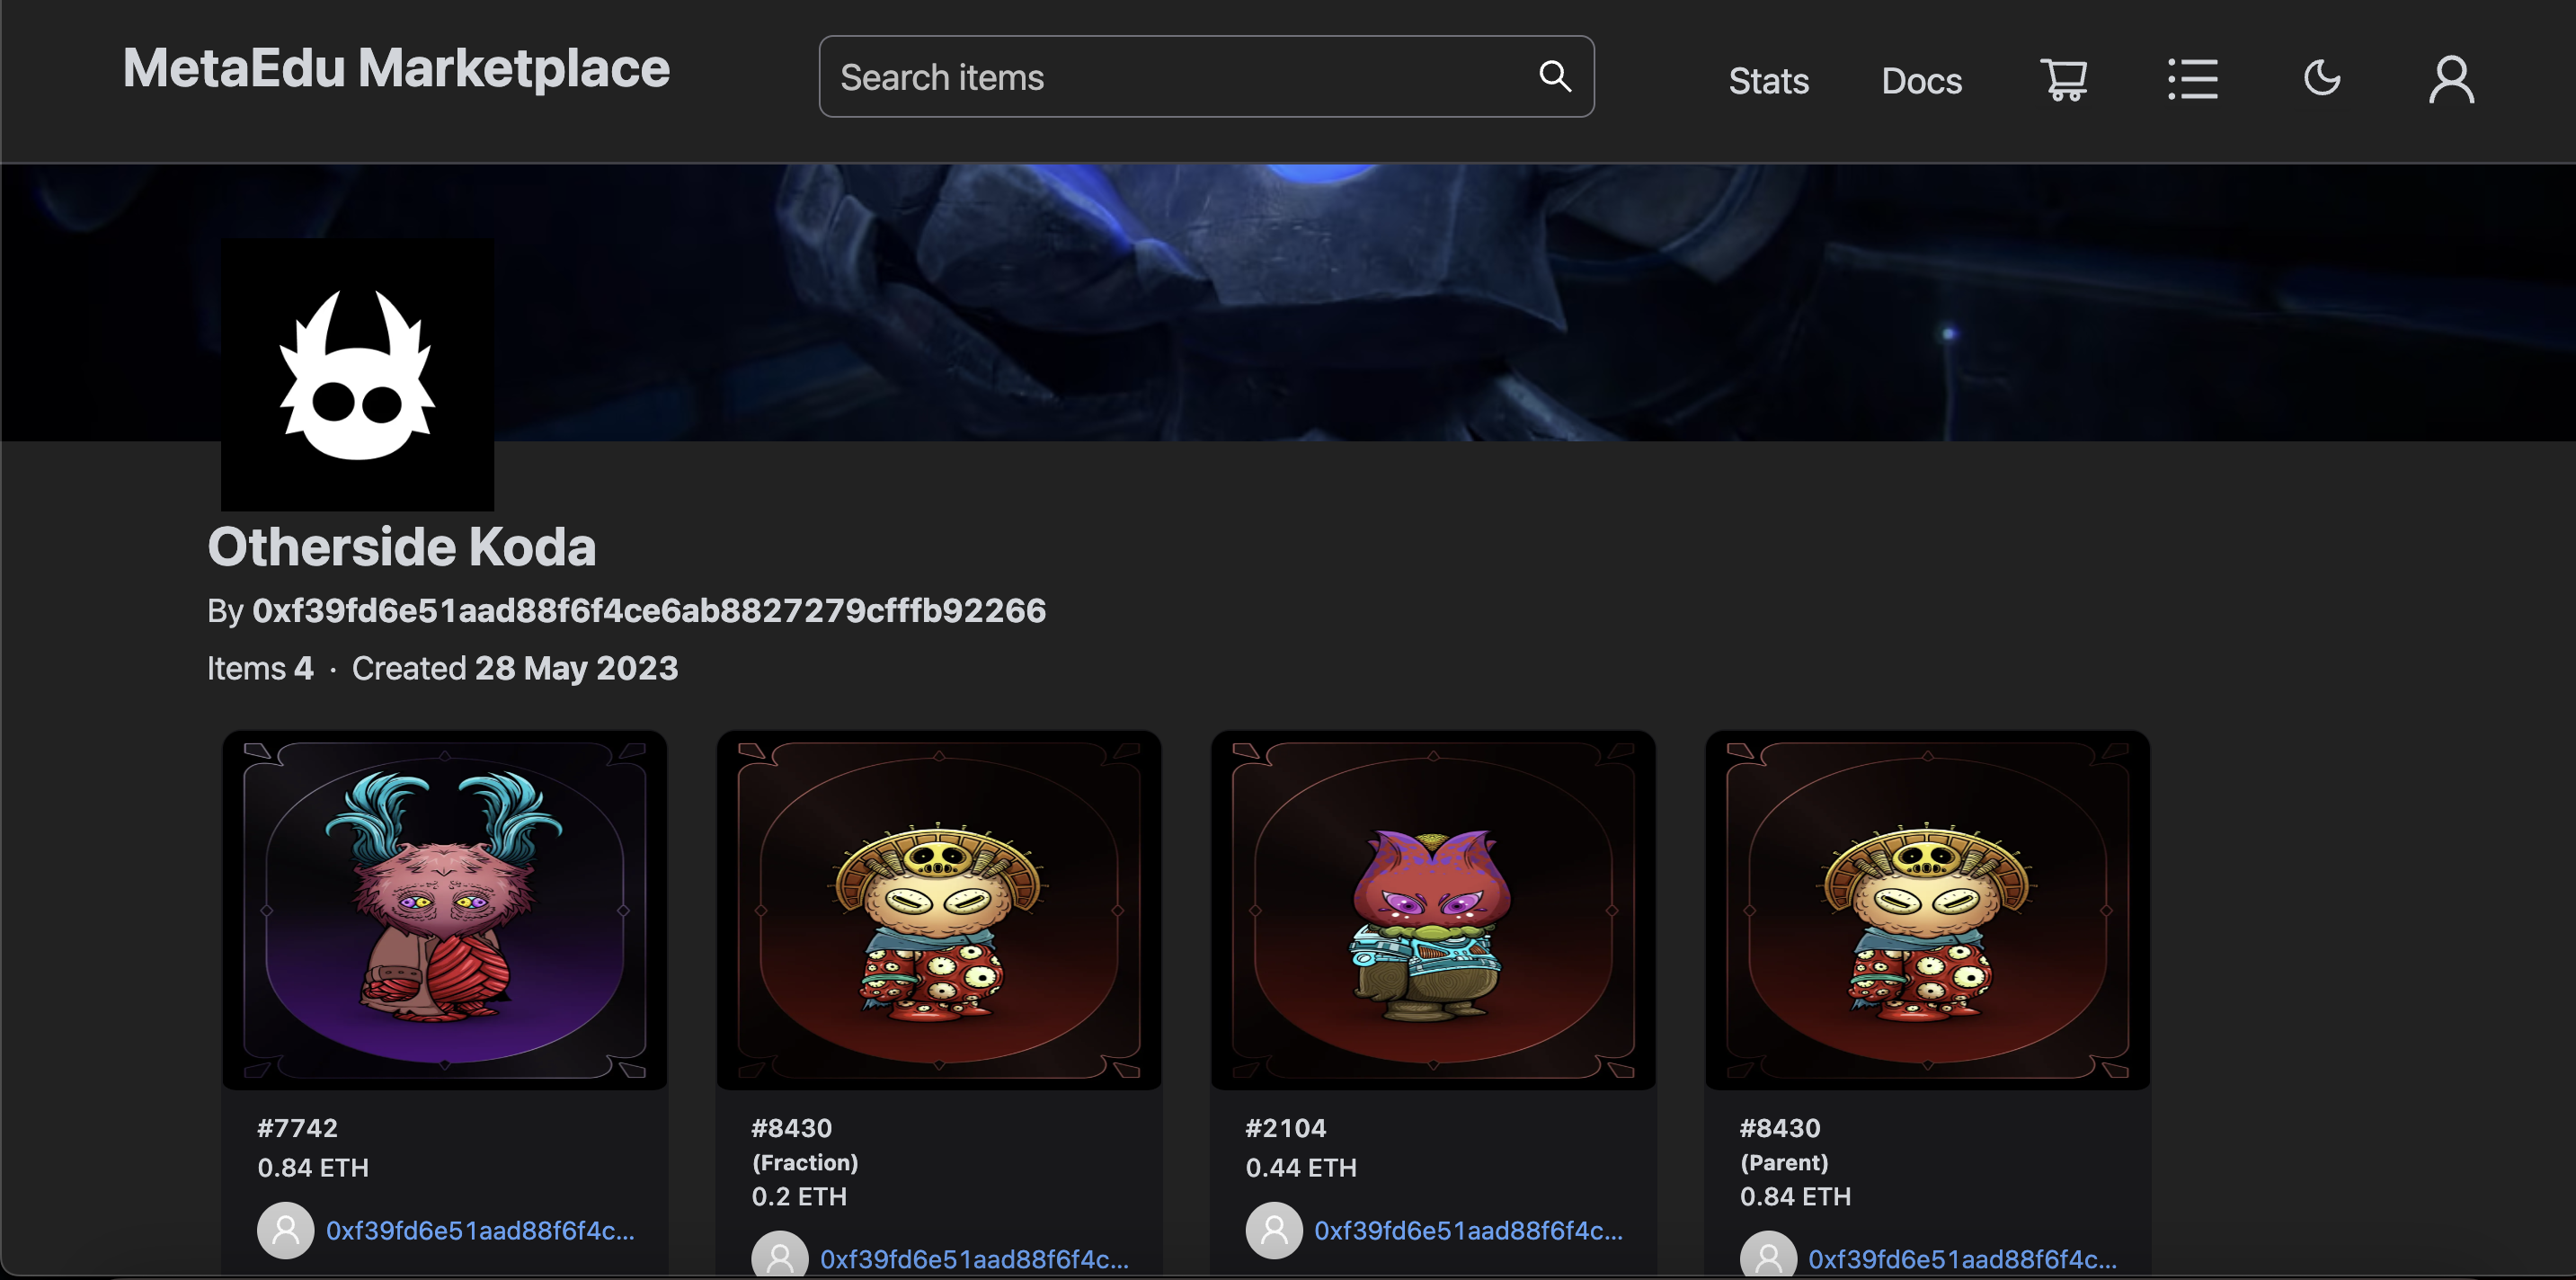
\includegraphics[scale=0.3]{gambar/img-frontend-collection.png}
  \caption{Halaman detail koleksi}
  \label{fig:CollectionDetail}
\end{figure}

Halaman detail koleksi berisi daftar token yang terkait dengan kolesi tersebut.

\subsection{Halaman Statistik}
\begin{figure} [H] \centering
  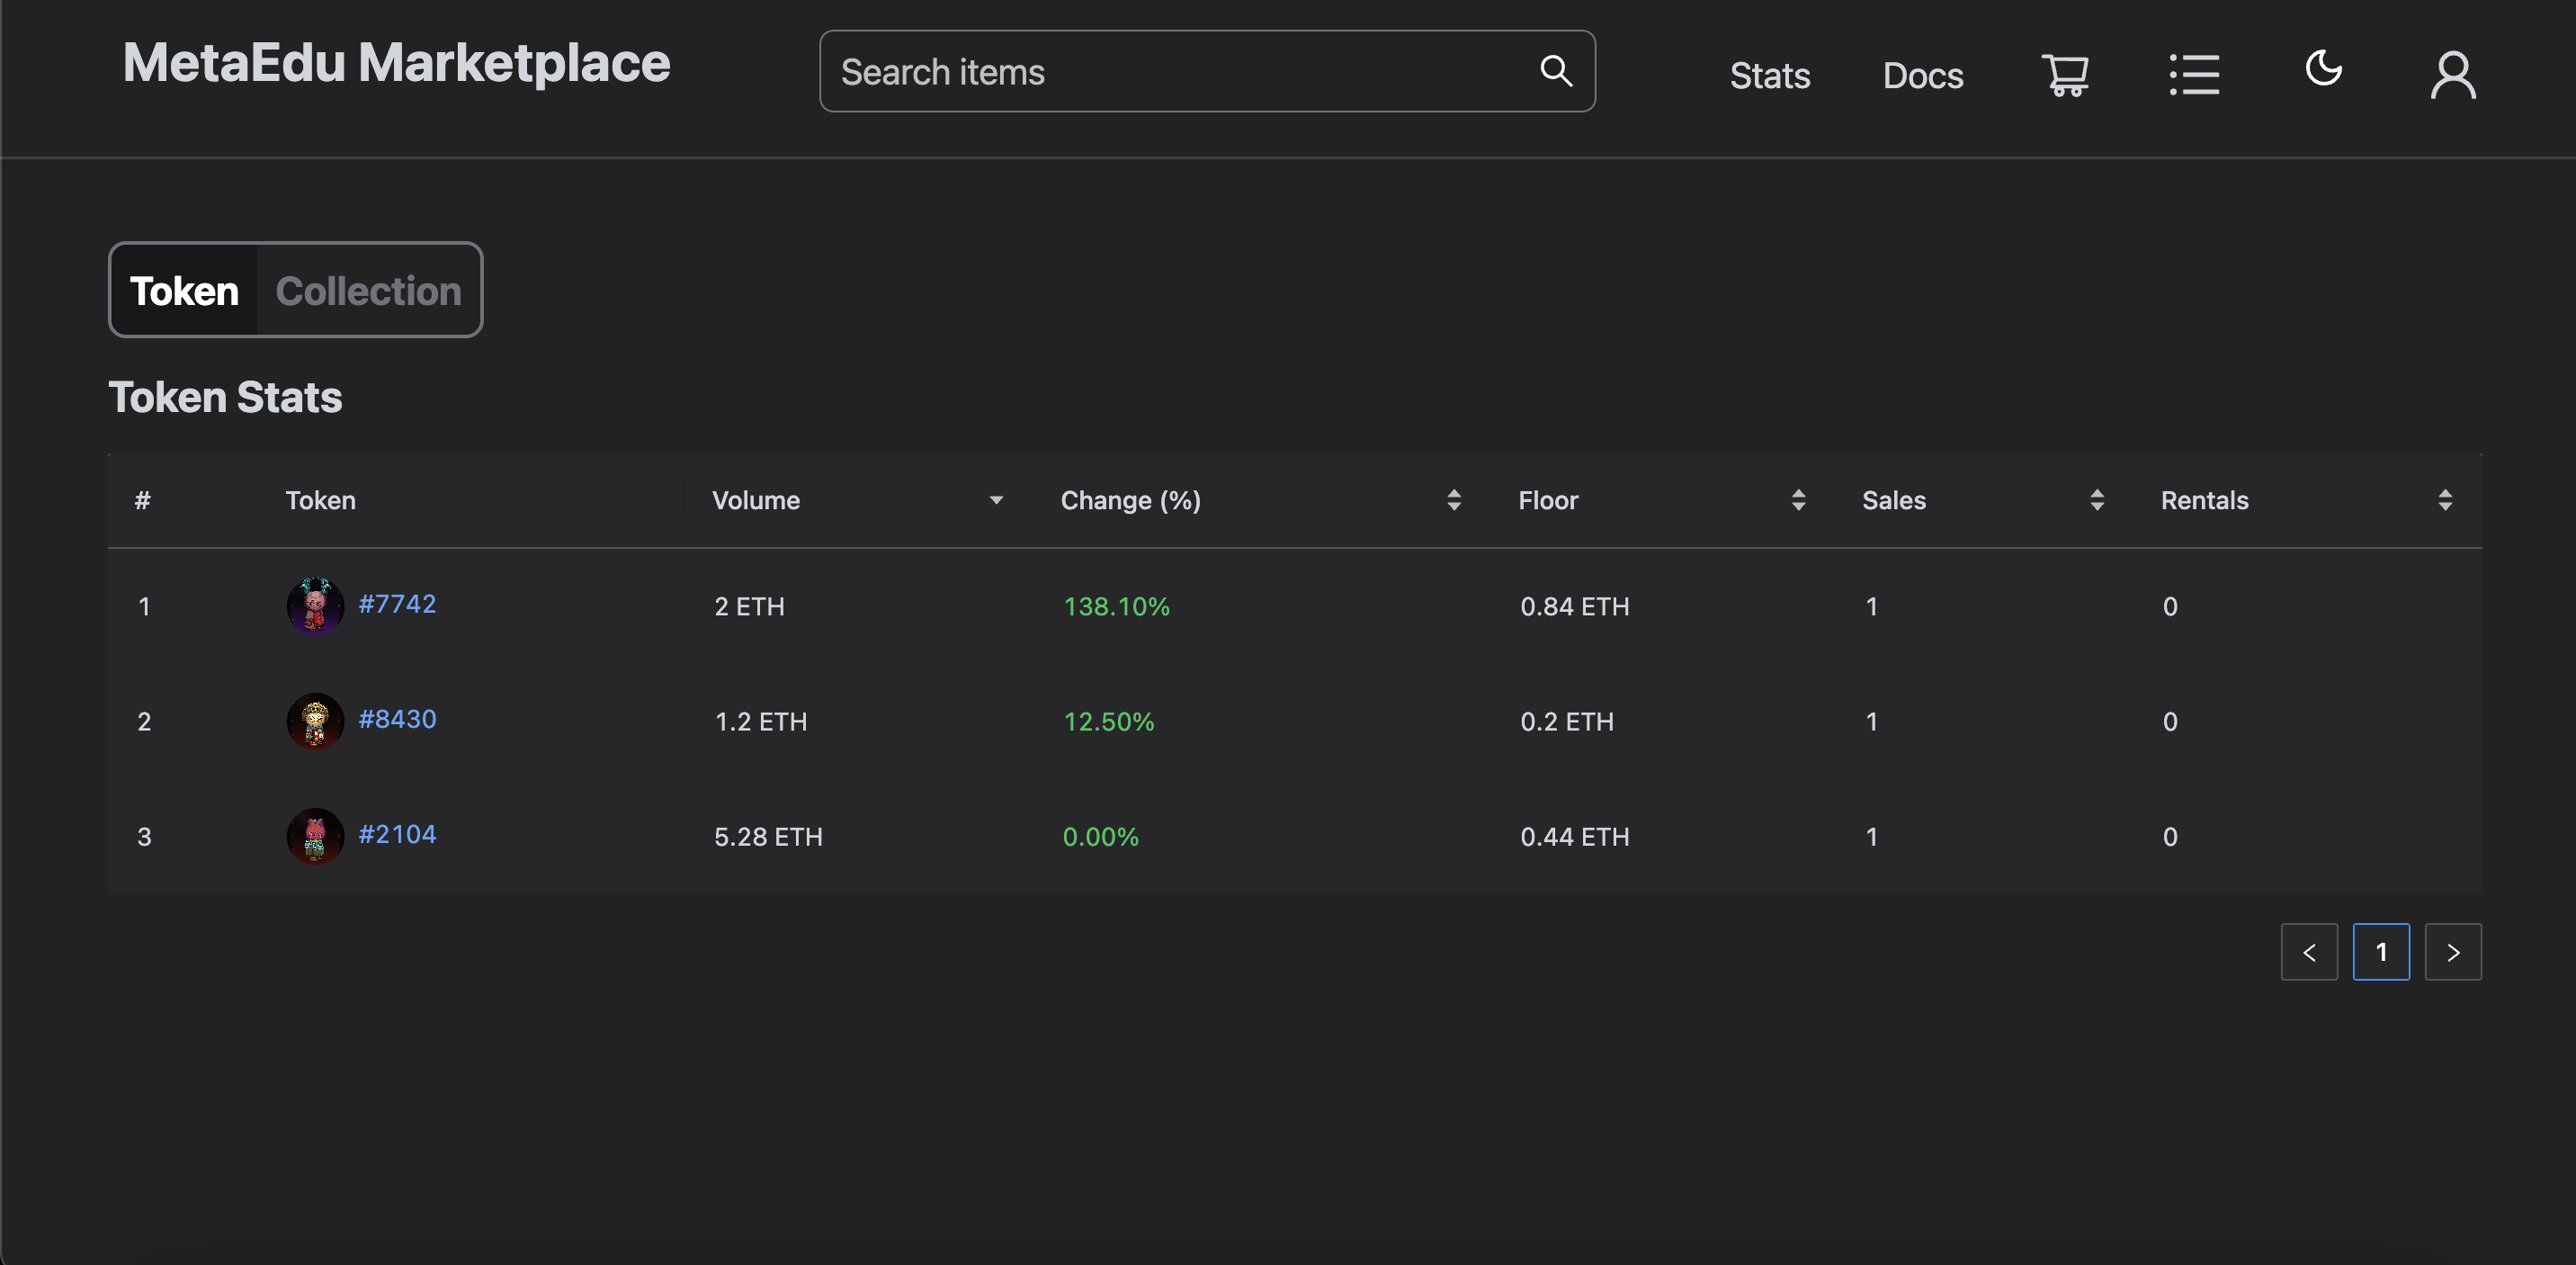
\includegraphics[scale=0.3]{gambar/img-frontend-stats.png}
  \caption{Halaman statistik}
  \label{fig:TokenStats}
\end{figure}

Halaman statistik berisi daftar token dan koleksi yang diurutkan berdasarkan parameter seperti \emph{Volume}, perubahan harga, \emph{floor} / harga terbawah, jumlah penjualan dan jumlah penyewaan.

\subsection{Halaman Dokumentasi}
\begin{figure} [H] \centering
  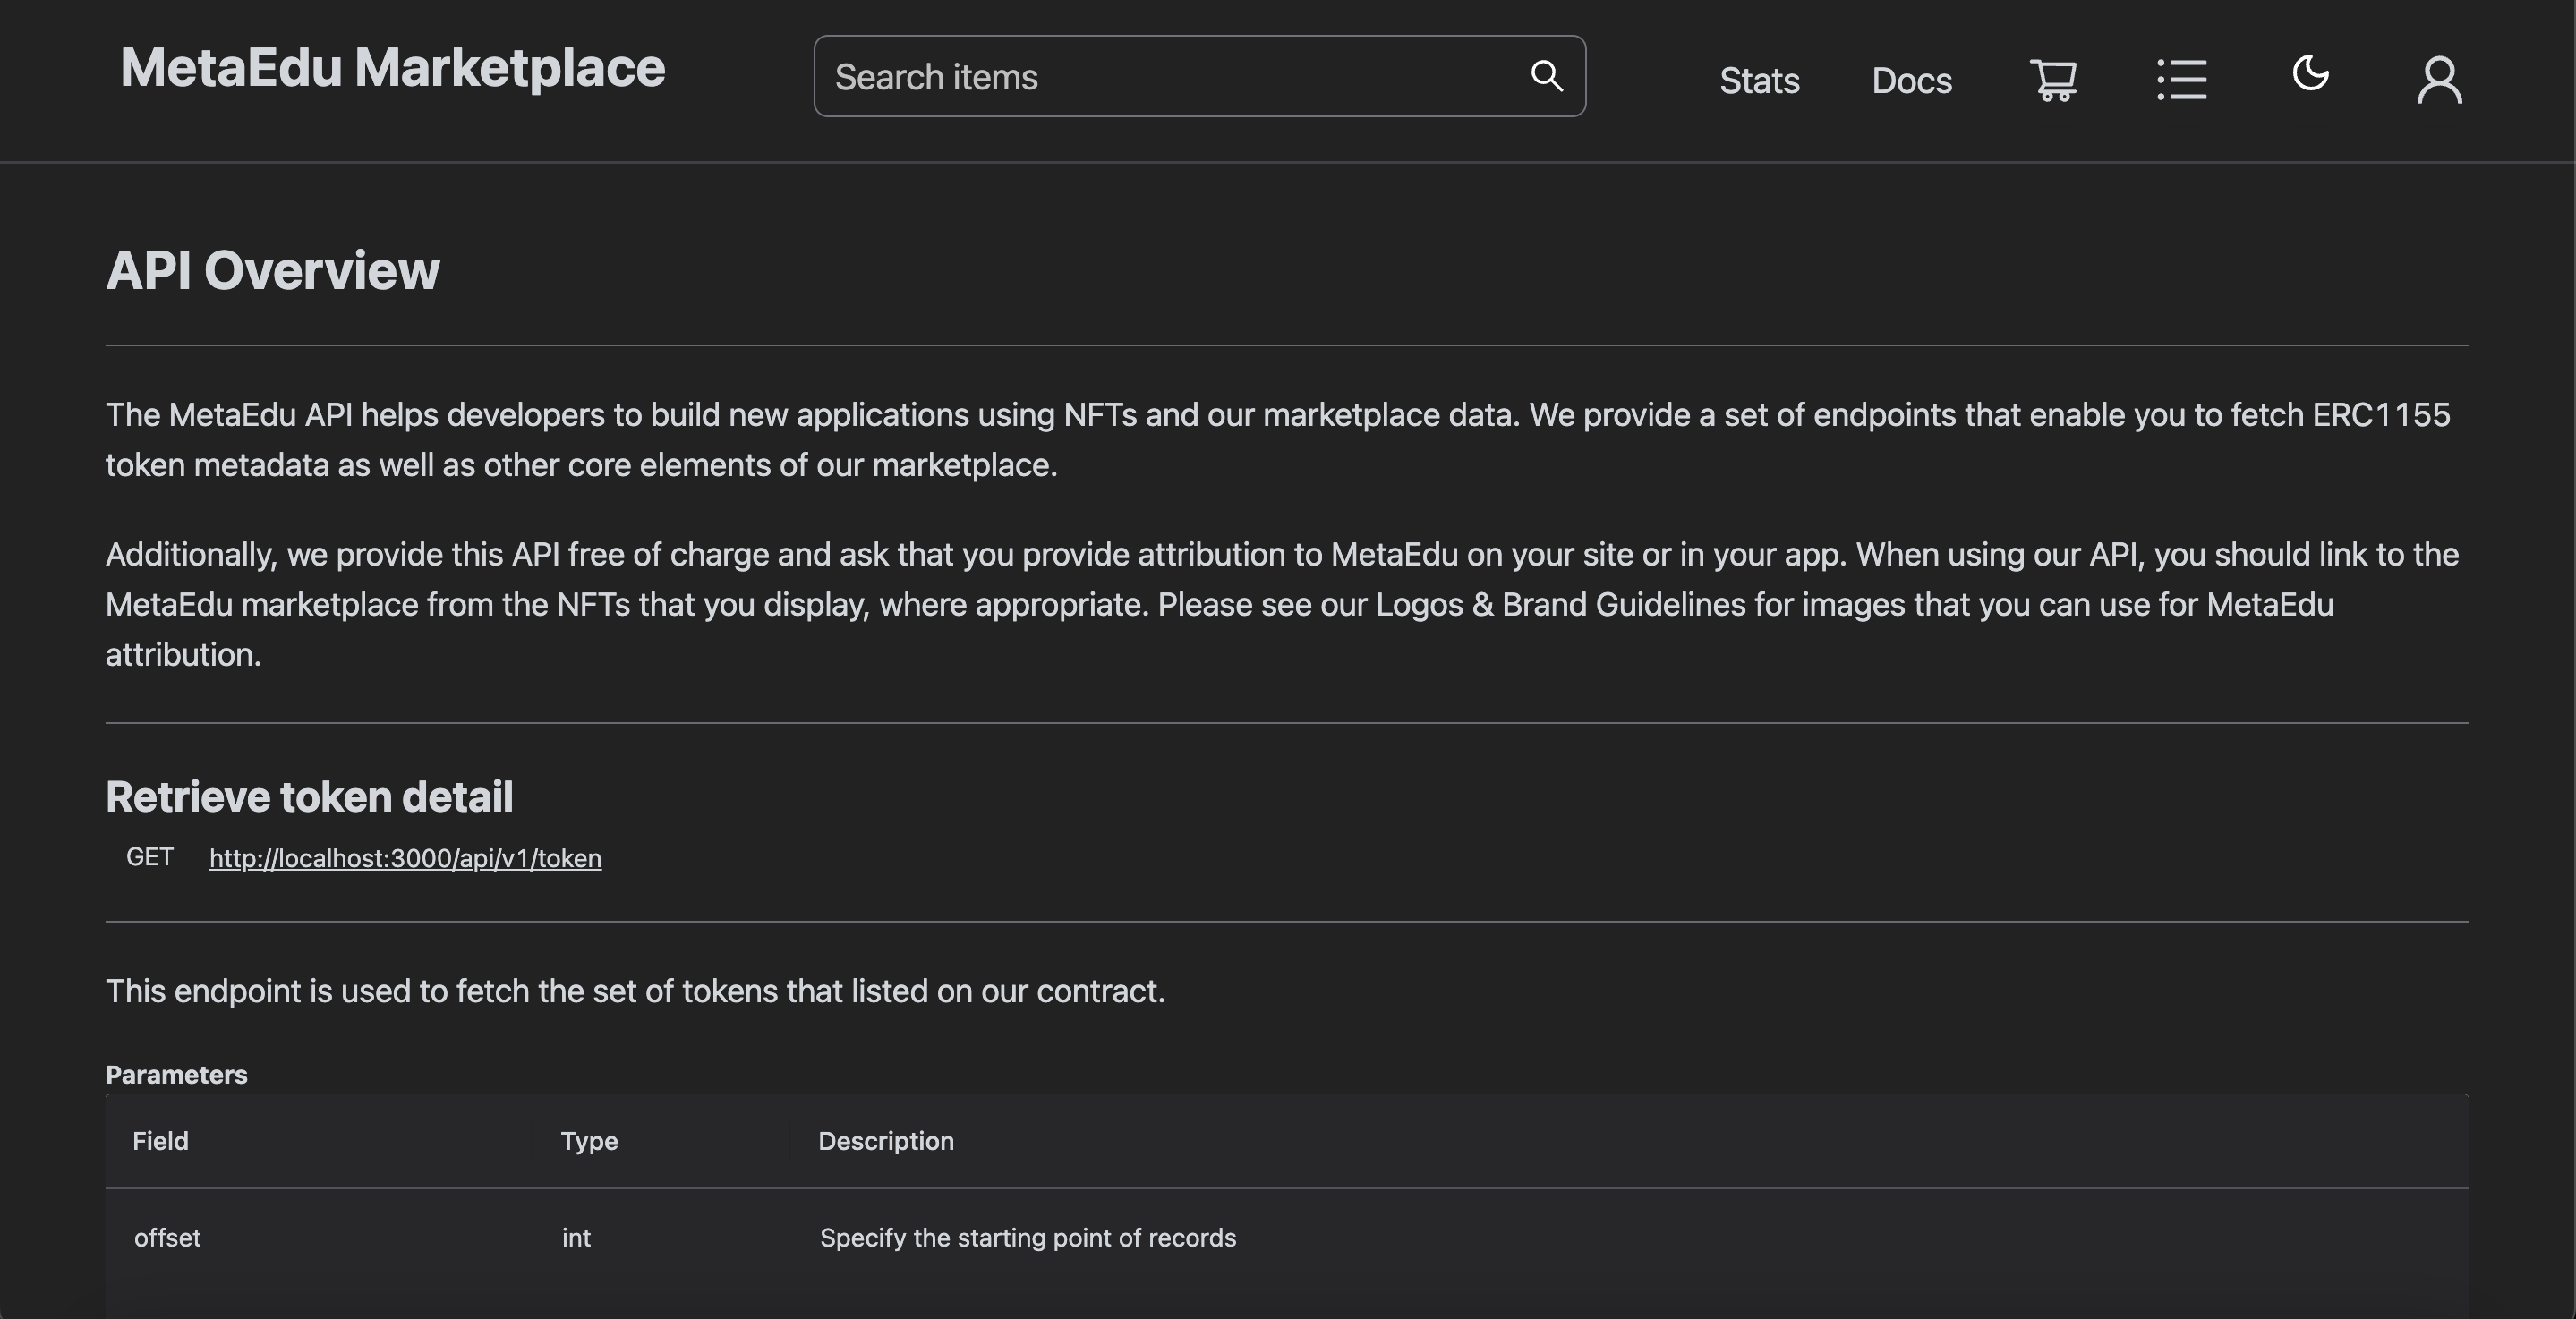
\includegraphics[scale=0.3]{gambar/img-frontend-api.png}
  \caption{Halaman dokumentasi}
  \label{fig:Docs}
\end{figure}

Halaman dokumentasi berisi informasi mengenai \emph{API} yang disedikan untuk \emph{platform} lain dapat memanfaatkan data dari \emph{NFT Marketplace} ini seperti data token, kepemilikan, dan penyewaan.

\subsection{API Marketplace} 

API Marketplace digunakan untuk memperoleh berbagai data dari \emph{database} yang pada \emph{web marketplace} maupun \emph{metaverse}.

\begin{figure} [H] \centering
  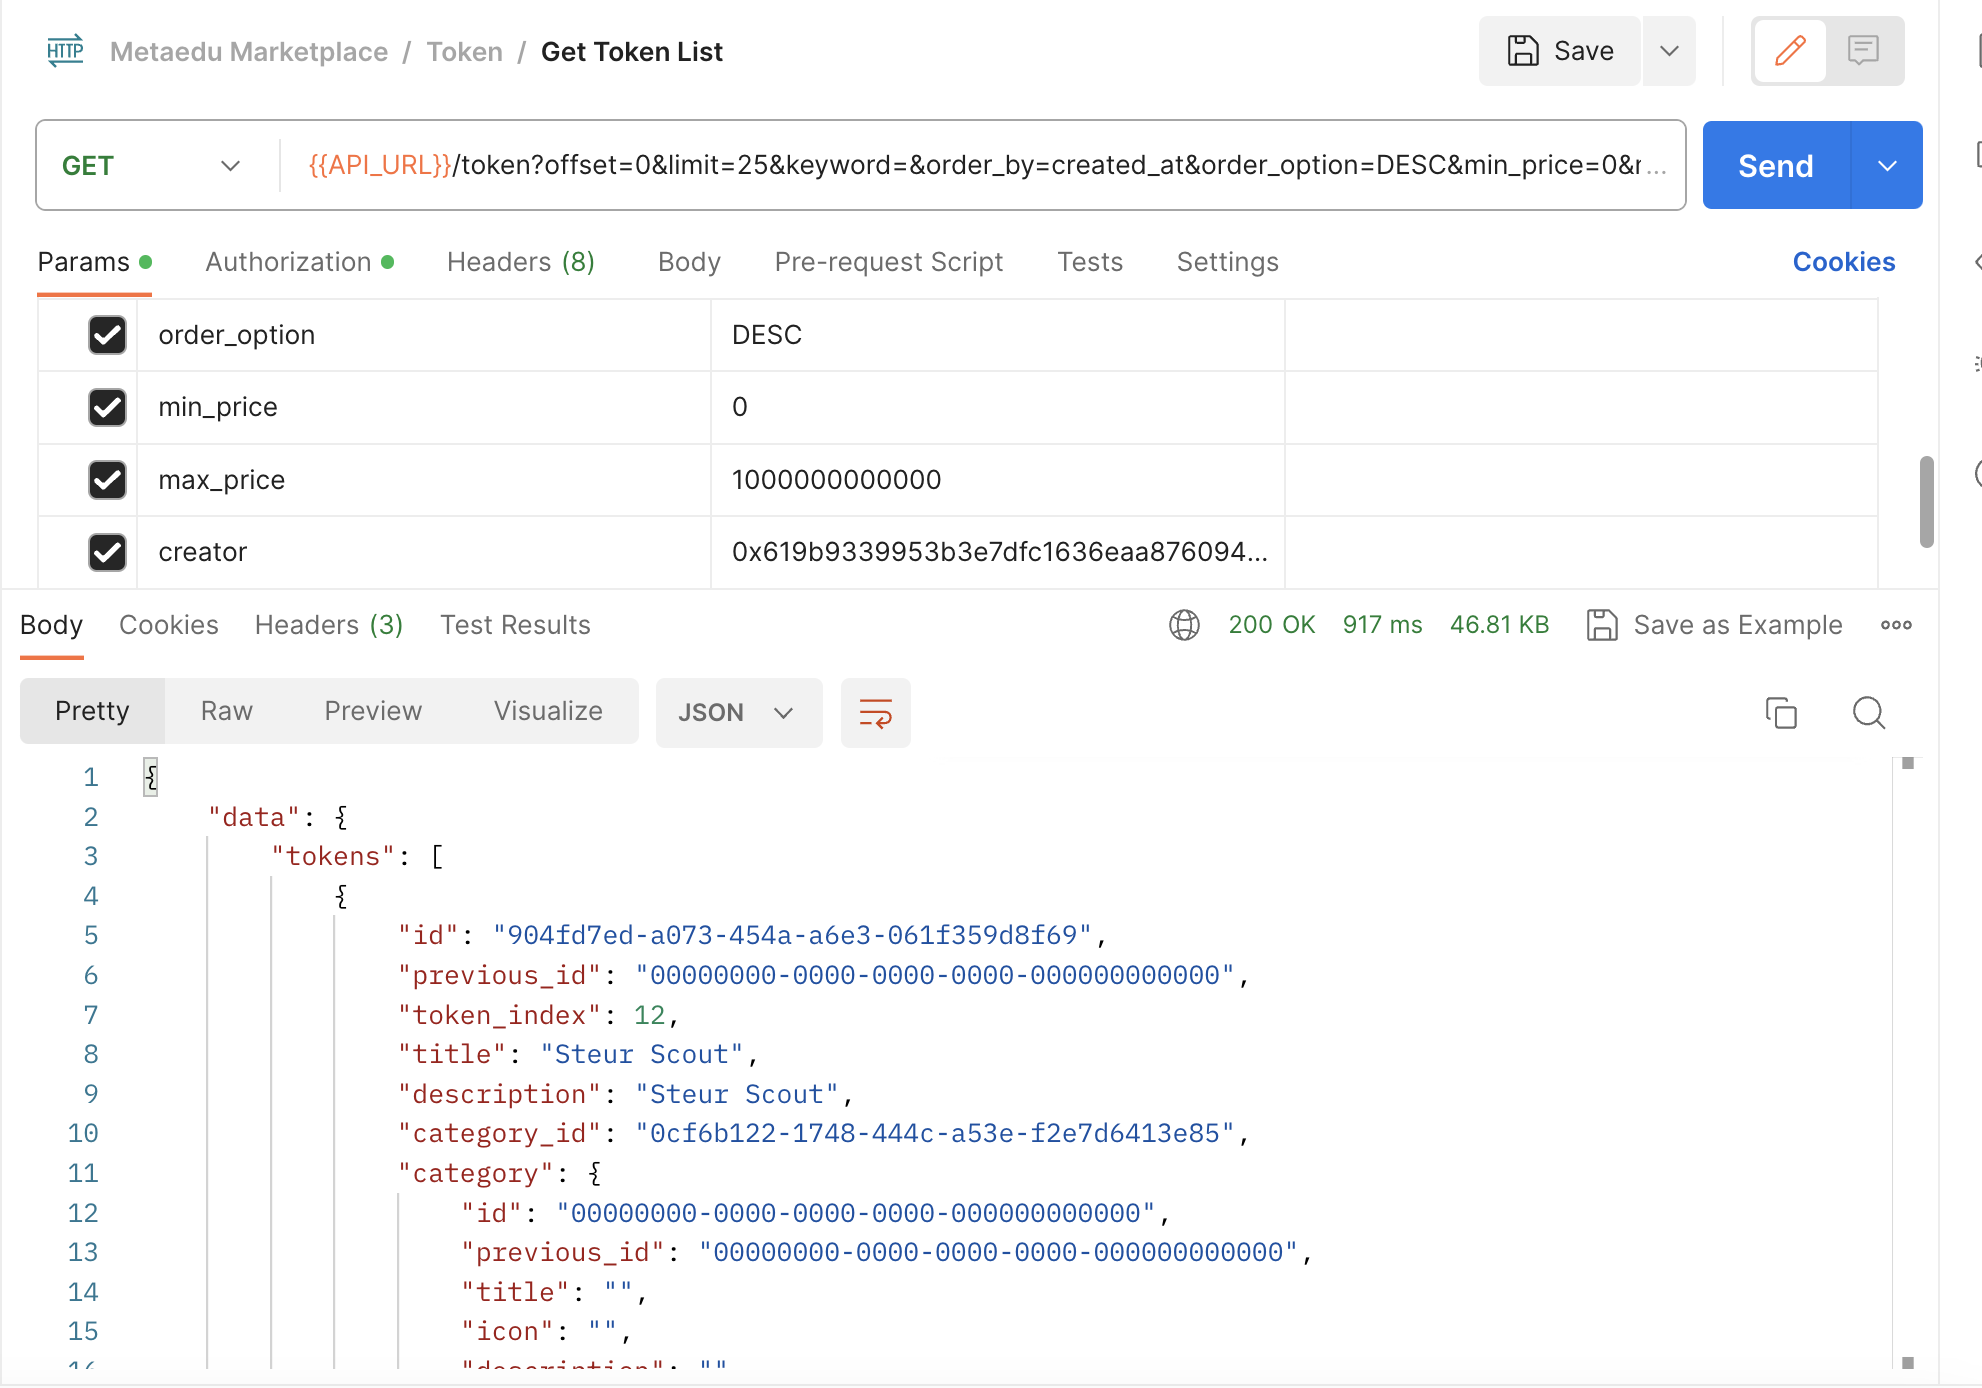
\includegraphics[scale=0.3]{gambar/img-api-tokens.png}
  \caption{\emph{API token} }
  \label{fig:APITokens}
\end{figure}

\emph{API} token memiliki \emph{prefix \textbf{\textbackslash token}} dan digunakan memperoleh seluruh data token yang disimpan dalam \emph{table tokens}. 

\begin{figure} [H] \centering
  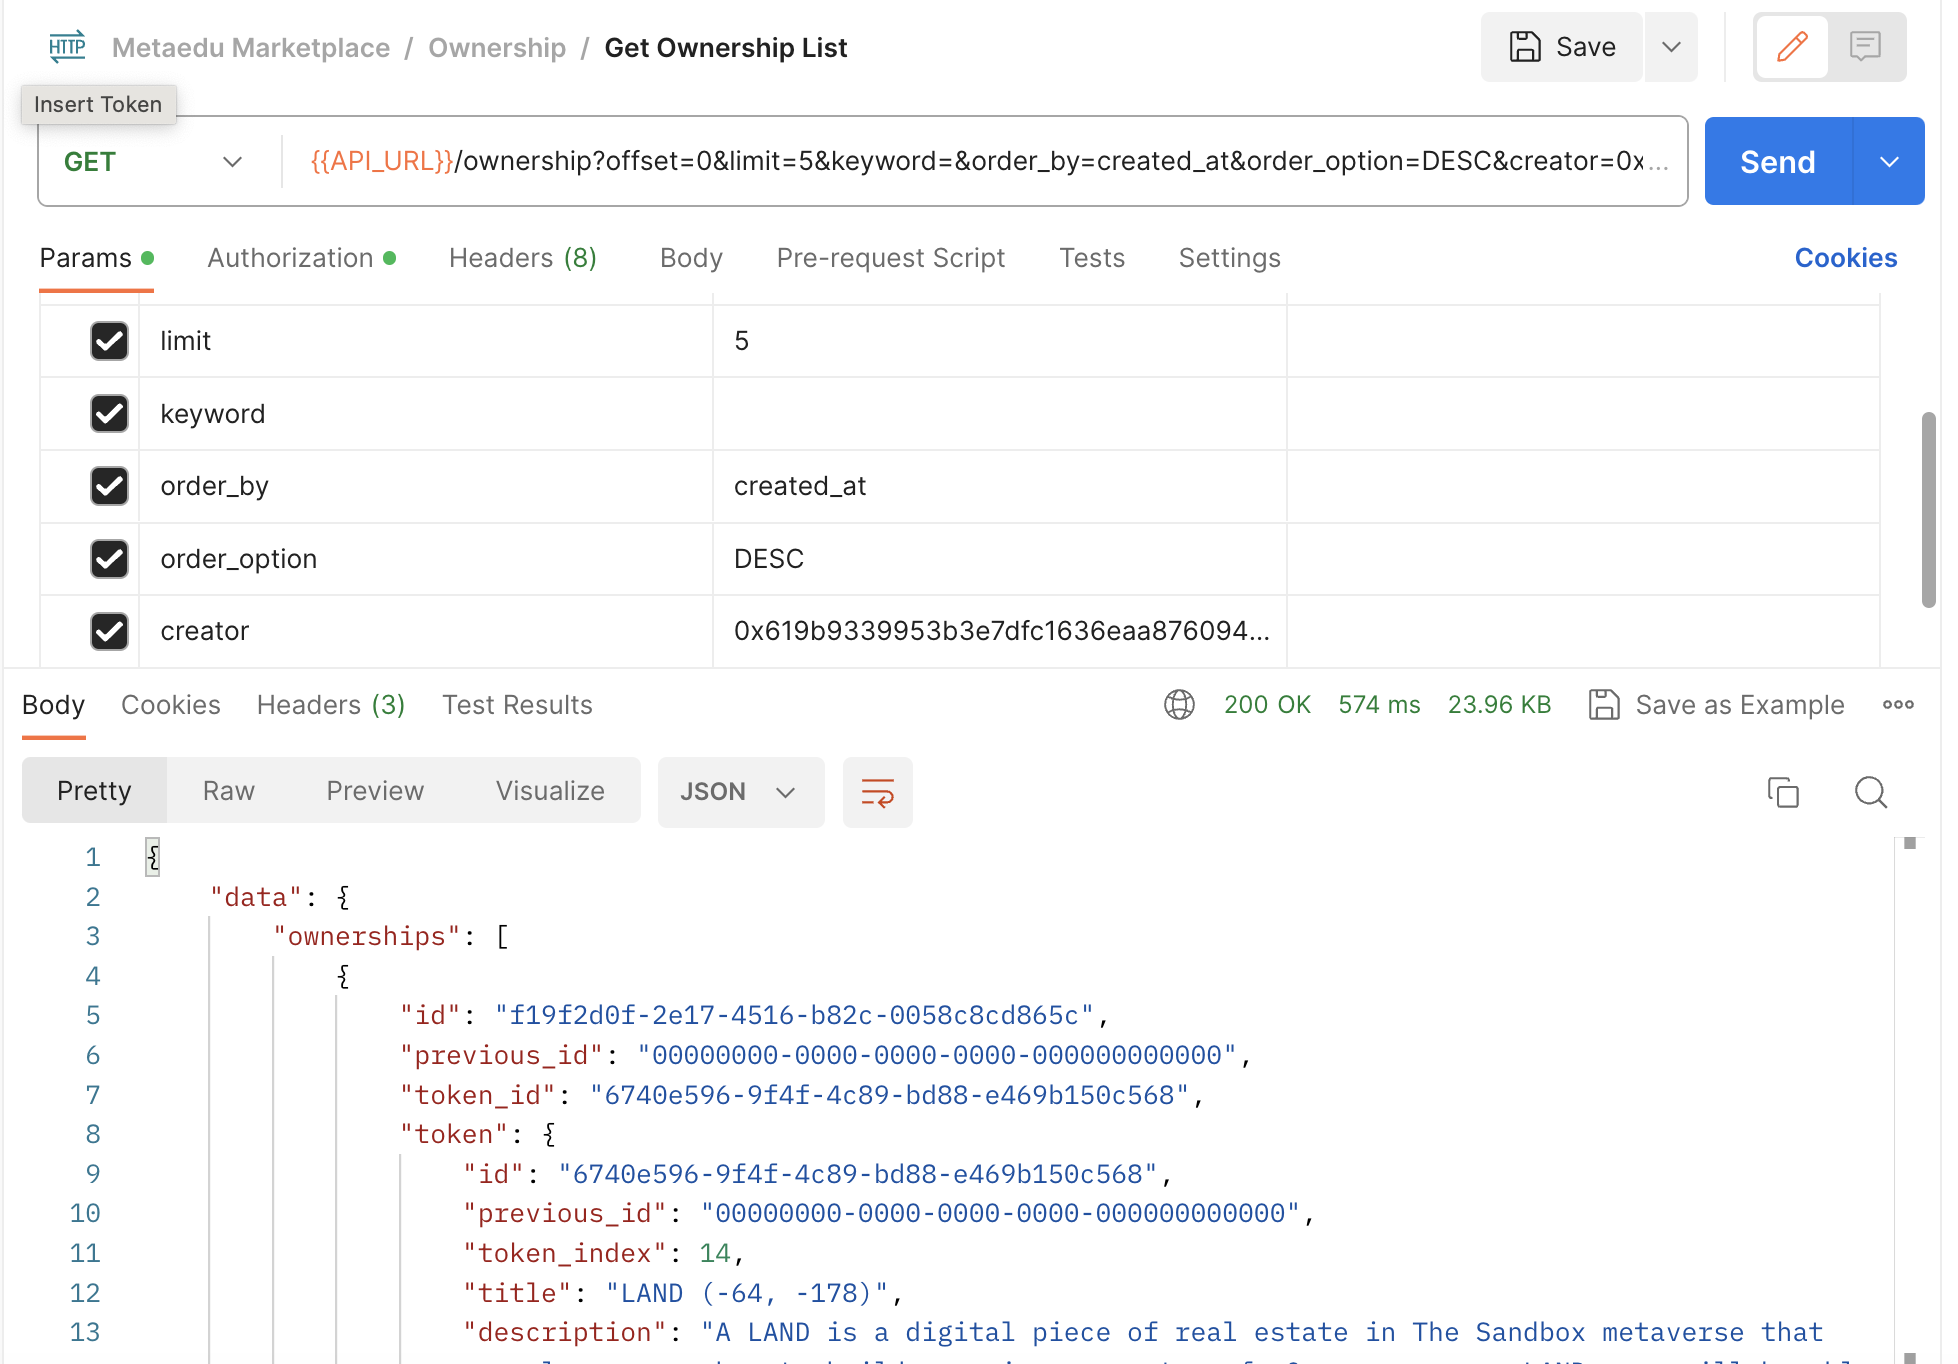
\includegraphics[scale=0.3]{gambar/img-api-ownerships.png}
  \caption{\emph{API token} }
  \label{fig:APIOwnerships}
\end{figure}

\emph{API} ownerships memiliki \emph{prefix \textbf{\textbackslash ownership}} dan digunakan memperoleh seluruh data kepemilikan token oleh pengguna yang disimpan dalam \emph{table ownerships}. 

\begin{figure} [H] \centering
  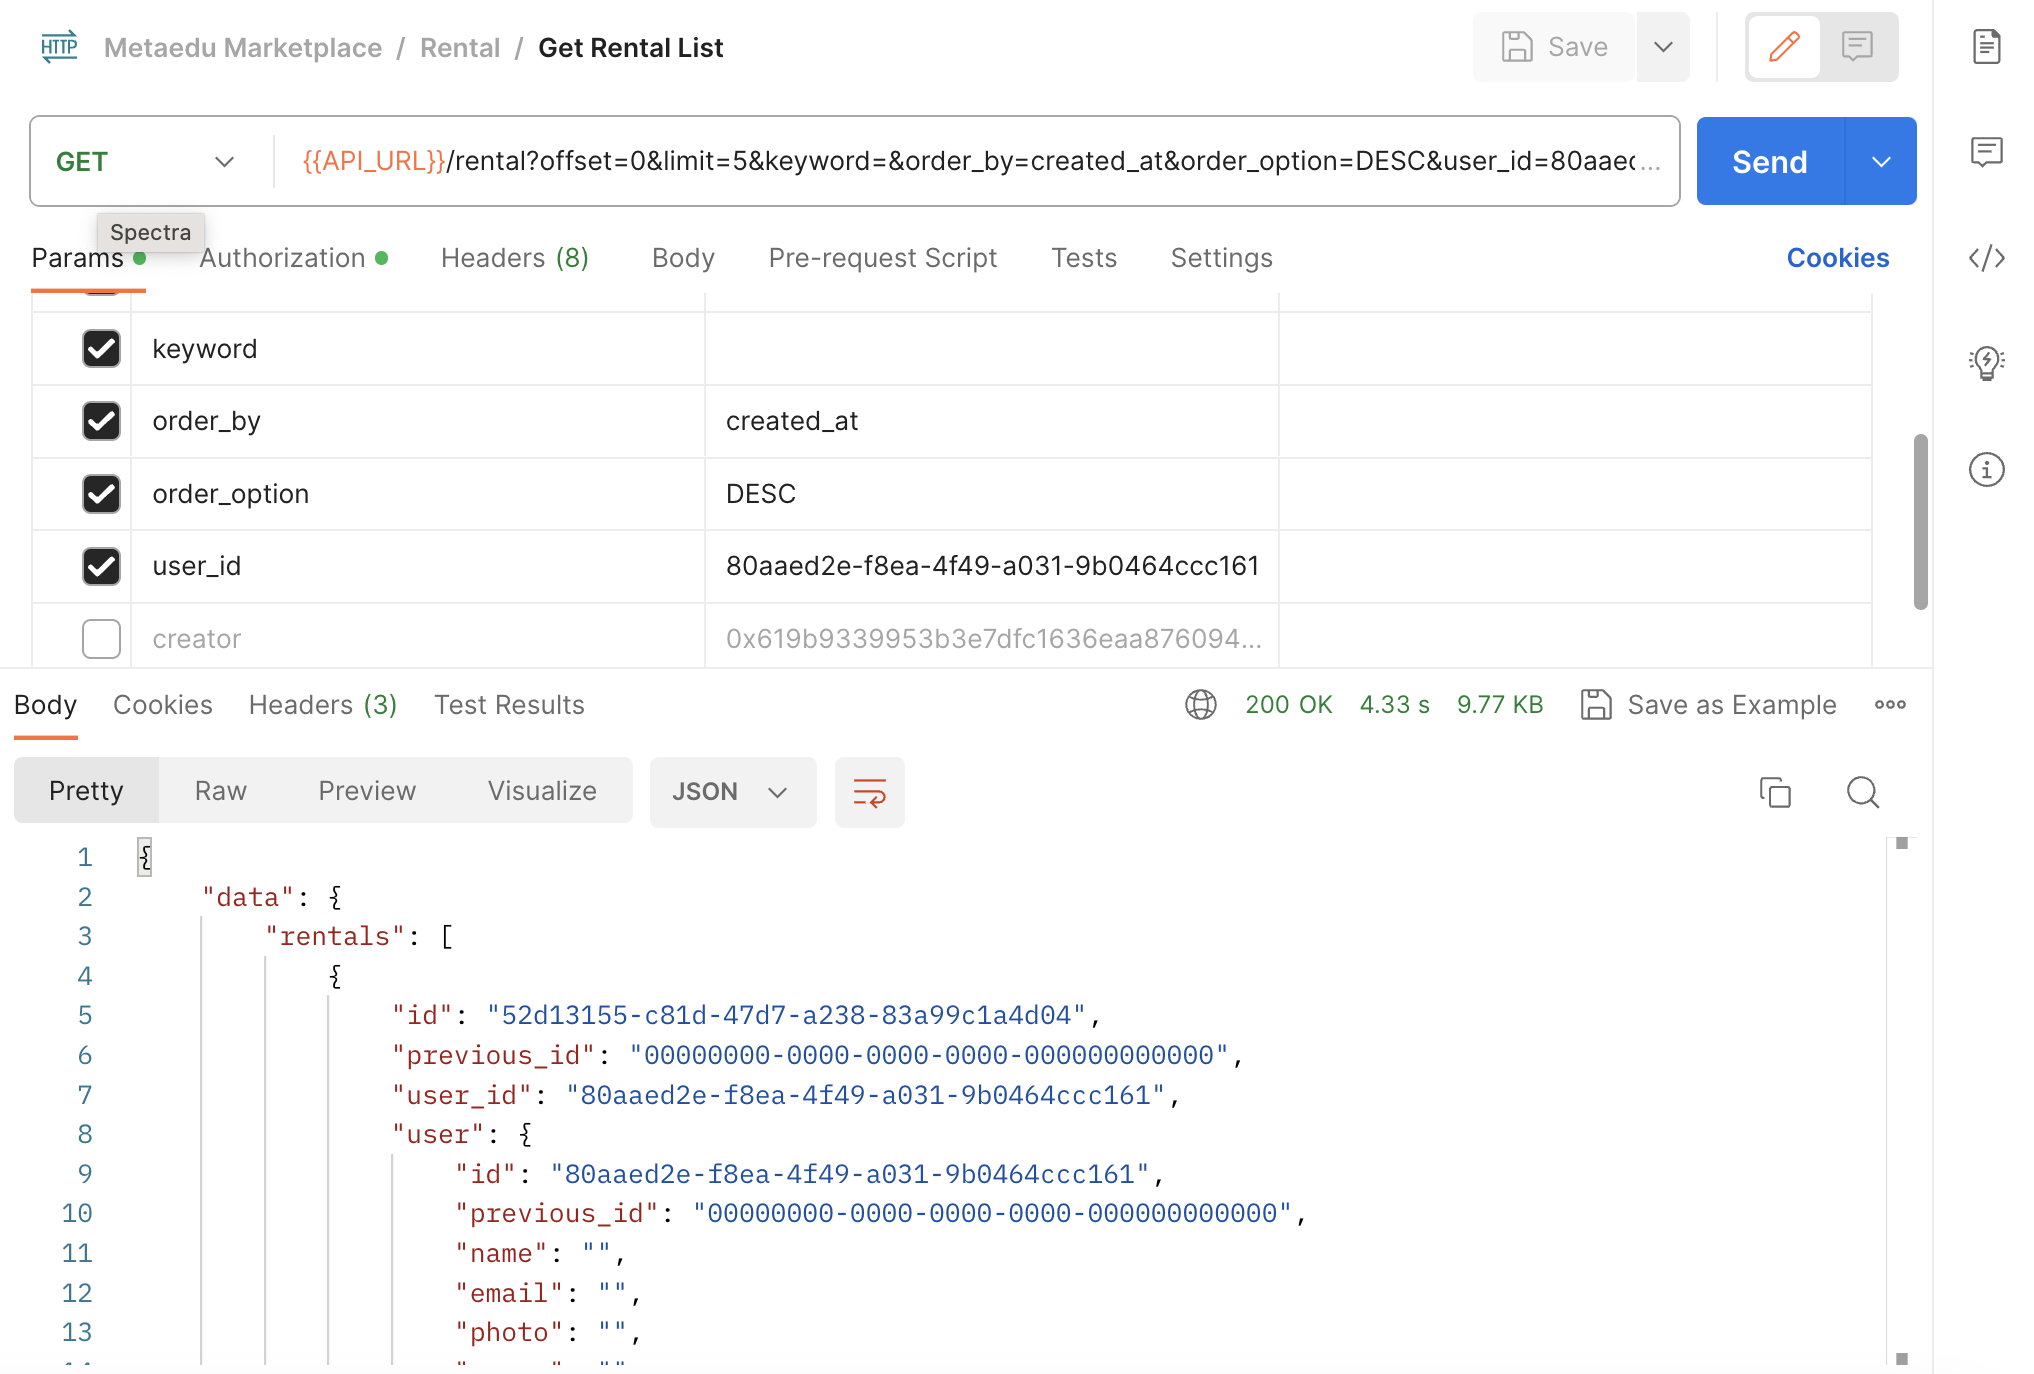
\includegraphics[scale=0.3]{gambar/img-api-rentals.png}
  \caption{\emph{API rental} }
  \label{fig:APIRentals}
\end{figure}

\emph{API} rentals memiliki \textbf{\textbackslash rental} dan digunakan memperoleh seluruh data peminjaman token yang disimpan dalam \emph{table rentals}. 

\begin{figure} [H] \centering
  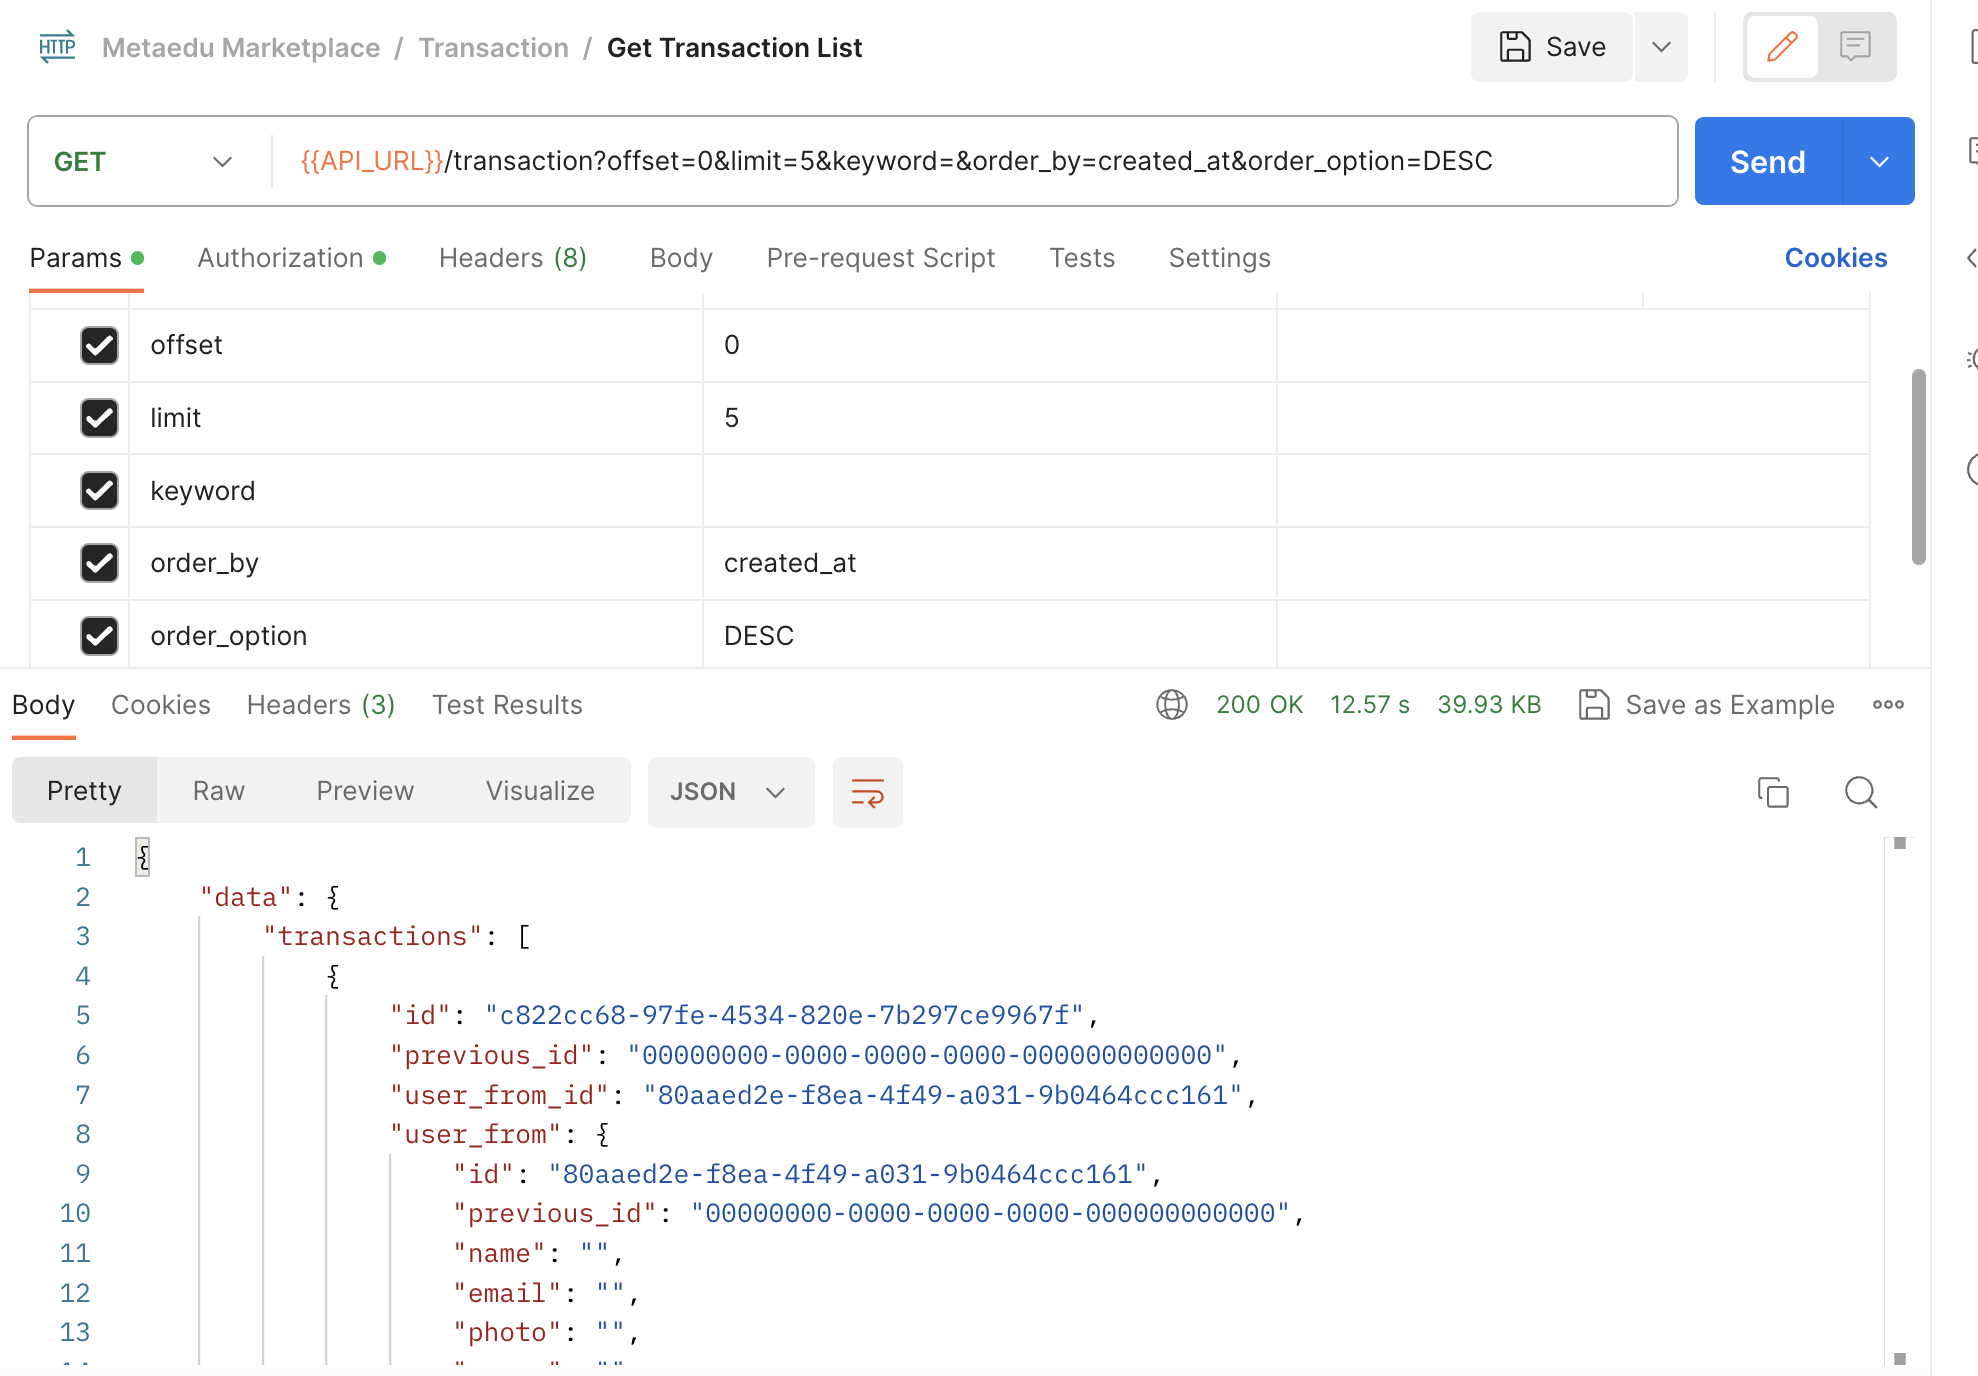
\includegraphics[scale=0.3]{gambar/img-api-transactions.png}
  \caption{\emph{API transaction} }
  \label{fig:APITransactions}
\end{figure}

\emph{API} transactions memiliki \textbf{\textbackslash transaction} dan digunakan memperoleh seluruh data transaksi baik penjualan maupun penyewaan token disimpan dalam \emph{table transactions}. 

\begin{figure} [H] \centering
  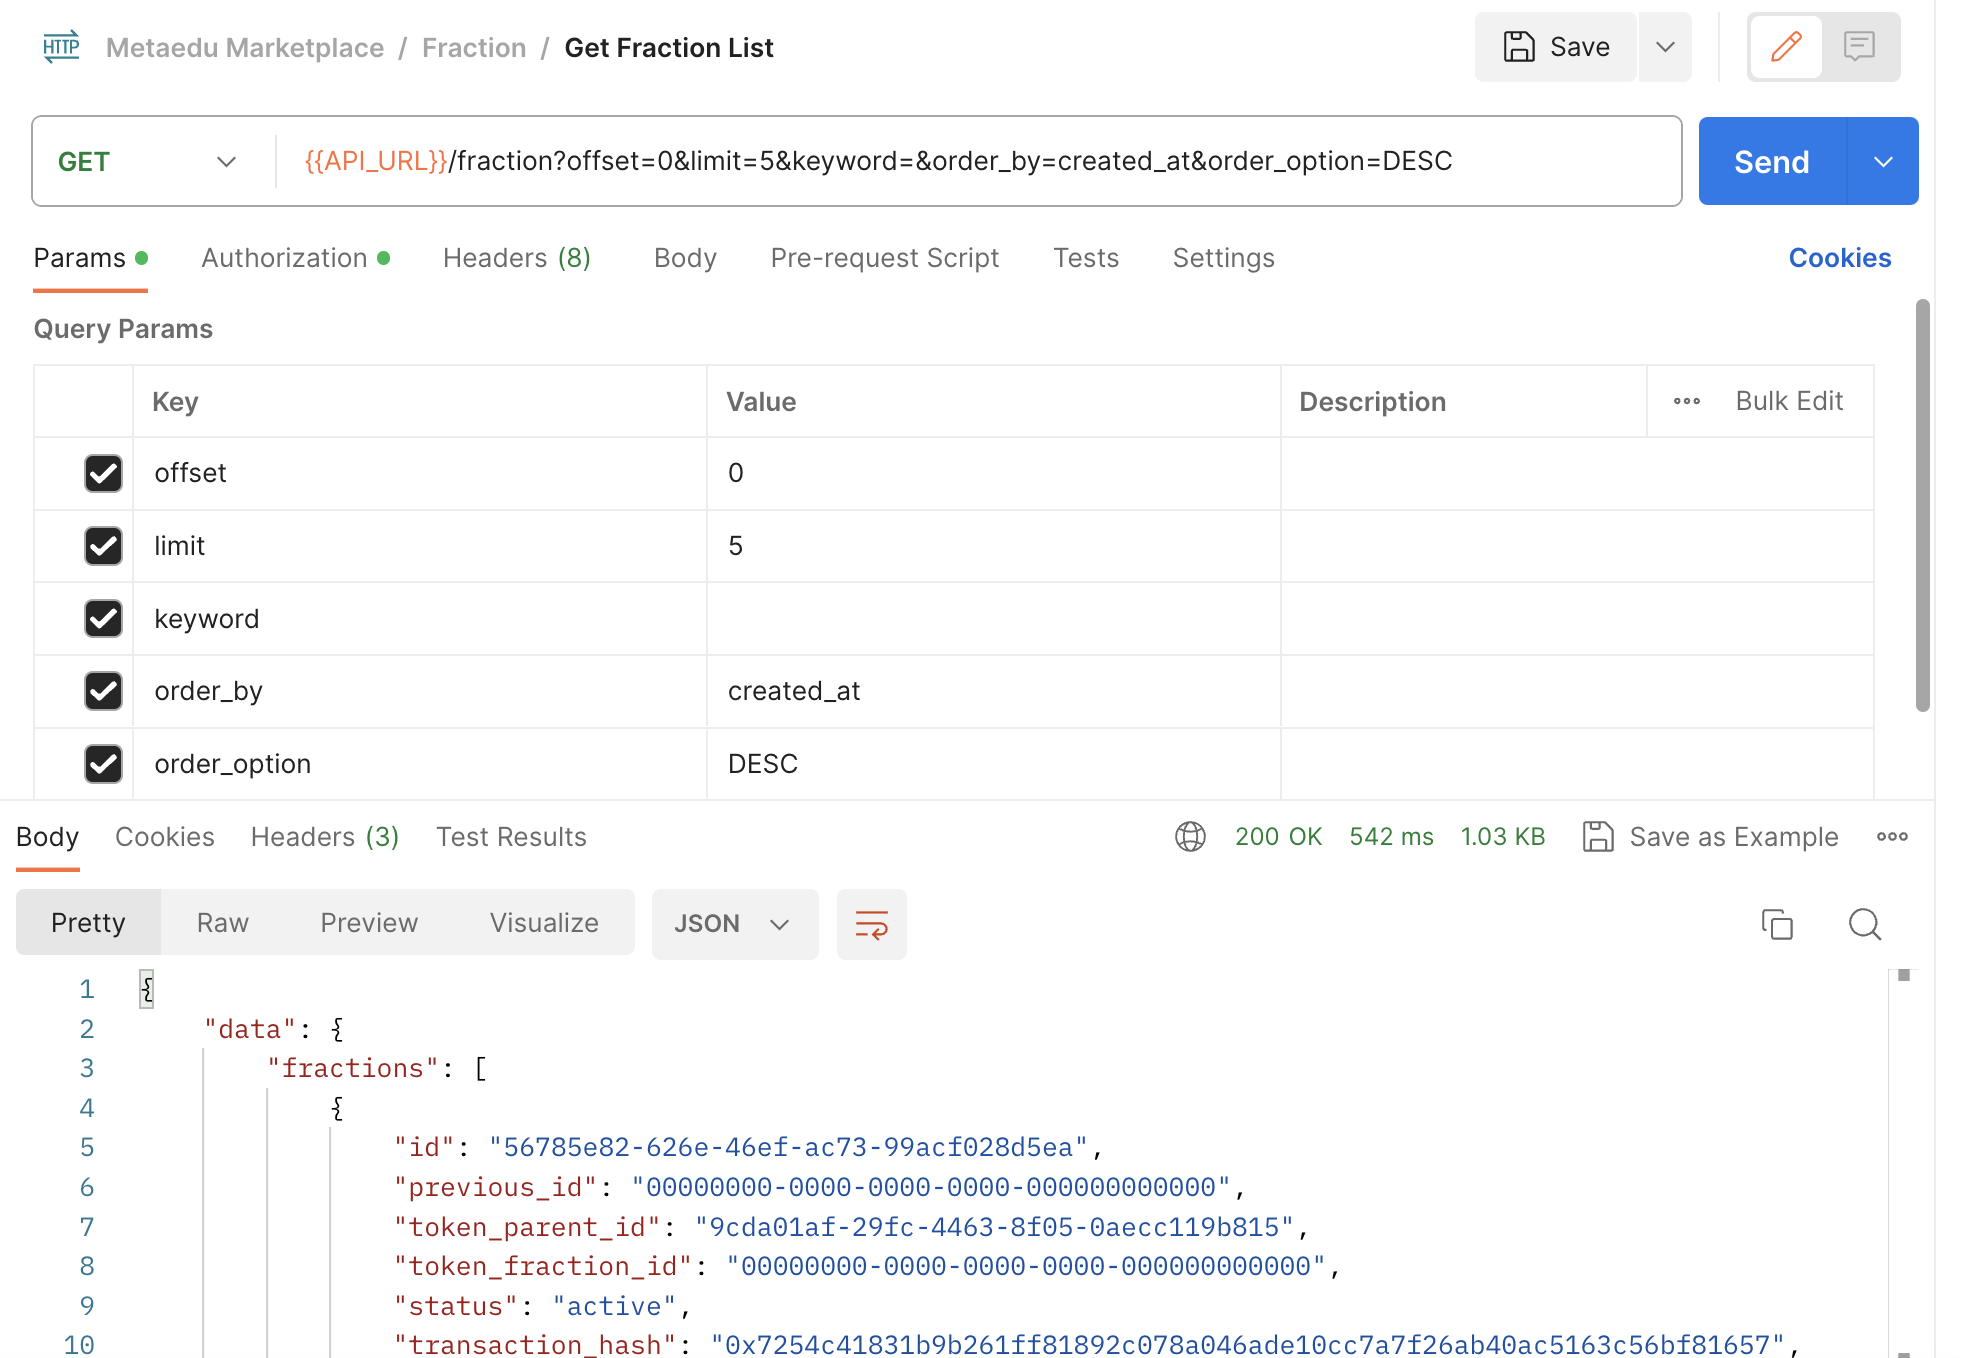
\includegraphics[scale=0.3]{gambar/img-api-fractions.png}
  \caption{\emph{API fraction} }
  \label{fig:APIFractions}
\end{figure}

\emph{API} fractions memiliki \textbf{\textbackslash fractions} dan digunakan memperoleh seluruh data \emph{fractionslization} yang disimpan dalam \emph{table fractions}. 

\emph{API-API} di atas dikembangkan supaya dapat diakses se-fleksibel mungkin sehingga menyesuaikan kebutuhan dari aplikasi \emph{frontend} dan \emph{platform metaverse} yang ingin terintegrasi. Dikarenakan hal tersebut terdapat parameter-parameter yang dapat ditambahkan dalam mengakses \emph{API} tersebut sebagai berikut

\begin{longtable}{|c|c|}
  \caption{Parameter \emph{API}}
  \label{tb:APIParameters}                                   \\
  \hline
  \rowcolor[HTML]{C0C0C0}
  \textbf{Parameter} &  \textbf{Deskripsi} \\
  \hline
  Keyword            & Memfilter data Berdasarkan kunci dari tertentu                                        \\
  Offset             & Menampilkan data dari index tertentu                           \\
  Limit            & Membatasi data                                                           \\
  Order By            & Mengurutkan data berdasarkan \emph{field} tertentu                                 \\
  Order Option        & Mengurutkan data berdasarkan index rendah ke tinggi atau sebaliknya                              \\
  Creator              & Memfilter data berdasarkan \emph{address} pemilik atau penyewa \emph{token}                                                                             \\
  User          & Memfilter data berdasarkan \emph{address} pengguna \\
  
  \hline
\end{longtable}


Pada penelitian ini dipaparkan hasil pengujian melalui aplikasi \emph{Front End} yang memicu pemanggilan \emph{function}-\emph{function} dalam \emph{smart contract}. Hasil dari pengujian ini diharapkan bahwa data-data berupa \emph{token}, \emph{ownership}, \emph{rental} sesuai dengan \emph{flow}-nya. \emph{Ether} yang dikirimkan sesuai dengan \emph{EOA} terkait transaksi tertentu sesuai. Selain itu selama pengujian berlangsung \emph{gass fee} yang diestimasikan dan diperlukan akan di data untuk mengetahui masing-masing \emph{gass fee} pada masing-masing pemanggilan \emph{function}. Hal ini menjadi penting dikarenakan merupakan suatu kondisi yang merepresentasikan bahwa \emph{smart contract} yang dikembangkan efisien.

\section{Pengujian Fitur-Fitur Utama Marketplace}
\label{sec:skenariopengujian}

Pengujian ini berfokus terhadap fitur-fitur utama pada \emph{marketplace} dalam 3 \emph{flow} yaitu pembelian, penyewaan, pembagian kepemilikan dimana yang menjadi fokus utama adalah kepemilikan NFT setelah setiap transaksi dilakukan, ketuntungan maupuan potongan yang dihasilkan selama transaksi berlangsung dan efektifias fungsi melalui gas yang dihasilkan.  \emph{Wallet} yang digunakan dalam pengujian ini adalah \emph{wallet} yang disedikan dalam \emph{environment} \emph{Hardhat}. Setiap pengujian akan menggunakan \emph{wallet} baru yang memiliki saldo 1000 \emph{ETH}.

\subsection{Pengujian \emph{Flow} Pembelian}

Ekspektasi dari pengujian \emph{flow} pembelian antara lain adalah sebagai berikut:
\begin{itemize}
    \item Antara \emph{user} dapat melakukan transaksi jual beli \emph{token}.
    \item Saldo \emph{wallet} penjual bertambah sesuai dengan harga \emph{token} yang dijual dan banyaknya \emph{token} yang dijual.
    \item Saldo \emph{wallet} pembeli berkurang sesuai dengan harga \emph{token} yang dibeli dan banyaknya \emph{token} yang dijual.
    \item Kepemilikan \emph{token} berpindah ke pembeli
    \item Seluruh data terkait dengan kepemilikan dan penjualan dari \emph{token} di halaman web sesuai dengan alur pengujian  
\end{itemize}

Berikut merupakan data mengenai \emph{wallet} yang digunakan dalam pengujian:

\begin{longtable}{|c|c|c|}
    \caption{Kondisi awal akun pada pengujian pembelian}
    \label{tb:KondisiAwalPengujianPembelian}                                   \\
    \hline
    \rowcolor[HTML]{C0C0C0}
    \textbf{\emph{Akun}} & \textbf{\emph{Address}} & \textbf{Saldo (\emph{ETH})}\\
    \hline
    A & 0x70997970C51812dc3A010C7d01b50e0d17dc79C8            & 10000               \\
    B & 0xdD2FD4581271e230360230F9337D5c0430Bf44C0            & 10000               \\
    \hline
  \end{longtable}

Berikut merupakan langkah-langkah pengujian yang akan dilakukan:
\begin{itemize}
    \item Akun A melakukan \emph{minting token} dengan suplai 1 token dan harga 10 ETH.
    \begin{figure} [H] \centering
        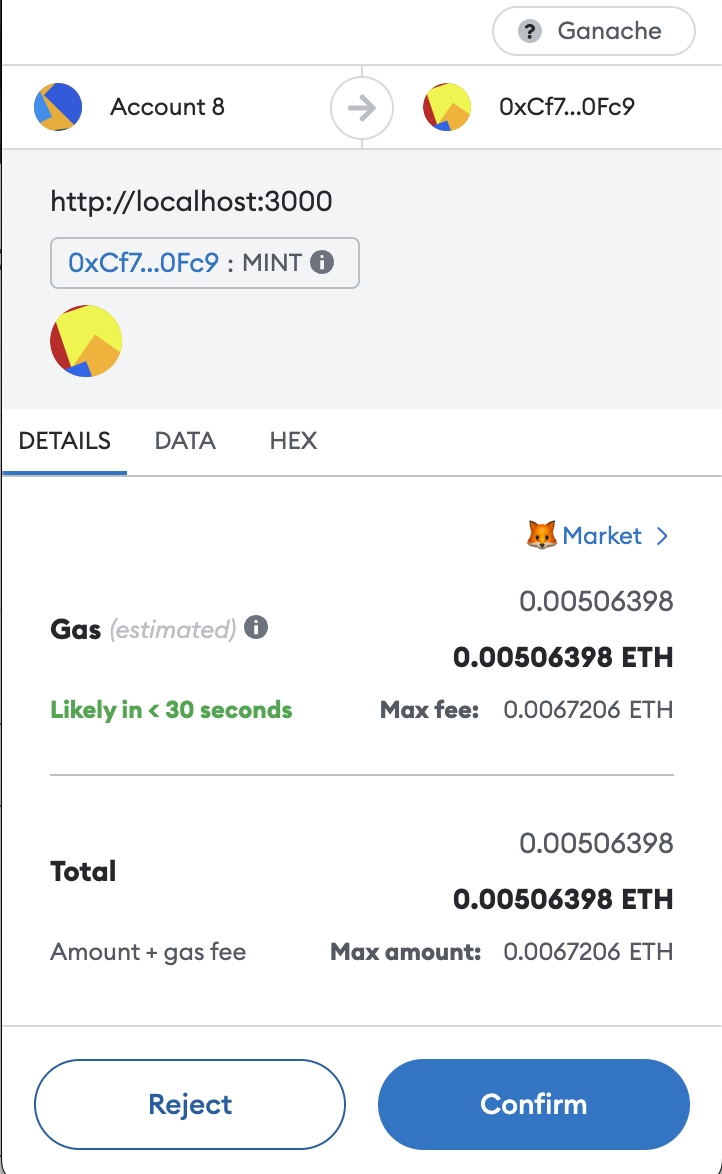
\includegraphics[scale=0.4]{gambar/img-test-buy-mint-1.png}
        \caption{Konfirmasi \emph{minting} token}
        \label{fig:TestBuyKonfirmasiMintingToken}
      \end{figure}
    Pada gambar terlihat bahwa estimasi \emph{gas} adalah \textbf{0,00506398} \emph{ETH}
    \begin{figure} [H] \centering
        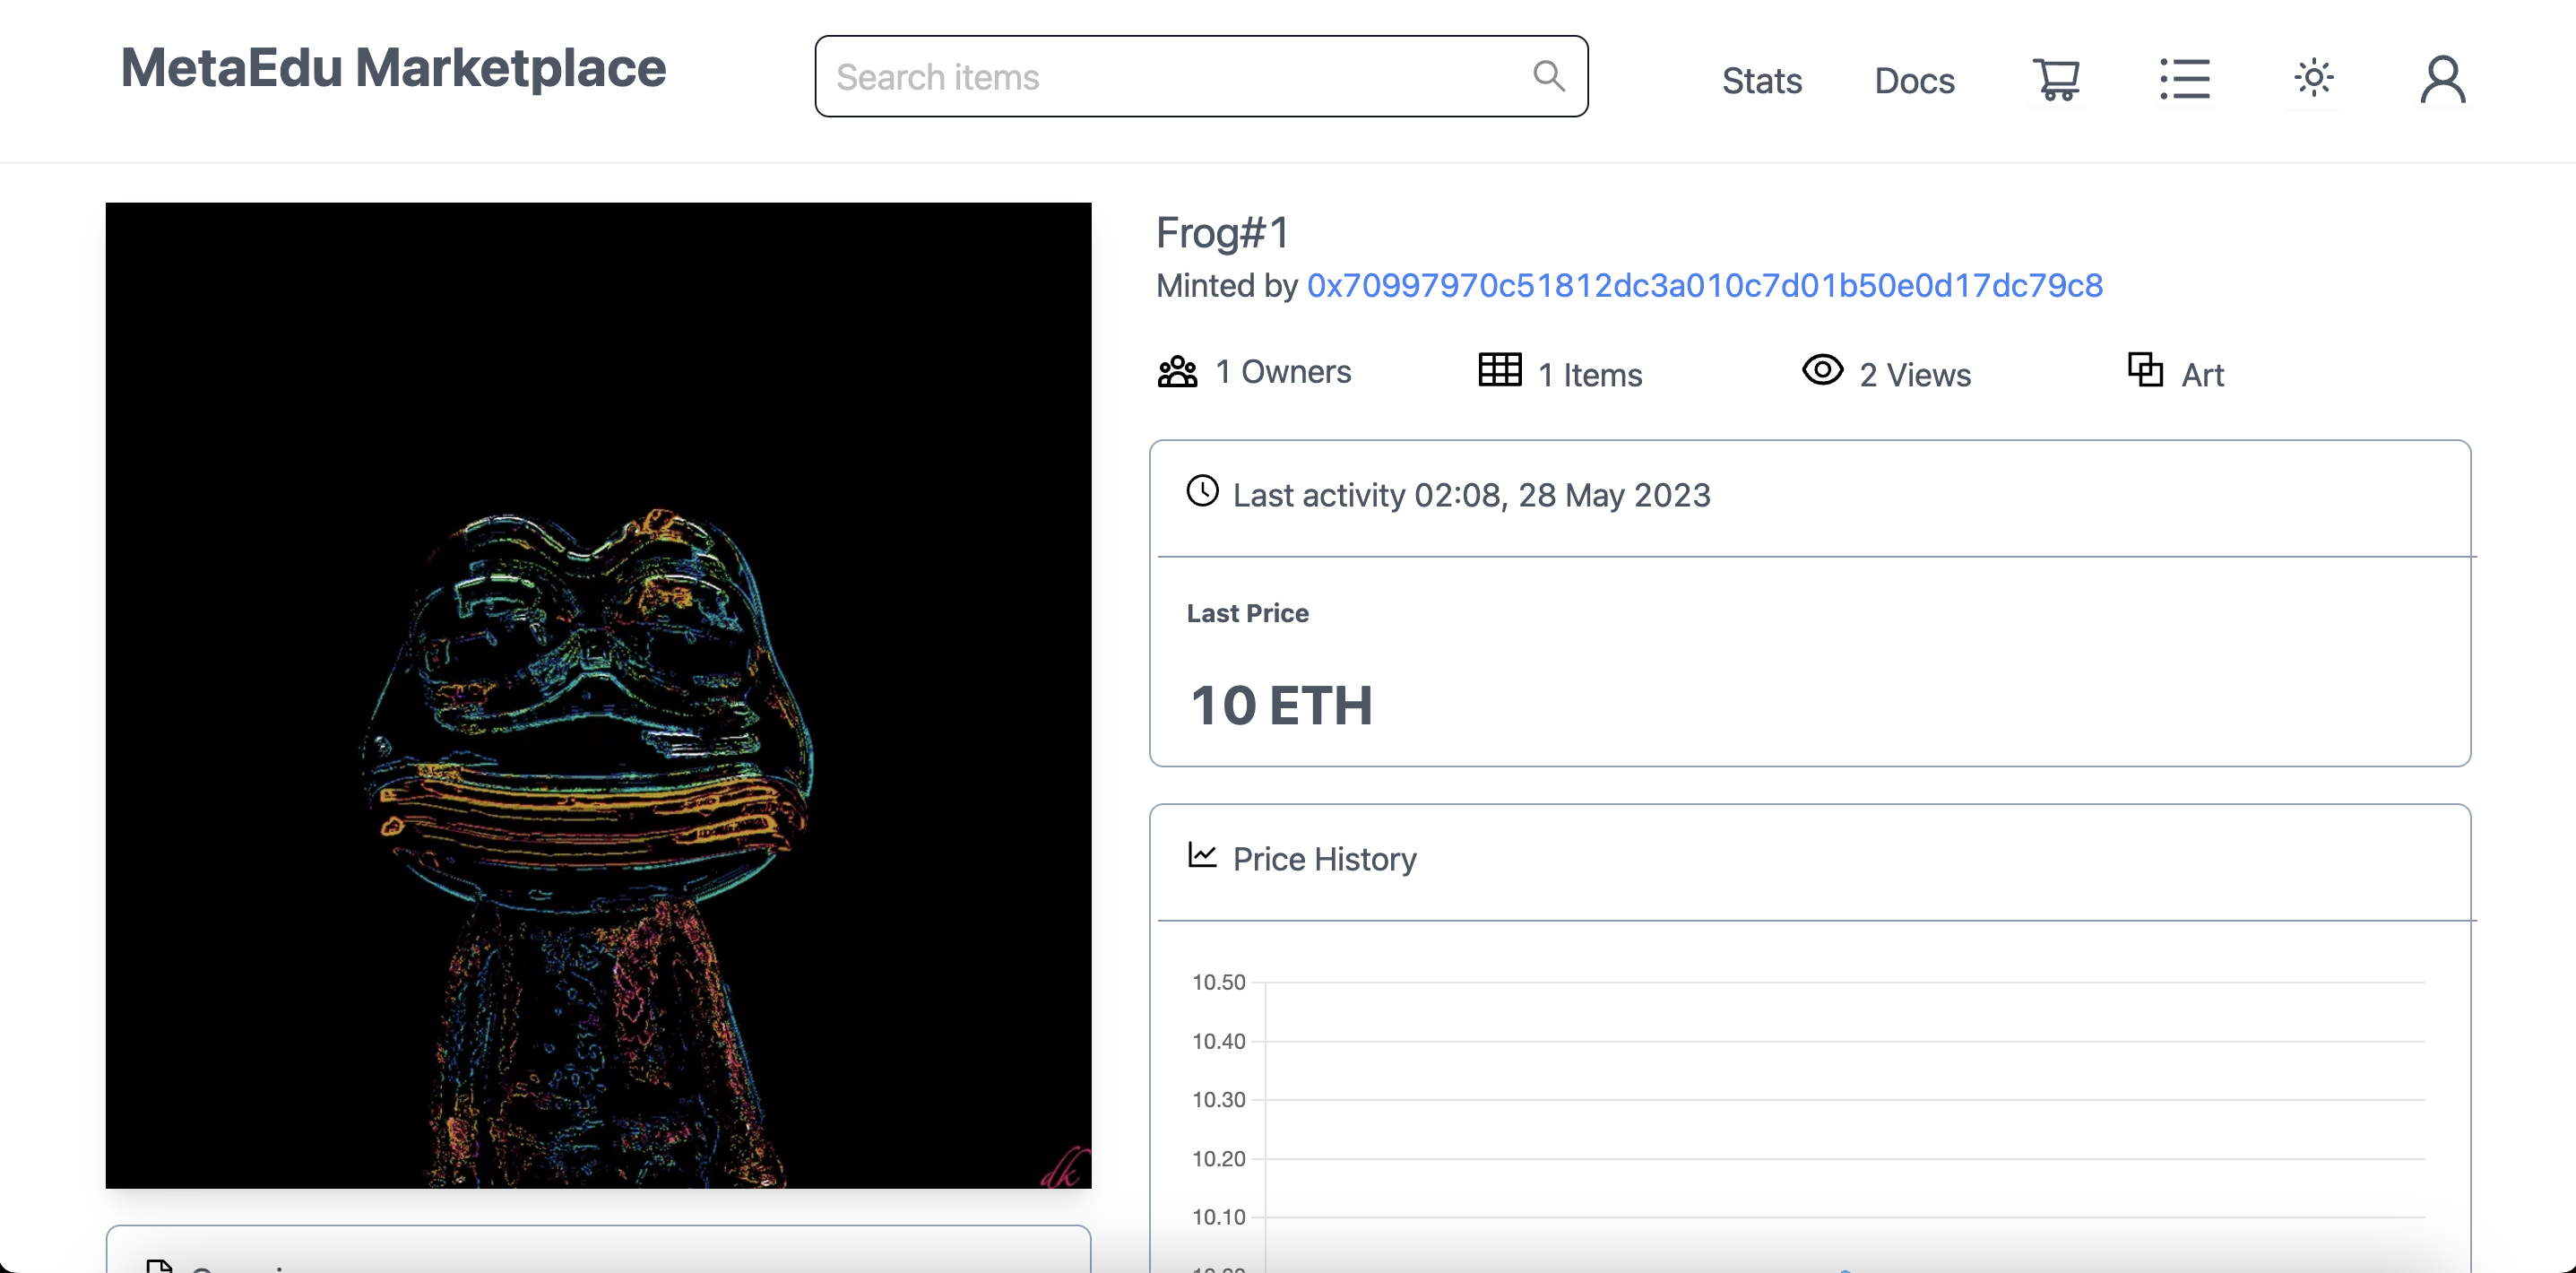
\includegraphics[scale=0.3]{gambar/img-test-buy-mint-2.png}
        \caption{Hasil minting token-1}
        \label{fig:TestBuyHasilMinting}
      \end{figure}
      \begin{figure} [H] \centering
        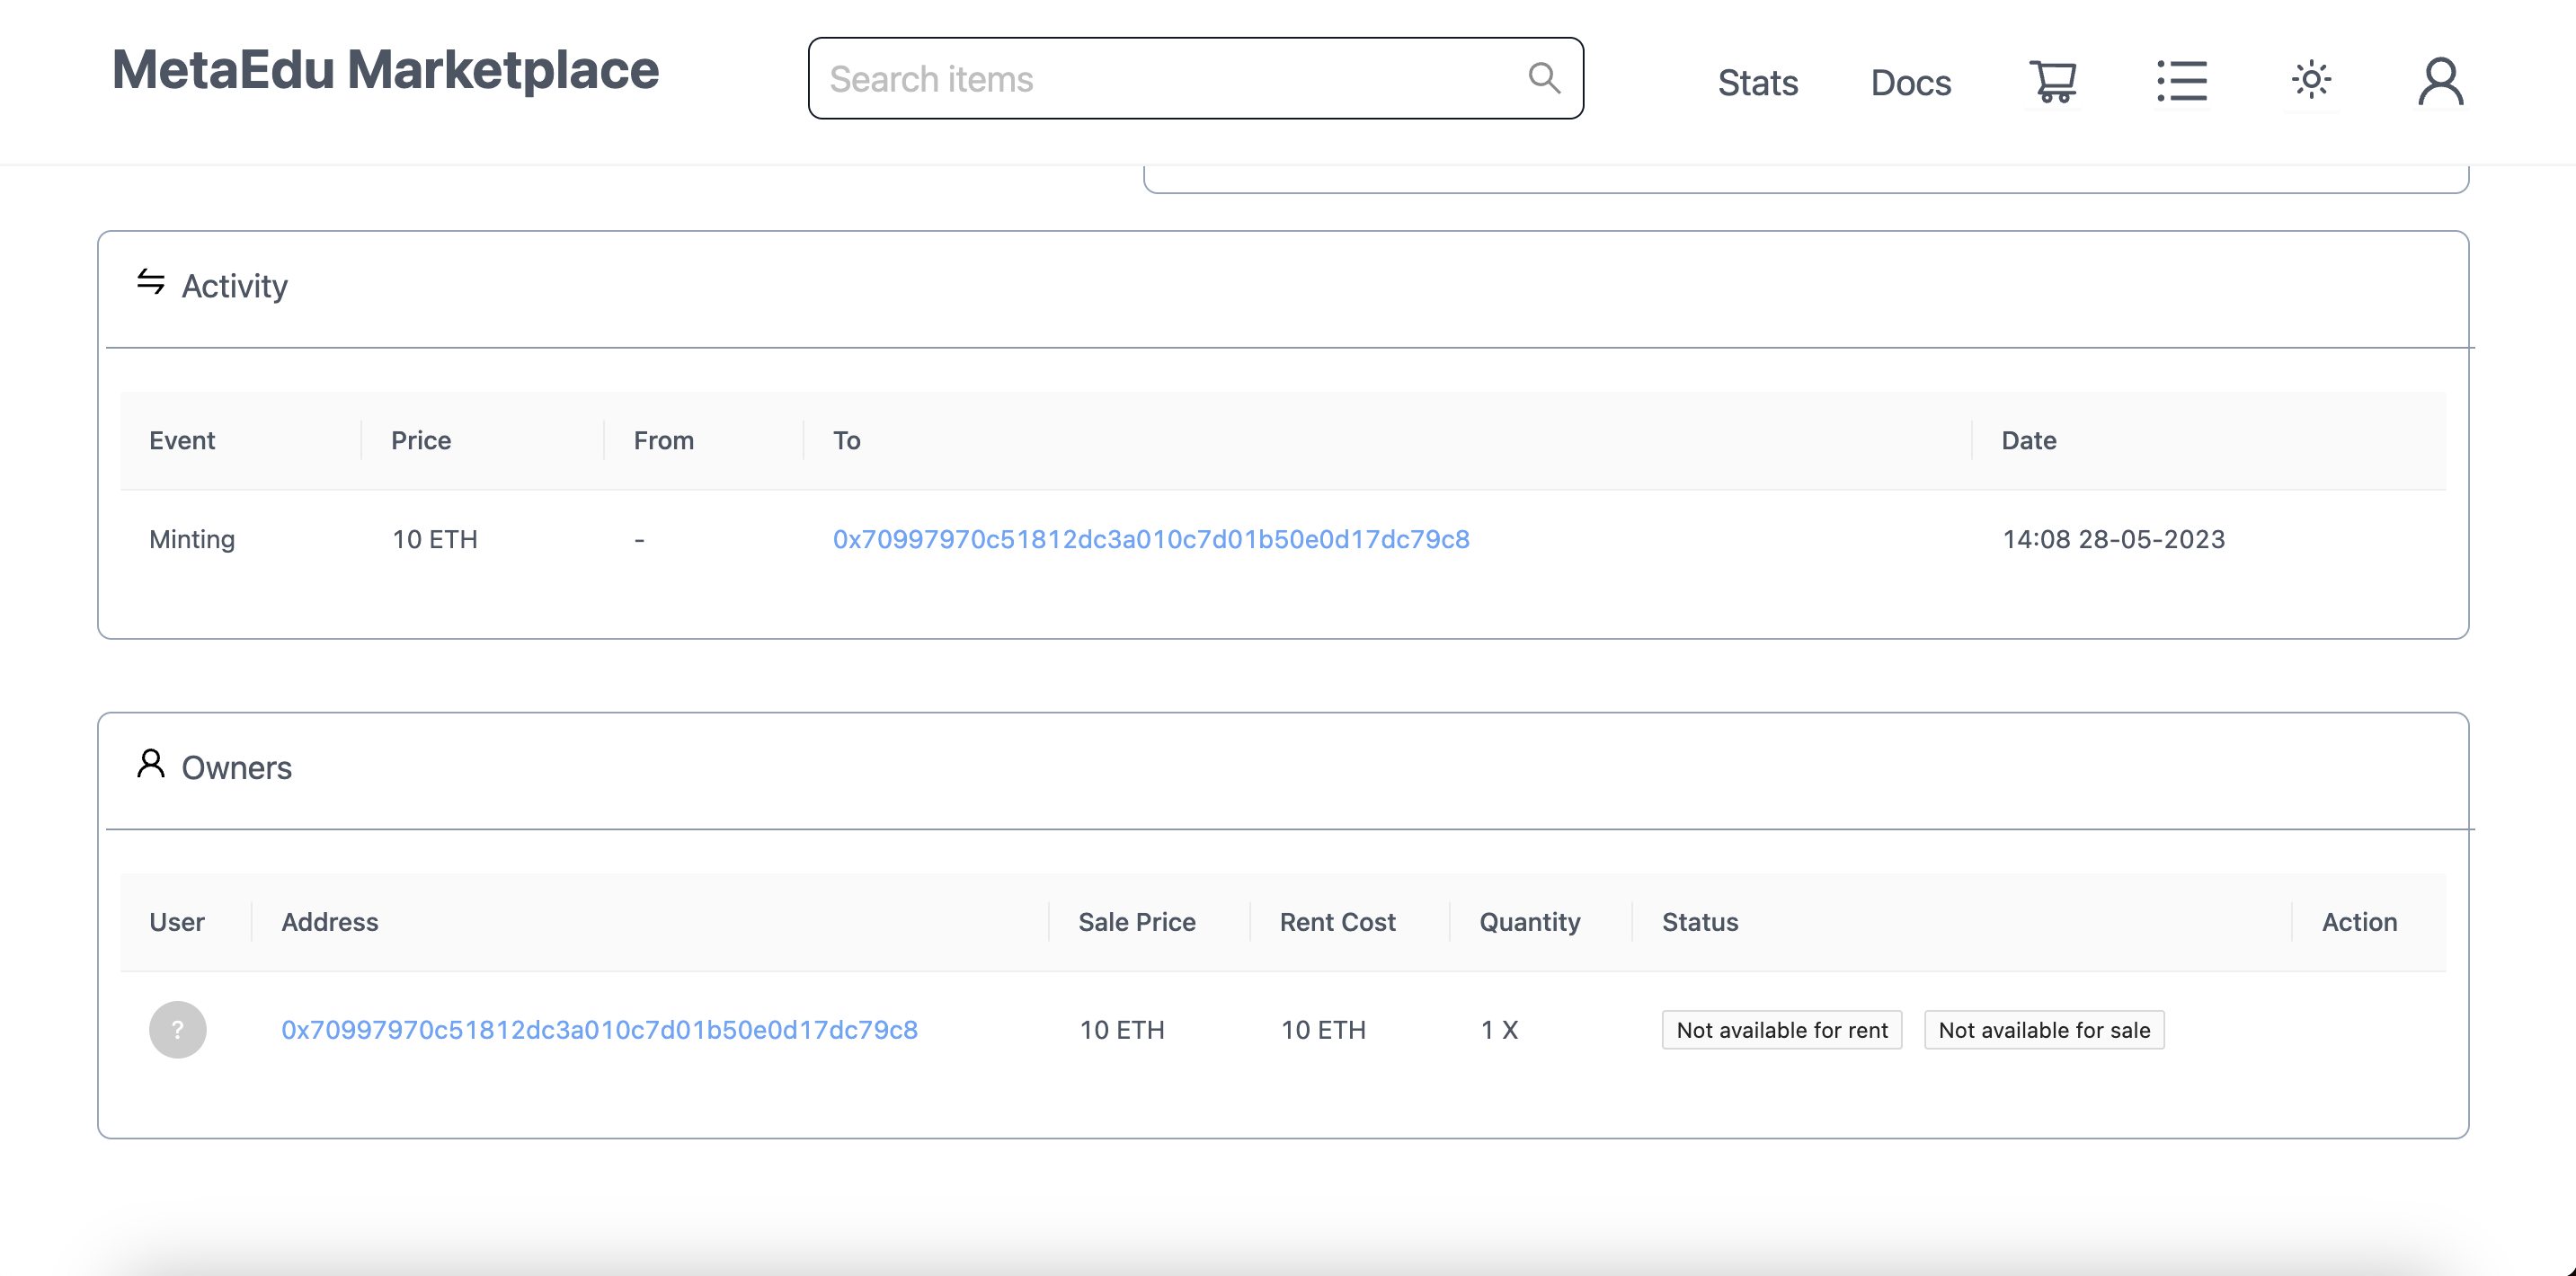
\includegraphics[scale=0.3]{gambar/img-test-buy-mint-3.png}
        \caption{Hasil minting token-2}
        \label{fig:TestBuyHasilMinting}
      \end{figure}
      \begin{figure} [H] \centering
        \includegraphics[scale=0.4]{gambar/img-test-buy-mint-4.png}
        \caption{Hasil minting token pada \emph{Ethernal}}
        \label{fig:TestBuyHasilMinting}
      \end{figure}
    Pada gambar dapat diketahui bahwa \emph{gas} yang diperlukan/\emph{gas used} adalah \textbf{220,513} dan \emph{gas price} adalah \textbf{2,006169455} \emph{gwei} maka \emph{gas fee} yang dibayarkan adalah \textbf{0,000442386445030415} \emph{ETH}
    \item Akun A memperbarui status token yang telah di-\emph{minting} supaya dapat dijual.
    \begin{figure} [H] \centering
        \includegraphics[scale=0.3]{gambar/img-test-buy-put-item-for-sale-1.png}
        \caption{Konfirmasi pembaruan status penjualan token}
        \label{fig:TestBuyKonfirmasiPembaruanPenjual}
      \end{figure}
      Pada gambar dapat diketahu bahwa estimasi \emph{gas fee} adalah \textbf{0,0035833 \emph{ETH}}.
      \begin{figure} [H] \centering
        \includegraphics[scale=0.3]{gambar/img-test-buy-put-item-for-sale-2.png}
        \caption{Hasil pembaruan status penjualan \emph{token} pada \emph{web}}
        \label{fig:TestBuyPutItemForSale}
      \end{figure}
      \begin{figure} [H] \centering
        \includegraphics[scale=0.3]{gambar/img-test-buy-put-item-for-sale-4.png}
        \caption{Hasil pembaruan status penjualan \emph{token} pada \emph{Ethernal}}
        \label{fig:TestBuyPutItemForSaleEthernal}
      \end{figure}
      Pada gambar dapat diketahui bahwa \emph{gas} yang diperlukan/\emph{gas used} adalah \textbf{147,703} dan \emph{gas price} adalah \textbf{1,943828415 \emph{gwei}} maka \emph{gas fee} yang dibayarkan adalah \textbf{0,000287109288380745 \emph{ETH}}.
    \item Akun B membeli \emph{token} yang dimiliki oleh akun A
    \begin{figure} [H] \centering
        \includegraphics[scale=0.4]{gambar/img-test-buy-buy-1.png}
        \caption{Konfirmasi pembelian token}
        \label{fig:TestBuyKonfirmasiPembelianToken}
      \end{figure}
    Pada gambar dapat diketahui bahwa estimasi \emph{gas} adalah \textbf{0,00299872 \emph{ETH}} dan harga pembelian adalah \textbf{10 ETH} sesuai dengan harga jual \emph{token}
    \begin{figure} [H] \centering
        \includegraphics[scale=0.3]{gambar/img-test-buy-buy-2.png}
        \caption{Hasil pembelian token}
        \label{fig:TestBuyHasilPembelian}
      \end{figure}
      Setelah dilakukan pembelian maka \emph{address} \emph{owner} akan menjadi \emph{address} dari akun B dan data pembelian akan tercatat pada tabel \emph{activity}.
      \begin{figure} [H] \centering
        \includegraphics[scale=0.4]{gambar/img-test-buy-buy-5.png}
        \caption{Hasil pembelian token pada \emph{Ethernal}}
        \label{fig:TestBuyHasilPembelian2}
      \end{figure}
      Pada gambar dapat diketahui bahwa \emph{gas} yang diperlukan/\emph{gas used} adalah \textbf{110,635} dan \emph{gas price} adalah \textbf{1,888896154 \emph{gwei}} maka \emph{gas fee} yang dibayarkan adalah \textbf{0.00020897802599779 \emph{ETH}}.
    \begin{figure} [H] \centering
        \includegraphics[scale=0.4]{gambar/img-test-buy-buy-3.png}
        \caption{Saldo akun B setelah melakukan pembelian}
        \label{fig:TestBuyHasilPembelian3}
      \end{figure}
    Saldo dari \emph{wallet} akun B berkurang sebesar \textbf{10 \emph{ETH}} ditambah dengan \emph{gas fee} yang diperlukan pada transaksi sebelumnya menjadi 9989.9998 \emph{ETH}.
    \begin{figure} [H] \centering
        \includegraphics[scale=0.4]{gambar/img-test-buy-buy-4.png}
        \caption{Saldo akun A bertambah setelah token yang dimiliki dibeli}
        \label{fig:TestBuyHasilPembelian4}
      \end{figure}
    Saldo dari \emph{wallet} akun A bertambah sebesar \textbf{10 \emph{ETH}} ditambah dengan \emph{gas fee} yang diperlukan pada transaksi sebelumnya menjadi 9989.9998 \emph{ETH}. 
\end{itemize}

Setelah dilakukan pengujian pembelian maka dapat diketahui bahwa alur dari aplikasi telah berjalan sesuai dengan harapan pengujian yang telah disebutkan di awal dimana salah satunya adalah penjual memperoleh \emph{ETH} sesuai dengan harga token dan jumlah yang dijual yaitu \emph{\textbf{10 ETH}} dan sebaliknya pembeli mendapatkan potongan sebesar \emph{\textbf{10 ETH}}. Selain itu juga diperoleh data mengenai \emph{gas fee} sesuai dengan tabel berikut

\begin{longtable}{|c|c|c|c|}
    \caption{\emph{Gas fee} yang diperoleh selama pengujian \emph{flow} pembelian}
    \label{tb:EnergiKecepatan}                                   \\
    \hline
    \rowcolor[HTML]{C0C0C0}
    \textbf{\emph{Function}}  & \textbf{\emph{Gas used}} & \textbf{\emph{Gas price}}  & \textbf{\emph{Gas fee} yang dibayarkan (\emph{ETH})} \\
    \hline
    \emph{mint}           & 220,513 & 2,006169455  & 0,000442386445030415    \\
    \emph{putItemForSale} & 147,703 & 1,943828415  & 0,000287109288380745    \\
    \emph{buy}            & 110,635 & 1.888896154  & 0.00020897802599779      \\
    \hline
  \end{longtable}

\subsection{\emph{Flow} Penyewaan}

Ekspektasi dari pengujian \emph{flow} penyewaan antara lain adalah sebagai berikut:
\begin{itemize}
    \item Pemilik \emph{token} dapat menyewakan \emph{token} yang dimiliki.
    \item Pengguna lain dapat menyewa \emph{token}.
    \item Saldo \emph{wallet} pemilik bertambah sesuai dengan harga dan lama sewa.
    \item Saldo \emph{wallet} penyewa berkurang sesuai dengan harga dan lama sewa.
    \item Seluruh data terkait dengan kepemilikan dan penyewaan dari \emph{token} di halaman web sesuai dengan alur pengujian  
\end{itemize}

Berikut merupakan data mengenai \emph{wallet} yang digunakan dalam pengujian:

\begin{longtable}{|c|c|c|}
    \caption{Kondisi awal}
    \label{tb:KondisiAwalPengujianSewa}                                   \\
    \hline
    \rowcolor[HTML]{C0C0C0}
    \textbf{\emph{Akun}} & \textbf{\emph{Address}} & \textbf{Saldo (\emph{ETH})}\\
    \hline
    A & 0xcd3B766CCDd6AE721141F452C550Ca635964ce71            & 10000               \\
    B & 0x2546BcD3c84621e976D8185a91A922aE77ECEc30            & 10000               \\
    \hline
  \end{longtable}

Berikut merupakan langkah-langkah pengujian yang akan dilakukan:
  \begin{itemize}
      \item Akun A melakukan \emph{minting token} dengan suplai 1 token dan harga 10 ETH.
      \begin{figure} [H] \centering
          \includegraphics[scale=0.4]{gambar/img-test-rent-mint-1.png}
          \caption{Konfirmasi \emph{minting} token}
          \label{fig:TestRentKonfirmasiMintingToken}
        \end{figure}
      Pada gambar terlihat bahwa estimasi \emph{gas} adalah \textbf{0,00541053} \emph{ETH}
      \begin{figure} [H] \centering
          \includegraphics[scale=0.3]{gambar/img-test-rent-mint-2.png}
          \caption{Hasil minting token-1}
          \label{fig:TestRentHasilMinting}
        \end{figure}
        \begin{figure} [H] \centering
          \includegraphics[scale=0.3]{gambar/img-test-rent-mint-3.png}
          \caption{Hasil minting token-2}
          \label{fig:TestRentHasilMinting2}
        \end{figure}
        \begin{figure} [H] \centering
          \includegraphics[scale=0.4]{gambar/img-test-rent-mint-4.png}
          \caption{Hasil minting token pada \emph{Ethernal}}
          \label{fig:TestRentHasilMinting3}
        \end{figure}
      Pada gambar dapat diketahui bahwa \emph{gas} yang diperlukan/\emph{gas used} adalah \textbf{220,513} dan \emph{gas price} adalah \textbf{2,006169455} \emph{gwei} maka \emph{gas fee} yang dibayarkan adalah \textbf{0,000442386445030415} \emph{ETH}
      \item Akun A memperbarui status token yang telah di-\emph{minting} supaya dapat disewakan.
      \begin{figure} [H] \centering
          \includegraphics[scale=0.3]{gambar/img-test-rent-put-item-for-rent-1.png}
          \caption{Konfirmasi pembaruan status penyewaan token}
          \label{fig:TestRentKonfirmasiPembaruanPenyewa}
        \end{figure}
        Pada gambar dapat diketahu bahwa estimasi \emph{gas fee} adalah \textbf{0,00508287 \emph{ETH}}.
        \begin{figure} [H] \centering
          \includegraphics[scale=0.3]{gambar/img-test-rent-put-item-for-rent-2.png}
          \caption{Hasil pembaruan status penyewaan \emph{token}}
          \label{fig:TestRentPutItemForRent}
        \end{figure}
        \begin{figure} [H] \centering
            \includegraphics[scale=0.3]{gambar/img-test-rent-put-item-for-rent-3.png}
            \caption{Hasil pembaruan status penyewaan \emph{token} pada \emph{Ethernal}}
            \label{fig:TestRentPutItemForRent2}
          \end{figure}
        Pada gambar dapat diketahui bahwa \emph{gas} yang diperlukan/\emph{gas used} adalah \textbf{170,805} dan \emph{gas price} adalah \textbf{1,618386387 \emph{gwei}} maka \emph{gas fee} yang dibayarkan adalah \textbf{0,000276428486831535 \emph{ETH}}.
      \item Akun A memperbarui harga sewa \emph{token} menjadi \textbf{1 \emph{ETH}} per hari
      \begin{figure} [H] \centering
        \includegraphics[scale=0.3]{gambar/img-test-rent-put-item-for-rent-2-1.png}
        \caption{Konfirmasi pembaruan harga sewa token}
        \label{fig:TestRentKonfirmasiPembaruanPenyewa2-1}
      \end{figure}
      Pada gambar dapat diketahu bahwa estimasi \emph{gas fee} adalah \textbf{0,00199656 \emph{ETH}}.
      \begin{figure} [H] \centering
        \includegraphics[scale=0.3]{gambar/img-test-rent-put-item-for-rent-2-2.png}
        \caption{Hasil pembaruan harga penyewaan \emph{token}}
        \label{fig:TestRentPutItemForRent2-2}
      \end{figure}
      \begin{figure} [H] \centering
          \includegraphics[scale=0.3]{gambar/img-test-rent-put-item-for-rent-2-3.png}
          \caption{Hasil pembaruan status penyewaan \emph{token} pada \emph{Ethernal}}
          \label{fig:TestRentPutItemForRent2-3}
        \end{figure}
      Pada gambar dapat diketahui bahwa \emph{gas} yang diperlukan/\emph{gas used} adalah \textbf{74,105} dan \emph{gas price} adalah \textbf{1,603756597 \emph{gwei}} maka \emph{gas fee} yang dibayarkan adalah \textbf{0,000118846382620685 \emph{ETH}}.
      \item Akun B menyewa \emph{token} yang dimiliki oleh akun A selama 3 hari
        \begin{figure} [H] \centering
            \includegraphics[scale=0.4]{gambar/img-test-rent-rent-1.png}
            \caption{Input lama penyewaan \emph{token}}
            \label{fig:TestRentInputRentalPeriodToken}
          \end{figure}

          \begin{figure} [H] \centering
        \includegraphics[scale=0.4]{gambar/img-test-rent-rent-2.png}
        \caption{Konfirmasi penyewaan \emph{token}}
        \label{fig:TestRentKonfirmasiPenyewaanToken}
      \end{figure}
        Pada gambar dapat diketahui bahwa estimasi \emph{gas} adalah \textbf{0,00210825 \emph{ETH}} dan biaya penyewaan adalah \textbf{3 ETH} sesuai dengan harga sewa \emph{token} dan lama penyewaan
      \begin{figure} [H] \centering
          \includegraphics[scale=0.3]{gambar/img-test-rent-rent-3.png}
          \caption{Hasil penyewaan token}
          \label{fig:TestRentResultRental}
        \end{figure}
        Setelah dilakukan penyewaan maka data penyewaan akan tecatat pada tabel \emph{activity}.
        \begin{figure} [H] \centering
          \includegraphics[scale=0.4]{gambar/img-test-rent-rent-4.png}
          \caption{Hasil penyewaan token pada \emph{Ethernal}}
          \label{fig:TestRentResultRental2}
        \end{figure}
        Pada gambar dapat diketahui bahwa \emph{gas} yang diperlukan/\emph{gas used} adalah \textbf{77,737} dan \emph{gas price} adalah \textbf{1,590851097 \emph{gwei}} maka \emph{gas fee} yang dibayarkan adalah \textbf{0.000123667991727489 \emph{ETH}}.
      Saldo dari \emph{wallet} akun B berkurang sebesar \textbf{3 \emph{ETH}} ditambah dengan \emph{gas fee} yang diperlukan pada transaksi sebelumnya menjadi 9989.9998 \emph{ETH}.
      \begin{figure} [H] \centering
          \includegraphics[scale=0.4]{gambar/img-test-rent-rent-5.png}
          \caption{Saldo akun B setelah menyewa \emph{token}}
          \label{fig:TestRentResultRental3}
        \end{figure}
      Saldo dari \emph{wallet} akun A bertambah sebesar \textbf{3 \emph{ETH}} dikurangi dengan \emph{gas fee} yang diperlukan pada transaksi sebelumnya menjadi 9989.9998 \emph{ETH}. 
      \begin{figure} [H] \centering
        \includegraphics[scale=0.4]{gambar/img-test-rent-rent-6.png}
        \caption{Saldo akun A bertambah setelah token yang dimiliki disewa}
        \label{fig:TestRentResultRental4}
      \end{figure}
    \end{itemize}
  
  Setelah dilakukan pengujian penyewaan maka dapat disimpulkan bahwa alur dari aplikasi telah berjalan sesuai dengan harapan pengujian yang telah disebutkan di awal. Selain itu juga diperoleh data mengenai \emph{gas fee} sesuai dengan tabel berikut
  
  \begin{longtable}{|c|c|c|c|}
      \caption{\emph{Gas fee} yang diperoleh selama pengujian \emph{flow} penyewaan}
      \label{tb:EnergiKecepatan}                                   \\
      \hline
      \rowcolor[HTML]{C0C0C0}
      \textbf{\emph{Function}} & \textbf{\emph{Gas used}} & \textbf{\emph{Gas price}} & \textbf{\emph{Gas fee} yang dibayarkan (\emph{ETH})} \\
      \hline
      \emph{mint}  & 203,413 & 1,635037125    & 0,000442386445030415    \\
      \emph{putItemForRent (1)}  & 170,805 & 1,6183836    & 0,000276428486831535    \\
      \emph{putItemForRent (2)} & 74,105 & 1,603756    & 0,000118846382620685      \\
      \emph{rent}               & 77,737 & 1,590851097    & 0.000123667991727489      \\
      \hline
    \end{longtable}

\subsection{\emph{Flow} Pembagian Kepemilikan}

Pada pengujian \emph{flow} pembegaian kepemilikan hal-hal yang diharapkan antara lain adalah:
\begin{itemize}
    \item Pemilik \emph{token} dapat membagi kepemilikan \emph{token} yang dimiliki dengan pengguna lain.
    \item \emph{Token} yang dibagi kepemilikannya akan membuat token asalnya menjadi dimiliki oleh pemilik kontrak dan melakukan \emph{minting} \emph{fraction} \emph{token}  dengan suplai yang merepresentasikan jumlah kepemilikan atas token asal. 
    \item \emph{Token} asal dapat disewakan dan keuntungan dari hasil sewa akan dibagian ke pengguna pemilik \emph{fraction} \emph{token}.
    \item Saldo \emph{wallet} pemilik \emph{fraction token} bertambah sesuai dengan harga dan jumlah kepemilikannya atas \emph{fraction token} dibanding suplai yang beredar.
    \item Saldo \emph{wallet} penyewa berkurang sesuai dengan harga dan lama sewa.
    \item Seluruh data terkait dengan kepemilikan, penjualan, dan penyewaan dari \emph{token} di halaman web sesuai dengan alur pengujian  
\end{itemize}

Berikut merupakan data mengenai \emph{wallet} yang digunakan dalam pengujian:

% Contoh pembuatan tabel
\begin{longtable}{|c|c|c|}
    \caption{Kondisi awal}
    \label{tb:EnergiKecepatan}                                   \\
    \hline
    \rowcolor[HTML]{C0C0C0}
    \textbf{\emph{Akun}} & \textbf{\emph{Address}} & \textbf{Saldo (\emph{ETH})}\\
    \hline
    A & 0xbDA5747bFD65F08deb54cb465eB87D40e51B197E            & 10000               \\
    B & 0x976EA74026E726554dB657fA54763abd0C3a0aa9            & 10000               \\
    C & 0x9965507D1a55bcC2695C58ba16FB37d819B0A4dc            & 10000               \\
    \hline
  \end{longtable}


  Berikut merupakan langkah-langkah pengujian yang akan dilakukan:
  \begin{itemize}
      \item Akun A melakukan \emph{minting token} dengan suplai 1 token dan harga 10 ETH.
      \begin{figure} [H] \centering
          \includegraphics[scale=0.4]{gambar/img-test-share-mint-1.png}
          \caption{Konfirmasi \emph{minting} token}
          \label{fig:TestShareKonfirmasiMintingToken}
        \end{figure}
      Pada gambar terlihat bahwa estimasi \emph{gas} adalah \textbf{0,00498276} \emph{ETH}
      \begin{figure} [H] \centering
          \includegraphics[scale=0.3]{gambar/img-test-share-mint-2.png}
          \caption{Hasil minting token-1}
          \label{fig:TestShareHasilMinting}
        \end{figure}
        \begin{figure} [H] \centering
          \includegraphics[scale=0.3]{gambar/img-test-share-mint-3.png}
          \caption{Hasil minting token-2}
          \label{fig:TestShareHasilMinting2}
        \end{figure}
        \begin{figure} [H] \centering
          \includegraphics[scale=0.4]{gambar/img-test-share-mint-4.png}
          \caption{Hasil minting token pada \emph{Ethernal}}
          \label{fig:TestShareHasilMinting3}
        \end{figure}
      Pada gambar dapat diketahui bahwa \emph{gas} yang diperlukan/\emph{gas used} adalah \textbf{220,413} dan \emph{gas price} adalah \textbf{1,57955364} \emph{gwei} maka \emph{gas fee} yang dibayarkan adalah \textbf{0,000321301729113932} \emph{ETH}
      \item Akun A memperbarui status token yang telah di-\emph{minting} supaya dapat disewakan.
      \begin{figure} [H] \centering
          \includegraphics[scale=0.3]{gambar/img-test-share-put-item-for-rent-1.png}
          \caption{Konfirmasi pembaruan status penyewaan token}
          \label{fig:TestShareKonfirmasiPembaruanPenyewa}
        \end{figure}
        Pada gambar dapat diketahu bahwa estimasi \emph{gas fee} adalah \textbf{0,00425969 \emph{ETH}}.
        \begin{figure} [H] \centering
          \includegraphics[scale=0.3]{gambar/img-test-share-put-item-for-rent-2.png}
          \caption{Hasil pembaruan status penyewaan \emph{token}}
          \label{fig:TestSharePutItemForRent}
        \end{figure}
        \begin{figure} [H] \centering
            \includegraphics[scale=0.3]{gambar/img-test-share-put-item-for-rent-3.png}
            \caption{Hasil pembaruan status penyewaan \emph{token} pada \emph{Ethernal}}
            \label{fig:TestSharePutItemForRent2}
          \end{figure}
        Pada gambar dapat diketahui bahwa \emph{gas} yang diperlukan/\emph{gas used} adalah \textbf{170,805} dan \emph{gas price} adalah \textbf{1,569744221 \emph{gwei}} maka \emph{gas fee} yang dibayarkan adalah \textbf{0,000268120161667905 \emph{ETH}}.
      \item Akun A memperbarui harga sewa \emph{token} menjadi \textbf{1 \emph{ETH}} per hari
      \begin{figure} [H] \centering
        \includegraphics[scale=0.3]{gambar/img-test-share-put-item-for-rent-2-1.png}
        \caption{Konfirmasi pembaruan harga sewa token}
        % Label referensi dari gambar yang diinputkan
        \label{fig:TestShareKonfirmasiPembaruanPenyewa2-1}
      \end{figure}
      Pada gambar dapat diketahu bahwa estimasi \emph{gas fee} adalah \textbf{0,00166636 \emph{ETH}}.
      \begin{figure} [H] \centering
        % Nama dari file gambar yang diinputkan
        \includegraphics[scale=0.3]{gambar/img-test-share-put-item-for-rent-2-2.png}
        % Keterangan gambar yang diinputkan
        \caption{Hasil pembaruan harga penyewaan \emph{token}}
        % Label referensi dari gambar yang diinputkan
        \label{fig:TestSharePutItemForRent2-2}
      \end{figure}
      \begin{figure} [H] \centering
          \includegraphics[scale=0.3]{gambar/img-test-share-put-item-for-rent-2-3.png}
          \caption{Hasil pembaruan status penyewaan \emph{token} pada \emph{Ethernal}}
          \label{fig:TestSharePutItemForRent2-3}
        \end{figure}
        Pada gambar dapat diketahui bahwa \emph{gas} yang diperlukan/\emph{gas used} adalah \textbf{74,105} dan \emph{gas price} adalah \textbf{1,561125466 \emph{gwei}} maka \emph{gas fee} yang dibayarkan adalah \textbf{0,00011568720265793 \emph{ETH}}.
      \item Akun A melakukan \emph{fractionalization} terhadap token yang dimiliki dengan jumlah \emph{token} \emph{fraction} beredar sebanyak 10 dan harga awal 1 \emph{ETH}
        \begin{figure} [H] \centering
            \includegraphics[scale=0.4]{gambar/img-test-share-fraction-1.png}
            \caption{Input suplai dan harga awal \emph{fraction} \emph{token}}
            \label{fig:TestShareInputSupplyFractionToken}
        \end{figure}
        \begin{figure} [H] \centering
            \includegraphics[scale=0.4]{gambar/img-test-share-rent-2.png}
            \caption{Konfirmasi proses \emph{fractionalization} \emph{token}}
            \label{fig:TestShareFractionalizationToken}
        \end{figure}
        \begin{figure} [H] \centering
            \includegraphics[scale=0.3]{gambar/img-test-share-fraction-3.png}
            \caption{Hasil \emph{fractionalization} \emph{token} pada \emph{token} asal-1}
            \label{fig:TestShareResultFractionalizationTokenOnParent1}
        \end{figure}
        \begin{figure} [H] \centering
            \includegraphics[scale=0.3]{gambar/img-test-share-fraction-4.png}
            \caption{Hasil \emph{fractionalization} \emph{token} pada \emph{token} asal-2}
            \label{fig:TestShareResultFractionalizationTokenOnParent2}
        \end{figure}
        Setelah \emph{fractionalization} dilakukan maka terdapat keterangan bahwa \emph{token} tersebut merupakan \emph{parent} dan terdapat \emph{link} yang menghubungkan dengan \emph{token} \emph{fraction}-nya. Selain itu \emph{token} tersebut menjadi milik dari pemilik kontrak.
        \begin{figure} [H] \centering
          \includegraphics[scale=0.3]{gambar/img-test-share-fraction-5.png}
          \caption{Hasil \emph{fractionalization} \emph{token} pada \emph{token} \emph{fraction}}
          \label{fig:TestShareResultFractionalizationTokenOnFraction1}
        \end{figure}
        \begin{figure} [H] \centering
          \includegraphics[scale=0.3]{gambar/img-test-share-fraction-6.png}
          \caption{Hasil \emph{fractionalization} \emph{token} pada \emph{token} \emph{fraction}}
          \label{fig:TestShareResultFractionalizationTokenOnFraction2}
        \end{figure}
        \emph{Fraction} \emph{token} sepenuhnya dimiliki oleh pemilik awal \emph{token} \emph{parent}
        \begin{figure} [H] \centering
          \includegraphics[scale=0.3]{gambar/img-test-share-fraction-7.png}
          \caption{Hasil \emph{fractionalization} \emph{token} pada \emph{Ethernal}}
          \label{fig:TestShareResultFractionalizationTokenOnEthernal}
        \end{figure}
        Pada gambar dapat diketahui bahwa \emph{gas} yang diperlukan/\emph{gas used} adalah \textbf{413,510} dan \emph{gas price} adalah \textbf{1,553522531 \emph{gwei}} maka \emph{gas fee} yang dibayarkan adalah \textbf{0.00064239710179381 \emph{ETH}}.

      \item Akun B membeli sejumlah 5 \emph{token} dari 10 suplai \emph{token} \emph{fraction} yang beredar
        \begin{figure} [H] \centering
            \includegraphics[scale=0.4]{gambar/img-test-share-buy-1.png}
            \caption{Input jumlah \emph{token}}
            \label{fig:TestShareInputRentalPeriodToken}
        \end{figure}
        \begin{figure} [H] \centering
            \includegraphics[scale=0.4]{gambar/img-test-share-buy-2.png}
            \caption{Konfirmasi pembelian \emph{token}}
            \label{fig:TestShareConfirmationBuyToken}
        \end{figure}
        Pada gambar dapat diketahui bahwa estimasi \emph{gas} adalah \textbf{0,00282063 \emph{ETH}} dan biaya penyewaan adalah \textbf{5 ETH} sesuai dengan harga \emph{token} dan jumlah yang dibeli
        \begin{figure} [H] \centering
          \includegraphics[scale=0.3]{gambar/img-test-share-buy-3.png}
          \caption{Hasil pembelian token}
          \label{fig:TestShareResultBuy}
        \end{figure}
        Setelah dilakukan pembelian maka data pembelian akan tecatat pada tabel \emph{activity}.
        \begin{figure} [H] \centering
          \includegraphics[scale=0.4]{gambar/img-test-share-buy-4.png}
          \caption{Hasil pembelian token pada \emph{Ethernal}}
          \label{fig:TestShareResultBuy2}
        \end{figure}
        Pada gambar dapat diketahui bahwa \emph{gas} yang diperlukan/\emph{gas used} adalah \textbf{115,435} dan \emph{gas price} adalah \textbf{1,541197439 \emph{gwei}} maka \emph{gas fee} yang dibayarkan adalah \textbf{0.000177908126370965 \emph{ETH}}.
        
        Saldo dari \emph{wallet} akun B berkurang sebesar \textbf{5 \emph{ETH}} ditambah dengan \emph{gas fee} yang diperlukan pada transaksi sebelumnya menjadi 9994.9998 \emph{ETH}.
        \begin{figure} [H] \centering
            \includegraphics[scale=0.4]{gambar/img-test-share-buy-5.png}
            \caption{Saldo akun B setelah membeli \emph{token}}
            \label{fig:TestShareResultBuy3}
          \end{figure}
        Saldo dari \emph{wallet} akun A bertambah sebesar \textbf{5 \emph{ETH}} dikurangi dengan \emph{gas fee} yang diperlukan pada transaksi sebelumnya menjadi 10004.9984 \emph{ETH}. 
        \begin{figure} [H] \centering
          \includegraphics[scale=0.4]{gambar/img-test-share-buy-6.png}
          \caption{Saldo akun A bertambah setelah \emph{token} \emph{fraction} yang dimiliki dibeli}
          \label{fig:TestShareResultBuy4}
        \end{figure}

      \item Akun C menyewa \emph{token} \emph{parent} yang telah di-\emph{fractionalization} selama 10 hari
        \begin{figure} [H] \centering
            \includegraphics[scale=0.4]{gambar/img-test-share-rent-1.png}
            \caption{Input lama penyewaan \emph{token}}
            \label{fig:TestShareInputRentalPeriodToken}
        \end{figure}
        \begin{figure} [H] \centering
            \includegraphics[scale=0.4]{gambar/img-test-share-rent-2.png}
            \caption{Konfirmasi penyewaan \emph{token}}
            \label{fig:TestShareKonfirmasiPenyewaanToken}
        \end{figure}
        Pada gambar dapat diketahui bahwa estimasi \emph{gas} adalah \textbf{0,00247651 \emph{ETH}} dan biaya penyewaan adalah \textbf{10 ETH} sesuai dengan harga sewa \emph{token} dan lama penyewaan
        \begin{figure} [H] \centering
          \includegraphics[scale=0.3]{gambar/img-test-share-rent-3.png}
          \caption{Hasil penyewaan token}
          \label{fig:TestShareResultRental}
        \end{figure}
        Setelah dilakukan penyewaan maka data penyewaan akan tecatat pada tabel \emph{activity}.
        \begin{figure} [H] \centering
          \includegraphics[scale=0.4]{gambar/img-test-share-rent-4.png}
          \caption{Hasil penyewaan token pada \emph{Ethernal}}
          \label{fig:TestRentResultRental2}
        \end{figure}
        Pada gambar dapat diketahui bahwa \emph{gas} yang diperlukan/\emph{gas used} adalah \textbf{105,945} dan \emph{gas price} adalah \textbf{1,53608739 \emph{gwei}} maka \emph{gas fee} yang dibayarkan adalah \textbf{0.00016274077853355 \emph{ETH}}.
        
        Saldo dari \emph{wallet} akun C berkurang sebesar \textbf{10 \emph{ETH}} ditambah dengan \emph{gas fee} yang diperlukan pada transaksi sebelumnya menjadi 9989.9998 \emph{ETH}.
        \begin{figure} [H] \centering
          \includegraphics[scale=0.4]{gambar/img-test-share-rent-5.png}
          \caption{Saldo akun C setelah menyewa \emph{token}}
          \label{fig:TestShareResultRental3}
        \end{figure}
        Saldo dari \emph{wallet} akun A bertambah sebesar \textbf{5 \emph{ETH}} dikurangi dengan \emph{gas fee} yang diperlukan pada transaksi sebelumnya menjadi 9989.9998 \emph{ETH}. 
        \begin{figure} [H] \centering
          \includegraphics[scale=0.4]{gambar/img-test-share-rent-6.png}
          \caption{Saldo akun A bertambah setelah token \emph{parent} disewa}
          \label{fig:TestShareResultRental4}
        \end{figure}
        Saldo dari \emph{wallet} akun B bertambah sebesar \textbf{5 \emph{ETH}} dikurangi dengan \emph{gas fee} yang diperlukan pada transaksi sebelumnya menjadi 9999.9998 \emph{ETH}. 
        \begin{figure} [H] \centering
          \includegraphics[scale=0.4]{gambar/img-test-share-rent-7.png}
          \caption{Saldo akun B bertambah setelah token \emph{parent} disewa}
          \label{fig:TestShareResultRental6}
        \end{figure}
    \end{itemize}

  Setelah dilakukan pengujian penyewaan maka dapat disimpulkan bahwa alur dari aplikasi telah berjalan sesuai dengan harapan pengujian yang telah disebutkan di awal. Selain itu juga diperoleh data mengenai \emph{gas fee} sesuai dengan tabel berikut
  
  \begin{longtable}{|c|c|c|c|}
      \caption{\emph{Gas fee} yang diperoleh selama pengujian \emph{flow} penyewaan}
    \label{tb:HasilShareOwnership}                                   \\
    \hline
    \rowcolor[HTML]{C0C0C0}
    \textbf{\emph{Function}} & \textbf{Gas used} & \textbf{Gas price} & \textbf{\emph{Gas fee} yang dibayarkan (\emph{ETH})}\\
    \hline
    \emph{mint}  & 203,413 & 1,579553564 & 0,000321301729113932    \\
    \emph{putItemForRent}  & 170,805 & 1,56797 & 0,000268120161667905    \\
    \emph{shareOwnership} & 413,510 &  1,553522 & 0.00064239710179381    \\
    \emph{buy} & 115,435 & 1,541197    & 0.000177908126370965    \\
    \emph{rent} & 105,945 & 1,53608739   & 0.00016274077853355    \\
    \hline
  \end{longtable}

\section{Pengujian Integrasi}
\label{sec:skenariopengujian}

Pengujian ini bertujuan untuk mengetahui apakah integrasi dapat dilakukan secara sinkron antara data yang ada pada \emph{marketplace} dan \emph{platform} lain. Untuk pengujian ini \emph{platform} yang digunakan pengujian adalah \emph{game} buatan sendiri dengan visualisasi 3D dimana setiap pengguna yang mengakses perlu melakukan autentikasi menggunakan \emph{metamask}. 

Dalam 3 tahap pengujian di bawah ini data akun yang digunakan adalah sebagai berikut:

\begin{longtable}{|c|c|c|}
    \caption{Kondisi awal akun pada pengujian pembelian}
    \label{tb:KondisiAwalPengujianPembelian}                                   \\
    \hline
    \rowcolor[HTML]{C0C0C0}
    \textbf{\emph{Akun}} & \textbf{\emph{Address}} & \textbf{Peran}\\
    \hline
    A & 0x619b9339953b3e7DFc1636eaA87609448aBed939            & Platform               \\
    B & 0x7282188d17388653b2cD5b4d14515614dBd43239            & User 1               \\
    C & 0xDfAC3550d562AF660e4D325309629fe925775453            & User 2               \\
    \hline
  \end{longtable}

\subsection{Pengujian \emph{Minting}}

Langkah pertama dari suatu \emph{platform} dalam melakukan integrasi adalah melakukan proses \emph{minting}. Proses \emph{minting} dilakukan oleh akun A sebagai \emph{address} dari \emph{platform}. Ekspektasi setelah dilakukan proses \emph{minting} adalah di dalam \emph{game} tersebut akun A akan memiliki 3 \emph{NFT} sedangkan akun lainnya belum memiliki \emph{NFT} dikarenakan \emph{NFT} baru pada tahap proses \emph{minting} dan belum diperjual belikan atau disewakan. Berikut merupakan hasil proses \emph{minting} pada \emph{marketplace}.

  \begin{figure} [H] \centering
            \includegraphics[scale=0.2]{gambar/img-test-integration-mint-profile-1.png}
            \caption{Kepemilikan akun A pada \emph{Marketplace}}
            \label{fig:TestIntegrationMintingProfile1}
        \end{figure}

  \begin{figure} [H] \centering
            \includegraphics[scale=0.2]{gambar/img-test-integration-mint-profile-2.png}
            \caption{Kepemilikan akun B pada \emph{Marketplace}}
            \label{fig:TestIntegrationMintingProfile2}
        \end{figure}
        
  \begin{figure} [H] \centering
            \includegraphics[scale=0.2]{gambar/img-test-integration-mint-profile-3.png}
            \caption{Kepemilikan akun C pada \emph{Marketplace}}
            \label{fig:TestIntegrationMintingProfile3}
        \end{figure}

Kemudian berikut merupakan tampilan di \emph{platform game} pada masing-masing akun.

\begin{figure} [H] \centering
            \includegraphics[scale=0.2]{gambar/img-test-integration-mint-game-1.png}
            \caption{Kepemilikan akun A pada \emph{game}}
            \label{fig:TestIntegrationMintingGame1}
        \end{figure}

\begin{figure} [H] \centering
            \includegraphics[scale=0.2]{gambar/img-test-integration-mint-game-2.png}
            \caption{Kepemilikan akun B pada \emph{game}}
            \label{fig:TestIntegrationMintingGame2}
        \end{figure}
        
\begin{figure} [H] \centering
            \includegraphics[scale=0.2]{gambar/img-test-integration-mint-game-3.png}
            \caption{Kepemilikan akun C pada \emph{game}}
            \label{fig:TestIntegrationMintingGame3}
        \end{figure}

Setelah dilakukan proses \emph{minting} dapat diketahui bahwa akun A yang memiliki 3 NFT sedangkan akun lain tidak sama sekali. Hasil yang tersebut sesuai dengan ekspektasi pengujian dimana data yang ditampilkan pada profil \emph{marketplace} sama dengan \emph{platform game}. 

\subsection{Pengujian Pembelian}

Setelah melakukan proses \emph{minting}, supaya \emph{NFT} dapat digunakan \emph{user}, \emph{user} harus melakukan pembelian \emph{NFT} yang dimiliki oleh akun pemilik \emph{platform}. Skenario pengujiannya adalah dengan akun B melakukan pembelian terhadap salah satu \emph{NFT} dari akun A. Ekspektasi setelah dilakukan proses pembelian adalah \emph{user} yang melakukan pembelian akan memiliki \emph{NFT} baik pada \emph{marketplace} maupun di \emph{platform game} tersebut. Berikut merupakan hasil dari pembelian \emph{NFT} pada \emph{Marketplace}.

  \begin{figure} [H] \centering
            \includegraphics[scale=0.2]{gambar/img-test-integration-purchase-metamask-1.png}
            \caption{Konfirmasi pembelian akun B terhadap akun A}
            \label{fig:TestIntegrationPurchaseMetamask1}
        \end{figure}

        
  \begin{figure} [H] \centering
            \includegraphics[scale=0.2]{gambar/img-test-integration-purchase-history-1.png}
            \caption{Aktivitias token setelah dilakukan proses pembelian}
            \label{fig:TestIntegrationPurchaseHistory1}
        \end{figure}


Berikut merupakan hasil proses pembelian pada masing-masing akun dalam \emph{marketplace}.

  \begin{figure} [H] \centering
            \includegraphics[scale=0.2]{gambar/img-test-integration-purchase-profile-1.png}
            \caption{Kepemilikan akun A pada \emph{Marketplace}}
            \label{fig:TestIntegrationPurchaseProfile1}
        \end{figure}

  \begin{figure} [H] \centering
            \includegraphics[scale=0.2]{gambar/img-test-integration-purchase-profile-2.png}
            \caption{Kepemilikan akun B pada \emph{Marketplace}}
            \label{fig:TestIntegrationPurchaseProfile2}
        \end{figure}
        
  \begin{figure} [H] \centering
            \includegraphics[scale=0.2]{gambar/img-test-integration-purchase-profile-3.png}
            \caption{Kepemilikan akun C pada \emph{Marketplace}}
            \label{fig:TestIntegrationPurchaseProfile3}
        \end{figure}

Kemudian berikut merupakan tampilan di \emph{platform game} pada masing-masing akun.

\begin{figure} [H] \centering
            \includegraphics[scale=0.2]{gambar/img-test-integration-purchase-game-1.png}
            \caption{Kepemilikan akun A pada \emph{game}}
            \label{fig:TestIntegrationPurchaseGame1}
        \end{figure}

\begin{figure} [H] \centering
            \includegraphics[scale=0.2]{gambar/img-test-integration-purchase-game-2.png}
            \caption{Kepemilikan akun B pada \emph{game}}
            \label{fig:TestIntegrationPurchaseGame2}
        \end{figure}
        
\begin{figure} [H] \centering
            \includegraphics[scale=0.2]{gambar/img-test-integration-purchase-game-3.png}
            \caption{Kepemilikan akun C pada \emph{game}}
            \label{fig:TestIntegrationPurchaseGame3}
        \end{figure}

Setelah dilakukan pembelian dapat diketahui bahwa akun A yang awalnya memiliki 3 NFT setelah dilakukan proses pembelian menjadi memiliki 2 NFT baik pada \emph{marketplace} maupun dalam \emph{platform game}. Sedangkan akun B yang melakukan pembelian memiliki 1 \emph{NFT} baik pada \emph{marketplace} maupun dalam \emph{platform} game. Sedangkan akun C dikarenakan tidak melakukan aksi apapun masih tidak memiliki \emph{NFT}. Hasil yang tersebut sesuai dengan ekspektasi pengujian dimana data yang ditampilkan pada profil \emph{marketplace} sama dengan \emph{platform game}. 

\subsection{Pengujian Penyewaan}

Kemudian adalah pengujian penyewaan dimana pengguna dapat memiliki akses terbatas terhadap \emph{NFT} tanpa perlu melakukan pembelian. Skenario pengujiannya adalah dengan akun C melakukan penyewaan terhadap salah satu \emph{NFT} dari akun A. Ekspektasi setelah dilakukan proses penyewaan adalah \emph{user} yang melakukan penyewaan akan terdaftar sebagai penyewa \emph{NFT} pada \emph{marketplace} dan memiliki akses pada \emph{platform game} tersebut. Berikut merupakan hasil dari penyewaan \emph{NFT} pada \emph{Marketplace}.

  \begin{figure} [H] \centering
            \includegraphics[scale=0.2]{gambar/img-test-integration-rental-metamask-1.png}
            \caption{Konfirmasi penyewaan akun C terhadap akun A}
            \label{fig:TestIntegrationPurchaseMetamask1}
        \end{figure}

        
  \begin{figure} [H] \centering
            \includegraphics[scale=0.2]{gambar/img-test-integration-rental-history-1.png}
            \caption{Aktivitias token setelah dilakukan proses penyewaan}
            \label{fig:TestIntegrationPurchaseHistory1}
        \end{figure}


Berikut merupakan hasil proses penyewaan pada masing-masing akun dalam \emph{marketplace}.

  \begin{figure} [H] \centering
            \includegraphics[scale=0.2]{gambar/img-test-integration-rental-profile-1.png}
            \caption{Kepemilikan akun A pada \emph{Marketplace}}
            \label{fig:TestIntegrationPurchaseProfile1}
        \end{figure}

  \begin{figure} [H] \centering
            \includegraphics[scale=0.2]{gambar/img-test-integration-rental-profile-2.png}
            \caption{Kepemilikan akun B pada \emph{Marketplace}}
            \label{fig:TestIntegrationPurchaseProfile2}
        \end{figure}
        
  \begin{figure} [H] \centering
            \includegraphics[scale=0.2]{gambar/img-test-integration-rental-profile-3.png}
            \caption{Kepemilikan akun C pada \emph{Marketplace}}
            \label{fig:TestIntegrationPurchaseProfile3}
        \end{figure}

Kemudian berikut merupakan tampilan di \emph{platform game} pada masing-masing akun.

\begin{figure} [H] \centering
            \includegraphics[scale=0.2]{gambar/img-test-integration-rental-game-1.png}
            \caption{Kepemilikan akun A pada \emph{game}}
            \label{fig:TestIntegrationPurchaseGame1}
        \end{figure}

\begin{figure} [H] \centering
            \includegraphics[scale=0.2]{gambar/img-test-integration-rental-game-2.png}
            \caption{Kepemilikan akun B pada \emph{game}}
            \label{fig:TestIntegrationPurchaseGame2}
        \end{figure}
        
\begin{figure} [H] \centering
            \includegraphics[scale=0.2]{gambar/img-test-integration-rental-game-3.png}
            \caption{Kepemilikan akun C pada \emph{game}}
            \label{fig:TestIntegrationPurchaseGame3}
        \end{figure}

Setelah dilakukan penyewaan dapat diketahui bahwa akun A masih tetap memiliki 2 \emph{NFT} pada \emph{marketplace} akan tetapi pada \emph{NFT} yang disewa terdapat keterangan batas masa penyewaan. Sedangkan pada \emph{platform game} hanya memiliki 1 \emph{NFT} dikarenakan \emph{NFT} yang lain sedang disewa. Sedangkan akun B yang tidak melakukan transaksi apapun jumlah kepemilikan masih sama. Sedangkan akun C setelah melakukan penyewaan memiliki 1 \emph{NFT} yang masuk dalam kategori penyewaan pada \emph{marketplace} dan 1 \emph{NFT} yang dapat digunakan dalam \emph{platform game}. Hasil yang tersebut sesuai dengan ekspektasi pengujian dimana data yang ditampilkan pada profil \emph{marketplace} sama dengan \emph{platform game}. 

\section{Evaluasi Pengujian}
\label{sec:analisispengujian}

Dari pengujian yang telah dilakukan terhadap masing-masing alur aplikasi \emph{marketplace} hingga integrasi dengan \emph{platform} lain dapat disimpulkan bahwa \emph{NFT Marketplace} yang dikembangkan telah berjalan sesuai dengan yang direncanakan di awal. Hal ini dibuktikan dimana pada hasil setiap pengujian telah memenuhi seluruh ekspektasi yang telah disebutkan di awal skenario pengujian seperti kesesuaian perubahan data kepemilikan, data penjualan, data penyewaan, hingga perolehan \emph{ETH} oleh pemilik token atas penjual atau penyewaan dan sebaliknya pengeluarkan \emph{ETH} yang sesuai dengan perhitungan di awal. Selain itu \emph{gas used} yang dihasilkan dari setiap eksekusi \emph{custom function smart contract} seperti \emph{buy, rent, putItemForSale, putItemForRent} mayoritas masih di bawah \emph{function mint} yang merupakan \emph{function} bawaan dari \emph{function-function} standar yang dimiliki oleh \emph{ERC-1155} sehingga masih relatif efisien. 

\cleardoublepage

% Bab 5 penutup
\chapter{PENUTUP}
\label{chap:penutup}

\section{Kesimpulan}
\label{sec:kesimpulan}

Berdasarkan pengembangan dan pengujian yang telah dilakukan dari NFT Marketplace NFT untuk Metaverse berbasis Blockchain Ethereum, diperoleh beberapa kesimpulan sebagai berikut:
1. Pengguna NFT Marketplace dapat melakukan pembelian, penyewaan, hingga pembagian kepemilikan pada \emph{NFT} yang dimiliki sehingga meningkatkan kemanfaatan dan keuntungan atas \emph{NFT} yang mereka miliki. 
2.  Hasil pengujian gas menunjukan fungsi-fungsi tambahan yang dikembangkan seperti penyewaan dan pembagian kepemilikan sudah cukup efisien jika dibandingkan fungsi bawaan yang disediakan oleh ERC-1155.
3. Selain itu sistem juga dapat diintegrasikan dengan \emph{platform} lain melalui \emph{API} yang disediakan dengan baik.

\section{Saran}
\label{chap:saran}

\begin{enumerate}[nolistsep]
\item \emph{API} yang dikembangkan saat ini masih tidak terproteksi sehingga apabila penggunaannya terlalu masif maka akan berpotensi menurunkan performa \emph{server}. Hal ini dapat diatas dengan adanya \emph{access key} yang diperlukan sebelum \emph{platform} lain menggunakan \emph{API} yang disediakan
\item Pengembangan \emph{NFT Marketplace} untuk \emph{platform mobile} mengingat mayoritas pengguna internet saat ini mengakses internet melalui \emph{device} \emph{mobile} seperti \emph{smartphone}
\item Integrasi dengan sistem orkestrasi seperti \emph{Kubernetes} untuk menunjang skalibilitas dari aplikasi
\item Pembuatan \emph{automation testing} untuk meminimalisir adanya \emph{bug} apabila terdapat pengembangan lebih lanjut
\end{enumerate}
\cleardoublepage

\chapter*{DAFTAR PUSTAKA}
\addcontentsline{toc}{chapter}{DAFTAR PUSTAKA}
\renewcommand\refname{}
\vspace{2ex}
\renewcommand{\bibname}{}
\begingroup
\def\chapter*#1{}
\printbibliography
\endgroup
\cleardoublepage

% Biografi penulis
\begin{center}
  \Large
  \textbf{BIOGRAFI PENULIS}
\end{center}

\addcontentsline{toc}{chapter}{BIOGRAFI PENULIS}

\vspace{2ex}

\begin{wrapfigure}{L}{0.3\textwidth}
  \centering
  \vspace{-3ex}
  % Ubah file gambar berikut dengan file foto dari mahasiswa
  \includegraphics[width=0.3\textwidth]{gambar/img-writer.jpg}
  \vspace{-4ex}
\end{wrapfigure}

% Ubah kalimat berikut dengan biografi dari mahasiswa
\name{}, lahir pada 28 janurari 2001 di
Pati, Jawa Tengah. Penulis lulus dari SMP Negeri 3 Pati pada tahun 2016 kemudian melanjutkan pendidikan ke SMA Negeri 1 Pati hingga akhirnya lulus pada tahun 2019. Penulis kemudian melanjutkan pendidikan S-1 ke Departemen Teknik Kom-
puter, FTEIC-ITS Surabaya. Saat di kuliah penulis aktif menjadi Assistant Laboratorium
B201. Bagi pembaca yang memiliki kritik, saran atau pertanyaan mengenai penelitian ini dapat menghubungi penulis melalui email

renakaagusta28@gmail.com.

\cleardoublepage

\end{document}
